\documentclass[ebook, 12pt, twoside]{memoir}

%% \makeatletter
%% \renewcommand\@dotsep{10000}
%% \renewcommand{\l@part}{\l@chapter}
%% \renewcommand{\l@section}{\@dottedtocline{1}{1.5em}{2.6em}}
%% \renewcommand{\l@subsection}{\@dottedtocline{2}{4.0em}{3.6em}}
%% \renewcommand{\l@subsubsection}{\@dottedtocline{3}{7.4em}{4.5em}}
%% \makeatother

\noindexintoc

\usepackage{relsize}
\usepackage{afterpage}

\newcommand\blankpage{%
    \null
    \thispagestyle{empty}%
    \addtocounter{page}{-1}%
    \newpage}

\usepackage{enumitem}
\usepackage{array}
\def\Tiny{\fontsize{8pt}{8pt} \selectfont}

\renewcommand*{\cftchapterfont}{\bfseries}

\makeatletter
\def\below{\xdef\@thefnmark{}\@footnotetext}
\makeatother

%\usepackage{amsmath}
%\usepackage{times}
%\usepackage[MnSymbol]{mathspec}
%\setmathsfont(Digits,Latin,Greek)[Numbers={Lining,Proportional}]{Linux Libertine O}
%\setminwhitespace % not sure if this helps
%\setmathrm{Linux Biolinum O}

\usepackage[MnSymbol]{mathspec}
\setmathsfont(Digits,Latin,Greek)[Numbers={Lining,Proportional}]{Linux Libertine O}
\setminwhitespace % not sure if this helps
\setmathrm{Linux Biolinum O}

\usepackage{xunicode}
\defaultfontfeatures{Mapping=tex-text}
%\setmainfont{Linux Libertine O}

\usepackage{metalogo}
\usepackage{caption}
%% \setmainfont[Mapping= tex-text,  
%%      SmallCapsFont={Linux Libertine O},   
%%      SmallCapsFeatures= {Color=6600CC, RawFeature={+smcp,+hlig,+dlig}},   
%%      BoldFont={Linux Biolinum O Bold},   
%%      BoldFeatures={Color = E6005C,SmallCapsFont={Linux Libertine Capitals O Bold},%
%%        SmallCapsFeatures = { Color=F2521B,   RawFeature={+smcp,+hlig,+dlig}} },  
%%      ItalicFont={Linux Libertine O Italic},   
%%      ItalicFeatures={Color = 00CC00, RawFeature={+liga,+hlig,+dlig}, %
%%        SmallCapsFont={Linux Libertine Capitals O Italic}, %
%%        SmallCapsFeatures = {Color=00FFFF,RawFeature={+smcp,+hlig,+dlig}}},   
%%      BoldItalicFont={Linux Biolinum O},   
%%      BoldItalicFeatures={ Color = 3366FF, %
%%       SmallCapsFont={Linux Libertine Capitals O Bold Italic},  %
%%       SmallCapsFeatures = { Color=3366FF,RawFeature={+smcp,+hlig,+dlig}}} ]{Linux Libertine O} 

\setmainfont[Mapping= tex-text,  
     SmallCapsFont={Linux Libertine O},   
     SmallCapsFeatures= {Color=FFFFFF, RawFeature={+smcp,+hlig,+dlig}},   
     BoldFont={Linux Biolinum O Bold},   
%     BoldFeatures={Color = FFFFFF,SmallCapsFont={Linux Libertine Capitals O Bold},%
%       SmallCapsFeatures = { Color=FFFFFF,   RawFeature={+smcp,+hlig,+dlig}} },  
     ItalicFont={Linux Libertine O Italic},   
     ItalicFeatures={Color = FFFFFF,  %
       SmallCapsFont={Linux Libertine Capitals O Italic}, %
       SmallCapsFeatures = {Color=FFFFFF}},   
     BoldItalicFont={Linux Biolinum O},   
     BoldItalicFeatures={ Color = FFFFFF, %
      SmallCapsFont={Linux Libertine Capitals O Bold Italic},  %
      SmallCapsFeatures = { Color=FFFFFF,RawFeature={+smcp,+hlig,+dlig}}} ]{Linux Libertine O} 

\let\sc\scshape

\newcommand{\hookuparrow}{%
    \mathrel{\raisebox{2pt}{\reflectbox{\rotatebox[origin=c]{180}{$\hookrightarrow$}}}}}

\newfontfamily\calligraphicfont{Linux Biolinum Shadow O}
\newcommand\calP{\text{\upshape\calligraphicfont P}}
\newcommand\calU{\text{\upshape\calligraphicfont U}}
\newcommand\calV{\text{\upshape\calligraphicfont V}}
\newcommand\calF{\text{\upshape\calligraphicfont F}}
\newcommand\calB{\text{\upshape\calligraphicfont B}}
\newcommand\calE{\text{\upshape\calligraphicfont E}}
\newcommand\calX{\text{\upshape\calligraphicfont X}}
\newcommand\calJ{\text{\upshape\calligraphicfont J}}

\makeatletter
\newcommand*{\shfttext}[2]{%
  \settowidth{\@tempdima}{#2}%
  \makebox[\@tempdima]{\hspace*{#1}#2}%
}
\makeatother

%\usepackage{xunicode}
%\defaultfontfeatures{Mapping=tex-text}
%\setmainfont{Linux Libertine O}

 %% \setmainfont[Mapping= tex-text,  
 %%     SmallCapsFont={Linux Libertine O},   
 %%     SmallCapsFeatures= {Color=6600CC, RawFeature={+smcp,+hlig,+dlig}},   
 %%     BoldFont={Linux Biolinum O Bold},   
 %%     BoldFeatures={Color = E6005C,SmallCapsFont={Linux Libertine Capitals O Bold},%
 %%       SmallCapsFeatures = { Color=996600,   RawFeature={+smcp,+hlig,+dlig}} },  
 %%     ItalicFont={Linux Libertine O Italic},   
 %%     ItalicFeatures={Color = 00CC00, RawFeature={+liga,+hlig,+dlig}, %
 %%       SmallCapsFont={Linux Libertine Capitals O Italic}, %
 %%       SmallCapsFeatures = {Color=00FFFF,RawFeature={+smcp,+hlig,+dlig}}},   
 %%     BoldItalicFont={Linux Biolinum O},   
 %%     BoldItalicFeatures={ Color = 3366FF, %
 %%      SmallCapsFont={Linux Libertine Capitals O Bold Italic},  %
 %%      SmallCapsFeatures = { Color=3366FF,RawFeature={+smcp,+hlig,+dlig}}} ]{Linux Libertine O} 

\newcommand\marktransition{\begin{center}◆\end{center}}
\newcommand\marktransitionempty{\begin{center}\quad\end{center}}

\usepackage{wrapfig}

%\usepackage[T1]{fontenc}
%\usepackage[math]{kurier} % {regular} {light} {condensed} {mathnoalias} {math}

\usepackage[english,greek]{babel}

\usepackage[super]{natbib}

\usepackage{ctable}

%%% How to add per section bibliographies

%% The natbib package is compatible with the chapterbib package which makes it possible to have several bibliographies in one document.

%% The package makes use of the \include command, and each \included file has its own bibliography.

%% The order in which the chapterbib and natbib packages are loaded is unimportant.

%% The chapterbib package provides an option sectionbib that puts the bibliography in a \section* instead of \chapter*, something that makes sense if there is a bibliography in each chapter. This option will not work when natbib is also loaded; instead, add the option to natbib.

%% Every \included file must contain its own \bibliography command where the bibliography is to appear. The database files listed as arguments to this command can be different in each file, of course. However, what is not so obvious, is that each file must also contain a \bibliographystyle command, preferably with the same style argument.

\usepackage{indentfirst}
\usepackage{marvosym}
\usepackage{fourier-orns}
\usepackage{datetime}
\let\dateseparator.
\ddmmyyyydate

\usepackage{graphicx}

\usepackage{rotating}
\usepackage{enumitem}
\usepackage{placeins}
\usepackage{enumerate}

\usepackage{etoolbox}
\makeatletter
\pretocmd{\chapter}{\addtocontents{toc}{\protect\addvspace{-7\p@}}}{}{}
%\pretocmd{\section}{\addtocontents{toc}{\protect\addvspace{-5\p@}}}{}{}
\makeatother

%\AtBeginDocument{\addtocontents{toc}{\protect\pagestyle{empty}}}
\aliaspagestyle{part}{empty}

\renewcommand{\thepart}{\Roman{part}}

\chapterstyle{thatcher}

%\let\footruleskip\relax % for compatibility of memoir and fancyhdr
\let\proportional\ttfamily % for compatibility of memoir and blindtext
\let\sc\scshape
\let\bf\bfseries
\let\it\itfamily
\let\tt\ttfamily
\let\sl\slshape
\let\sf\sffamily

\usepackage[normalem]{ulem}

%% If you don't use ebook, use this instead:
%\settrimmedsize{9in}{6in}{*}
%\settrims{1in}{1.25in}

\makeatletter
\newcommand*{\shifttext}[2]{%
  \settowidth{\@tempdima}{#2}%
  \makebox[\@tempdima]{\hspace*{#1}#2}%
}
\makeatother

\setlength{\marginparsep}{0pt}
\setlength{\marginparwidth}{0pt}

%% Useful for book format but for ebook we might as well have them all be the same, see below
\makeevenhead{companion}{\normalfont\bfseries\scshape\thepage}{}%
                        {\normalfont\large\bfseries\scshape\leftmark}
\makeoddhead{companion}{\normalfont\large\bfseries\scshape\rightmark}{}%
                       {\normalfont\bfseries\scshape\thepage}

%\usepackage{fancyhdr}

%\makeevenhead{companion}{\normalfont\large\bfseries\scshape\leftmark}{}%
%                        {\normalfont\bfseries\scshape\thepage}
%\makeoddhead{companion}{\normalfont\large\bfseries\scshape\rightmark}{}%
%                       {\normalfont\bfseries\scshape\thepage}

%% These settings are great for building an actual ebook... basically the same as
%% using the ``oneside'' setting but two-sided to get the headings to work...
%\settypeblocksize{7.4in}{4.4in}{*}
%\setlrmargins{.8in}{*}{*}
%\setulmargins{.9in}{*}{*}

%% But this gives a two-sided flip/flop to the version of the book for print:
\settypeblocksize{7.4in}{4.4in}{*}
\setlrmargins{1in}{*}{*}
\setulmargins{.9in}{*}{*}

\setheadfoot{2\onelineskip}{2\onelineskip}
%%\setheaderspaces{*}{1.5\onelineskip}{*}
\setheaderspaces{*}{1.25\onelineskip}{*}

\checkandfixthelayout

%% \setlrmarginsandblock{23mm}{23mm}{*}
%% \setulmarginsandblock{23mm}{28mm}{*}
%% \setheadfoot{\onelineskip}{2\onelineskip}
%% \setheaderspaces{*}{1mm}{*}

%% \chapterstyle{plain}

%% \checkandfixthelayout
%\usepackage{endnotes}
%\usepackage{endheads}
%\setupendnoteheaders 
%\titleinnotestrue
%\setstyleforchapternotebegin{\begin{flushleft}\begin{bf}\normalsize}
%\setstyleforchapternoteend{\end{bf}\end{flushleft}}

%\usepackage{eledmac}
%\def\printendlines#1|#2|#3|#4|#5|#6|#7|{\begingroup
%  \setprintendlines{#1}{#2}{#3}{#4}{#5}{#6}%
%  \printnpnum{#1}% \linenumrep{#2}%
%  \ifl@d@ssub \fullstop \sublinenumrep{#3}\fi
%  \ifl@d@dash \endashchar\fi
%  \ifl@d@pnum \printnpnum{#4}\fi
%  \ifl@d@elin \linenumrep{#5}\fi
%  \ifl@d@esl \ifl@d@elin \fullstop\fi \sublinenumrep{#6}\fi
%\endgroup}

\PassOptionsToPackage{hyphens}{url}
\usepackage[linktoc=all,frenchlinks,pdfborderstyle={/S/U/W .5},citebordercolor={1 1 1},linkbordercolor={1 1 1},urlbordercolor={1 1 1}]{hyperref}
\makeatletter
\g@addto@macro{\UrlBreaks}{\UrlOrds}
\makeatother

\usepackage{accsupp}

%\def\indexname{Web pages referenced in this book}
\newcounter{IndexItemCounter}
\usepackage{makeidx}
\usepackage{xstring}
\makeindex
\let\hrefold\href
\newcommand*{\hrefnew}[2]{%
\normalexpandarg%
\IfSubStr{#1}{http://peeragogy.org}{#2}{%
%\BeginAccSupp{method=plain,unicode,ActualText={#2}}%
\hrefold{#1}{#2}%
%\EndAccSupp{}%
\stepcounter{IndexItemCounter}%
\index{\thepage@{p. \thepage}!{\theIndexItemCounter}@{#2\ldots\ \url{#1}}}}\unskip
}
%% Tip on how to use the eledmac package:
%% http://tex.stackexchange.com/questions/146906/endnotes-with-eledmac
%% Tempting to do \numberlinefalse.
% \renewcommand*{\href}[2]{\hrefold{#1}{#2}\index{\thepage!{#2\ldots\ \url{#1}}}}
\let\href\hrefnew

%\renewcommand*{\href}[2]{\stepcounter{endnote}\hrefold{#1}{#2}\endnotetext[\theendnote]{{\sc #2}\ldots\ \url{#1}}}

\begin{document}
\sloppy \pagestyle{empty} \thispagestyle{empty}
\selectlanguage{english}
\begin{center}
\quad\\[1in] 
{\LARGE The Peeragogy Handbook}
\end{center}
\clearpage\mbox{}\clearpage    %% blank pages
\title{The Peeragogy Handbook\\[.5in]}
%% \author{\emph{Edited by} \\
%%  and Joseph Corneli\\[.2in]
%% \emph{with contributions from} \\
%% {\small Bryan Alexander, Paul Allison, R\'egis Barondeau,} \\
%% {\small Doug Breitbart, Suz Burroughs, Jay Cross, }\\ 
%% {\small Charles Jeffrey Danoff, Julian Elve, Mar\'ia Fernanda,}\\
%% {\small James Folkestad, Kathy Gill, Gigi Johnson, }\\
%% {\small Anna Keune, Roland Legrand, Amanda Lyons,} \\
%% {\small Christopher Neal, Ted Newcomb, Stephanie Parker, } \\
%% {\small Charlotte Pierce, David Preston, Paola Ricaurte,} \\
%% {\small Stephanie Schipper, Fabrizio Terzi, and Geoff Walker} \\
%% }
\author{
\emph{Founding Editor}\\
{\small Howard Rheingold}\\[.3in]
\emph{Editorial Board}\\
{\small George Brett, Joseph Corneli, Charles Jeffrey Danoff,}\\
{\small Kyle Larson, Charlotte Pierce, Paola Ricaurte, Fabrizio Terzi}\\[.3in]

%\emph{Creative Director}\\
% {\small }\\[.3in]

\emph{with contributions from} \\
{\small Bryan Alexander, Paul Allison, Mar\'ia Fernanda Arenas,} \\
{\small R\'egis Barondeau, Doug Breitbart, Suz Burroughs,}\\ 
{\small Teryl Cartwright, Jay Cross, Julian Elve,}\\
{\small James Folkestad, Kathy Gill, John Glass,}\\
{\small John Graves, Jan Herder, Gigi Johnson,} \\
{\small Anna Keune, Roland Legrand, Amanda Lyons,} \\
{\small Christopher Neal, Ted Newcomb, Stephanie Parker,} \\
{\small David Preston, Stephanie Schipper, Peter Taylor,} \\
{\small and Geoff Walker}
}
\date{\today\ (version 2.01)}
\maketitle
\thispagestyle{empty}

\quad \\[3in] 
\begin{center}
{\large All the text in this book has been donated to the Public Domain.}
\end{center}
\quad \\
\begin{center}
{\large {\sc small caps} correspond to links in the online version of
  the book, which is at \url{http://peeragogy.org}.}
\quad \\[3in] 
\large{ISBN: 978-0-9776396-4-9}
\quad \\[.2in] 
\large{Cover: Fabrizio Terzi \& Charlotte Pierce \\
Illustrations: Amanda Lyons}
\quad \\[.2in]
\large{Typeset in Linux Libertine with \XeLaTeX. \\
Sources available at \url{http://git.io/Handbook}.}
\quad \\[.2in]
\large{Jointly published by Pierce Press and PubDomEd.}
\end{center}
\thispagestyle{empty}
\cleardoublepage

\frontmatter
\pagestyle{empty}
\thispagestyle{empty}
\setcounter{page}{-1}
{
\changepage{10mm}{}{}{}{}{-10mm}{}{}{}{}{}{}{}{}
\tableofcontents*
}
%\afterpage{\blankpage}

\mainmatter
%%% This works but this way of doing things messes with the spacing.
%%% Maybe there's a better way to automate the starting and stopping
%\lineation{section}
%\numberlinetrue
%\Abeginnumbering

 %%%%%%%%%%%%%%%%%%%%  %%%%%%%%%%%%%%%%%%%%  %%%%%%%%%%%%%%%%%%%%
\phantomsection
\addcontentsline{toc}{chapter}{Foreword}
\chapter*{Foreword}
%
I was invited to lecture at UC Berkeley in January, 2012, and to involve
their faculty and their graduate students in some kind of seminar, so
\href{http://vimeo.com/35685124}{I told the story of how I've used
social media in teaching and learning} - and invited them to help me
create a handbook for self-learners.

I called it the Peeragogy Handbook. I met twice on the Berkeley campus
in the weeks following the lecture with about a dozen Berkeley faculty
and graduate students. We also had a laptop open with Elluminate, an
online platform that enabled video chatting and text chat, enabling
people around the world who were interested in the subject, who I
recruited through Twitter and email, to also participate in this
conversation. All of the faculty and grad students at Berkeley dropped
out of the project, but we ended up with about two dozen people, most of
them educators, several of them students, in Canada, Belgium, Brazil,
Germany, Italy, Mexico, the UK, USA, and Venezuela who ended up
collaborating on a voluntary effort to create this Peeragogy Handbook,
at \href{http://peeragogy.org/}{peeragogy.org}. We all shared an
interest in the question: ``If you give more and more of your power as a
teacher to the students, can't you just eliminate the teacher all
together, or can't people take turns being the facilitator of the
class?''

Between the time nine years ago, when I started out using social media
in teaching and learning, clearly there's been an explosion of people
learning things together online via Wikipedia and YouTube, MOOCs and
Quora, Twitter and Facebook, Google Docs and video chat, and I don't
really know what's going to happen with the institutions, but I do know
that this wild learning is happening and that some people are becoming
more expert at it.

I started trying to learn programming this summer, and I think that
learning programming and doing programming must be very, very different
now from before the Web, because now, if you know the right question to
ask, and you put it into a search query, there's someone out there on
StackOverflow who is already discussing it. More and more people are
getting savvy to the fact that you don't have to go to a university to
have access to all of the materials, plus media that the universities
haven't even had until recently. What's missing for learners outside
formal institutions who know how to use social media is useful lore
about how people learn together without a teacher. Nobody should ever
overlook the fact that there are great teachers. Teachers should be
trained, rewarded, and sought out. But it's time to expand the focus on
learners, particularly on self-learners whose hunger for learning hasn't
been schooled out of them.

I think that we're beginning to see the next step, which is to develop
the methods -- we certainly have the technologies, accessible at the
cost of broadband access -- for self-learners to teach and learn from
each other more effectively. Self-learners know how to go to YouTube,
they know how to use search, mobilize personal learning networks. How
does a group of self-learners organize co-learning?

In the Peeragogy project, we started with a
\href{http://socialmediaclassroom.com/host/peeragogy/}{wiki} and then we
decided that we needed to have a mechanism for people who were
self-electing to write articles on the wiki to say, OK, this is ready
for editing, and then for an editor to come in and say, this is ready
for Wordpress, and then for someone to say, this has been moved to
WordPress. We used a forum to hash out these issues and met often via
Elluminate, which enabled us to all use audio and video, to share
screens, to text-chat, and to simultaneously draw on a whiteboard. We
tried Piratepad for a while. Eventually we settled on WordPress as our
publication platform and moved our most of our discussions to Google+.
It was a messy process, learning to work together while deciding what,
exactly it was we were doing and how we were going to go about it. In
the end we ended up evolving methods and settled on tools that worked
pretty well. We tackled key questions and provided resources for dealing
with them: How you want to govern your learning community? What kinds of
technologies do you want to use, and why, and how to use them? How are
learners going to convene, what kind of resources are available, and are
those resources free or what are their advantages and disadvantages. We
were betting that if we could organize good responses to all these
questions, a resource would prove to be useful: Here's a resource on how
to organize a syllabus or a learning space, and here are a lot of
suggestions for good learning activities, and here's why I should use a
wiki rather than a forum. We planned the Handbook to be an open and
growable resource -- if you want to add to it, join us! The purpose of
all this work is to provide a means of lubricating the process of
creating online courses and/or learning spaces.

Please use this handbook to enhance your own peer learning and please
join our effort to expand and enhance its value. The people who came
together to create the first edition -- few of us knew any of the
others, and often people from three continents would participate in our
synchronous meetings -- found that creating the Handbook was a training
course and experiment in peeragogy. If you want to practice peeragogy,
here's a vehicle. Not only can you use it, you can expand it, spread it
around. Translators created versions of the first edition
of the handbook in Spanish, and Italian. Updated translations are welcome.

What made this work? Polycentric leadership is one key. Many different
members of the project stepped up at different times and in different
ways and did truly vital things for the project. Currently, over 30
contributors have signed the CC Zero waiver and have material in the
handbook; over 600 joined our Peeragogy in Action community on G+; and
over 1000 tweets mention peeragogy.org. People clearly like the concept
of peeragogy -- and a healthy number also like participating in the
process.

We know that this isn't the last word. We hope it's a start. We invite
new generations of editors, educators, learners, media-makers,
web-makers, and translators to build on our foundation.\\

\begin{flushright}
%\begin{minipage}{1.5in}
Howard Rheingold\\
Marin County \\ January, 2014
%\end{minipage}
\end{flushright}

 %%%%%%%%%%%%%%%%%%%%  %%%%%%%%%%%%%%%%%%%%  %%%%%%%%%%%%%%%%%%%%

\part{Introduction} \label{intro-part} %%%%%%%%%%%%%%%%%%%%
\pagestyle{companion}
\chapter[\textbf{Welcome!}]{Welcome to the Peeragogy Handbook}
%
\begin{quote}
We live where no one knows the answer and the struggle is to figure out
the question. {[}1{]}
\end{quote}

Welcome to the \emph{Peeragogy Handbook}! We want to kick things off
with a candid confession: we're not going to pretend that this book is
perfect. In fact, it's not an ordinary book at all. The adventure starts
when you get out your pen or pencil, and begin marking it up. And it
gets kicked into high gear when you become part of
\emph{Peeragogy in Action}.
If everything goes as planned you'll get a lot of friendly support as
you write, draw, or dance your own peeragogical adventure. But first,
what is \emph{peeragogy}?

Peeragogy is a flexible framework of techniques for peer learning and
peer knowledge production. Whereas pedagogy deals with the transmission
of knowledge from teachers to students, peeragogy what people use to
produce and apply knowledge together. The strength of peeragogy is its
flexibility and scalability. The learning mind-set and strategies that
we are uncovering in the Peeragogy project can be applied in classrooms,
hackerspaces, corporations, wikis, and interconnected collaborations
across an entire society.

The \emph{Peeragogy Handbook} is a compendium of know how for any group
of people who want to co-learn any subject together, when none of them
is an expert in the particular subject matter -- learning together
without one traditional teacher, especially using the tools and
knowledge available online. What we say in the \emph{Handbook} draws
extensively on our experiences working together on the \emph{Handbook}
-- and our experiences in other collaborative projects that drew us here
in the first place. The best way to learn about peeragogy is to get
involved in putting peeragogy into action. Towards that end, coauthors
and fans of the \emph{Handbook} have an active Google+ community,
conveniently called ``Peeragogy in Action''. We maintain a regular
schedule of weekly meetings that you're welcome to jump into. The
\emph{Handbook} includes a short syllabus, also called ``Peeragogy in
Action'', that you can work through with your own group.

You're warmly invited to combine your local projects with the global
effort, and get involved in making the next edition of the book. That
doesn't necessarily require you to do extensive writing or editing.
We're always interested in new use cases, tricky problems, and
interesting questions. In fact, our view is that any question is a good
question.

Here is a more detailed list of ways in which the current edition of the
\emph{Handbook} is not perfect. You're welcome to add to the list! These
are places where you can jump in and get involved. We believe that
airing our dirty laundry up front will give you a good idea of the
issues and challenges we face putting peeragogy into action. If you're
not intrigued by this sort of challenge, you may be best served by a
different adventure.

\section*{Maintaining a list of useful
resources}\label{maintaining-a-list-of-useful-resources}

We include references and recommended reading in the \emph{Handbook},
and there are a lot more links that have been shared in the \emph{Peeragogy in
Action} community. It's a ongoing task to catalog and improve these
resources -- including books, videos, images, projects, technology, etc.
In short, let's ``Reduce, Reuse, Recycle''! As a good start, Charlotte
Pierce has been maintaining a spreadsheet under the heading ``survey''
in our Google Drive.

\section*{Developing a really accessible DIY
tool-kit}\label{developing-a-really-accessible-diy-tool-kit}

A short ``workbook'' containing interviews and some activities follows
this introduction, but it could be much more interactive. Amanda Lyons
and Paola Ricuarte made several new exercises and drawings that we could
include. A more developed workbook could be split off from the handbook
into a separate publication. It would be great to have something simple
for onramping. For example, the workbook could be accompanied by video
tutorials for new contributors.

Paola Ricuarte points out that a really useful book will be easy to
sell. For teachers interested in peeragogy, this needs to be something
that can be use in workshops or on their own, to write in, to think
through issues. We're partway there, but to improve things, we really
need a better set of activities.

The next time Paola or someone else uses the handbook or handbook to run
a workshop, she can say, ``turn to this page, let's answer this
question, you have 5 minutes.'' There are lots of places where the
writing in the handbook could be made more interactive. One technique
Paola and Amanda used was turning ``statements'' from the handbook into
``questions.''

\section*{Crafting a visual identity}\label{crafting-a-visual-identity}

Amanda also put together the latest cover art, with some collaboration
from Charlotte using inDesign. A more large-scale visual design would be
a good goal for the 4th Edition of the book. Fabrizio Terzi, who made
the handbook cover art for the 1st Edition, has recently been working on
making our website more friendly. So, again, work is in progress but we
could use your help.

\section*{Workflow for the 4th
edition}\label{workflow-for-the-4th-edition}

We've uploaded the content of the book to Github and are editing the
``live'' version of the site in Markdown. For previous print editions,
we've converted to LaTeX. There are a number of workflow bottlenecks:
First, people need to be comfortable updating the content on the site.
Second, it would be good to have more people involved with the technical
editing work that goes into compiling for print. Remember, when we
produce an actual physical handbook, we can sell it. In fact, because
all co-authors have transferred their copyright in this book to the
Public Domain, \emph{anyone} can print and sell copies, convert the
material into new interactive forms, or do just about anything with it.

\section*{Translations}\label{translations}

Translating a book that's continually being revised is pretty much a
nightmare. With due respect to the valiant volunteer efforts that have
been undertaken, it might be more convenient for everyone involved to
just pay professional translators. But for that, we'll need a pretty
serious budget. See below.

\section*{Next steps? What's the future of the
project?}\label{next-steps-whats-the-future-of-the-project}

In short: If we make the Handbook even more useful, then it will be no
problem to sell more copies of it. That is one way to make money to
cover future expenses. It's a paradigmatic example for other business
models we might use in the future. But even more important than
a business model is a sense of our shared vision, which is why
we're working on a ``Peeragogy Creed'' (after the Taekwondo creed, which
exists in various forms, one example is {[}2{]}).

\subsection*{References}\label{references}

\begin{enumerate}
\def\labelenumi{\arabic{enumi}.}
\item
  Joshua Schimel, 2012. ``Writing Science'', Oxford University Press.
\item
  Taekwondo Student Creed, World Martial Arts Academy, \url{http://www.worldtaekwondo.com/handbook.htm}
\end{enumerate}

%
\chapter[\textbf{How to use this handbook}]{How to use this handbook}
%
\emph{Author}: Howard Rheingold

This document is a practical guide to online co-learning, a living
document that invites comment and invites readers to join the community
of editors; the document does not have to be read in linear order from
beginning to end.

If you and a group of other people want to use digital media and
networks to co-learn together, this handbook is a practical tool for
learning how to self-organize peer learning -- what we call
``peeragogy.'' Material about conceptualizing and convening co-learning
-- the stuff about getting started -- is located toward the top of the
table of contents. Material about assessment, resources, use cases is
located toward the bottom of the TOC. But you don't have to read it in
sequential order. Hop around if you'd like. We think -- and some
research seems to support -- that understanding how co-learning works
will help you do co-learning more effectively. So we've included
material about learning theories that support peer learning or that
reveal useful characteristics of successful peer learning. For those who
want to delve more deeply into the empirical research and scholarship,
we've linked to a sister document -- a literature review of learning
theory related to peeragogy. For those who want to study more deeply
about the aspects of peer learning we summarize in our articles, we
provide a list of links to related handbook articles, and a set of
resources for further study. Think of our pages as both places to start
and as jumping off points.

The short videos, most of them under one minute long, at the very
beginning of many articles are meant to convey a sense of what the
article and its supporting material is meant to convey.

This is a living document. If you want to join our community of editors,
contact howard@rheingold.com (If you want to see how we go about
creating a handbook entry, see our guide for newcomers.) If you don't
want to go as far as joining the community of editors, please feel free
to use the comment thread attached to each page to suggest changes
and/or additions.

\subsection{See also}

\begin{itemize}
\item
  \href{http://peeragogy.org/how-to-get-involved/}{Guide to getting
  started}
\item
  \href{http://peeragogy.org/table-of-contents/}{The Table of Contents}
\item
  \href{http://peeragogy.org/resources/}{Our list of resources}
\item
  \href{http://peeragogy.org/resources/literature-review-peeragogy/}{Our
  literature review}
\end{itemize}

\chapter[\textbf{Chapter Summaries}]{Chapter Summaries}
%
\begin{figure}[htbp]
\centering
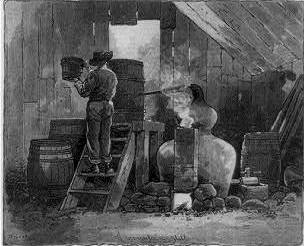
\includegraphics[width=.4\textwidth]{../pictures/moonshine.jpg}
\end{figure}

\subsubsection{Peering into Learning}

\noindent This is a quick introduction to the main ideas used in the rest of the
book. It provides a range of things to think about as you get started
with a new peer learning project, or as you use peeragogy to redesign
and reassess an existing collaboration. You'll probably want to read
this first and then do some reflection before diving into the other
parts of the book.

\subsubsection{Motivation}
You might wonder why we're doing this project -- what we hope to get
out of it as volunteers, and how we think what we're doing can make a
positive difference in the world. Have a look at this chapter if you,
too, are thinking about getting involved in peeragogy, or wondering
how peeragogy can help you accelerate your own learning projects.

\paragraph{Case Study: 5PH1NX}
We enjoy riddles with more than one answer, so we've included this
detailed narrative example of peeragogy in action near the beginning
of the book. We hope you are inspired by the challenge of doing
peeragogy in a school setting that is recounted here. Explore this
case study for ideas and encouragement for your own learning
adventures.

\subsubsection{Patterns, use cases, examples}

\noindent Here we show you some of the signposts that can serve as
both a key and compass to the kind of social problem solving that
happens in peeragogy projects. If you want some underlying components
to try out, mix and match these and experiment with peeragogy right
away. You come back to this chapter for a deeper understanding of the
processes we talk about later on. A detailed catalog of patterns and
anti-patterns that we've drawn from our own practice form a core part
of the book.

\subsubsection{Convening a Group}

\noindent You'll probably want to use this chapter to organize your thinking as
you start a new peeragogy project or think about how to apply peeragogy
ideas in an existing collaboration. A few clusters of simple but
important questions will inspire unique answers for you and your group.
We hope these mental frameworks are helpful to not only initiate
progress, but also to maintain momentum.

 \paragraph{Play \& Learning} What
makes learning fun? Just as actors learn their roles through the dynamic
process of performance, In other words, the more we engage with a topic,
the better we learn it and the more satisfying - or fun - the process
becomes.

\paragraph{K-12 Peeragogy} The key to becoming a successful
`connected educator-learner' involves spending the time needed to learn
how to learn and share in an open, connected environment. Once you make
the decision to enter into a dialogue with another user, you become a
connected educator/learner and tap into the power of networks to
distribute the load of learning. Depending on their age, you can even
facilitate an awareness of peer networks among your students.

\paragraph{P2P Self-Organizing Learning Environments} This conversational
section engages you in a journey through diverse points of entry that
interact with your physical learning space. Within this chapter of word
and picture images, the emerging structure and reciprocal mentoring that
may be inspired causes a ripple effect on those who open the door to its
possibilities.

\subsubsection{Organizing a Learning Context}

\noindent We talk about how peer learning is organized into ``courses'' and
``spaces'', again drawing on our experience in the peeragogy project. We
present the results of an informal poll that reveals some of the
positive and some of the negative features of our early choices.

\paragraph{Adding Structure with Activities} The first rule of thumb for
peer learning is: announce activities only when you plan to take part as
a fully engaged participant. Then ask a series of questions: what is the
goal, what makes it challenging, what worked in other situations, what
recipe is appropriate, what is different about learning about this
topic?

\paragraph{Student Authored Syllabus} Here's one place you might
explore to see ways in which freedom in student-directed learning
complements the structural needs for the content and group. Check this
out for various methods to welcome ambiguity and co-created curriculum
into your projects. You may want to start with one or two ideas in an
activity to transition into this format, yet embracing the risk on a
larger scale is fun as well.

\paragraph{Connectivism in Practice} Massive Open
Online Courses (MOOCs) are decentralized online learning experiences:
individuals and groups create blogs or wikis and comment on each
other's work, often with a focus on where to find information. A
course typically has a topic, activities, reading resources and a
guest speaker for each week. Items are tagged to allow for
aggregation. Links to technology resources are provided (such as
gRSShopper from Stephen Downes).

\paragraph{Case Study: Collaborative Explorations} You can try out this
chapter to encourage individuals pursuing their own interests in a
predetermined topic while at the same time influencing the learning of
the whole group by sharing and reflecting upon their findings. These
interactions of supportive mutual inquiry evolve the content and
structure within a short time frame and with open-ended results.

\subsubsection{Cooperation}

\noindent Sometimes omitting the figurehead empowers a
group. Co-facilitation tends to work in groups of people who gather to
share common problems and experiences. The chapter suggests how to
co-facilitate discussions, wiki workflows, and live
sessions. Conducting an ``after action review'' helps to avoid blind
spots.

\paragraph{The Workscape} In a corporate workscape, people are free-range
learners: protect the learning environment, provide nutrients for
growth, and let nature take its course. A workscape features profiles,
an activity stream, wikis, virtual meetings, blogs, bookmarks, mobile
access and a social network.

\paragraph{Participation} Participation grows from having a
community of people who learn together, using a curriculum as a starting
point to organize and trigger engagement. Keep in mind that
participation may follow the 90/9/1 principle (lurkers/editors/authors)
and that people may transition through these roles over time.

\paragraph{New Designs For Co-Working And Co-Learning} Designing for
peer learning requires a new approach.  A case study dealing focusing
on PlanetMath shows one way to go.

\subsubsection{Assessment}

\noindent Asking questions about assessment in the context of the
Handbook (Who needs to know? Based on what data? In what format?)
suggests ``usefulness'' (real problems solved) is an appropriate
metric. We use the idea of return on investment (the value of changes
in behavior divided by the cost of inducing the change) to assess the
peeragogy project itself, as one example.

\paragraph{Researching peeragogy} Three new patterns are introduced
(Frontend and Backend, Spanning Set, and Minimum Viable Project) which
form the basis of a ``meta-model'' that can be used to study and
design for peer learning.

\subsubsection{Technologies, Services, and Platforms}

\noindent Issues of utility, choice, coaching, impact and roles attach
to the wide variety of tools and technologies available for peer
learning. Keys to selection include the features you need, what people
are already using, and the type of tool (low threshold, wide wall,
high ceilings) used for collaboration.

\paragraph{Forums} Forums are web-based communication media
that enable groups of people to conduct organized multimedia discussions
about multiple topics over a period of time, asynchronously. A rubric
for evaluating forum posts highlights the value of drawing connections.
The chapter includes tips on selecting forum software.

\paragraph{Wiki} A
wiki is a website whose users can add, modify, or delete its content via
a web browser. Pages have a feature called ``history'' which allows
users to see previous versions and roll back to them. The chapter
includes tips on how to use a wiki and select a wiki engine, with
particular attention to peer learning opportunities.

 \paragraph{Real-time meetings} Web services enable broadband-connected
learners to communicate in real time via audio, video, slides,
whiteboards, chat, and screen-sharing. Possible roles for participants
in real-time meetings include searchers, contextualizers, summarizers,
lexicographers, mappers, and curators. This mode of interaction
supports emergent agendas.

\subsubsection{Resources}

\noindent Here we present several ways to get involved in peer
learning, including information about where to find the Peeragogy
project online, a sample syllabus with four actions bring peer
learning to life, tips on writing for The Handbook, and our Creative
Commons Zero 1.0 Universal (CC0 1.0) Public Domain Dedication.


\part{Peer Learning} \label{peer-learning-part} %%%%%%%%%%%%%%%%%%%%
%
\chapter[\textbf{An Overview}]{An Overview of Peer Learning}
%
This part of the book offers our most important insights into peer
learning. A number of earlier theories and experiments have focused on
various aspects of collaborative, connective, and shared, non-didactic
learning systems. There's a rumbling among several well-known thinkers
that when combined with new technologies, peer learning strategies could
have a big impact on the way educational institutions work in the
future. Our aim here is just to make the basic ideas concretely
understandable and immediately applicable. The best course is to try it
out and see how it works for you.

\begin{center}

\includegraphics[width=.4\textwidth]{../pictures/peeragogy-in-action.jpg}
\end{center}

Peeragogy is about peers learning together and helping each other learn.
The idea is that each person contributes to the group in their own way.
The contribution of each peeragogue depends on a healthy sense of
self-awareness. You ask yourself, ``What do I have to offer?'' and
``What do I get out of it?'' We think you'll come up with some exciting
answers to those questions!

Our first strategy for peer learning invites you to engage in a
self-assessment of your motivations. Here you take into account things
like the learning context, timing and sequence of learning activities,
social reinforcements, and visible reward. Our view is that learning is
most effective when it contains some form of enjoyment or satisfaction,
or when it leads to a concrete accomplishment.

Indeed, this is the kind of learning that you choose to do, whether
you're being ``trained'' or not. You're in charge! Furthermore, this
kind of learning is usually fun. Indeed, as we'll describe below, there
are deep links between play and learning. We believe we can improve the
co-learning experience by adopting a playful mindset. Certainly some of
our best learning moments in the~Peeragogy project have been peppered
with humor and banter.

Apart from self-assessment and playfulness, here are two key factors to
keep in mind:

\textbf{``Personal'' supports ``peer'':} We can consciously cultivate
living, growing, responsive webs of information, support, and
inspiration that help us be more effective learners. This is a
``personal learning network''.~We'll offer tips on how to build these
networks -- and we'll also explain how strong personal learning networks
can evolve into even stronger \emph{peer} learning networks.

\textbf{``Peer'' supports ``personal'':} As we work together to develop
shared plans or ``roadmaps'' for our collective efforts in group
projects, we usually can find places where we have something to offer,
and places where we have something to learn. Furthermore, if we are
willing to ask for some help and offer our help to others, then we can
really learn a lot! This is why building effective \emph{inter}personal
learning strategies should be part of your personal learning plan.

In the following sections, you can read some more about these
strategies, or you can skip ahead to
\href{http://peeragogy.org/peeragogy-in-action/}{Part III} to start
looking at techniques you can use to build your own peer learning group.

\subsection{Peer learning through the ages}

The new term, ``peeragogy,'' that we use in this book is a riff on the
word pedagogy --- the art, science, or profession of teaching. Pedagogy
has a somewhat problematic story of origin: it comes from the ancient
Greek tradition of having a child (paidos) be supervised (agogos) by a
slave. Greek philosophers disagreed with each other as to the best way
for individuals to gain knowledge (and even more so, wisdom). Socrates,
who insisted that he was not wise, also insisted that his interlocutors
join him in investigating truth claims, as peers. The most famous of
these interlocutors, Plato, on a more pedagogical bent, spoke of an
enlightened few, whose responsibility it was to show others the light of
knowledge (illustrated by his famous allegory of ``The Cave'').

In more recent centuries, various education theorists and reformers have
challenged the effectiveness of what had become the traditional
teacher-led model. Most famous of the early education reformers in the
United States was John Dewey, who advocated new experiential learning
techniques. In his 1916 book, \emph{Democracy and Education}{[}1{]},
Dewey wrote, ``Education is not an affair of `telling' and being told,
but an active and constructive process.'' Soviet psychologist Lev
Vygotsky, who developed the concept of the Zone of Proximal Development,
was another proponent of ``constructivist'' learning. His book,
\emph{Thought and Language}, also gives evidence to support
collaborative, socially meaningful, problem-solving activities over solo
exercises {[}2{]}.

Within the last few decades, things have begun to change very rapidly.
In \emph{Connectivism: A Learning Theory for the Digital Age}, George
Siemens argues that technology has changed the way we learn, explaining
how it tends to complicate or expose the limitations of the learning
theories of the past {[}3{]}. The crucial point of connectivism is that
the connections that make it possible for us to learn in the future are
more relevant than the sets of knowledge we know individually, in the
present. Furthermore, technology can to some degree and in certain
contexts, replace know-how with know-where-to-look.

If you want more details on the history, theories, and recent
experiments related to peer learning, we have a more extensive
\href{http://peeragogy.org/resources/literature-review-peeragogy/}{literature
review} available. We've also adapted it into
\href{http://en.wikipedia.org/wiki/Peer\_learning}{Wikipedia page},
which you can edit as well as read.

\begin{figure}
\href{http://commons.wikimedia.org/wiki/File:Platon\_Cave\_Sanraedam\_1604.jpg}{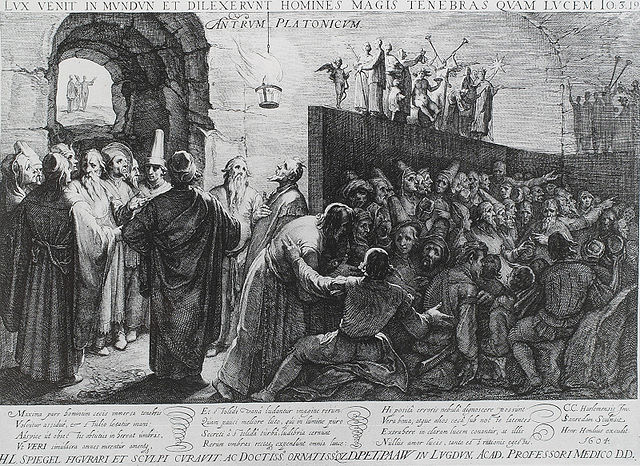
\includegraphics[width=\textwidth]{../pictures/plato_cave.jpg}}
 \caption{\href{http://commons.wikimedia.org/w/index.php?title=File:Platon\_Cave\_Sanraedam\_1604.jpg\&oldid=68567627}{Platon Cave Sanraedam (1604)}. By Jan Saenredam {[}Public domain{]}, via
 Wikimedia Commons}
\end{figure}

\subsection{What makes learning fun? (Or boring, as the case may be!)}

Individuals learn by doing in a continuous process. This is most
effective when it contains some form of enjoyment, satisfaction, or
accomplishment. So for each peer-learning participant, there's a simple
question: ''What makes learning fun for \emph{me}?''

\subsubsection{Two learning stories}

\begin{enumerate}
\item
  A study group for a tough class in neuropsychology convenes at at the
  library late one night, resolving to do well on the next day's exam.
  The students manage to deflect their purpose for a while by gossiping
  about college hook-ups and parties, studying for other classes, and
  sharing photos. Then, first one member, then another, takes the
  initiative and as a group, the students eventually pull their
  attention back to the task at hand. They endure the monotony of
  studying for several hours, and the next day, the exam is theirs.
\item
  A young skateboarder spends hours tweaking the mechanics of how to
  make a skateboard float in the air for a split second, enduring
  physical pain of repeated wipeouts. With repetition and success comes
  a deep understanding of the physics of the trick. That same student
  cannot string together more than five minutes of continuous attention
  during chemistry class and spends even less time on homework for the
  class before giving up.
\end{enumerate}

\subsection{Which is more fun, skateboarding or chemistry?}

Peer-learning participants succeed when they are motivated to learn.
Skateboarding is primarily intrinsically motivated, with some extrinsic
motivation coming from the respect that kids receive from peers when
they master a trick. In most cases, the primary motivation for learning
chemistry is extrinsic, coming from parents and society's expectations
that the student excel and assure his or her future by getting into a
top college.

The student very well could be intrinsically motivated to have a glowing
report card, but not for the joy of learning chemistry, but because of
the motivaton to earn a high grade as part of her overall portfolio.
Taken a different way, what is it about chemistry that's fun for a
student who \emph{does} love the science? Perhaps she anitcipates the
respect, power and prestige that comes from announcing a new
breakthrough; or Or, she may feel her work is important for the greater
good, or prosperity, of humanity; or~she may simply thrill to see atoms
bonding to form new compounds.

Learning situations frequently bore the learner when extrinsic
motivation is involved. Whether by parents or society, being forced to
do something, as opposed to choosing to, ends up making the individual
less likely to succeed. In some cases it's clear, but trying to figure
out what makes learning fun for a a group of individual humans can be
very difficult. Often there is no clear-cut answer that can be directly
applied in the learning environment. Either way, identifying the factors
that can make learning boring or fun is a good start. Perhaps learning
certain skills or topics is intrinsically boring, no matter what, and we
have to accept that.

\begin{figure}
\begin{center}
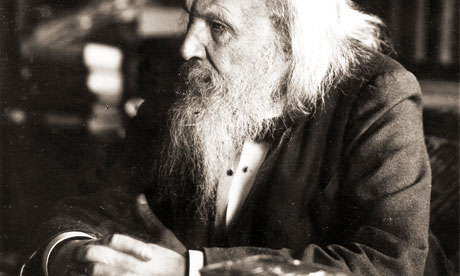
\includegraphics[width=.8\textwidth]{../pictures/mendeleev.jpg}
\caption{Photo of Dmitri Mendeleev (1834-1907). Found on The Guardian's \href{http://www.guardian.co.uk/science/blog/2011/dec/07/dmitri-mendeleev-business-card}{Notes \& Theories blog}. Public domain.}
\end{center}
\end{figure}


\subsubsection{Learning patterns}

One way to think about fun learning is that it's fun to learn new
patterns. Jürgen Schmidhuber wrote: ``A separate reinforcement learner
maximizes expected fun by finding or creating data that is better
compressible in some yet unknown but learnable way, such as jokes,
songs, paintings, or scientific observations obeying novel, unpublished
laws'' {[}4{]}. So the skateboarder enjoyed coming across new patterns
(novel tricks) that he was \emph{able} to learn; tricks that challenged
his current skill level.

\subsection{Learner, know thyself: A self-evaluation technique}

When joining the Peeragogy project, I did a brief self-evaluation about
what makes me turn on to learning:

\begin{itemize}
\item
  \emph{Context.} I resist being groomed for some unforseeable future
  rather than for a purpose.
\item
  \emph{Timing and sequence.}I find learning fun when I'm studying
  something as a way to procrastinate on another pressing assignment.
\item
  \emph{Social reinforcement.}Getting tips from peers on how to navigate
  a snowboard around moguls was more fun for me than my Dad showing me
  the proper way to buff the car's leather seats on chore day.
\item
  \emph{Visible reward}. In high school, it was not fun in the moment to
  sit and compose a 30-page reading journal for Frankenstein. But owing
  in part to those types of prior experiences, writing is now fun and
  it's a pleasure to learn how to write better.
\end{itemize}

\subsection{The role of metacognition in peer learning}

The profile of each individual participant, both from the perspective of
self-awareness, as well as from the perspective of maximal value of
contribution to the group endeavor, becomes a metacognitive inquiry into
each peeragogue's skills, talents, subject matter expertise,
socialization and suitability for the array of roles and positions
required to achieve a communally defined and framed goal or output.
``Metacognitive'' means that the peeragogue is practicing awareness of
how he or she is thinking and attending. The short form is
"\emph{Deliberate self-awareness of one's thinking processes}."

Since in principle there is no authority figure or leader to exercise
judgment or discretion regarding the above, it becomes a necessary
self-evaluative examination and declaration in regard to the group,
enabling participating individuals to maximize their engagement and
contribution to the undertaking.

\subsubsection{\textbf{Possible Roles}}

\begin{itemize}
\item
  Leader, Manager, Team Member, Worker
\item
  Content Creator, Author, Content Processor, Reviewer, Editor
\item
  Presentation Creator, Designer, Graphics, Applications
\item
  Planner, Project Manager, Coordinator, Attendee, Participant
\item
  Mediator, Moderator, Facilitator, Proponent, Advocate, Representative,
  Contributor
\end{itemize}

\subsubsection{\textbf{Possible Contributions}}

\begin{itemize}
\item
  Create, Originate, Research, Aggregate
\item
  Develop, Design, Integrate, Refine, Convert
\item
  Write, Edit, Layout
\end{itemize}

We find it useful to build in a brief pause at the commencement of the
project for each peeragogue to honestly self-define and declare to the
group what he thinks he can bring to the table as a function of his
knowledge, skills, capacities, and preferences. This process primes the
group for cohesion and success.

\subsection{Personal Learning Networks and Peer Learning Networks}

Personal Learning Networks are the collections of people and information
resources (and relationships with them) that people cultivate in order
to form their own learning networks --- living, growing, responsive
sources of information, support, and inspiration that support
self-learners.

\begin{quote}
\textbf{Howard Rheingold}:\emph{When I started using social media in the
classroom, I looked for and began to learn from more experienced
educators. First, I read and then tried to comment usefully on their
blog posts and tweets. When I began to understand who knew what in the
world of social media in education, I narrowed my focus to the most
knowledgeable and adventurous among them. I paid attention to the people
the savviest social media educators paid attention to. I added and
subtracted voices from my attention network, listened and followed, then
commented and opened conversations. When I found something I thought
would interest the friends and strangers I was learning from, I passed
along my own learning through my blogs and Twitterstream. I asked
questions, asked for help, and eventually started providing answers and
assistance to those who seemed to know less than I. The teachers I had
been learning from had a name for what I was doing --- ``growing a
personal learning network.'' So I started looking for and learning from
people who talked about HOW to grow a ``PLN'' as the enthusiasts called
them.}
\end{quote}

\subsubsection{\textbf{Strong and weak ties}}

Your PLN will have people and sites that you check on often -- your main
sources of information and learning -- your `strong ties'. Your `weak
ties' are those people and sites that you don't allow a lot of bandwidth
or time. But they may become strong over time, as your network grows or
your interests expand. This is a two-way street -- it is very important
that you are sharing what you learn and discover with those in your
network and not just taking, if you want to see your network expand.

\begin{center}
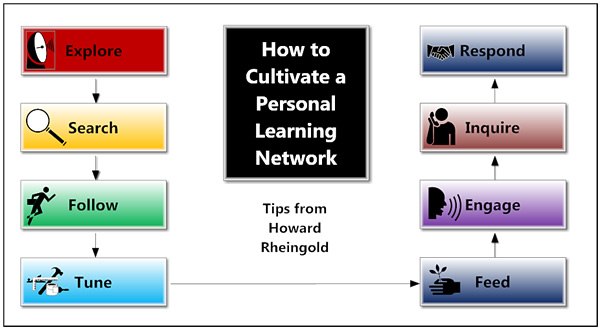
\includegraphics[width=.7\textwidth]{../pictures/Personal-Learning-Network-900px-v2.jpeg}
\end{center}

\subsubsection{Peer Learning Networks}

Later in the handbook we'll talk more about how to develop and share
``\href{http://peeragogy.org/patterns-usecases/patterns-and-heuristics/roadmap/}{peeragogical
profiles}'' -- in other words how to advertise what you want to learn,
and what you'd be interested in helping teach others. A network of
people who share their profiles and work together to
learn/teach/heal/communicate/etc. is a ``Peer Learning Network''. You'll
also find more information about building a PLN in our article on
\href{http://peeragogy.org/k-12-peeragogy/}{Peeragogy for K-12
Educators} (the article is also useful even if you're not formally
employed a teacher).

\subsection{Personal Learning Plans and Peer Learning Plans}

A PLP is designed to develop a learner's learning and teaching
capabilities. Learners learn how to develop, implement, review, and
adjust personal learning goals. The PLP supports learners in developing
knowledge and skills that will enable them to:

\begin{enumerate}
\item
  Identify appropriate future options;
\item
  Review their strengths and areas for development;
\item
  Identify goals and plans for improvement;
\item
  Monitor their actions and review and adjust plans as needed to achieve
  their goals.
\end{enumerate}

\subsubsection{\textbf{Steps in making the PLP}}

\begin{enumerate}
\item
  \emph{Learning needs:}What do you most need to learn about in the time
  ahead?
\item
  \emph{Learning activities:} What are the best ways you learn, what
  learning activities will meet your learning needs, what help will you
  need and how long will it take?
\item
  \emph{Evidence of learning:}What will you put into your personal
  portfolio to demonstrate your learning progress and achievements?
\end{enumerate}

\subsubsection{Peer Learning Plans}

On the same page where we talk about ``peeragogical profiles'', we also
talk about how to build a
"\href{http://peeragogy.org/patterns-usecases/patterns-and-heuristics/roadmap/}{shared
roadmap}'' for your peer learning project. Indeed, the idea of a
``roadmap'' is really a central pattern that comes up in this book again
and again.

\subsection{From training to learning}

\begin{figure}
\begin{center}
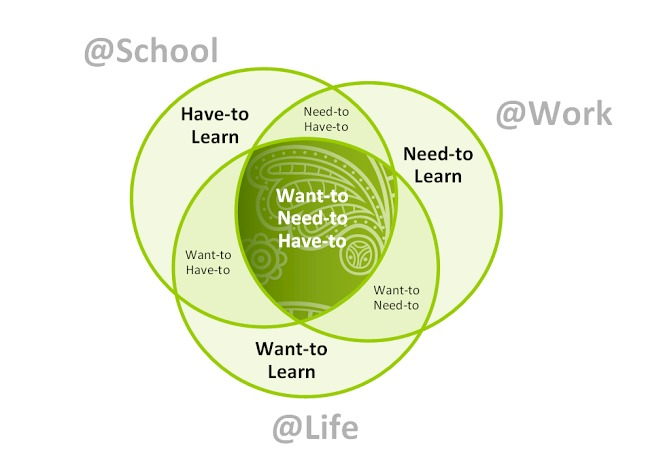
\includegraphics[width=.8\textwidth]{../pictures/learn.jpg}
\caption{``I think because of the tremendous changes we see in education and at
work, the sets (attitudes) are beginning to overlap more and more,''
said Joachim Stroh of the Google+ community, Visual Metaphors. (Used with permission)}
\end{center}
\end{figure}

The idea we develop here relates back to the question ``what makes
learning fun for me.'' In short, if it's not something that you choose,
it's not as likely to stick. However, dozen years ago, the words
\emph{training} and \emph{learning} were interchangeable, but today
\emph{learning} is revered and \emph{training} is in the dog house.
What's the difference? Training is something that's pushed on you;
someone else is in charge. Learning is something you choose to do,
whether you're being trained or not. You're in charge.

And think of all the people we learn from who aren't necessarily
trainers! Parents, grandparents, aunts, uncles, brothers, sisters,
playmates, cousins, Little Leaguers, Scouts, school chums, roommates,
teammates, classmates, study groups, coaches, bosses, mentors,
colleagues, gossips, co-workers, neighbors, and our kids\ldots{}

\emph{This has ramifications for the way people manage}. To extract
optimal performance from workers, managers must inspire them rather than
command them. Antoine de Saint-Exupéry put it nicely: ``If you want to
build a boat, do not instruct the men to saw wood, stitch the sails,
prepare the tools and organize the work, but make them long for setting
sail and travel to distant lands.'' Knowledge workers of the future will
have instant, ubiquitous access to the Net. The measure of their
learning is an open-book exam. ``What do you know?'' is replaced with
``What can you do?''.

\begin{quote}
\textbf{Jay Cross}: If I were an instructional designer in a moribund
training department, I'd polish up my resume and head over to marketing.
Co-learning can differentiate services, increase product usage,
strengthen customer relationships, and reduce the cost of hand-holding.
It's cheaper and more useful than advertising. But instead of just
making a copy of today's boring educational practices, build something
based on interaction and camaraderie, perhaps with some healthy
competition thrown in. Again, the emphasis should always be on learning
in order to do something!
\end{quote}

\subsection{Play and learning}

Once more we're back to the question, ``What makes learning fun?'' There
are deep links between play and learning. Consider, for instance, the
way we learn the rules of a game through playing it. The first times we
play a card game, or a physical sport, or a computer simulation we test
out rule boundaries as well as our understanding. Actors and
role-players learn their roles through the dynamic process of
performance. The resulting learning isn't absorbed all at once, but
accretes over time through an emergent process, one unfolding further
through iterations. In other words, the more we play a game, the more we
learn it.

In addition to the rules of play, we learn about the subject which play
represents, be it a strategy game (chess, for example) or simulation of
economic conflict. Good games echo good teaching practice, too, in that
they structure a single player's experience to fit their regime of
competence (cf. Vygotsky's zone of proximal learning, a la Gee {[}5{]}).
That is to say a game challenges players at a level suited to their
skill and knowledge: comfortable enough that play is possible, but so
challenging as to avoid boredom, eliciting player growth. Role-playing
in theater lets performers explore and test out concepts; see Boal
{[}6{]}. Further, adopting a playful attitude helps individuals meet new
challenges with curiousity, along with a readiness to mobilize ideas and
practical knowledge. Indeed, the energy activated by play can take a
person beyond an event's formal limitations, as players can assume that
play can go on and on {[}7{]}.

\begin{quote}
\textbf{Douglas Thomas and John Seely Brown}: ``All systems of play are,
at base, learning systems.'' {[}8{]}
\end{quote}

Games have always had a major social component, and learning plays a key
role in that interpersonal function. Using games to build group cohesion
is an old practice, actually a triusm in team sports.

It is important to locate our peeragogical moment in a world where
gaming is undergoing a renaissance. Not only has digital gaming become a
large industry, but gaming has begun to infiltrate non-gaming aspects of
the world, sometimes referred to as ``gamification.'' Putting all three
of these levels together, we see that we can possibly improve
co-learning by adopting a playful mindset. Such a playful attitude can
then mobilize any or all of the above advantages. For example,

\begin{itemize}
\item
  Two friends are learning the Russian language together. They invent a
  vocabulary game: one identifies an object in the world, and the other
  must name it in Russian. They take turns, each challenging the other,
  building up their common knowledge.
\item
  A middle-aged man decides to take up hiking. The prospect is somewhat
  daunting, since he's a very proud person and is easily stymied by
  learning something from scratch. So he adopts a ``trail name'', a
  playful pseudonym. This new identity lets him set-aside his
  self-importance and risk making mistakes. Gradually he grows
  comfortable with what his new persona learns.
\item
  We can also consider the \textbf{design} field as a useful kind of
  playful peeragogy. The person \emph{playing the role} of the designer
  can select the contextual frame within which the design is performed.
  This frame can be seen as the \emph{rules} governing the design, the
  artifact and the process. These rules, as with some games, may change
  over time. Therefore the possibility to adapt, to tailor one's
  activities to changing context is important when designing playful
  learning activities. (And we'll look at some ways to design peer
  learning experiences next!)
\end{itemize}

\subsection{From Peer Learning to ``Peeragogy''}

The idea that we needed a new theory (which we called \emph{paragogy})
arose out of the challenges we faced doing peer learning. Specifically,
we were particularly interested in the conditions that were required for
volunteer contributors to drive an learning-focused organization's
agenda, and improve things for participating learners and teachers. How
could the organization itself ``learn'' and grow, while participants
were also learning and becoming better contributors?

As this idea took form, we reflected more on how learning and
organizations work. Just like it would be rare for a business to be
successful if it does not take into account the needs and interests of
its clients, it is unlikely for a learning project to be successful if
the act of learning is not somehow relevant for the people doing it.

So, paragogy became \emph{a set of proposed principles} for
understanding learning (and working) together. In particular, we focused
on the way in which co-learners shape their learning context together.
Paragogy is not a recipe: its ideas can grow and change to suit the
needs of the moment; as it has matured, it has become more of an
``approach'' than it is a set of set-in-stone principles. It's also riff
on the word ``andragogy'', which comes from Malcolm Knowles. He wrote:

\begin{quote}
\emph{{[}A{]}ndragogy is simply another model of assumptions about adult
learners to be used alongside the pedagogical model of assumptions,
thereby providing two alternative models for testing out the assumptions
as to their `fit' with particular situations. Furthermore, the models
are probably most useful when seen not as dichotomous but rather as two
ends of a spectrum , with a realistic assumption (about learners) in a
given situation falling in between the two ends} {[}9{]} (p. 43).
\end{quote}

We also tried, at least at first, to be similarly non-oppositional with
respect to andragogy:

\begin{quote}
\emph{{[}T{]}he most important initial condition in andragogy seems to
be that an adult educator or facilitator is part of the picture. In a
peer-based setting, that may not be the case: we can easily find
examples of learning environments where there is no ``teacher'' in the
``classroom''; where, for example, the task of facilitation is shared
among all participants or even encoded in the learning materials or
supportive technologies. Not that one way is more desirable than
another: we simply mean to highlight the fact that the most basic
features of a given learning environment will influence everything
else.} {[}10{]}
\end{quote}

``Paragogy'' is intended to be a broad, inclusive, and purposefully
ambiguous term. ``Peeragogy'' by contrast attempts to make the idea more
concrete and immediately understandable: peeragogy is about peers
learning together, and teaching each other. In the end, the two words
are actually synonyms. If you prefer to go merrily into theory-building
mode, feel free to spell it ``paragogy''. If you want to be a bit more
down to earth, use ``peeragogy.''

\subsubsection{Different ways to analyze the learning process}

Since we are interested in how students (and others) can collaborate in
learning, bringing to their own particular experiences, strengths, and
weaknesses to bear, we ask: ``How can each participant contribute to a
group in their own way? Which kind of activities can we design to foster
``multi-modal'' collaborative learning, and how do we assess the
outcomes?'' One approach is to look at the ``multiple different social
roles'' which people take on in educational contexts:

\begin{quote}
\emph{{[}W{]}e use {[}Ken{]} Wilber's terms to describe a given social
role in terms of its constituent actions. So for example, the role of
``being a student'' might be described as follows: ``\textbf{I}}\emph{go
to class, \textbf{we}}\emph{do a class project, the objects of concern
(``\textbf{Its}}\emph{'') are things I can add to my portfolio or
work-record; and fundamentally, \textbf{it}}\emph{is all about gaining a
skill.'' This simple background story gives us a notion of role,
persona, or identity: a role that is defined by its constituent actions,
relative a given social context. And here, context is conceived of,
after Nishida, as a ``shared context in motion.''} {[}11{]}
\end{quote}

After doing some personal reflection on the roles you want to take on
and the contributions you want to make (as we discussed above), you may
also want to work together with your learning group to analyze the
learning process in more detail. There are many different phases,
stages, and dimensions that you can use to help structure and understand
the learning experience: we list some of these below.

\begin{itemize}
\item
  \emph{Guidance \& Support}, \emph{Communication \& Collaboration},
  \emph{Reflection \& Demonstration}, \emph{Content \& Activities} (from
  Gráinne Conole)
\item
  \emph{Forming}, \emph{Norming}, \emph{Storming}, \emph{Performing}
  from Bruce Tuckman.
\item
  The ``five-stage e-moderating model'' from GIlly Salmon
\item
  \emph{Assimilative, Information Processing, Communicative, Productive,
  Experiential, Adaptive}(from Oliver and Conole)
\item
  Multiple intelligences (after Howard Gardner).
\item
  The associated ``mental state''(after Csíkszentmihályi; see
  picture)\emph{}
\item
  Considered in terms of ``Learning Power'' (Deakin-Crick, Broadfoot,
  and Claxton).
\end{itemize}

\begin{figure}
\begin{center}
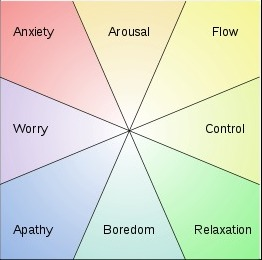
\includegraphics[width=.5\textwidth]{../pictures/challenge.jpg} 
\end{center}
\caption{
\href{http://commons.wikimedia.org/wiki/File\%3AChallenge\_vs\_skill.svg}{Challenge vs. Skill}. By w:User:Oliverbeatson (w:File:Challenge vs skill.jpg)
{[}Public domain{]}}
\end{figure}

\subsection{Further reading}

\subsubsection{A word list for your inner edu-geek}

\begin{itemize}
\item
  Constructivism
\item
  Social constructivism
\item
  Radical constructivism
\item
  Enactivism
\item
  Constructionism
\item
  Connectivism
\end{itemize}

\subsubsection{On fun and boredom}

\begin{itemize}
\item
  \emph{The Contribution of Judo to Education} by Kano Jigoro
\item
  \emph{Pale King}, unfinished novel by David Foster Wallace,
\end{itemize}

\subsubsection{On Paragogy}

\begin{itemize}
\item
  Joe Corneli's
  ``\href{http://en.wikiversity.org/wiki/User:Arided/ImplementingParagogy}{Implementing
  Paragogy}'' lesson plan, on Wikiversity
\item
  Joe Corneli and Charlie Danoff's ``Paragogy Papers'', on
  \href{paragogy.net}{paragogy.net}
\end{itemize}

\subsubsection{on Learning vs Training}

\begin{itemize}
\item
  Hart, Jane.
  \href{http://www.c4lpt.co.uk/blog/2012/04/20/is-it-time-for-a-byol-bring-your-own-learning-strategy-in-your-organization-byol/}{Is
  it time for a BYOL (Bring Your Own Learning) strategy for your
  organization}?
\end{itemize}

\subsubsection{on PLNs}

\begin{itemize}
\item
  \href{http://dmlcentral.net/blog/howard-rheingold/shelly-terrell-global-netweaver-curator-pln-builder}{Shelly
  Terrell: Global Netweaver, Curator, PLN Builder}, blog post, with
  video
\item
  Will Richardson and Rob Mancabelli,
  \href{http://weblogg-ed.com/2011/personal-learning-networks-an-excerpt/}{Personal
  Learning Networks: Using the Power of Connection to Transform
  Education}
\item
  \href{http://delicious.com/hrheingold/pln}{Howard Rheingold's PLN
  links on Delicious}
\end{itemize}

\subsubsection{Exercises to help cultivate a playful attitude}

\begin{itemize}
\item
  Use the \href{http://www.rtqe.net/ObliqueStrategies/}{Oblique
  Strategies} card deck (Brian Eno and Peter Schmidt, 1st edition 1975,
  now available in its fifth edition) to spur playful creativity. Each
  card advises players to change their creative process, often in
  surprising directions.
\item
  Take turns making and sharing videos. This online collaborative
  continuous video storytelling involves a group of people creating
  short videos, uploading them to YouTube, then making playlists of
  results. Similar to \href{http://clipkino.info/}{Clip Kino}, only
  online.
\item
  Engage in theater play using Google+ Hangout. e.g. coming together
  with a group of people online and performing theatrical performances
  on a shared topic that are recorded.
\end{itemize}

\subsection{References}

\begin{enumerate}
\item
  Dewey, J. (2004). \emph{Democracy and education}. Dover Publications.
\item
  Vygotsky, L. S. (1986). \emph{Thought and language}. MIT press.
\item
  Siemens, G. (2005). Connectivism: A learning theory for the digital
  age. \emph{International Journal of Instructional Technology and
  Distance Learning}, 2(1), 3-10.
\item
  Schmidhuber, J. (2010). Formal theory of creativity, fun, and
  intrinsic motivation. \emph{Autonomous Mental Development (IEEE)},
  2(3), 230-247.
\item
  Gee, J. P. (1992). \emph{The social mind: Language, ideology, and
  social practice}. Series in language and ideology. New York: Bergin \&
  Garvey.
\item
  Boal, A. (1979). \emph{Theatre of the oppressed}. 3rd ed. London:
  Pluto Press.
\item
  Bereiter, C. and Scadamalia, M. (1993). \emph{Surpassing ourselves,
  an~inquiry into the nature and implications of expertise}. Peru,
  Illinois:~Open Court.
\item
  Douglas Thomas and John Seely Brown (2011), \emph{A New Culture of
  Learning: Cultivating the Imagination for a World of Constant Change}.
  CreateSpace.
\item
  Knowles, M. S. (1980). The modern practice of adult education: From
  pedagogy to andragogy. Chicago: Follett.
\item
  Corneli, J. and Danoff, C.J. (2011), Paragogy: Synergizing individual
  and organizational learning. (Published
  \href{\%20http://en.wikiversity.org/wiki/User:Arided/ParagogyPaper}{on
  Wikiversity}.)
\item
  Corneli, J., \& Mikroyannidis, A. (2012). Crowdsourcing education on
  the Web: a role-based analysis of online learning communities, in
  Alexandra Okada, Teresa Conolly, and Peter Scott (eds.),
  \emph{Collaborative Learning 2.0: Open Educational Resources}, IGI
  Global.
\end{enumerate}

~

%
\section*{Which is more fun, skateboarding or physics?}
Consider the following learning scenarios:

\begin{enumerate}
\itemsep1pt\parskip0pt\parsep0pt
\item
  A small study group for a tough class in Quantum Mechanics convenes at
  at the library late one night, resolving to do well on the next day's
  exam. The students manage to deflect their purpose for a while by
  gossiping about hook-ups and parties, studying for other classes, and
  sharing photos. Then, first one member, then another, takes the
  initiative and as a group, the students eventually pull their
  attention back to the task at hand. They endure the monotony of
  studying for several hours, and the next day, they own the exam.
\item
  A young skateboarder spends hours tweaking the mechanics of how to
  make a skateboard float in the air for a split second, enduring
  physical pain of repeated wipeouts. With repetition and success comes
  a deep understanding of the physics of the trick. That same student
  cannot string together more than five minutes of continuous attention
  during class and spends even less time on homework for the class
  before giving up.
\end{enumerate}

Peer-learning participants succeed when they are motivated to learn.
Skateboarding is primarily intrinsically motivated, with some extrinsic
motivation coming from the respect that kids receive from peers when
they master a trick. In most cases, the primary motivation for learning
physics is extrinsic, coming from parents' and society's expectations
that the student excel and assure his or her future by getting into a
top college.

The student very well could be intrinsically motivated to have a glowing
report card, but not for the joy of learning physics or chemistry, but
because of the motivation to earn a high grade as part of her overall
portfolio. Taken a different way, what is it about these topics that's
fun for a student who loves science? Perhaps she anticipates the
respect, power and prestige that comes from announcing a new
breakthrough; or she may feel her work is important for the greater
good, or prosperity, of humanity; or she may simply be thrilled to think
about atoms bonding to form new compounds.

Learning situations frequently bore the learner when extrinsic
motivation is involved. Whether by parents or society, being forced to
do something, as opposed to choosing to, ends up making the individual
less likely to succeed. In some cases it's clear, but trying to figure
out what makes learning fun for a group of individual humans can be very
difficult. Often there is no clear-cut answer that can be directly
applied in the learning environment. Either way, identifying the factors
that can make learning boring or fun is a good start. Perhaps learning
certain skills or topics is intrinsically boring, no matter what, and we
have to accept that.

{[}caption id=``'' align=``aligncenter''
width=``300''{]}\includegraphics{http://24.media.tumblr.com/tumblr_m25ta0G1pC1rttc8xo1_r1_500.jpg}
Photo of Dmitri Mendeleev (1834-1907). Found on The Guardian's Notes \&
Theories blog. Public domain.{[}/caption{]}

One way to think about fun learning is that it's fun to learn - and be
aware that you're learning - new patterns. Jürgen Schmidhuber wrote: ``A
{[}\ldots{}{]} learner maximizes expected fun by finding or creating
data that is better compressible in some yet unknown but learnable way,
such as jokes, songs, paintings, or scientific observations obeying
novel, unpublished laws'' {[}1{]}. So the skateboarder enjoyed coming
across new patterns: novel tricks that are learnable.~ (By the way, a
few people, like mathematician William Stein, find ways to combine the
love of science and skateboarding.)

\subsection{Learner, know thyself: a self-evaluation technique}

The learning contributed and acquired by each member of the peer
learning enterprise depends on a healthy sense of self-awareness. When
you ask yourself, ``What do I have to offer?'' and ``What do I get out
of it?'' we think you'll come up with some exciting answers. In peer
learning, whether or not you're pursuing a practical objective, you're
in charge, and this kind of learning is usually fun. Indeed, as we'll
describe below, there are deep links between play and learning. We
believe we can improve the co-learning experience by adopting a playful
mindset. Certainly some of our best learning moments in the Peeragogy
project have been peppered with humor and banter. So we found that a key
strategy for successful peer learning is to engage in a self-assessment
of your motivations and abilities. In this exercise, you take into
account factors like the learning context, timing and sequence of
learning activities, social reinforcements, and visible reward. The
peeragogical view is that learning is most effective when it contains
some form of enjoyment or satisfaction, or when it leads to a concrete
accomplishment.

When joining the Peeragogy project, Charles Jeffrey Danoff did a brief
self-evaluation about what makes him interested in learning:

\begin{enumerate}
\itemsep1pt\parskip0pt\parsep0pt
\item
  \textbf{Context}. I resist being groomed for some unforeseeable future
  rather than for a specific purpose.
\item
  \textbf{Timing and sequence}. I find learning fun when I'm studying
  something as a way to procrastinate on another pressing assignment.
\item
  \textbf{Social reinforcement}. Getting tips from peers on how to
  navigate a snowboard around moguls was more fun for me than my Dad
  showing me the proper way to buff the car's leather seats on chore
  day.
\item
  \textbf{Experiential awareness}. In high school, it was not fun to sit
  and compose a 30-page reading journal for Frankenstein. But owing in
  part to those types of prior experiences, I now find writing
  pleasurable and it's fun to learn how to write better.
\end{enumerate}

We will explore the patterns of peer learning in more detail in the
section on \href{http://peeragogy.org/practice/}{practice}.

\subsection{Reference}

\begin{enumerate}
\itemsep1pt\parskip0pt\parsep0pt
\item
  Schmidhuber, J. (2010). Formal theory of creativity, fun, and
  intrinsic motivation. Autonomous Mental Development (IEEE), 2(3),
  230-247.
\end{enumerate}

%
\section*{What kind of help do you need?}
Personal Learning Networks are the collections of people and information
resources (and relationships with them) that people cultivate in order
to form their own public or private learning networks --- living,
growing, responsive sources of information, support, and inspiration
that support self-learners.

\begin{quote}
\textbf{Howard Rheingold}: ``When I started using social media in the
classroom, I looked for and began to learn from more experienced
educators. First, I read and then tried to comment usefully on their
blog posts and tweets. When I began to understand who knew what in the
world of social media in education, I narrowed my focus to the most
knowledgeable and adventurous among them. I paid attention to the people
the savviest social media educators paid attention to. I added and
subtracted voices from my attention network, listened and followed, then
commented and opened conversations. When I found something I thought
would interest the friends and strangers I was learning from, I passed
along my own learning through my blogs and Twitter stream. I asked
questions, asked for help, and eventually started providing answers and
assistance to those who seemed to know less than I. The teachers I had
been learning from had a name for what I was doing --- ``growing a
personal learning network.'' So I started looking for and learning from
people who talked about HOW to grow a ``PLN'' as the enthusiasts called
them.''
\end{quote}

\subsubsection{Strong and weak ties}

Your PLN will have people and sites that you check on often -- your main
sources of information and learning -- your `strong ties'. Your `weak
ties' are those people and sites that you don't allow a lot of bandwidth
or time. But they may become strong later, as your network grows or your
interests expand. This is a two-way street -- it is very important that
you are sharing what you learn and discover with those in your network
and not just taking, if you want to see your network expand.

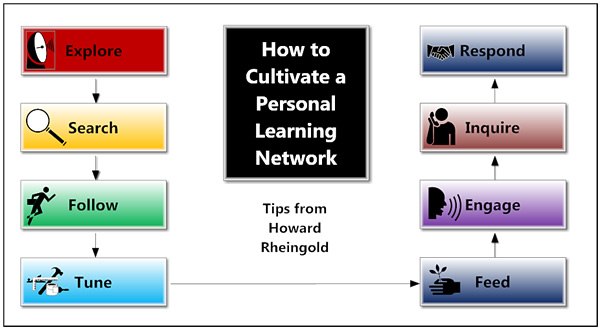
\includegraphics{http://peeragogy.org/wp-content/uploads/2013/09/cultivate.jpeg}

\subsubsection{Peer learning networks}

As you convene your peer learning group, in one form or another you will
develop and share ``peeragogical profiles'' --- advertising what you
want to learn, what you'd be interested in helping teach others. If you
present yourself and your projects in a thoughtful and engaging way,
this will help you to build effective connections. Networks of these
connections can span across different subjects, across a city, or across
national boundaries.~ Peeragogy helps to make sense of the idea of
``learning networks'' that has been around since at least the 1970s.~
Much as theories of pedagogy would be relevant for anyone carefully
planning an individual learning programme, peeragogy is relevant for
self-organized learning communities operating at larger scales.

%
\section*{How should we structure things?}
\subsection{From syllabus and curriculum to personal and peer learning
plans}

Part of the reason for the effectiveness of peeragogy is that the
``syllabus'' or ``curriculum'' -- more generally, the learning plan --
is developed by the people doing the learning. You won't faint with
shock when you see the reading list if you helped write it.

Having youwn own learning plan at the outset helps each participant
identify his or her unique learning and teaching proclivities and
capabilities, and effectively apply them in the peer setting. In
developing your personal plan, you can ask yourself the following
questions:

\begin{enumerate}
\item
  What do I most need to learn about in the time ahead?
\item
  What are the best ways I learn, what learning activities will meet my
  learning needs, what help will I need and how long will it take?
\item
  What will I put into my personal portfolio to demonstrate my learning
  progress and achievements?
\end{enumerate}
Early in the process, the peer learning group should also convene to
develop a peer learning plan. In the Peeragogy project, we used live
meetings and forum-style platforms to discuss the group-level versions
of the questions listed above. Personal learning needs and skills were
also aired via these platforms, but the key shared outcome was an
initial project plan. Initially this took the form of an outline of
handbook chapters to write, as well as a division of labor.

Nothing was set in stone, and both the peer group and individual
participants have continued to develop, implement, review, and adjust
their goals as the project develops. We have stayed sufficiently
connected to the original goal of producing a handbook about peer
learning that you now have one in your hands (or on your screen). We've
also added some new goals for the project as time has gone by. Having a
malleable framework enables peer learners to:

\begin{enumerate}
\item
  Identify appropriate directions and goals for future learning;
\item
  Review their strengths and areas for development;
\item
  Identify goals and plans for improvement;
\item
  Monitor their actions and review and adjust plans as needed to achieve
  their goals;
\item
  Update the goals to correspond to progress.
\end{enumerate}
This doesn't mean you have to let chaos rule, but often in the swirl of
ideas and contributions, new directions take shape and new ideas take
hold.

\subsubsection{Self-generating templates}

Documentation like mind maps, outlines, blogs or journals, and forum
posts for a peer learning project can create an audit trail or living
history of the process. You can mine the documentation of a past
peer-learning project or a completed phase of an ongoing project for
effective learning patterns, and if you're careful to document
everything, you can really benefit by taking the time to compare what
you've achieved against the stated goal or mission at the outset. Use
the record to reflect and evaluate key elements of the process for you
as a facilitator and as a member of the peer learning group. Adapt your
next phase of planning accordingly.

\subsection{From corporate training to learning on the job}

\begin{figure}
\begin{center}
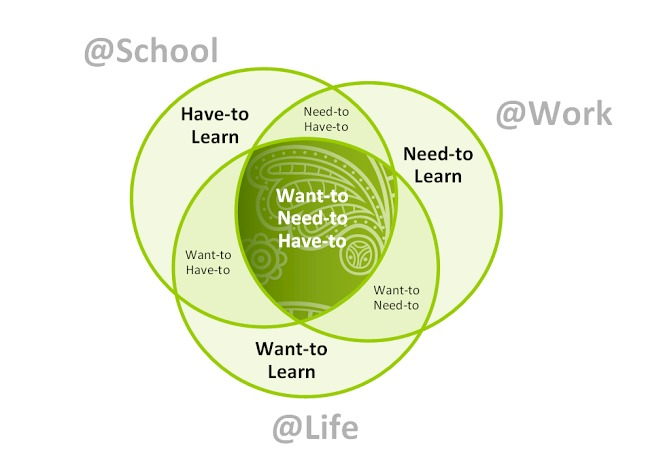
\includegraphics[width=.75\textwidth]{../pictures/learn.jpg}
\caption*{``I think because of the
tremendous changes we see in education and at work, the sets
(attitudes) are beginning to overlap more and more,'' said Joachim
Stroh of the Google+ community, Visual Metaphors.}
\end{center}
\end{figure}

Today's knowledge workers typically have instant, ubiquitous access to
the internet. The measure of their ability is an open-book exam. ``What
do you know?'' is replaced with ``What can you do?'' And if they get
bored, they can relatively easily be mentally elsewhere.

This has ramifications for the way managers manage as well as the way
teachers teach. To extract optimal performance from workers, managers
must inspire them rather than command them. Antoine de Saint-Exupéry put
it nicely: ``If you want to build a boat, do not instruct the men to saw
wood, stitch the sails, prepare the tools and organize the work, but
make them long for setting sail and travel to distant lands.''

\begin{quote}
\textbf{Jay Cross}: ``If I were an instructional designer in a moribund
training department, I'd polish up my resume and head over to marketing.
Co-learning can differentiate services, increase product usage,
strengthen customer relationships, and reduce the cost of hand-holding.
It's cheaper and more useful than advertising. But instead of just
making a copy of today's boring educational practices, build something
based on interaction and camaraderie, perhaps with some healthy
competition thrown in. Again, the emphasis should always be on learning
in order to do something!''
\end{quote}
In the section on \href{http://peeragogy.org/organize/}{organizing a
learning context}, we'll say quite a bit more about the implications
that our full conception of peer learning has for managers, teachers,
and other facilitators.

%
\section*{Can we work together on this?}
\subsection{Metacognition and mindfulness in peer learning}

Metacognition and mindfulness have to do with your awareness how how you
think, talk, participate, and attend to circumstances. It can be
particularly useful to apply this sort of ``meta awareness'' as you
think about the roles that you take on in a given project, the kind of
contributions you want to make, and what you hope to get out of the
experience. These are all likely to change as time passes, so it's good
to get in the habit of reflection.

\subsubsection{Potential roles in your peer-learning project}

\begin{enumerate}
\item
  Leader, Manager, Team Member, Worker
\item
  Content Creator, Author, Content Processor, Reviewer, Editor
\item
  Presentation Creator, Designer, Graphics, Applications
\item
  Planner, Project Manager, Coordinator, Attendee, Participant
\item
  Mediator, Moderator, Facilitator, Proponent, Advocate, Representative,
  Contributor
\end{enumerate}
\subsubsection{Potential contributions}

\begin{enumerate}
\item
  Create, Originate, Research, Aggregate
\item
  Develop, Design, Integrate, Refine, Convert
\item
  Write, Edit, Format
\end{enumerate}
\subsubsection{Potential motivations}

\begin{enumerate}
\item
  Acquisition of training or support in a topic or field;
\item
  Building relationships with interesting people;
\item
  Finding professional opportunities through other participants;
\item
  Creating or bolstering a personal network;
\item
  More organized and rational thinking through dialog and debate;
\item
  Feedback about performance and understanding of the topic.
\end{enumerate}
The process of shared reflection can prime a group for cohesion and
success. It can be tremendously useful to think about the motivations of
other participants, and how these can be jointly served. How can we
re-use the ``side-effects'' of individual and cooperative efforts in a
useful way?

\begin{figure}
\begin{center}

\includegraphics[width=.8\textwidth]{../pictures/sengai.jpg}
\end{center}
\caption*{A famous work in ink by Sengai Gibon (1750--1837)}
\end{figure}

\subsubsection{Two theories of motivation}

One of the most prominent thinkers working in the field of
(self-)motivation is Daniel Pink {[}1{]}, who proposes a theory of
motivation based on autonomy, mastery, and purpose, or, more colorfully:

\begin{enumerate}
\item
  The urge to direct my life
\item
  The desire to get better at something that matters
\item
  The yearning to do something that serves a purpose bigger than just
  ``myself''
\end{enumerate}
There's clearly a ``learning orientation'' behind the second point: it's
not just a matter of ``fun'' --- the sense of achievement matters. But
fun remains relevant. Thomas Malone {[}2{]} specifically asked ``What
makes things fun to learn?'' His proposed framework for building fun
learning activities is also based on the three ingredients: fantasy,
challenge, and curiosity.

We can easily see how ``participation'' relates to ``motivation'' as
described above. When I can get useful information from other people, I
can direct my own life better. When I have means of exploring my dreams
by chatting then over and exploring some of the elements in a safe way,
I'm in a much better position to make something in reality. A solid
reputation that comes from being able to help others serves as a good
indicator of personal progress, a sign that one is able to deal with
greater challenges. Relationships provide the most basic sense of being
part of something bigger than oneself: et cetera. We'll say more about
these matters in the chapters on
\href{http://peeragogy.org/cowork/}{Cooperation}.

\subsection{References}

\begin{enumerate}
\item
  Pink, D. (2011), Drive: The Surprising Truth About What Motivates Us,
  Canongate Books Ltd
\item
  Malone, T.W. (1981), Toward a Theory of Intrinsically Motivating
  Instruction, Cognitive Science, 4, pp. 333-369
\end{enumerate}

%
\section*{How do we know if we've won?}
\subsubsection{Different ways to analyze the learning process}

After doing some personal reflection on the roles you want to take on
and the contributions you want to make (as we discussed above), you may
also want to work together with your learning group to analyze the
learning process in more detail. There are many different phases,
stages, and dimensions - some simple and intuitive, others more complex
-- that you can use to help structure and understand the learning
experience: we list some of these below. (Detailed references are
collected in the recommended readings at the end of the book.)

\begin{enumerate}
\itemsep1pt\parskip0pt\parsep0pt
\item
  Forming, Norming, Storming, Performing (from Bruce Tuckman)
\item
  The ``five-stage e-moderating model'' (from Gilly Salmon)
\item
  I, We, Its, It (from Ken Wilber -- for an application in modeling
  educational systems, see {[}1{]})
\item
  Assimilative, Information Processing, Communicative, Productive,
  Experiential, Adaptive (from Martin Oliver and Gráinne Conole)
\item
  Guidance \& Support, Communication \& Collaboration, Reflection \&
  Demonstration, Content \& Activities (from Gráinne Conole)
\item
  Considered in terms of ``Learning Power'' (Ruth Deakin-Crick \emph{et
  al}.)
\item
  Multiple intelligences (after Howard Gardner)
\item
  The associated ``mental state'' (after Mihaly Csíkszentmihályi; see
  picture)
\end{enumerate}

{[}caption id=``'' align=``aligncenter''
width=``300''{]}\href{http://commons.wikimedia.org/wiki/File\%3AChallenge_vs_skill.svg}{\includegraphics{http://upload.wikimedia.org/wikipedia/commons/thumb/f/f6/Challenge_vs_skill.svg/300px-Challenge_vs_skill.svg.png}}
\href{http://commons.wikimedia.org/wiki/File\%3AChallenge_vs_skill.svg}{Challenge
vs. Skill}. By w:User:Oliverbeatson (w:File:Challenge vs skill.jpg)
{[}Public domain{]}, via Wikimedia Commons{[}/caption{]}

\subsubsection{Peer learning for one}

Can you apply the ideas of peer learning on your own? In a certain
sense, it's impossible, but somehow that never stops people from trying.
We find a striking parallel between the paragogy principles and the 5
Elements of Effective Thinking proposed by Edward Burger and Michael
Starbird in a recent book {[}2{]}. It's a nice short book and worth a
read. Here, we will just quote the titles of the main chapters:

\begin{enumerate}
\itemsep1pt\parskip0pt\parsep0pt
\item
  Quintessence, Engaging Change: Transform Yourself
\item
  Earth, Grounding Your Thinking: Understanding Deeply
\item
  Air, Creating Questions out of Thin Air: Be your own Socrates
\item
  Water, Seeing the Flow of Ideas: Look Back, Look Forward
\item
  Fire, Igniting Insights through Mistakes: Fail to Succeed
\end{enumerate}

We think that ``thinking'' is often most effective when it's done with
others, and this is something that Burger and Starbird don't give much
attention. Nevertheless, even when you find yourself on your own in the
midst of that challenging DIY project, you can use the techniques of
peer learning to understand yourself as a growing, changing part of a
shared context in motion. This can contribute to an effective and
adaptive outlook on life.

We invite you to approach this book as a ``peer learner'' -- and we hope
the techniques we've introduced here will serve you well in the world at
large.~~ The book, in part, documents the growth of our subject as it
moved from a critical and basically normative view to a richer
descriptive theory, rooted in a collection strategies for doing emergent
design.~ It's been fun -- and worthwhile (if also frustrating at times)
-- working on it.~ We sincerely hope you enjoy the rest of the book, but
don't be sparing with your criticism and creative ideas! You'll find
some further reflections on these matters in the sections on
\href{http://peeragogy.org/assessment/}{peeragogical assessment}.

\subsection{References}

\begin{enumerate}
\itemsep1pt\parskip0pt\parsep0pt
\item
  Corneli, J., and Mikroyannidis, A. (2012). Crowdsourcing education on
  the Web: a role-based analysis of online learning communities, in
  Alexandra Okada, Teresa Conolly, and Peter Scott (eds.), \emph{Collaborative
  Learning 2.0: Open Educational Resources}, IGI Global.
\item
  Burger, E. and Starbird, M. (2013). \emph{The 5 Elements of Effective
  Thinking}, Princeton University Press.
\end{enumerate}



\part{Motivation} \label{motivation-part} %%%%%%%%%%%%%%%%%%%%
%
\chapter[\textbf{Why we're doing this}]{Why we're doing this}
\begin{quote}
Participants must bring self-knowledge and no small measure of honesty
to the peer-learning project in order to accurately enunciate their
motivations.~If everyone in your peer learning project asks ``What
brings me here?'' ``How can I contribute?'' and ``How can I contribute
more effectively?'' things will really start percolating. Test this
suggestion by asking these questions yourself and taking action on the
answers!
\end{quote}

The primary motivators reported by participants in the Peeragogy project
include:

\begin{enumerate}
\itemsep1pt\parskip0pt\parsep0pt
\item
  Acquisition of training or support in a topic or field;
\item
  Building relationships with interesting people;
\item
  Finding professional opportunities through other participants;
\item
  Creating or bolstering a personal network;
\item
  More organized and rational thinking through dialog and debate {[}1{]};
\item
  Feedback about their own performance and understanding of the topic.
\end{enumerate}

We've seen that different motivations can affect the vitality of the
peeragogical process and the end result for the individual participant.~
And different participants definitely have different motivations, and
the differences can be surprising: for instance, if you're motivated by
social image, you may not be so interested in reciprocity, and vice
versa {[}2{]}. Motivations come with associated risks. For example, one
may be reluctant to mention business aspirations in a volunteer context
for fear of seeming greedy or commercial. Whether or not potential
peeragogues eventually decide to take on the risk depends on various
factors.~ Actions that typify inappropriate behavior in one culture
might represent desirable behavior in another. Motivations often come
out of the closet through conflict; for example, when one learner feels
offended or embarrassed by the actions of another.

\begin{quote}
\textbf{Philip Spalding}: ``The idea of visiting a garden together in
a group to learn the names of flowers might have been the original
intention for forming a Garden Group. The social aspect of having a
day out might be goal of the people participating.''
\end{quote}

%% 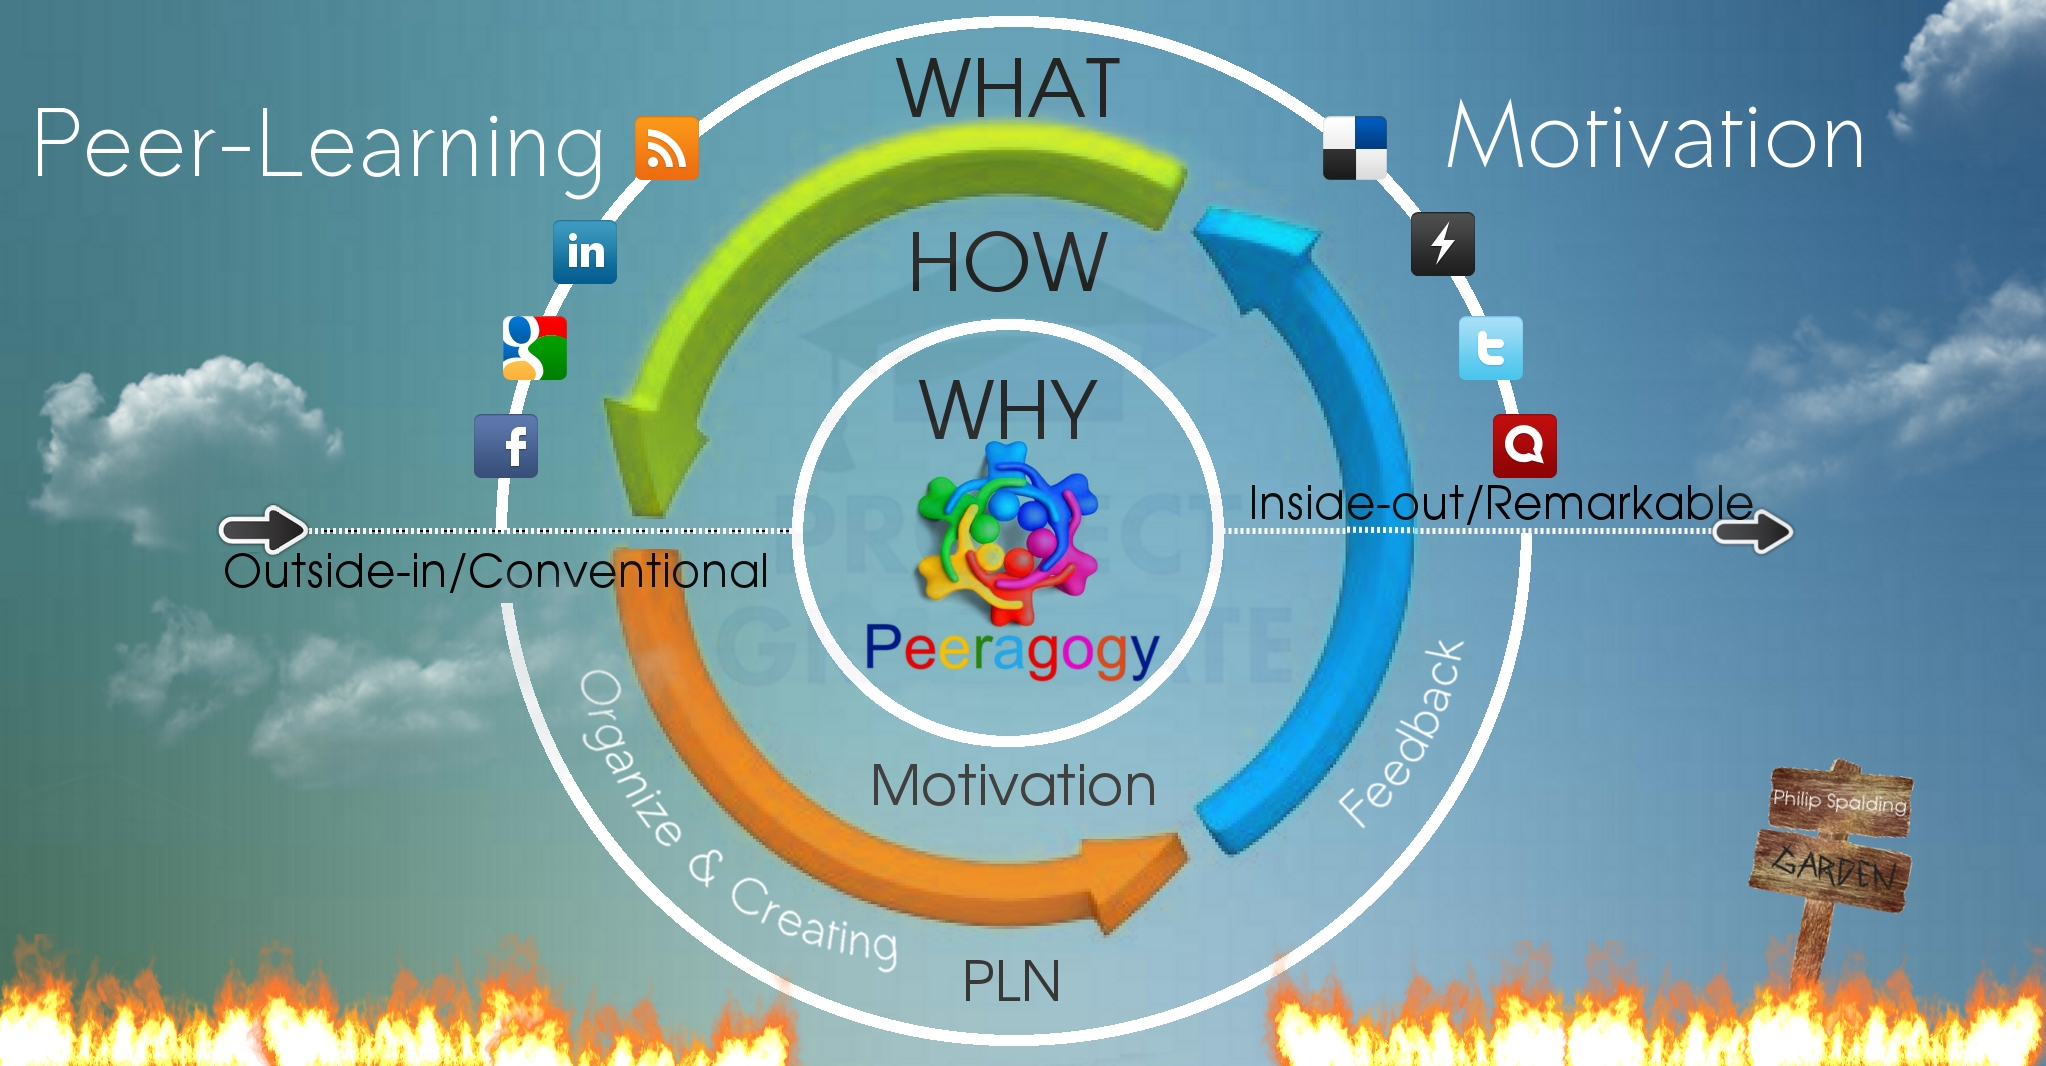
\includegraphics{http://peeragogy.org/wp-content/uploads/2013/01/44272.jpg}

%% \emph{``What's my motivation?''}

\section*{Example: Peeragogy editor Charlotte Pierce}

Basically, I'm here because as an early adopter and admitted gadget
freak, I find it fun and rewarding to explore new technologies and
topics that I feel have a practical or exciting application. But I have
some some other motivations that subtly co-exist alongside my eagerness
to explore and learn.

Howard Rheingold's reputation as an innovator and internet pioneer got
my attention when he announced his Think-Know Tools course on Facebook
in 2012. I had known of Howard from the 1990's when I was a member of
The WELL (Whole Earth `Lectronic Link). I was curious to see what Howard
was up to, so I signed onto the wiki site, paid my \$300, and took the
course starting in October.

Looking back, I realize we were practicing Peeragogy throughout the TKT
course, though at the time I hardly knew peer learning from a pickle. In
late November, missing the camaraderie and challenge of TKT, I stepped
over to check out the \emph{Peeragogy Handbook}.

Which brings me to motivations in signing on to Peeragogy. Since Howard
and several Think-Know Tools co-learners were already dedicating their
time here and their work looked innovative and exciting, I suspected
they might be onto something that I wanted to be a part of. Plus, my
brain was primed by the TKT experience. ``What if a diverse group of
people could learn a subject with little or no cost and not a lot of
barriers to entry,'' I thought. ``What if their own experience qualified
them to join, contribute, and learn.''

I also thought there might be a chance to meet some potential business
partners or clients there - but if not, the experience looked rewarding
and fun enough for me to take the risk of no direct remuneration. There
was no up front cost to me, and a wealth of knowledge to gain as a part
of something new and exciting. These are always big draws for me. I
wanted to be in on it, and nobody was telling me I couldn't!

My projections proved correct. The participants already on board were
gracious in welcoming me to Peeragogy, patient in getting me up to
speed, and persistent in coaxing me into using the tools central to the
project. I connected, learned, grew, and contributed. Now I'm on the
brink of starting a peer learning project of my own in my publishing
organization, IPNE.org. Stay tuned!

\section*{Example: Cafes, schools, workshops}

Suppose we wanted to make Peeragogy into a model that can be used in
schools, libraries, and so forth, worldwide - and, in fact we do! ~How
can we bring the basic Peeragogy motivations to bear, and make a
resource, plan of action, and process that other people can connect
with? ~In brief, how do we build peer learning into the
curriculum, providing new insight from the safety of the existing
structure?

One concrete way to implement these broad aims would be to make a
peeragogy-oriented \emph{development} project whose goal is to set up a
system of internet cafes, schools, or workshops in places like China or
Africa, where people could go to collaborate on work or to learn
technical subjects. Students could learn on the job. It seems reasonable
to think that investors could make a reasonable profit through
``franchises,'' hardware sales, and so forth -- and obviously making
money is a motivation that most people can relate to.

In developing such a project, we would want to learn from other similar
projects that already exist. ~For example, in Chicago, State Farm
Insurance has created a space called the
``\href{https://www.nextdoorchi.com/}{Next Door Cafe}'' that runs
community events. One of their offerings is free financial coaching,
with the explicit agreement that the issues you discuss return to State
Farm as market research.

\begin{quote}
\textbf{State Farm Insurance}: ``Free? Really. Yes, because we're
experimenting.  We want to learn what people really want. Then, we'll
shoot those wants back to the Farm. We help you. You help us
innovate. We're all smarter for it. We think it's a win-win.''
\end{quote}

Thus, Next Door Cafe forms part of a system to exploit the side-effects
of interpersonal interactions to create a system that learns.~ A peer
learning example from the opposite side of the world started in a slum
next to New Delhi where Sugata Mitra gave children a computer and they
self organized into a learning community and taught themselves how to
use the machine and much more.

\begin{quote}
\textbf{Sugata Mitra}: ``I think what we need to look at is we need to
look at learning as the product of educational self-organization. If
you allow the educational process to self-organize, then learning
emerges.  It's not about making learning happen. It's about letting it
happen.''
\end{quote}

In 2014, we tried a similar experiment.  We asked: Can we build a
``\href{http://commonsabundance.net/docs/help-build-the-peeragogy-accelerator-work-in-progress/}{Peeragogy
  Accelerator}'' for a half-dozen peer learning projects, each of
which defines their own metrics for success, but who come together to
offer support and guidance, using the \emph{Peeragogy Handbook} as a
resource?  We tried that with several our own projects, and benefitted
from the peer support.  Several months later, we found the Accelerator
format even more exciting when we ran a one-off series focusing on
Sagarika Bhatta's research on adaptation to climate change in Nepal.
Our sense is that peeragogy could be useful for building a global
support network around just about any project.  Peeragogy can support
a culture of real engagement, rather than ``clicktivism,'' and the
direct exchange of critically-assessed effort rather than
often-inefficient donations of cash [3].

\subsubsection{References}

\begin{enumerate}
\itemsep1pt\parskip0pt\parsep0pt
\item
  Hugo Mercier and Dan Sperber (2011). Why do humans reason? Arguments
  for an argumentative theory, \emph{Behavioral and Brain Sciences}, 34,
  57-111.
\item
  Jérôme~Hergueux (2013). \href{https://cyber.law.harvard.edu/interactive/events/luncheons/2013/11/jerome}{Cooperation
  in a Peer Production Economy: Experimental Evidence from Wikipedia},
  talk presented at the Berkman Center for Internet and Society.
\item  Kevin Edmonds (2012).
Beyond Good Intentions: The Structural Limitations of NGOs in Haiti.  \emph{Critical Sociology}, 39(3).
\end{enumerate}

%
\chapter[\textbf{Case Study: 5PH1NX}]{Case Study: 5PH1NX}\label{sphinx-beginning}
%
\begin{quote}
5PH1NX: 5tudent Peer Heuristic for 1Nformation Xchange - we think of it
as a ``curiously trans-media'' use case in peeragogical assessment.
\end{quote}
\emph{Author:} David Preston

\begin{quote}
Over the last several decades technology has driven massive shifts in
the way we communicate and collaborate. Information technology,
socioeconomic trends, an increasingly complex and uncertain future, and
school's failed brand are contributing factors in an emerging discourse
that seeks to align learning with our rapidly changing culture.

Open Source Learning and Peeragogy, two emerging theoretical frameworks
in this discourse, leverage end-to-end user principles of communication
technology to facilitate peers learning together and teaching each
other. In both traditional and liminal learning communities, one of the
major points of contact between education and societal culture is the
purposeful use of assessment. The processes of giving, receiving, and
applying constructive critique makes learners better thinkers,
innovators, motivators, collaborators, coworkers, friends, relatives,
spouses, teammates, and neighbors. Implementing peer-based assessment
can be problematic in schooling institutions where evaluative authority
is traditionally conflated with hierarchical authority, and where
economic and political influences have focused attention on summative,
quantitative, standardized measurement of learning and intelligence.

This is the story of how one learning community is adopting Open Source
Learning and Peeragogical principles to decentralize and enrich the
assessment process.

\textbf{Aldous Huxley}: Knowledge is acquired when we succeed in fitting
a new experience into the system of concepts based upon our old
experiences. Understanding comes when we liberate ourselves from the old
and so make possible a direct, unmediated contact with the new, the
mystery, moment by moment, of our existence.

\end{quote}
\subsection{Enter 5PH1NX}

On Monday, April 2, 2011, students in three English classes at a
California public high school discovered anomalies in the day's entry on
their course blog. (Reminder: not so long ago this sentence would have
been rightly interpreted as being science fiction.) The date was wrong
and the journal topic was this:

\begin{quote}
In The Principles of Psychology (1890), William James wrote, "The
faculty of voluntarily bringing back a wandering attention, over and
over again, is the very root of judgment, character and will. No one is
\emph{compos sui} if he have it not. An education which should improve
this faculty would be the education par excellence." How have your
experiences in this course helped you focus your attention? What do you
still need to work on? What elements of the following text (from Haruki
Murakami's \emph{1Q84}) draw your attention and help you construct
meaning? The driver nodded and took the money. ``Would you like a
receipt?'' ``No need. And keep the change.'' ``Thanks very much,'' he
said. ``Be care\textbf{f}ul, it looks windy out there. Don't
sl\textbf{i}p.'' ``I'll be careful,'' Aomame said. ``A\textbf{n}d
also,'' the \textbf{d}river said, facing \textbf{t}he mirror, ``please
remember: t\textbf{h}ings are not what they seem.'' Things are not what
they seem, Aomame repeated mentally. ``What do you mean by that?'' she
asked with knitt\textbf{e}d brows. The driver chose his words carefully:
``It's \textbf{j}ust that y\textbf{o}u're about to do something out of
the ordinary. Am I right? People do not ordinarily climb down the
emergency stairs of the Metropolitan Expressway in the middle of the
day-- especially women.'' ``I suppose you're right.'' ``Right. And after
you do something like that, the everyday loo\textbf{k} of things might
seem to chang\textbf{e} a little. Things may look
\emph{diffe\textbf{r}ent} to you than they did before. I've had that
experience myself. But don't let appearance\textbf{s} fool you. There's
always only one reality.''
\end{quote}
\subsection{Find the jokers}

\begin{figure}
\centering
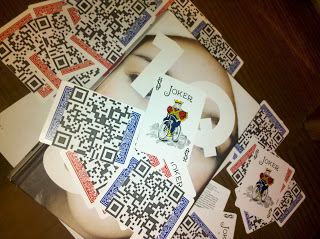
\includegraphics[width=.8\textwidth]{../pictures/jokers.jpg}
\end{figure}

The jokers were real {[}4{]} and hidden (without much intent to conceal)
around the classroom and in students' journals. Students found them and
asked questions about the letters in bold; the questions went
unanswered. Some thought it was just another of their teacher's wild
hair ideas. Although they didn't know it yet they were playing the
liminal role that Oedipus originated in mythology. Solving the riddle
would enable them to usher out an old way of thinking and introduce the
new. The old way: An authority figure sets the rules, packages the
information for a passive audience, and unilaterally evaluates each
learner's performance. In that context, peeragogical assessment might be
introduced with a theoretical framework, a rubric, and a lesson plan
with input, checks for understanding, and guided practice as a
foundation for independent work. The new way: In Open Source Learning
the learner pursues a path of inquiry within communities that function
as end-to-end user networks. Each individual begins her learning with a
question and pursues answers through an interdisciplinary course of
study that emphasizes multiple modalities and the five Fs: mental
Fitness, physical Fitness, spiritual Fitness, civic Fitness, and
technological Fitness. Learners collaborate with mentors and receive
feedback from experts, community-based peers, and the public. They are
the heroes of learning journeys. Heroes don't respond to syllabi. They
respond to calls to adventure. Open Source Learning prepares students
for the unforeseen. By the time they met the 5PH1NX students had learned
about habits of mind, operating schema, digital culture and community,
self-expression, collaboration, free play, autonomy,
confidence/trust/risk, and resilience. These ideas had been reinforced
through nonfiction articles and literary selections such as Montaigne's
Essays, Plato's Allegory of the Cave, Bukowski's Laughing Heart,
Shakespeare's Hamlet, Sartre's No Exit and others. The first poem
assigned in the course was Bukowski's
``\href{http://www.youtube.com/watch?v=bHOHi5ueo0A}{Laughing Heart}?'':
\emph{The Gods will offer you chances. Know them. Take them.} So it is
with knowledge and understanding. Today we are presented with an
overwhelming, unprecedented quantity and variety of data in our physical
and virtual lives; to cope we must improve the ways we seek, select,
curate, analyze, evaluate, and act on information. On the back of each
Joker card was a QR code that linked to a blog page with riddles and
clues to a search. At this point students realized they were playing a
game. A tab on the blog page labeled ``The Law'' laid out the rules of
engagement:

\subsection{This is The Law}

\begin{enumerate}[itemsep=0pt]
\item
  You cannot ``obey'' or ``break'' The Law. You can only make good
  decisions or bad decisions.
\item
  Good decisions lead to positive outcomes.
\item
  Bad decisions lead to suffering.
\item
  Success requires humanity.
\item
  ``For the strength of the Pack is the Wolf, and the strength of the
  Wolf is the Pack.'' -Rudyard Kipling
\item
  ``The Way of the sage is to act but not to compete.'' -Lao Tzu
\item
  Be honorable.
\item
  Have fun.
\item
  Question.
\item
  \emph{Sapere aude}.
\end{enumerate}
This is The Law. After a second set of on-campus and blog quests,
students noticed a shift in 5PH1NX. A couple of weeks before the first
clue was published, during a Socratic seminar on Derrida's concept of
Free Play, a student said, ``We learn best when adults take away the
crutches and there is no safety net.''? The quote was used in the next
clue; students began to realize that the game was not pre-determined.
5PH1NX was evolving in response to their contributions. This is a
manifestation of the hackneyed writing cliché: show, don't tell. The
student's comment was a call to action. The Feats of Wisdom were
designed to engage learners over a vacation break in fun, collaborative,
social media-friendly missions that required engagement in the
community, expansion of their personal learning networks, and
documentation on their blogs. For example:

\subsubsection{FEAT \#1}

\emph{Buy a ticket to ``The Hunger Games'' (or any other movie that's
likely to draw a large, young, rowdy audience). Before the lights dim
and the trailers begin, walk to the screen, turn to the audience, and in
a loud, clear voice, recite the ``To be, or not to be\ldots{}''
soliloquy from Hamlet (don't worry if you make a couple mistakes, just
be sure you make it all the way to, ``Be all my sins remembered.'').
\href{http://alarhsenglitcomp.blogspot.com/2012/12/feats-of-wisdom-1\_15.html}{Capture
the event on video \& post it to your blog.}} Students had been using
the Internet without an Acceptable Use Policy all year; such policies
are one-to-many artifacts of a central authority and far weaker than
community norms. So rather than introduce ``rules'' 5PH1NX simply
provided a reminder of the client-side responsibility.

\subsection{The Emergence of Peeragogical Assessment}

The third page on the Feats of Wisdom blog was entitled
\emph{Identifying and Rewarding Greatness}, where learners were greeted
with the following paragraph:

\begin{quote}
If you see something that was done with love, that pushed the
boundaries, set the standard, broke the mold, pushed the envelope,
raised the bar, blew the doors off, or rocked in some previously
unspecified way, please bring it to the attention of the tribe by
posting a link to it {[}here{]}.
\end{quote}
No one did. Instead, they started doing something more effective. They
started building. One student hacked the entire game and then created
her own version. Other students began to consider the implications for
identifying and rewarding greatness. They realized that one teacher
couldn't possibly observe how 96 students were working over vacation out
in the community and online to accomplish the Feats of Wisdom. In order
to get credit for their efforts they would have to curate and share
their work-process and product. They also realized that the same logic
applied to learning and coursework in general; after all, even the most
engaged, conscientious teacher only sees a high school or college
student a few hours a week, under relatively artificial conditions. The
learner presumably spends her whole life in the company of her own
brain. Who is the more qualified reporting authority? With these
thoughts in mind students created \emph{Project Infinity}, a
peer-to-peer assessment platform through which students could
independently assign value to the thoughts and activities they deemed
worthy. Because the 2011-12 5PH1NX was a three-week exercise in
gamification, \emph{Project Infinity} quickly evolved to include
collaborative working groups and coursework. This was learner-centered
Peeragogical assessment in action; learners identified a need and an
opportunity, they built a tool for the purpose, they managed it
themselves, and they leveraged it in a meaningful way to support student
achievement in the core curriculum.

\subsection{Project Infinity 2 \& Implications for the Future}

Alumni from the Class of 2012 felt such a strong positive connection to
their experience in Open Source Learning and Peeragogical assessment
that they built a version for the Class of 2013. They created
\emph{Project Infinity2} with enhanced functionality. They asked the
teacher to embed an associated Twitter feed on the course blog, then
came to classes to speak with current students about their experiences.
Everyone thought the Class of 2013 would stand on the shoulders of
giants and adopt the platform with similar enthusiasm. They were wrong.
Students understood the concept and politely contributed suggestions for
credit, but it quickly became evident that they weren't enthusiastic.
Submissions decreased and finally the \emph{Project Infinity2} Twitter
feed disappeared from the course blog. Learners' blogs and project work
suggested that they were mastering the core curriculum and meta
concepts, and they appeared generally excited about Open Source Learning
overall. So why weren't they more excited about the idea of assessing
themselves and each other? Because \emph{Project Infinity2} wasn't
theirs. They didn't get to build it. It was handed to them in the same
way that a syllabus is handed to them. No matter how innovative or
effective it might be, \emph{Project Infinity2} was just another tool
designed by someone else to get students to do something they weren't
sure they wanted or needed to do in the first place. Timing may also be
a factor. Last year's students didn't meet 5PH1NX until the first week
in April, well into the spring semester. This year's cohort started
everything faster and met 5PH1NX in November. In January they understood
the true potential of their situation started to take the reins. As
students realized what was happening with the clues and QR codes they
approached the teacher and last year's alumni with a request: ``Let Us
In.'' They don't just want to design learning materials or creatively
demonstrate mastery, they want to chart their own course and build the
vehicles for taking the trip. Alumni and students are becoming Virtual
TAs who will start the formal peer-to-peer advising and grading process.
In the Spring Semester all students will be asked to prepare a statement
of goals and intentions, and they will be informed that the traditional
teacher will be responsible for no more than 30\% of their grade. The
rest will come from a community of peers, experts and members of the
public. On Tuesday of Finals Week, 5PH1NX went from five players to two
hundred. Sophomores and freshman have jumped into the fray and
hacked/solved one of the blog clues before seniors did. Members of the
Open Source Learning cohort have also identified opportunities to enrich
and expand 5PH1NX. A series of conversations about in-person retreats
and the alumni community led to students wanting to create a massively
multiple player learning cohort. Imagine 50,000-100,000 learners
collaborating and sharing information on a quest to pass an exam by
solving a puzzle that leads them to a ``Learning Man Festival''? in the
Summer of 2013. When 5PH1NX players return from Winter Break in January
they will transform their roles relative to the game and the course.
Several have already shared ``AHA!'' moments in which they discovered
ways to share ideas and encourage collaboration and peer assessment.
They have identified Virtual Teaching Assistant candidates, who will be
coached by alumni, and they have plans to provide peer-based assessment
for their online work. They are also now actively engaged in taking more
control over the collaboration process itself. On the last day of the
semester, a post-finals throwaway day of 30-minute class sessions that
administrators put on the calendar to collect Average Daily Attendance
money, hardly anyone came to campus. But Open Source Learning students
were all there. They have separated the experience of learning from the
temporal, spatial, and cultural constraints of school. They understand
how democracy works: those who participate make the decisions. No one
knows how this ends, but the outcome of Peeragogical assessment is not a
score; it is learners who demonstrate their thinking progress and
mastery through social production and peer-based critique. This
community's approach to learning and assessment has prepared its members
for a complex and uncertain future by moving them from a world of
probability to a world of possibility. As one student put it in a video
entitled ``We Are Superman,'' ``What we are doing now may seem small,
but we are part of something so much bigger than we think. What does
this prove? It proves everything; it proves that it's possible.''

\subsection{Background}

A world in which work looks more like what's described in the PSFK
\textbf{\href{http://www.slideshare.net/PSFK/psfk-presents-future-of-work-report}{Future
of Work Report 2013}} requires a new learning environment.

The problem is that tools and strategies such as MOOCs, videos, virtual
environments, and games are only as good as the contexts in which they
are used. Even the most adept practitioners quickly discover that
pressing emerging technology and culture into the shape of yesterday's
curricular and instructional models amounts to little more than
Skinner's Box 2.0. So what is to be done? How can we use emerging tools
and culture to deliver such an amazing individual and collaborative
experience that it shatters expectations and helps students forget
they're in school long enough to fall in love with learning again?

Education in the Information Age should enable learners to find,
analyze, evaluate, curate, and act on the best available information.
Pursuing an interdisciplinary path of inquiry in an interest-based
community doesn't just facilitate the acquisition of factual knowledge
(which has a limited half-life). The process brings learners closer to
understanding their own habits of mind and gives them practice and an
identity in the culture they'll be expected to join after they graduate.
This requires new literacies and a curriculum that emphasizes mental
fitness, physical fitness, spiritual fitness, civic fitness, and
technological fitness.

Models of assessment that emphasize self-directed and collaborative
Peeragogical principles enrich the learning experience and accelerate
and amplify deep understanding. Because these approaches are pull-based
and generate tens of thousands of multi- or trans-media data points per
learner, they also generate multi-dimensional portraits of learner
development and provide feedback that goes far beyond strengths and
weaknesses in content retention. The long-term benefit is exponential.
Learners who can intentionally direct their own concentration are
empowered far beyond knowledge acquisition or skill mastery. They become
more effective thinkers and -- because they are invested -- more caring
people. This learning experience is of their own making: it isn't
business, it's personal. The inspiration to recreate the process for
themselves and for others is the wellspring of the lifelong learner.

As Benjamin Disraeli put it, ``In general the most successful man in
life is the man who has the best information.'' It is a widely accepted
truism in business that better data leads to better decisions. We now
have the ability to generate, aggregate, analyze, and evaluate much
richer data sets that can help us learn more about helping each other
learn. Sharing richer data in different ways will have the same game
changing effect in learning that it has in professional sports and
investment banking.

Self-directed, collaborative assessment generates an unprecedented
quantity and variety of data that illuminates aspects of learning,
instruction, and overall systemic efficacy. Even a quick look at readily
available freeware metrics, blog/social media content, and time stamps
can provide valuable insight into an individual's working process and
differentiate learners in a network.

In the larger scheme of things, Peeragogical assessment provides direct
access to and practice in the culture learners will be expected to join
when they complete their course of study. Collaboration, delegation,
facilitating conversations, and other highly valued skills are developed
in plain view, where progress can be critiqued and validated by peers,
experts and the public.

But tall trees don't grow by themselves in the desert. Peeragogical
innovation can be challenging in organizational cultures that prioritize
control and standardization; as Senge \emph{et al}. have observed, the
system doesn't evaluate quality when dealing with the unfamiliar, it
just pushes back. In schools this is so typical that it doesn't merit
comment in traditional media. The world notices when Syria goes dark,
but in school, restricted online access is business as usual.

Cultural constraints can make early adopters in technology-based
Peeragogy seem like Promethean risk-takers. Whenever the author gives a
talk or an interview, someone asks if he's in trouble.

Learners are not fooled by the rhetoric of in loco parentis or vision
statements that emphasize ``safe, nurturing learning environments.''
With notable exceptions, today's school leaders do not know as much
about technology as the young people for whom they assume
responsibility. Still, learners understand survival: they are fighting
in unfavorable terrain against an enemy of great power. Innovating is
impossible, and even loudly criticizing school or advocating for change
is a risk. As a result many do just enough to satisfy requirements
without getting involved enough to attract attention. Some have also
internalized the critical voices of authority or the failure of the
formal experience as evidence of their own inability: ``I'm just not
good at math.''

How do we know when we're really good at something? Standardized testing
feedback doesn't help learners improve. Most of us don't have a natural
talent for offering or accepting criticism. And yet, as Wole Soyinka put
it, ``The greatest threat to freedom is the absence of criticism.''?
Peeragogical interaction requires refining relational and topical
critique, as well as skills in other ``meta'' literacies, including but
not limited to critical thinking, collaboration, conflict resolution,
decision-making, mindfulness, patience and compassion.

Interpersonal learning skills are undervalued in today's schooling
paradigm. Consequently there is an operational lack of incentive for
teachers and learners to devote time and energy, particularly when it
carries a perceived cost in achievement on tests that determine
financial allocations and job security. In recent years there has been
increasing pressure to tie teacher compensation, performance evaluation,
and job status directly to student performance on standardized tests.

Some educators are introducing peer-to-peer network language and even
introducing peer-based assessment. But the contracts, syllabi and
letters to students typically stink of \emph{the old way}. These
one-to-many documents are presented by agents of the institution endowed
with the power to reward or punish. To many students this does not
represent a choice or a real opportunity to hack the learning
experience. They suspect manipulation, and they wait for the other shoe
to drop. Learners also don't like to be told they're free while being
forced to operate within tight constraints. Consider this likely
reaction to a policy that is highly regarded in the field:

\begin{quote}
``Students may choose to reblog their work in a public place or on their
own blogs, but do so at their own risk.'' \emph{What? Did I read that
correctly?} ``Students may choose to reblog their work in a public place
or on their own blogs, but do so at their own risk.''\emph{Risk? What
risk? The risk of possibly helping someone understand something that
they didn't before, or get a different opinion than the one they had
before? Someone please help me make sense of this.}

\end{quote}
To effectively adopt Peeragogical assessment in the schooling context,
the community must construct a new understanding of how the members in a
network relate to one another independent of their roles in the
surrounding social or hierarchical systems. This requires trust, which
in school requires significant suspension of disbelief, which -- and
this is the hard part -- requires actual substantive, structural change
in the learning transaction. This is the defining characteristic of Open
Source Learning: as the network grows, changes composition, and changes
purpose, it also changes the direction and content of the learning
experience. Every network member can introduce new ideas, ask questions,
and contribute resources than refine and redirect the process.

This isn't easy. A member in this network must forget what she knows
about school in order to test the boundaries of learning that shape her
relationship to content, peers, and expert sources of information and
feedback. This is how the cogs in the machine become the liminal heroes
who redesign it. Having rejected the old way, they must now create the
rituals that will come to define the new. They are following in the path
of Oedipus, who took on the inscrutable and intimidating Sphinx, solved
the riddle that had killed others who tried, and ushered out the old
belief systems to pave the way for the Gods of Olympus. Imagine, what
if Oedipus had the Internet.



\part{Peeragogy in Practice} \label{practice-part}  %%%%%%%%%%%%%%%%%%%%
%
\chapter[\textbf{Thinking about patterns}]{Thinking about patterns}
\begin{quote}
Although a grounding in learning theory helps inform peer learning
projects, Peeragogy, at its core, comes to life in applied practice.
Even before convening a group for your peer learning project, you will
want to take a look over the patterns we have collected here. You will
likely return here many times as your project develops.

\end{quote}
\subsection{What is a pattern?}

A pattern is anything that has a repeated effect. In the context of
peeragogy, the practice is to repeat processes and interactions that
advance the learning mission. Frequent occurrences that are not
desirable are called anti-patterns!

\begin{quote}
\textbf{Christopher Alexander}: ``Each pattern describes a problems
which occurs over and over again in our environment, and then describes
the core of the solution to that problem, in a way that you can use this
solution a million times over, without ever doing it the same way
twice.'' {[}1{]}

\end{quote}
Patterns provide a framework that can be applied to similar issues but
may be metaphorically solved in different ways, sometimes in real world
or face to face events and other times in digital space. Outside of
Alexander's own work in architecture, one the first groups to adopt a
design pattern way of thinking about things were computer programmers.
Writing in the foreward to Richard P. Gabriel's \emph{Patterns of
Software}, Alexander emphasizes that the key question to ask about any
design approach is: does it help us build better?

\begin{quote}
\textbf{Christopher Alexander}: ``What is the Chartres of programming?
What task is at a high enough level to inspire people writing programs,
to reach for the stars?'' {[}2{]}

\end{quote}
We think that Peeragogy stands a good chance of being a ``killer app''
for pattern-based design. Learning bridges physical and virtual worlds
all the time. And, in fact, a \emph{Network of Learning} was the 18th
pattern that Christopher Alexander introduced in his book, \emph{A
Pattern Language}.

\begin{quote}
\textbf{Christopher Alexander}: ``Work in piecemeal ways to decentralize
the process of learning and enrich it through contact with many places
and people all over the city: workshops, teachers at home or walking
through the city, professionals willing to take on the young as helpers,
older children teaching younger children, museums, youth groups
travelling, scholarly seminars, industrial workshops, old people, and so
on.'' {[}1{]}

\end{quote}
Peeragogy can help to extend and enrich this network, and, as we shall
see, patterns can be used by those involved to do ongoing ``emergent''
design, not only by building new structures, but by adapting and
improving our catalog of patterns as we go.

\subsection{Patterns of peeragogy}

Here is our index of the main patterns we've found so far (described in
more detail after the jump):

\begin{itemize}
\item
  \textbf{\href{http://peeragogy.org/patterns/wrapper/}{Wrapper}} - Front end
  appearance to participants. Consolidate and summarize.
\item
  \textbf{\href{http://peeragogy.org/patterns/discerning-a-pattern/}{Discerning
  a pattern}} - Found a pattern? Give it a title and record an example.
  (Woah, meta!)
\item
  \textbf{\href{http://peeragogy.org/patterns/polling-for-ideas/}{Polling for
  ideas}} - Invite brainstorming, collecting ideas, questions, and
  solutions.
\item
  \textbf{\href{http://peeragogy.org/patterns/creating-a-guide/}{Creating a
  guide}} - Overviews expose the lay of the land. Collecting content and
  stories.
\item
  \textbf{\href{http://peeragogy.org/patterns/newcomer/}{Newcomer}} - Create a
  guide for ``beginner's mind'' and help avoid need to introduce new
  members each ``meeting.''
\item
  \textbf{\href{http://peeragogy.org/patterns/roadmap/}{Roadmap}} - Plans for
  future work, direction towards a goal, dynamic
\item
  \textbf{\href{http://peeragogy.org/patterns/roles/}{Roles}} - Specialize and
  mix it up. Play to participants strengths and skills.
\item
  \textbf{\href{http://peeragogy.org/focusing-on-a-specific-project/}{Project
  focus}} - Lightbulb moment: Most specific projects involve learning!
\item
  \textbf{\href{http://peeragogy.org/patterns/carrying-capacity/}{Carrying
  capacity}} - Know your limits, find ways to get other people involved.
\item
  \textbf{\href{http://peeragogy.org/patterns/heartbeat/}{Heartbeat}} - The
  ``heartbeat'' of the group keeps energy flowing.
\item
  \textbf{\href{http://peeragogy.org/patterns/moderation/}{Moderation}} - When
  leaders step back, dynamics can improve; moderator serves as champion
  and editor.
\item
  \textbf{\href{http://peeragogy.org/patterns/praxis-vs-poeisis/}{Use or make?}}
  - Repurposing, tinkering, or creating from scratch?
%% \item
%%   \textbf{\href{http://peeragogy.org/reiterate/}{Reiterate} - Periodically
%%   review and revise actions as needed
\end{itemize}
We'll introduce three additional patterns in the chapter on
\href{http://peeragogy.org/to-peeragogy/researching-peeragogy/}{researching
peeragogy}.

\subsection{Anti-patterns for Peeragogy}

And some ``anti-patterns'' (things to avoid if possible):

\begin{itemize}
\item
  \textbf{\href{http://peeragogy.org/antipatterns/isolation/}{Isolation}} - A
  tale of silos, holes, and not-invented-here.
\item
  \textbf{\href{http://peeragogy.org/antipatterns/magical-thinking/}{Magical
  thinking}} - ``One meeting will (not) change everything!''
\item
  \textbf{\href{http://peeragogy.org/antipatterns/co-learning-messy-with-lurkers/}{Messy
  with Lurkers}} - What happens when joining is low-cost and completion
  is low-benefit.
\item
  \textbf{\href{http://peeragogy.org/antipatterns/misunderstanding-power/}{Misunderstanding
  Power}} - The workload is almost never evenly distributed.
\item
  \textbf{\href{http://peeragogy.org/antipatterns/navel-gazing/}{Navel Gazing}} -
  ``I have this really great idea\ldots{}''
\item
  \textbf{\href{http://peeragogy.org/antipatterns/stasis/}{Stasis}} - What is the
  driver behind open source, commons-oriented collaborative projects?
  (Because, let's face it, it doesn't always work.)
\item
  \textbf{\href{http://peeragogy.org/antipatterns/stuck-at-the-level-of-weak-ties/}{Stuck
  at the level of weak ties}} - Can we deepen the connection?
\end{itemize}
\subsection{What is a use case?}

A use case describes someone (or something) who uses a given system or
tool to achieve a goal. A use case can include a title, a summary of the
problem, an actor, and a success scenario. Additional features can be
added, such as alternate interactions or choices that lead to a
variation on the result.

The use case considers a given persona (a characteristic role) in a
given situation and shows how they works on a project/problem and how
their process of work is resolved into a solution or solutions. Some
activities do not have a single solution -- these are often referred to
as ``Wicked Problems.'' With detailed bookkeeping effort, recorded
processes can be standardized into use cases that can then be employed
directly or modified to fit the context of the activity at hand. In
short, they are a lot like design patterns, which they may contain in
hidden or explicit form. Use cases are presented in vignettes that
appear throughout the book (like the one at the end of this section).

\subsection{A peeragogy pattern language}

By looking at how patterns combine in real and hypothetical use cases,
you can start to identify a \emph{pattern language} that can be used in
your projects. We can get a simplified view of these connections with
the following diagram. It's important to clarify that everyone doesn't
do it the same way. Here, the \emph{Roadmap} is given a central
position, but some peer learning projects will forego making a specific,
detailed plan; their plan is just to see what develops. You can see here
how peeragogy patterns often break down further into individual
micro-steps: we'll say more about that shortly.

\begin{figure}[htbp]
\centering
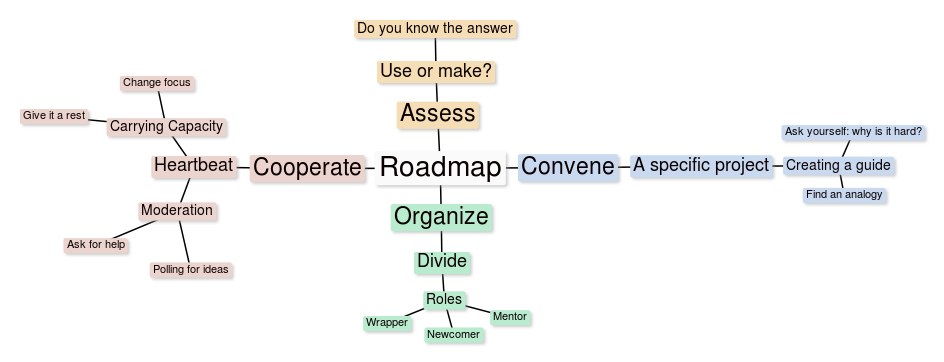
\includegraphics[width=\textwidth]{../pictures/pattern-language.jpg}
%\caption*{A map of some of the main features of our pattern language}
\end{figure}

The subsequent main sections of this book --
\href{http://peeragogy.org/convene/}{\emph{Convene}},
\href{http://peeragogy.org/organize/}{\emph{Organize}},
\href{http://peeragogy.org/facilitate/}{\emph{Cooperate}} and
\href{http://peeragogy.org/assessment/}{\emph{Assess}} -- represent big
clusters of patterns that are likely to come up time and again in
various projects. We can think of these as East, South, West, and North
in the diagram above. You are of course encouraged to invent your own
patterns and to connect them in new ways. Each project has a unique
design, and it's own unique way in which things play out in practice.
What we've put together here is a starter kit.

\begin{quote}
\textbf{Christopher Alexander}: These ideas---patterns---are hardly more
than glimpses of a much deeper level of structure, and is ultimately
within this deeper level of structure, that the origin of life occurs.
{[}2{]}
\end{quote}
\subsection{Patterns and Problem Solving}

Ten potentially useful things to do when you're solving a problem are
described by the computer scientist Marvin Minsky in a series of
\href{http://web.media.mit.edu/~minsky/OLPC-1.html}{m}\href{http://web.media.mit.edu/~minsky/OLPC-2.html}{e}\href{http://web.media.mit.edu/~minsky/OLPC-3.html}{m}\href{http://web.media.mit.edu/~minsky/OLPC-4.html}{o}\href{http://web.media.mit.edu/~minsky/OLPC-5.html}{s}
written for the One Laptop Per Child project. We can sum them up
visually with the following diagram:

\begin{figure}[htbp]
\centering
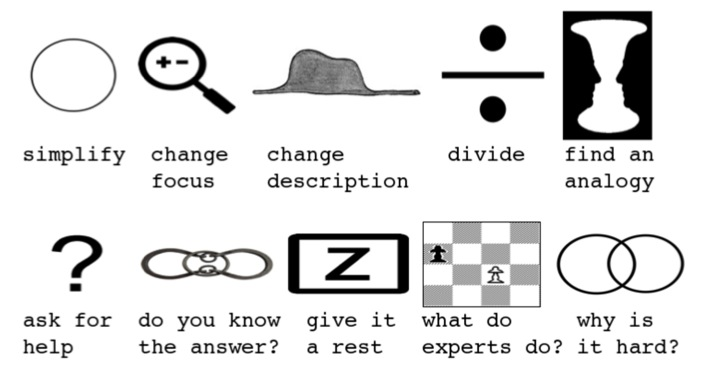
\includegraphics[width=\textwidth]{../pictures/heuristic-images.jpg}
\caption*{}
\end{figure}

We can also see some interesting connections between these intuitive
problem solving heuristics and peeragogy patterns listed above. This can
help illustrate further connections between the patterns, and some of
the ways that groups can apply them to solve real-world problem. To
elaborate briefly:

\begin{itemize}
\item
  Simplify things for \textbf{Newcomers}. We don't expect a newcomer to
  enter at full speed.
\item
  Use a \textbf{Roadmap} to guide us from one phase to another, while
  the project's central \textbf{Heartbeat} helps us attend to the
  central focus.
\item
  Announce changes through a \textbf{Wrapper} who describes the new
  status or direction of the project. For the Peeragogy project, that
  often meant summing up the high points that we saw over a given period
  of time.
\item
  We divide work up not only horizontally among different
  \textbf{Roles}, but also temporally by using the \textbf{Roadmap}.
  Someone who is moving ahead with the Roadmap is likely to be working
  at the leading edge.
\item
  When we find an analogy, we are basically \textbf{Creating a Guide}
  for thinking about something. This can be used as a form of
  ``exploration,'' as we look at how one form of engagement may or may
  not map onto other forms of engagement.
\item
  When we ask for help, we may avail ourselves of some
  \textbf{Moderation} service that will decide how to deal with our
  request. One simple way to ask for help is \textbf{Polling for Ideas}.
  Obviously once we start to get help, we're working in a regime of
  ``collaborative effort''.
\item
  If you know the answer, then you may be able to reuse it (which is the
  basic idea described in \textbf{Use or Make}.
\item
  It is important to give it a rest so as not to over-exhaust oneself,
  busting one's own \textbf{Carrying Capacity}, or, alternatively,
  overwhelming the group.
\item
  It seems that one of the things that experts are good at is
  \textbf{Discerning a Pattern}. This allows them to simplify their
  processing.
\item
  Finally, again, if we know why it is hard, then we may be able to
  \textbf{Create a Guide} that will help get around, or at least better
  cope with, the difficulty.
\end{itemize}

\subsubsection{References}

\begin{enumerate}
\item
  Alexander, Christopher, Ishikawa, Sara, and Silverstein, Murray,
  \emph{A Pattern Language: Towns, Buildings, and, Construction}, New
  York: Oxford University Press, 1977.
\item
  Gabriel, Richard P.
  \emph{\href{http://dreamsongs.net/Files/PatternsOfSoftware.pdf}{Patterns
  of Software}}, New York: Oxford University Press, 1996. (Includes a
  forward by Christopher Alexander.)
\end{enumerate}

%
\chapter[\textbf{Patterns}]{ Patterns }

\section*{Wrapper}
\paragraph{The Definition:} The wrapper role can be taken on by a project
participant who summarizes everything going on in the project, making
the project comprehensible to participants who haven't been following
all of the details.

\paragraph{The Problem:} Joining the project that is already going can feel
like trying to get aboard a rapidly moving vehicle. If you've joined and
then taken time off, you may feel like things have moved on so far that
it's impossible to catch up. In a very active project, it can be
effectively impossible to stay up to date with all of the details.

\paragraph{The Solution:} Charlie
Danoff \href{http://socialmediaclassroom.com/host/peeragogy/wiki/rolesdivision-labor}{suggested}
that someone take on the ``wrapper role'' -- do a weekly pre/post wrap,
so that new (and existing) users would know the status the project is at
any given point in time. The
project's \href{http://socialmediaclassroom.com/host/peeragogy/}{landing
page} also serves as another sort of ``wrapper'', telling people what
they can expect to find.

\paragraph{Objectives:} In fulfilling the wrapper role, we must check the
public summaries of the project from time to time to make sure that they
accurately represent the facts on the ground.

\paragraph{Examples:} In the first year of the Peeragogy project, the
``Weekly Roundup'' by Christopher Tillman Neal served to engage and
re-engage members. Peeragogues began to eager watched for the weekly
reports to see if our teams or our names had been mentioned. When there
was a holiday or break, Chris would announce the hiatus, to keep the
flow going. In the second year of the project, we didn't routinely
publish summaries of progress, and instead, we've assumed that
interested parties will stay tuned on Google+. Nevertheless, we maintain
internal and external summaries, ranging from agendas to press releases
to quick-start guides. Regular meetings provide an alternative way to
stay up to date: see
the \href{http://peeragogy.org/patterns/heartbeat/}{Heartbeat} pattern.

\paragraph{Challenges:} According to the theory proposed by Yochai Benkler,
for free/open ``commons-based'' projects to work, it is vital to have
both (1) the ability to contribute small pieces; (2) something that
stitches those pieces together {[}1{]}. The wrapper performs this
integrative function, which is often much more challenging than the job
of breaking things down into pieces or just doing one of the small
pieces.

\paragraph{What's Next:}
We need better practices for wrapping things up at
various levels.  One of the latest ideas is to develop a simple visual
``dashboard'' for the project.

\paragraph{Reference:}

\begin{enumerate}
\itemsep1pt\parskip0pt\parsep0pt
\item
  Benkler, Y.
  (2002). \href{http://www.yale.edu/yalelj/112/BenklerWEB.pdf}{Coase's
  Penguin, or Linux and the Nature of the Firm}, Yale Law Journal 112,
  pp. 369-446.
\end{enumerate}

\section*{Discerning a Pattern}
Discerning patterns helps us build our vocabulary or repertoire for
peer-learning projects. As a very simple example, in building a peer
learning profile, a participant might identify an interest such as
organic gardening. We begin to notice that this is a pattern when it
repeats -- when organic gardening is frequently listed among the
interests listed by participants in their self-introductions. The
classic example of an architectural pattern is "\emph{A place to wait}"
\emph{---}a type of space found in many architectural and urban design
projects. Once a pattern is detected, give it a title and write down how
the pattern works. For example, what does this pattern say about the
self-selection process of the group? Without jumping to conclusions,
consider that an interest in organic gardening, for example, might
indicate the participants are oriented to cooperation, personal health,
or environmental activism. How does the pattern relate to other patterns
already listed in this catalog?

\section*{Polling for Ideas}
\ldots{} and then Howard said \emph{``At the beginning,
until we all know the ropes well enough to understand when to create a
new discussion forum topic and when to add to an existing one, let's
talk in this topic thread about what else we want to discuss and I
will start new topic threads when necessary.''}

Polling for Ideas can happen at many junctures in a peer learning
experience, e.g. we could poll for ideas about ``who would we like to
join our group?'', and ``what would be good resources for us to use?''

\section*{Creating a Guide}
Meaning-carrying tools, like handbooks or maps, can help people use an
idea. In particular, when the idea or system is only ``newly
discovered'', the associated meanings may not be well understood (indeed
they may not have been created). In such a case, the process of creating
the guide can go hand-in-hand with figuring out how the system works.
Thus, techniques of \href{http://knowledgecartography.org/}{knowledge
cartography} and
\href{http://www.hitl.washington.edu/publications/r-97-47/two.html}{meaning
making} are useful for would-be guide creators. Even so, it is worth
noting that ``the map is not the territory,'' and map-making is only one
facet of shared human activity. Collaboratively refining a pattern is
itself an example of ``Creating a Guide'' - that is, a pattern
description can be thought of as a ``micro-map'' of a specific activity.

\section*{Newcomer}
Unless there is a new person to talk to, a lot of the ``education
stuff'' we do could get kind of stale. Many of the patterns and use
cases for peeragogy assume that there will be an audience or a new
generation of learners - hence things like creating a \emph{guide}. Note
that the \emph{newcomer} and the \emph{wrapper} may work together to
make the project accessible.

Even in the absence of actual newcomers, we're often asked to try and
look at things with a ``beginner's mind.'' Note: Regis has written
\href{http://socialmediaclassroom.com/host/peeragogy/forum/suggest-new-discussion-topics\#comment-1796}{practical
advice} for things we can do on behalf of newcomers in this project.

\section*{Roadmap}
It is very useful to have an up-to-date public roadmap for the project,
someplace where it can be discussed and maintained.~ This
helps~\textbf{newcomers} know where they can jump in.~ It also gives a
sense of the accomplishments to date, and any major challenges that lie
ahead.~ Remember, the Roadmap exists as an artifact with which to share
current, but never complete, understanding of the space.~ Never stop
learning!

\subsubsection{Examples}

\textbf{}In the Peeragogy project, now that the outline is fairly
mature, we can use it as a roadmap, by marking the sections that are
``finished'' (at least in draft), marking the sections where editing is
currently taking place, and marking the stubs (possible starting points
for future contributors).~ While this does not provide a complete
roadmap for all aspects of the project, it does give editors a sense of
what is going on.~ The Free Technology Guild provides one
\href{http://campus.ftacademy.org/wiki/index.php/Free\_Technology\_Guild\_Roadmap}{example}.

\subsubsection{And also}

Note that a shared roadmap is very similar to a
\href{http://peeragogy.org/to-peeragogy/personal-learning-plan/}{Personal
Learning Plan}, or ``paragogical profile''.~ We've made some
\href{http://campus.ftacademy.org/wiki/index.php/Free\_Technology\_Guild\#Learning\_design}{examples}
of these as we got started working on the Free Technology Guild. ~

\section*{Roles}
\paragraph{Definition:} Educational interactions tend to have a number of
different roles associated with them. Everything could bifurcate from
the ``autodidact'', as in, (1) Autodidact, (2) Tutor-Tutee, (3)
Tutor-Tutee-Peer, etc., until we have bursars, librarians, technicians,
janitors, editors of peer reviewed research journals, government policy
makers, spin-off industrial ventures and partnerships, and so on.

\paragraph{Problem:} Even the autodidact may assume different roles at
different points in time - sometimes building a library, sometimes
constructing a model, sometimes checking a proof. The decomposition of
``learning'' into different phases or polarities could be an endless
theoretical task. The simpler problem is to be aware of the roles that
you and your teammates have in the projects you're working on.

\paragraph{Solution:} We've described some exercises on
``\href{http://peeragogy.org/can-we-work-together/}{metacognition}''
that you can apply when thinking about the roles that you're taking on
and those that you'd like to take on in your project.

\paragraph{Challenges:} Roles are often present ``by default'' at the start
of a learning process, and that they may change as the process develops.
Both of these features can be challenging, but they also present
learning opportunities.

\paragraph{What's Next:} We've listed some of the roles for which we're
seeking volunteers in
the\href{http://peeragogy.org/peeragogy-org-roadmap/}{Peeragogy.org
Roadmap}: Volunteer Coordinator, Seminar Coordinator, Usability Guru,
Activities Master, and Tech lead. As with everything else in the
roadmap, this list should be reviewed and revised regularly, as the
roles are understood relative to the actual happenings in the Peeragogy
project.

\section*{Focusing on a specific project}
In the Jan. 2013 plenary session, as \href{http://IPNE.org}{Independent
Publishers of New England} (IPNE) President Tordis Isselhardt quietly
listened to a presentation about how we created the \emph{Peeragogy
Handbook}. During the Q\&A, he spoke up, wondering if peer-learning
effort in IPNE might be more likely to succeed if the organization's
members ``focused around a specific project.'' As this lightbulb
illuminated the room, those of us attending the plenary session
suggested that IPNE could focus the project by creating an ``Independent
Publishing Handbook.'' (Applause!) 

In the course of creating the IPNE Handbook, peer learners would
assemble resource repositories, exchange expertise, and
collaboratively edit documents. To provide motivation and incentive to
participate in ``PeerPubU'', members of the association will earn
authorship credit for contributing articles, editor credit for working
on the manuscript, and can spin off their own chapters as stand-alone,
profit-making publications.

\section*{Carrying Capacity}
\begin{quote}
\emph{``If overstimulation at the sensory level increases the distortion
with which we perceive reality, cognitive overstimulation interferes
with our ability to `think.'\,'' --}\emph{Future Shock}, by Alvin
Toffler
\end{quote}

\begin{center}
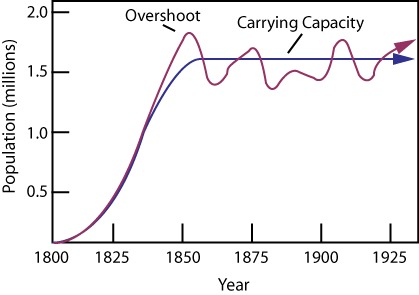
\includegraphics[width=.65\textwidth]{../pictures/carrying_capacity.jpg} \\
Image from
\href{http://missbakersbiologyclasswiki.wikispaces.com/Ecology+Study+Guide}{Miss
Baker's Biology Class Wiki} (CC-By-NC-SA).
\end{center}

At times, a facilitator or participant in the peer-learning enterprise
may feel he or she is over-contributing -- or, perhaps more likely, that
others are under-contributing -- or that someone else is railroading an
idea or dominating the discussion. If this happens, take a step back and
observe the dynamics of involvement. Ask questions and let others
answer. Especially if you start to feel the symptoms of burnout, it's
important that you find the level of engagement that allows you to
participate at a level that is feasible for maintaining progress toward
the project's goal. Lead by example -- but make sure it's someplace you,
and others, actually want to go! This could be a good time to revisit
the group's roadmap and see if you can figure out and clarify to others
what concrete goal you're working towards. Remember that you can also
change the ``landscape'' by making it easier for other people to get
involved -- for example, by explaining what you're trying to do in a
clear manner. Watch for opportunities to step back, watch, listen. Try
to be mindful of phases when active or quiet involvement would be more
helpful to the individual and the group. It's also helpful to let anyone
who has taken on a facilitation role know if you're stepping back
temporarily. Then, when the time is right, step back in and get to work!

\section*{Heartbeat}
\paragraph{Definition:} The project's heartbeat is a recurring activity,
something that makes it so that people experience a ``there, there.''

\paragraph{Problem:} Without someone or something acting as the heartbeat
for the group, energy may dissipate.

\paragraph{Solution:} People seem to gravitate to regularly scheduled
activities. Sometimes people need a little extra prompt to join in.

\paragraph{Examples:} In the ``Collaborative Lesson Planning'' course led
by Charlie Danoff at P2PU, Charlie wrote individual emails to people who
were signed up for the course and who had disappeared, or lurked but
didn't participate. This kept a healthy number of the people in the
group to re-engage and make positive contributions. In more recent
months, Charlotte Pierce has been running weekly meetings by Google
Hangout to coordinate work on the Peeragogy Handbook. Not only have we
gotten a lot of hands-on editorial work done this way, we've generated a
tremendous amount of new material (both text and video footage) that is
likely to find its way into future versions of the book.

\paragraph{Challenges:} Meetings that happen for the sake of having a
meeting are almost a bad joke. Be aware of the energy that's there
before and after meetings. If the energy isn't sustaining you or your
group, think about what needs to change.

\paragraph{What's Next:} When the project is bigger than more than just a
few people, it's likely you'll get several heartbeats -- for instance,
we've recently been running two weekly meetings in the Peeragogy
project, for members with slightly different interests and slightly
different availability. Finding ways to communicate across these
different ``camps'' is useful.

\section*{Moderation}
\paragraph{Definition:} Moderation seems to have a double meaning: there's
moderation as in moderation in all things and moderation as in keeping a
discussion going smoothly. Actually, both of them are about the same
thing.

\paragraph{Problem:}
\href{http://peeragogy.org/organizing-a-learning-context/participation/}{Participation}
in online forums tends to follow a ``power law,'' with vastly unequal
engagement.

\paragraph{Solution:} If you want to counteract this tendency, one
possibility would simply be for the most active participants to step
back, and moderate how much they speak. This is related the the
\href{http://peeragogy.org/patterns-usecases/patterns-and-heuristics/carrying-capacity/}{Carrying
Capacity} pattern and the
\href{http://peeragogy.org/practice/antipatterns/misunderstanding-power/}{Misunderstanding
Power} anti-pattern: check those out before you proceed.

\paragraph{Examples:} Occupy Wall Street used a technique that they called
the ``\href{http://en.wikipedia.org/wiki/Progressive_stack}{progressive
stack}.'' There are lots of other strategies to try.

\begin{quote}
\textbf{The Co-Intelligence Institute}: Why is a fishbowl more
productive than debate? The small group conversations in the fishbowl
tend to de-personalize the issue and reduce the stress level, making
people's statements more cogent. Since people are talking with their
fellow partisans, they get less caught up in wasteful adversarial games.
\end{quote}

\paragraph{Challenges:} In a distributed project, there are many
side-conversations, and it is impossible (and would be undesirable) for
any one person to moderate all of them. The difficulty occurs if one of
these conversations becomes uncomfortable for one or more participants,
for whatever reason. Rather than depending on one central moderator,
it's useful for everyone in the project to be aware of the principles
underlying effective moderation, and apply them together even in small
side-projects.

\paragraph{What's Next:} We recently ran a Paragogical Action Review to
elicit feedback from participants in the Peeragogy project. Some of them
brought up dissatisfactions, and some of them brought up confusion. Can
we find ways to bring these concerns front-and-center, without
embarrassing the people who brought them up?

%\section*{Pattern Language}
%I use the idea of a \emph{pattern language} as a shorthand for what
Christopher Alexander talks about in his
\href{http://www.patternlanguage.com/archive/ieee/ieeetext.htm}{keynote
address} for the IEEE in 1996.

In short, once we have come up with enough patterns (including the
pattern of a \emph{pattern language} that I discussing here, and its
generalizations per Christopher Alexander), then we will be better able
to do both the socio-technical design work associated with planning
pæragogical experiences, and, quite likely, enjoy the ``actual work''
more too.

In this quote from the linked article, C. A. talks about computer
programming, but I think the same could go for any other sort of
design-and-implementation work:

\begin{quote}
\emph{It is a view of programming as the natural genetic infrastructure
of a living world which you/we are capable of creating, managing, making
available, and which could then have the result that a living structure
in our towns, houses, work places, cities, becomes an attainable thing.
That would be remarkable. It would turn the world around, and make
living structure the norm once again, throughout society, and make the
world worth living in again.This is an extraordinary vision of the
future, in which computers play a fundamental role in making the world -
and above all the built structure of the world - alive, humane,
ecologically profound, and with a deep living structure.}
\end{quote}

\section*{Use or Make?}
\begin{quote}
``Praxis, a noble activity, is always one of use, as distinct from
poesis which designates fabrication. Only the former, which plays and
acts, but does not produce, is noble.'' {[}1{]} (p. 101)
\end{quote}

There is a tension between ``making stuff'' and ``using stuff''. Peer
\emph{production}, as the name indicates, is about ``making stuff,''
or~\href{http://en.wikipedia.org/wiki/Poiesis}{poesis}. And stuff is, at
least in theory, kinda cool.~ Furthermore, some of the most familiar
examples of peeragogy in practice come from the craft and maker
movements.~ However, we can also try to be aware of just how much
``learning'' is really ``remix'' -- re-use and recycling of other
people's ideas and techniques.~ Understanding and negotiating the
tension between reuse and creativity is key to the art of remix.

\subsubsection{Reference}

\begin{enumerate}
\item
  Baudrillard, J. (1975). \emph{The mirror of production}. Telos Press
\end{enumerate}



\chapter[\textbf{Antipatterns}]{Antipatterns}

\section*{Isolation}
\paragraph{Definition:} Many projects that are ostensibly oriented towards
``the commons'' nevertheless want to funnel participants into ``their
way'' of thinking about things. Be careful with that, it's a slippery
slope to total isolation.

\paragraph{Problem:} This problem is actually dual: with a too-narrow
focus, collaboration is impossible. However, with an overly-wide focus,
things are chaotic in other ways.

\paragraph{Solution:}

\begin{quote}
\textbf{Félix Guattari}: Imagine a fenced field in which there are
horses wearing adjustable blinkers, and let's say that the ``coefficient
of transversality'' will be precisely the adjustment of the blinkers. If
the horses are completely blind, a certain kind of traumatic encounter
will be produced. As soon as the blinkers are opened, one can imagine
that the horses will move about in a more harmonious way.
(\href{http://nine.fibreculturejournal.org/}{Quoted by Andrew Murphy},
himself quoting Gary Genosko)
\end{quote}

%\includegraphics{http://upload.wikimedia.org/wikipedia/commons/d/dd/Muybridge_race_horse_animated.gif}

Like the underlying problem, the solution is has two sides to it: you can avoid
isolation by becoming highly transversal -- or avoid noise and chaos by
blinkering yourself and shutting out other things.  

\paragraph{Challenges:} The challenge, of course, is that it's hard not to over-correct.  The moderate interpretation of the quote is
that it's good to be open, but not too open.  We need to allow for
uncertainty, but not be completely vague.  Not so easy. (See
also: \href{http://peeragogy.org/antipatterns/navel-gazing/}{Navel
Gazing}.)

\paragraph{What's Next:} We recently submitted an abstract called ``Escape
from Peeragogy Island'' to a geography conference talking about the
spatiality of peer production. The idea behind this article is that we
feel like we've come up with something great with the Peeragogy project,
but we're going to be a bit isolated if it's not transparently useful to
others. If we can't explain why it's a great idea, then it's not
entirely clear how great of an idea it actually is.

\section*{Magical thinking}
\paragraph{Definition:} While we could imagine an ideal information
processing system that would (magically) come with all solutions
pre-built, a more realistic approach recognizes that real problem
solving always takes time and energy.

\paragraph{Problem:} Given a difficult problem, we usually want to take a
shortcut.

\paragraph{Solution:} Magical thinking robs a context of its ``process'' or
``motion''. The more completely we fall back on ``traditional'' modes of
doing things (including magical ones) the less we stand to learn. It's
also true that traditions and habits can serve a useful function: they
can massively simplify and streamline, and adopting some healthy habits
can free up time and energy, making learning possible. But if we try
something new and imagine that things work the way they always have
(e.g. sign up for a course and get told what to do, then do it and
pass), we can run into trouble when the situation doesn't match our
preconceptions.

\paragraph{Example:} Joe Corneli's 2011 DIY Math course at P2PU went quite
badly. Students signed up hoping to learn mathematics, but none of them
had very concrete goals about what to learn, or very developed knowledge
about how to study this subject. This was what the class was supposed to
help teach. However, it seemed as if the students felt that signing up
for the course would ``magically'' give them the structure they needed.
Still, it's not as if the blame can be placed entirely on the students
in this case. Building a learning space with no particular structure and
saying, ``go forth and self-organize!''~is not likely to work, either.
The one saving grace of DIY Math is that the course post-mortem informed
the development of the paragogy principles: it was not a mistake we
would repeat again.

\paragraph{Challenges:} If we already ``knew'', 100\%, how to do peeragogy,
then we would not stand to learn very much by writing this handbook.
Difficulties and tensions would be resolved ``in advance''. We know
this, but readers may still expect ``easy answers''.

\paragraph{What's Next:} Fast-forwarding a few years from the DIY Math
experiment: as part of the PlanetMath project, we are hoping to build a
well-thought-through example of a peer learning space for mathematics.
One of the ideas we're exploring is to use patterns and antipatterns
(exactly like the ones in this catalog) as a way not only of designing a
learning space, but also of talking about the difficulties that people
frequently run into when studying mathematics. Building an initial
collection of Calculus Patterns may help give people the guide-posts
they need to start effectively self-organizing.



\section*{Messy with Lurkers}
\begin{quote}
\textbf{Gigi Johnson}\emph{: (1) Co-learning is Messy. It needs time,
patience, confusion, re-forming, re-norming, re-storming, etc. Things go
awry and part of norms needs to be how to realign. (2) Co-learning is a
VERY different experience from traditional teacher-led learning in terms
of time and completion. It is frustrating, so many people will lurk or
just step in and out, the latter of which is very different from what is
acceptable in traditonal learning. Online learning programs are painted
with the brush now of an ``unacceptable'' 50\% average non-completion
rate. Stanford's MOOC AI class, which started out with +100,000 people,
had 12\% finish. If only 12\% or 50\% of my traditional class finished,
I'd have a hard time getting next quarter's classes approved!}
\end{quote}
The second point is similar to the earlier Anti-pattern
``\href{http://socialmediaclassroom.com/host/peeragogy/forum/anti-patterns-concerns-complaints-and-critiques\#comment-1854}{Misunderstanding
Power (Laws)}``. People have to join in order to try, and when joining
is low-cost, and completion low-benefit, it is not surprising that many
people will''dissipate" as the course progresses. The ``messiness'' of
co-learning is interesting because it points to a sort of ``internal
dissipation'', as contributors bring their multiple different
backgrounds, interests, and communication styles to bear. In
\href{http://www.altchi.org/submissions/submission\_wmt\_0.pdf}{Tomlinson
et al.}, we observed:

\begin{quote}
\emph{More authors means more content, but also more words thrown away.
Many of the words written by authors were deleted during the ongoing
editing process. The sheer mass of deleted words might raise the
question of whether authoring a paper in such a massively distributed
fashion is efficient.}
\end{quote}
If we were to describe this situation in traditional subject/object
terms, we would say that peer production has a ``low signal to noise
ratio''. However, it may be more appropriate (and constructive) to think
of meanings as co-constructed as the process runs, and of messiness (or
meaninglessness) as symptomatic, not of peer production \emph{itself},
but of deficiencies or infelicities in shared meaning-making and
``integrating'' features.

\section*{Misunderstanding Power}
\begin{quote}
\textbf{Wikipedia}: Zipf's law states that given some corpus of natural
language utterances, the frequency of any word is inversely proportional
to its rank in the frequency table. Thus the most frequent word will
occur approximately twice as often as the second most frequent word,
three times as often as the third most frequent word, etc. {[}1{]}
\end{quote}
Zipf's law (or other formulations of the same thing) govern the
\href{http://www2.econ.uu.nl/users/marrewijk/geography/zipf/index.htm}{size
of cities}, and related formulations describe
\href{http://pricetags.wordpress.com/2010/10/26/kleibers-law-growth-and-creativity-in-cities/}{energy
use}: roughly speaking, an elephant has a lower metabolism than a mouse
and is more ``energy efficient''. At that same link, we see the
suggestion that creativity and other social network effects speed up as
population grows! \emph{The anti-pattern}: how many times have we been
at a conference or workshop and heard someone say (or said ourselves)
``wouldn't it be great if this energy could be sustained all year
'round?'' Or in a classroom or peer production setting, wondered why it
is that everyone does not participate equally. ``Wouldn't it be great if
we could increase participation?'' But participation in a given
population is going falls off according to \emph{some} power law (see
Introduction to Power Laws in
\href{http://www.theuncertaintyprinciple.danoff.org/v2i3.html}{The
Uncertainty Principle, Volume II, Issue 3}). It would be a grand
illusion to assume that everyone is coming from a similar place with
regard to the various literacies and motivations that are conducive to
participation. Furthermore, a ``provisionist'' attitude (``If we change
our system we will equalize participation and access'') simply will not
work in general. Power laws are an inherent epiphenomenon of network
flow. Certainly, if you can
\href{http://peeragogy.org/practice/moderation/}{moderate} the way the
network is shaped, you can change the ``exponent'' -- for example, by
helping more people develop relevant literacies. But even so,
``equality'' remains a largely abstract notional. Note, as well, that
participation in a given activity tends to fall off over time. Many
people would like to write a hit song or a best selling novel or start a
religion, etc., but few actually do, because it takes sustained effort
over time. See the anti-pattern
``\href{http://peeragogy.org/antipatterns/magical-thinking/}{Magical
Thinking}'' for more on this. Our ability to develop new literacies is
limited. Much as Paul Graham wrote about programming languages --
programmers are typically ``satisfied with whatever language they happen
to use, because it dictates the way they think about programs'' -- so
too are people often ``satisfied'' with their social environments,
because these tend to dictate the way they think and act in life.

\subsubsection{Reference}

\begin{enumerate}
\item
  \href{http://en.wikipedia.org/w/index.php?title=Zipf\%27s\_law\&oldid=575709945}{Zipf's
  law}. (2013). In \emph{Wikipedia, The Free Encyclopedia}.
\item
  Graham, P. (2001). \href{http://www.paulgraham.com/avg.html}{Beating
  the averages}.
\end{enumerate}

\section*{Navel Gazing}
\paragraph{Definition:} The difficulty breaks down like this:

\begin{enumerate}
\item
  Certainly we cannot get things done just by talking about them.
\item
  And yet, feedback can be useful, i.e., if there are mechanisms for
  responding to it in a useful fashion.
\item
  The associated anti-pattern is a special case of the prototypical
  Batesonian \href{http://en.wikipedia.org/wiki/Double_bind}{double
  bind}, ``the father who says to his son: go ahead, criticize me, but
  strongly hints that all effective criticism will be very unwelcome''
  {[}1{]}, p. 88.
\end{enumerate}

\paragraph{Problem:} Criticism is not always useful. Sometimes it is just
``noise''.

\paragraph{(Bogus) Solution:} It's tempting to create ``open'' systems that
inadvertantly replicate the double bind -- by being open to criticism,
but unable to act on it effectively.

\paragraph{Challenges:} A long list of criticisms that haven't been dealt
with is maybe better than no communication at all, but it's also a
tell-tale sign of deeper dissatisfaction. It's better to make sure you
have enough bandwidth (see
\href{http://peeragogy.org/patterns-usecases/patterns-and-heuristics/carrying-capacity/}{Carrying
Capacity}) for dealing with a given class of problems and issues. Adjust
your focus accordingly, but be careful (see
``\href{http://peeragogy.org/antipatterns/isolation/}{Isolation}'').

\paragraph{What's Next:} We have hinted that, in this project,
\href{http://peeragogy.org/how-to-use-this-handbook/}{effective
criticism is very welcome}! But understanding what makes criticism
effective is, in general, still a research problem.

\paragraph{Reference:}

\begin{enumerate}
\itemsep1pt\parskip0pt\parsep0pt
\item
  Deleuze, G., and Guattari, F. (2004). \emph{Anti-oedipus}. Continuum
  International Publishing Group.
\end{enumerate}

\section*{Stasis}
Actually, living beings are never \emph{really} in stasis. It just
sometimes feels that way. Different anti-patterns like
\href{http://socialmediaclassroom.com/host/peeragogy/forum/anti-patterns-concerns-complaints-and-critiques\#comment-2267}{Isolation}
or
\href{http://socialmediaclassroom.com/host/peeragogy/forum/anti-patterns-concerns-complaints-and-critiques\#comment-1808}{Navel-Gazing}
have described different aspects of the \emph{experience} of feeling
like one is in stasis. Typically, what is happening in such a case is
that one or more dimensions of life are moving very slowly.

For instance, we were not able to get programming support to improve the
first version of the Social Media Classroom, for love or money, since
all developer energy was going into the next version. This isn't true
stasis, but it can feel frustrating when a specific small feature is
desired, but unavailable.

The solution? Don't get hung up on small things, and find the dimensions
where movement \emph{is} possible. In a sense this is analogous to
eating a balanced diet. You probably shouldn't only eat grilled cheese
sandwiches, even if you like them a lot. You should go for something
different once in a while.

This is also related to the pattern that talks about
``\href{http://socialmediaclassroom.com/host/peeragogy/forum/patterns-and-use-cases\#comment-2320}{Carrying
Capacity}''. There is always some dimension on which you can make
progress -- it just might not be the same dimension you've recently
over-harvested!

\section*{Stuck at the level of weak ties}
Remember this from our article on
\href{http://peeragogy.org/organizing-a-learning-context/}{organizing a
learning context}?

\begin{quote}
\emph{There is a certain irony here: we are studying ``peeragogy'', and
yet many respondents did not feel they were really getting to know one
another ``as peers''. Several remarked that they learned less from other
individual participants, and more from ``the collective''. Those who did
have a ``team'', or who knew one another from previous experiences, felt
more peer-like in those relationships.}
\end{quote}
\subsubsection{Are weak ties ``strong''?}

``Weak ties'' are often deemed a strength: see for example
\href{http://www.psychologytoday.com/blog/thinking-about-kids/201005/facebook-and-the-strength-weak-ties}{this
article} in Psychology Today, which says:

\begin{quote}
"\emph{{[}S{]}trong and weak ties tend to serve different functions in
our lives. When we need a big favor or social or instrumental support,
we ask our friends. We call them when we need to move a washing machine.
But if we need information that we don't have, the people to ask are our
weak ties. They have more diverse knowledge and more diverse ties than
our close friends do. We ask them when we want to know who to hire to
install our washing machine.}"
\end{quote}
The quote suggests that there is a certain trade-off between use of weak
ties and use of strong ties. The anti-pattern in question then is less
to do with whether we are forming weak ties or strong ties, and more to
do with whether we are being \emph{honest with ourselves and with each
other about the nature of the ties we are forming} -- and their
potential uses. We can be ``peers'' in either a weak or a strong sense.
The question to ask is whether our needs match our expectations!

In the peeragogy context, this has to do with how we interact. One of
the participants in this project wrote:

\begin{quote}
"\emph{I am learning about peeragogy, but I think I'm failing {[}to
be{]} a good peeragog{[}ue{]}. I remember that Howard {[}once{]} told us
that the most important thing is that you should be responsible not only
for your own learning but for your peers' learning. {[}\ldots{}{]} So
the question is, are we learning from others by ourselves or are we
{[}\ldots{}{]} helping others to learn?}"
\end{quote}
If we are ``only'' co-consumers of information (which happens to
``produced'' live, by some of the participants), then this seems like a
classic example of a weak tie. We are part of the same ``audience'' --
or anyway, in the same ``theater'' (even if separated from each other by
continuous ``4th walls''). On the other hand, actively engaging with
other people (whether with ``my'' learning, with ``their'' learning, or
with the co-production of knowledge) seems to be the foundation for
strong ties. In this case our aims (or needs) are more instrumental, and
less informational.

People who do not put in the time and effort will remain stuck at the
level of ``weak ties'', and will not be able to draw on the benefits
that ``strong ties'' offer.


\chapter[\textbf{A pattern story}]{A pattern story}
%
\emph{October, 2011}. Tom's day-job involves finding patterns in market
data (see
\href{http://www.ted.com/talks/kevin_slavin_how_algorithms_shape_our_world.html}{Kevin
Slavin's TED talk}). He reads philosophy and does some other programming
work in his spare time. However, he doesn't take the Occupy Wall Street
protest very seriously. But one of these evenings, one of the protestors
catches his attention. She's dressed rather strikingly. They talk, and
he comes away thinking about something she said:
``\emph{\href{http://www.nycga.net/files/2011/11/DeclarationFlowchart_v2_large.jpg}{All
our grievances are interconnected}.}'' What if all the solutions are
interconnected too? Night time: Tom becomes increasingly obsessed with
this idea. He's pulling down lots of web pages from the internet ---
again, looking for patterns. What would it take for OWS folks to solve
the problems they worry so much about? He starts working on a tool
that's geared towards learning and sharing skills, while working on real
projects. At first, it's just hackers who are using the tool, but over
time they adapt it for popular use. Things start to get
interesting\ldots{} {[}caption id=``'' align=``aligncenter''
width=``465''{]}\href{http://peeragogy.org/a-pattern-story/matrix/}{
\includegraphics{http://peeragogy.org/wp-content/uploads/2013/12/matrix.jpg}}
Multiple PSK31 transmissions on the 20m digital modes band at around
14.07 MHz.
\href{https://commons.wikimedia.org/wiki/File:PSK_matrix.jpg}{Public
Domain image} by User:Mysid{[}/caption{]}



\part{Convening A Group} \label{convening-part} %%%%%%%%%%%%%%%%%%%%
%
\chapter[\textbf{Convening}]{Building Your Co-Learning Group}
\begin{quote}
So you've decided to try peer learning? Maybe you've already found a few
people who will support you in this effort. Congratulations! It's time
now to focus your thinking. How will you convene others to form a
suitable group? How will you design a learner experience which will make
your project thrive? In this chapter, we suggest a variety of questions
that will help you to make your project more concrete for potential new
members. There are no good or bad answers - it depends on the nature of
your project and the context. Trying to answer the questions is not
something you do just once. At various stages of the project, even after
it's over, some or all of those questions will aquire new meanings - and
probably new answers.
\end{quote}

\begin{quote}
\textbf{Fabrizio Terzi}: ``There is a force of attraction that allows
aggregation into groups based on the degree of personal interest; the
ability to enhance and improve the share of each participant; the
expectation of success and potential benefit.''
\end{quote}

\subsection{Group identity}\label{group-identity}

Note that there are many groups that may not need to be ``convened'',
since they already exist. There is a good story from
\href{http://www.sarvodayausa.org/learn/a-t-ariyartne/}{A. T.
Ariyaratne} in his
\href{http://www.sarvodaya.org/about/philosophy/collected-works-vol-1/rural-self-help}{collected
works} in which he does ``convene'' a natural group (a village) - but in
any case, keep in mind at the outset that the degree of
group-consciousness that is necessary for peer learning to take place is
not fixed. In this section, we suppose you are just at the point of
kicking off a project. What steps should you take? We suggest you take a
moment to ponder the following questions first - and revisit them
afterward, as a way to identify best practices for the next effort.

\subsection{There will be a quiz}\label{there-will-be-a-quiz}

Those taking the initiative should ask themselves the traditional Who,
What, Where, When, Why, and How.
(\href{http://en.wikipedia.org/wiki/Simon_Sinek}{Simon Sinek} suggests
to begin with Why, and we touched on Who, above!). In doing so,
preliminary assumptions for design and structure are established.
However, in peer learning it is particularly important to maintain a
healthy degree of openness, so that future group members can also form
their answers on those questions. In particular, this suggests that the
design and structure of the project (and the group) may change over
time. Here, we riff on the traditional 5W's+H with six clusters of
questions to~help you focus your thinking about the project and amplify
its positive outcomes.

\subsection{Expectations for
participants}\label{expectations-for-participants}

\textbf{1. Who: Roles and flux}

\begin{itemize}
\itemsep1pt\parskip0pt\parsep0pt
\item
  What are some of the roles that people are likely to fall into
  (e.g.~Newcomer, Wrapper, Lurker, Aggregator, etc.)?
\item
  How likely is it that participants will stick with the project? If you
  expect many participants to leave, how will this effect the group and
  the outcome?
\item
  Do you envision new people joining the group as time goes by? If so,
  what features are you designing that will support their integration
  into an existing flow?
\item
  Will the project work if people dip in and out? If so, what features
  support that? If not, how will people stay focused?
\end{itemize}

\textbf{2. What: Nature of the project}

\begin{itemize}
\itemsep1pt\parskip0pt\parsep0pt
\item
  What skills are required? What skills are you trying to build?
\item
  What kinds of change will participants undergo? Will they be heading
  into new ground? Changing their minds about something? Learning about
  learning?
\item
  What social objective, or ``product'' if any, is the project aiming to
  achieve?
\item
  What's the `hook?'~Unless you are working with an existing group, or
  re-using an existing modality, consistent participation may not be a
  given.
\end{itemize}

\textbf{3. When: Time management}

\begin{itemize}
\itemsep1pt\parskip0pt\parsep0pt
\item
  What do you expect the group to do, from the moment it convenes, to
  the end of its life-span, to create the specific outcome that will
  exist at the conclusion of its last meeting? {[}2{]} Note that what
  people ACTUALLY do may be different from what you envision at the
  outset, so you may want to revisit this question (and your answer)
  again as the project progresses.
\item
  Keeping in mind that at least one period of is inertia is very likely
  {[}2{]}, what event(s) do you anticipate happening in the group that
  will bring things back together, set a new direction, or generally get
  things on track? More generally, what kinds of contingencies does your
  group face? How does it interface to the ``outside world''?
\item
  What pre-existing narratives or workflows could you copy in your
  group?
\item
  How much of a time commitment do you expect from participants? Is this
  kind of commitment realistic for members of your group?
\item
  What, if anything, can you do to make participation ``easy'' in the
  sense that it happens in the natural flow of life for group members?
\item
  Does everyone need to participate equally? How might non-equal
  participation play out for participants down the line?
\end{itemize}

\textbf{4. Where: Journey vs Destination}

\begin{itemize}
\itemsep1pt\parskip0pt\parsep0pt
\item
  What structures will support participants in their journey to the end
  result(s) you (or they) have envisioned? What content can you use to
  flesh out this structure?
\item
  Where can the structure ``flex'' to accommodate unknown developments
  or needs as participants learn, discover, and progress?
\end{itemize}

\textbf{5. Why: Tool/platform choice}

\begin{itemize}
\itemsep1pt\parskip0pt\parsep0pt
\item
  What tools are particularly suited to this group? Consider such
  features as learning styles and experiences, geographical diversity,
  the need for centralization (or de-centralization), cultural
  expectations related to group work, sharing, and emerging leadership.
\item
  Is there an inherent draw to this project for a given population, or
  are you as facilitator going to have to work at keeping people
  involved? How might your answer influence your choice of tools? Is the
  reward for completion the learning itself, or something more tangible?
\item
  In choosing tools, how do you prioritize such values and objectives as
  easy entry, diverse uses, and high ceilings for sophisticated
  expansion?
\end{itemize}

\textbf{6. How: Linearity vs Messiness}

\begin{itemize}
\itemsep1pt\parskip0pt\parsep0pt
\item
  How will your group manage feedback in a constructive way?
\item
  Why might participants feel motivated to give feedback?
\item
  How firm and extensive are the social contracts for this group? Do
  they apply to everyone equally, or do they vary with participation
  level?
\item
  What do people need to know at the start? What can you work out as you
  go along? Who decides?
\item
  How welcome are ``meta-discussions''? What kinds of discussions are
  not likely to be welcome? Do you have facilities in place for
  ``breakout groups'' or other peer-to-peer interactions?
  (Alternatively, if the project is mostly distributed, do you have any
  facilities in place for coming together as a group?)
\end{itemize}

\subsection{Cycles of group
development}\label{cycles-of-group-development}

The above questions remain important thoughout the life of the project.
People may come and go, particpants may propose fundamentally new
approaches, people may evolve from lurkers to major content creators or
vice-versa. The questions we suggest can be most effective if your group
discusses them over time, as part of its workflow, using synchronous
online meetings (e.g., \href{http://www.bigbluebutton.org/}{Big Blue
Button},
\href{http://success.adobe.com/en/na/sem/products/connect/1109_6011_connect_webinars.html?sdid=IEASO\&skwcid=TC/textbar\{\}22191/textbar\{\}adobe\%20connect/textbar\{\}/textbar\{\}S/textbar\{\}e/textbar\{\}5894715262}{Adobe
Connect},
\href{http://www.blackboard.com/platforms/collaborate/overview.aspx}{Blackboard
Collaborate}), forums, Google docs, wikis, and/or email lists. Regular
meetings are one way to establish a ``heartbeat'' for the group.

In thinking about other ways of structuring things, note that the
``body'' of the \emph{Peeragogy Handbook} follows a
\href{http://en.wikipedia.org/wiki/Forming-storming-norming-performing}{Tuckman-like
outline} (\emph{Convening a Group} is our ``forming'', \emph{Organizing
a Learning Context} is our ``storming and norming'',
\emph{Co-working/Facilitation} is our ``performing'', and
\emph{Assessment} is our ``adjourning''). But we agree with Gersick
{{[}1{]}}, and Engeström {{[}2{]}}, that groups do not always follow a
linear or cyclical pattern with their activities!

Nevertheless, there may be some specific stages or phases that you want
\emph{your} group to go through. Do you need some ``milestones,'' for
example? How will you know when you've achieved ``success?''

In closing, it is worth reminding you that it is natural for groups to
experience conflict, especially as they grow or cross other threshold
points or milestones - or perhaps more likely, when they don't cross
important milestones in a timely fashion (ah, so you remember those
milestones from the previous section!). Nevertheless, there are some
strategies can be used to make this conflict productive, rather than
merely destructive (see Ozturk and Simsek {{[}3{]}}).

\subsection{References}\label{references}

\begin{enumerate}
\def\labelenumi{\arabic{enumi}.}
\item
  Gersick, C. (1988). Time and transition in work teams: Toward a new
  model of group development. \emph{Academy of Management Journal} 31
  (Oct.): 9-41.
\item
  Engeström, Y. (1999). Innovative learning in work teams: Analyzing
  cycles of knowledge creation in practice. In Y. Engeström, R.
  Miettinen \& R.-L-. Punamäki (Eds.), \emph{Perspectives on activity
  theory}, (pp.~377-404). Cambridge, UK: Cambridge University Press.
\item
  Ozturk and Simsek (2012). ``Of Conflict in Virtual Learning
  Communities in the Context of a Democratic Pedagogy: A paradox or
  sophism?,'' in \emph{Proceedings of the Networked Learning Conference,
  2012, Maastricht.}
  (\href{http://www.lancaster.ac.uk/fass/edres/seminars/Ozturk300311.htm}{Video}
  or
  \href{http://networkedlearningconference.org.uk/abstracts/pdf/ozturk.pdf}{text.})
\end{enumerate}

%
\chapter[\textbf{Play and learning}]{Play and learning}
%
Authors: Bryan Alexander, Anna Keune What does play have to do with peer
learning? We can answer that question by thinking it through on
different levels. \textbf{1. The individual plays and learns} There are
deep links between play and learning for a single person. Consider, for
instance, the way we learn the rules of a game through playing it. The
first times we play a card game, or a physical sport, or a computer
simulation we test out rule boundaries as well as our understanding.
Actors and role-players learn their roles through the dynamic process of
performance. The resulting learning isn't absorbed all at once, but
accretes over time through an emergent process, one unfolding further
through iterations. In other words, the more we play a game, the more we
learn it. In addition to the rules of play, we learn about the subject
which play represents, be it a strategy game (chess, for example) or
simulation of economic conflict (\href{http://www.eveonline.com/}{Eve
Online}). First, this is a function of art. We learn about an historical
event through looking at paintings of it, watching representation
movies, reading historical novels or nonfiction books, or - considering
games as aesthetic objects - playing games about a topic. This
representational function has been a significant aspect of gaming from
Kriegspiel on; arguably, as far back as the conception of chess as
statecraft tutorial. Second, the process of play reveals new dimensions
to the subject, as different approaches and combinations display more
subject content. Consider the end game of chess contrasted with the
opening moves, or how successful video game players must learn to cope
with ever-increasing challenges and capacities. At another level, beyond
a game's rules and subject matter, play teaches us about ourselves.
Playing games teaches us about our personal nature; play, in fact, can
initiate change in a person (Vygotsky, 1966). When playing with others,
be it Fantasy Football or World of Warcraft, we also learn social rules,
from cultural knowledge to personality to teamwork mechanics. Think of
the way young children play their way into knowledge of social rules and
the physical world. Good games echo good teaching practice, too, in that
they structure a single player's experience to fit their regime of
competence (cf Vygotsky's zone of proximal learning, a la Gee (70)).
That is to say a game challenges players at a level suited to their
skill and knowledge: comfortable enough that play is possible, but so
challenging as to avoid boredom, eliciting player growth. A video game
example is the deep structure of levels, where players advance in stages
of increasing difficulty, rising only as their competency grows.
Role-playing in theater lets performers explore and test out concepts
(Boal 1979). Further, adopting a playful attitude helps individuals meet
new challenges with curiousity, along with a readiness to mobilize ideas
and practical knowledge. Indeed, the energy activated by play can take a
person beyond an event's formal limitations, as players can assume that
play can go on and on. (Bereiter \& Scardamalia, 1993) ``All systems of
play are, at base, learning systems.'' (Thompson and Brown, 97)
\textbf{2. The group plays and learns together} Games have always had a
major social component (Caillois, 2001; Huizinga, 1955), and learning
plays a key role in that interpersonal function. Using games to build
group cohesion is an old practice, actually a triusm in team sports. A
similar truism is the way one learns an opponent by playing against them
in chess. More recently we've seen rapid growth in learning simulations,
such as the market in business games. Using play, or, more narrowly,
games to build group learning follows naturally. This is a key form of
peer learning. Vygotsky's zone of proximal development is based on
groups, in that a learner is capable of greater performance with the
support of more accomplished people. In fact, play can
activatedevelopmental processes that are only internalized by an
individual through peer interaction (see also e.g., Engeström, 2001).
\textbf{3. Play and learning in the world} It is important to locate our
peeragogical moment in a world where gaming is undergoing a renaissance.
Not only has digital gaming become a large industry, but gaming has
begun to infiltrate non-gaming aspects of the world, sometimes referred
to as ``gamification.'' Putting all three of these levels together, we
see that we can possibly improve co-learning by adopting a playful
mindset. Such a playful attitude can then mobilize any or all of the
above advantages. For example,

\begin{itemize}
\item
  Two friends are learning the Russian language together. They invent a
  vocabulary game: one identifies an object in the world, and the other
  must name it in Russian. They take turns, each challenging the other,
  building up their common knowledge.
\item
  A middle-aged man decides to take up hiking. The prospect is somewhat
  daunting, since he's a very proud person and is easily stymied by
  learning something from scratch. So he adopts a ``trail name'', a
  playful pseudonym. This new identity lets him set-aside his
  self-importance and risk making mistakes. Gradually he grows
  comfortable with what his new persona learns.
\item
  A girl decides she wants to care for animals, but doesn't have access
  to critters. She plays with a virtual pet, learning some of the
  concepts - feeding, care, monitoring. She then spots those concepts in
  play elsewhere in the world, through watching movies, her parents, and
  adults in her neighborhood. As her game play escalates in complexity,
  she finds these caring concepts in other systems, gradually extending
  her thinking and abilities. Eventually a family friend gifts her with
  a dog, and she is well positioned to start practicing what she's
  simulated in play.
\end{itemize}
Shifting ground, we can also consider the \textbf{design} field as a
useful kind of playful peeragogy. It's an appropriate area for our
purposes, as the design field has long been considered as a form of
play, starting from roles (Schön, 1983). The person \emph{playing the
role} of the designer can select the contextual frame within which the
design is performed. This frame can be seen as the \emph{rules}
governing the design, the artifact and the process. These rules, as with
some games, may change over time. Therefore the possibility to adapt, to
tailor one's activities to changing context is important when designing
playful learning activities. This returns us to our third level of
game-learning, noted above, ``play and learning in theworld''. As the
``cultural memory'' of a person grows in broad social contexts, along
with it the forms of memory that can be accessed (Luria, 1930), learning
activities need to adapt. They need to be open enough to extend
side-by-side with changing practice (Fischer \& Scharff 2000) in order
to accommodate its advancing needs (Fischer, 2003). All of this
potential creativity naturally elicits the question of
\textbf{assessment}. How can we measure and validate learning in such
unconventional settings? The contrast between metrics and the ludic
impulse is strong. And yet play often already contains assessment's
seeds through rules and structures. Most games, after all, provide
metrics for measuring game progress: points, position on a board,
markers of status, and so on. We can repurpose these structures for
broader assessment since they provide clear and meaningful feedback to
players, as the gamification movement has argued (Mcgonigal). Moreover,
insofar as play involves the use and/or creation of media, we can assess
play as media work. Other players can look for argument and ideas in
selected works, or trace another player's growth through mediated play
over time. Balancing the needs of assessment and play requires some
finesse and tact. The spirit of each appears diametrically opposed to
the other, at times. Moreover, play can elicit competition, which does
not necessarily redound to mutual benefit for players. Griefing,
aggression, cut-throat tactics, defections (in the sense of game theory)
can lead to players not only exceeding colleagues' play, but actively
undermining their performance. Perhaps these problems of comparison and
measurement would benefit from a gamification approach. Assessment often
seems deliberate, opposed to the spontaneity we know imbues play;
creating a subgame of assessment might satisfy both sides of this
opposition. \textbf{Exercises}

\begin{itemize}
\item
  Use the \href{http://www.rtqe.net/ObliqueStrategies/}{Oblique
  Strategies} card deck (Brian Eno and Peter Schmidt, 1st edition 1975)
  to spur playful creativity. Each card advises players to change up
  their creative process, often in surprising directions.
\item
  Take turns making and sharing videos. This online collaborative
  continuous video storytelling involves a group of people creating
  short videos, uploading them to YouTube, then making playlists of
  results. Similar to \href{http://clipkino.info/}{Clip Kino}, only
  online.
\item
  Engage in theater play using Google+ Hangout. e.g. coming together
  with a group of people online and performing theatrical performances
  on a shared topic that are recorded.
\item
  Pick a computer game which embodies some part of what you want to
  learn.
\item
  " " non-digital game.
\item
  Adopt a wildly creative persona as your learning identity. See how
  their biography grows.
\end{itemize}
\subsection{References}

Beardon, C., 2002. Digital Bauhaus: aesthetics, politics and technology.
Digital Creativity, 13 4{]}, pp.169-179. Boal, A., 1979. Theatre of the
oppressed. 3rd ed. London: Pluto Press. Bereiter, C. and Scadamalia, M.,
1993. Surpassing ourselves, an inquiry into the nature and implications
of expertise. Peru, Illinois: Open Court. Roger Caillois, \emph{Man,
Play, and Games}. Trans. Meyer Barash. Urbana: University of Illinois
Press, 2001 Engestroem, Y., 2001. Expansive Learning at Work: toward an
activity theoretical reconceptualization. Journal of Education and Work,
14{[}1{]}, pp.133-156. doi:10.1080/13639080020028747 Fischer, G. and
Schaff, E., 2000. Meta-Design: design for designers. In: 3rd conference
on designing interactive systems {[}DIS '00{]}. New York:ACM.
pp.396-405. doi:10.1145/347642.347798 Fischer, G., 2003. Meta-Design:
beyond user-centered and participatory design. In: HCI International
2003. Mahwah: Lawrence Erlbaum Associates, pp.88-92 Available at:
http://citeseerx.ist.psu.edu/viewdoc/summary?doi=10.1.1.6.8238 Johan
Huizinga, \emph{Homo Ludens: A Study of the Play Element in Culture}.
Boston: Beacon, 1955 Luria, A. R., 1930. Mastery of tools. In: Ape,
primitive man, and child: essays in the history of behaviour, A.R. Luria
and L.S. Vygotsky. Translated by E. Rossiter, 1992. New York: Harvester
Wheatsheaf. Available at:
http://www.marxists.org/archive/luria/works/1930/child/ch07.htm Jane
Mcgonigal, Reality is Broken. New York: Penguin, 2011.
\href{http://www.sffaudio.com/?p=38223}{One recent story} about Mitch
Resnick and the role of play in children's learning
(\href{http://www.legobuildersoftomorrow.com/podcast1.mp3}{direct link
to mp3}). Schoen, D., 1983. The reflective practitioner, how
professionals think in action. New York, NY. Basic Books. Douglas Thomas
and John Seely Brown, A New Culture of Learning: Cultivating the
Imagination for a World of Constant Change. CreateSpace, 2011. Vygotsky,
L. S.,1978. The interaction between learning and development. In: M.
Cole, V. John-Steiner, S. Scribner and E. Souberman, eds. 1978. Mind in
society: the development of higher psychological processes. Cambridge,
MA: Harvard University Press, pp.79-91. Vygotsky, L. S., 1933. Play and
its role in the mental development of the child. Translated by C.
Mulholland, 1966. In: Voprosy psikhologii, 6. {[}online{]} Available at:
http://www.marxists.org/archive/vygotsky/works/1933/play.htm {[}Accessed
30 October 2011{]}.

\begin{center}\rule{3in}{0.4pt}\end{center}

\href{http://socialmediaclassroom.com/host/peeragogy/forum/initial-rough-outline\#comment-1618}{Link
to forum discussion}.
\href{http://socialmediaclassroom.com/host/peeragogy/wiki/initial-outline-source-book}{Link
to outline page}.

%
\chapter[\textbf{K-12 Peeragogy}]{K-12 Peeragogy}
%
\noindent \emph{Author}: Verena Roberts @verenanz \\
\emph{Editor}: Alison Seaman @alisonseaman

\subsubsection{Summary}

Teachers have a reputation of working in isolation, of keeping their
learning to themselves and on their own islands. They are also known for
generously sharing resources with one another. It is this latter trait
that is becoming increasingly important as the role of the educator
continues to expand. As educational technology research specialist
Stephen Downes
\href{http://www.huffingtonpost.com/stephen-downes/the-role-of-the-educator\_b\_790937.html}{observes},
the expectations on teachers have grown from ``being expert in the
discipline of teaching and pedagogy\ldots{}{[}to needing to have{]}
up-to-date and relevant knowledge and experience in it. Even a teacher
of basic disciplines such as science, history or mathematics must remain
grounded, as no discipline has remained stable for very long, and all
disciplines require a deeper insight in order to be taught
effectively.'' It is no longer possible for an educator to work alone to
fulfil each of these roles: the solution is to work and learn in
collaboration with others. This is where peer-based sharing and learning
online, connected/networked learning, or peeragogy, can play an
important role in helping educators.

\subsection{Becoming a connected/networked learner}

The following steps are set out in `phases' in order to suggest possible
experiences one may encounter when becoming connected. It is
acknowledged that every learner is different and these `phases' only
serve as a guide.

\subsection{Phase 1: Taking the plunge}

To help educators begin to connect, the
\href{http://www.google.com/url?q=https\%3A\%2F\%2Fdl.dropbox.com\%2Fu\%2F38904447\%2Fstarter-kit-final.pdf\&sa=D\&sntz=1\&usg=AFQjCNE9sNo1Lz9-zJ0KH48djXeYVoAF4A}{Connected
Educator's Starter Kit} was created during Connected Educator's Month in
August 2012. In the kit, educators will learn the distinction between
connected `educator' and connecter `learner.' The kit also outlines wide
range of Web 2.0 tools like, Twitter, Facebook, wikis, blogs and social
networking to help support the educator-learner through the phases of
connected learning.

The key to becoming a successful `connected educator-learner' involves
spending the time needed to learn how to learn and share in an open,
connected environment. Each stage, tool and community has a learning
curve and nuances of its own. In order to successfully complete each
phase, connected educator-learners will need to reach out and ask for
support from other learners they encounter. In turn, these new connected
educator-learners will need to reciprocate by sharing learning openly.
Not only will it support others' learning but it helps to foster the
conditions necessary for a healthy online learning community.

\subsection{Phase 2: Lurking}

We all begin as lurkers. A learner can be considered a true `lurker'
after reviewing the starter kit, establishing a digital presence
(through a blog or a wiki) or signing up for Twitter and creating a
basic profile containing a photo. In this phase, lurkers will begin to
\href{http://www.google.com/url?q=http\%3A\%2F\%2Fwww.fractuslearning.com\%2F2012\%2F05\%2F25\%2Ftwitter-follow-education-technology\%2F\&sa=D\&sntz=1\&usg=AFQjCNF8grPMuRwU\_ImW9Jk3ZYrg0m9KgQ}{`follow'
other users on Twitter} and observe
\href{http://www.google.com/url?q=http\%3A\%2F\%2Fcybraryman.com\%2Fchats.html\&sa=D\&sntz=1\&usg=AFQjCNFJASZiwfvPbfOzFbHvAunpXfNC1g}{educational
Twitter `chats'}. Lurkers will also begin to seek out other resources
through
\href{http://theinnovativeeducator.blogspot.ca/2012/04/ten-best-education-blogs.html}{blogs},
\href{http://www.google.com/url?q=http\%3A\%2F\%2Fwww.edsocialmedia.com\%2F2011\%2F02\%2Fthe-advantage-of-facebook-groups-in-education\%2F\&sa=D\&sntz=1\&usg=AFQjCNEvc43Q7GqJqS-2S8GhEJ53Ye-j4Q}{Facebook},
\href{http://www.slideshare.net/cmsdsquires/edmodo-for-teachers-guide}{Edmodo}
and
\href{http://www.emergingedtech.com/2012/02/8-great-linkedin-groups-for-educators/}{LinkedIn}
groups.

\subsection{Phase 3: Entering the fray}

The lurker begins to develop into a connected educator-learner once he
or she makes the decision to enter into a dialogue with another user.
This could take the form of a personal blog post, participation on an
education-related
\href{http://edudemic.com/2012/08/education-blogs/?utm\_medium=twitter\&utm\_source=twitterfeed}{blog}
or
\href{http://educationalwikis.wikispaces.com/Examples+of+educational+wikis}{wiki}
or a an exchange with another Twitter user. Once this exchange takes
place, relationships may begin to form and the work towards building a
Personal Learning Network (PLN) begins.

One such site where such relationships can be built is
\href{http://www.classroom20.com/}{Classroom 2.0}, which was founded by
\href{http://www.stevehargadon.com/}{Steve Hargadon.} Through Classroom
2.0, Steve facilitates a number of free online learning opportunities
including weekly
\href{http://www.google.com/url?q=http\%3A\%2F\%2Fwww.futureofeducation.com\%2Fnotes\%2FPast\_Interviews\&sa=D\&sntz=1\&usg=AFQjCNHVYOvP-w7NTgKp2Fu2AX4YycnPQQ}{Blackboard
Collaborate} sessions, conferences, book projects and grassroots
cross-country educational-transformation tours. Classroom 2.0 also
offers a supportive Social Ning---a free, social learning space that
provides online conferences and synchronous and recorded interviews with
inspirational educators---for connected educator-learners around the
world.

\subsection{Phase 4: Building and shaping your PLN}

Just as not every person one meets becomes a friend, it is important to
remember that not every exchange will lead to a co-learning peeragogy
arrangement. It may be sufficient to follow another who provides useful
content without expecting any reciprocation. It is dependent on each
educator-learner to determine who to pay attention to and what learning
purpose that individual or group will serve. It is also up to the
learner-educator to demonstrate to others that he or she will actively
participate.

There are a number of
\href{http://storify.com/digiphile/how-to-build-a-personal-learning-network-on-twitte}{strategies}
one can use when shaping the PLN to learn. However, one of the best ways
educators can attract a core of \emph{peeragogues} is by sharing
actively and demonstrating active and open learning for others.

There are a number of sites where a new educator-learner can actively
and openly learn. In addition to personal blogging and wikis, other
professional development opportunities include open, online courses and
weekly synchronous online meetings through video, podcasts or other
forms of media. Examples of these opportunities are:
\href{http://connectedlearning.tv/howard-rheingold-social-media-and-peer-learning-mediated-pedagogy-peeragogy}{Connected
Learning TV},
\href{http://techtalktuesdays.global2.vic.edu.au/}{TechTalkTuesdays},
\href{http://learning2gether.pbworks.com/w/page/32206114/volunteersneeded}{VolunteersNeeded},
\href{http://simplek12.com/webinars}{SimpleK12},
\href{http://k12onlineconference.org/}{K12 Online,}
\href{http://www.learnnowbc.ca/educators/moodlemeets/default.aspx}{CEET},
and \href{http://edtechtalk.com/taxonomy/term/130}{EdTechTalk}.
Alternatively, courses are offered with
\href{https://p2pu.org/en/schools/school-of-ed-pilot/}{P2PU's} School of
Education or a wide variety of other opportunities collected by
\href{http://www.teachthought.com/}{TeachThought} and Educator's CPD
online. Peggy George, the co-faciliator of the weekly Classroom 2.0 LIVE
Sessions, created a livebinder package of free
`\href{http://www.google.com/url?q=http\%3A\%2F\%2Fwww.livebinders.com\%2Fplay\%2Fplay\_or\_edit\%3Fid\%3D429095\&sa=D\&sntz=1\&usg=AFQjCNHCIdRn64rPwske2vP7xrpWolb-jA}{PD
On Demand}' connected professional development online options for
peeragogy enthusiasts.

\subsection{Stage 5: Extending the digital PLN and connecting
face-to-face}

Over time, once the connected educator-learner has established a refined
PLN, these peeragogues may choose to shift their learning into physical
learning spaces. Some options available for these educator-learners
would include the new `grassRoots unconferences', which include examples
such as: \href{http://educonphilly.org/}{EduCon},
\href{http://davidwees.com/content/what-edcamp}{EdCamps},
\href{http://thatcamp.org/}{THATcamp} and
\href{http://connectedcanada.org/}{ConnectedCA}. These conferences are
free or extremely low-cost and focus on learning from and with others.
These `unconferences' are typically publicized through Twitter, Google
Apps, and Facebook. Connecting face-to-face with other peeragogues can
strengthen bonds to learning networks and help to promote their
sustainability.

\subsection{Building personal capacity for Education 2.0}

Given the large number of roles now expected of connected educators,
through peeragogy, K--12 educators can now each distribute the load of
the learning among networks. Although learning to connect takes time and
practice, a support network is a natural accompaniment of
relationship-building and open learning. Numerous online sites and
social platforms exist for K--12 educators to connect and learn together
as peeragogues; though the ways in which connections develop are unique.
It is up to each educator to discover a passion and share it with
others!

%\subsection{Postscript}

Sylvia Tolisano, Rodd Lucier and Zoe Branigan-Pipen co-created the
infographic below, which explores experiences individuals may encounter
in the journey to become connected learners. It is not only a helpful
entry point for new learner-educators seeking to become peeragogues, but
it also serves as a wonderful example of peeragogy at work.

\FloatBarrier
\begin{figure}[p]
\begin{center}
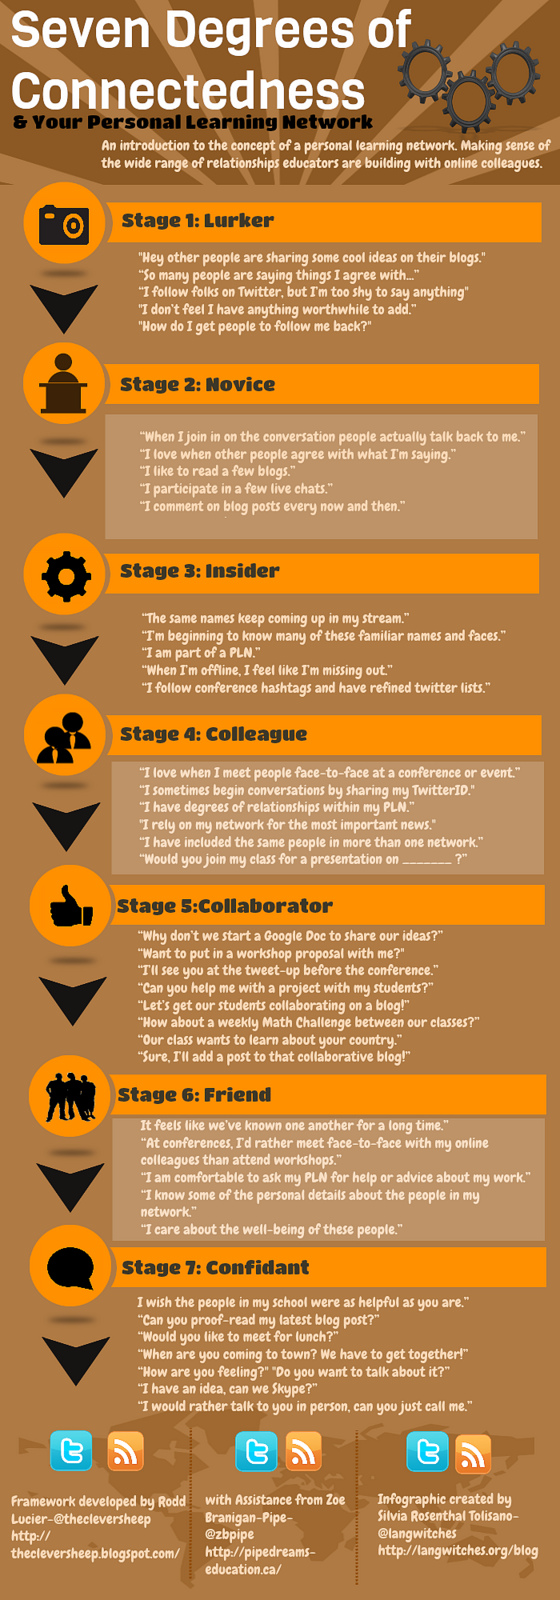
\includegraphics[width=.56\textwidth]{../pictures/k12-infographic.jpg}
\end{center}
\end{figure}
\FloatBarrier

(The figure on the previous page is licensed as CC By-NC-SA, on
 \href{http://www.flickr.com/photos/thecleversheep/7161689001/sizes/l/in/photostream/}{Flickr}.)

Consider taking the plunge into the different stages of a
Networked/Connected Educator today.

\subsection{Additional resources}

\subsubsection{amazing technology tools for your classroom:}

\begin{itemize}
\item
  \href{http://www.freetech4teachers.com/}{Richard Byrne}
\item
  \href{http://langwitches.org/blog/}{Sylvia Tolisano}
\item
  \href{http://catlintucker.com/2011/11/12-tech-tools-that-will-transform-your-classroom/}{Caitlin
  Tucker}
\item
  \href{http://coolcatteacher.blogspot.ca/}{Vicki Davis}
\end{itemize}
\subsubsection{How to develop your PLN:}

\begin{itemize}
\item
  \href{\%20http://thecleversheep.blogspot.ca/2012/06/seven-degrees-of-connectedness\_06.html}{Degrees
  of Connected Teaching} by Rodd Lucier
\item
  \href{\%20http://thecleversheep.blogspot.ca/2012/06/seven-degrees-of-connectedness\_06.html}{TeachThought}
\end{itemize}
\subsubsection{Theory \& philosophy of connnected learning for classroom
transformation:}

\begin{itemize}
\item
  \href{http://pairadimes.davidtruss.com/}{David Truss}
\item
  \href{http://www.downes.ca/presentation/264}{Steven Downes}
\item
  \href{http://willrichardson.com/}{Will Richardson}
\end{itemize}

%
\chapter[\textbf{P2P SOLE}]{P2P Self-Organized Learning Environments}
%
\attrib{Jan Herder}
%
\begin{quote}
From this conversational piece you can engage in a journey to affect
your learning space through many points of entry interacting with the
physical one.  We hope to inspire emerging structure and reciprocal
mentoring to create a ripple effect for those willing to open the door
to a new possible world.
\end{quote}

\subsection{The Guiding Strategy:}

In his \href{http://peeragogy.org/case-study-5ph1nx/}{Peeragogical Case
Study} David Preston states:

\begin{quote}
\emph{Peeragogical interaction requires refining relational and topical
critique, as well as skills in other ``meta'' literacies, including but
not limited to critical thinking, collaboration, conflict resolution,
decision-making, mindfulness, patience and compassion.} 
\sourceatright{From ``Case Study: 5PH1NX'' (this volume).}
\end{quote}

A
\href{http://en.wikipedia.org/wiki/Self\_Organised\_Learning\_Environment}{Self-Organizing
Learning Environment}, or SOLE, with a living structure accomplishes all
of these outcomes, or David's ``meta-literacies,'' simultaneously.
An authentic problem and/or project based activity in a
connected learning environment includes diverse learners in diverse ways
by empowering all learners as peers.

This provides the authentic
learning environment with which to design a SOLE. SOLEs are everywhere.
How have we evolved as a species, if not through self-organizing? A
conversation between strangers is self organizing, each learning about
something 
\clearpage
\begin{vplace}[0.5]
\noindent 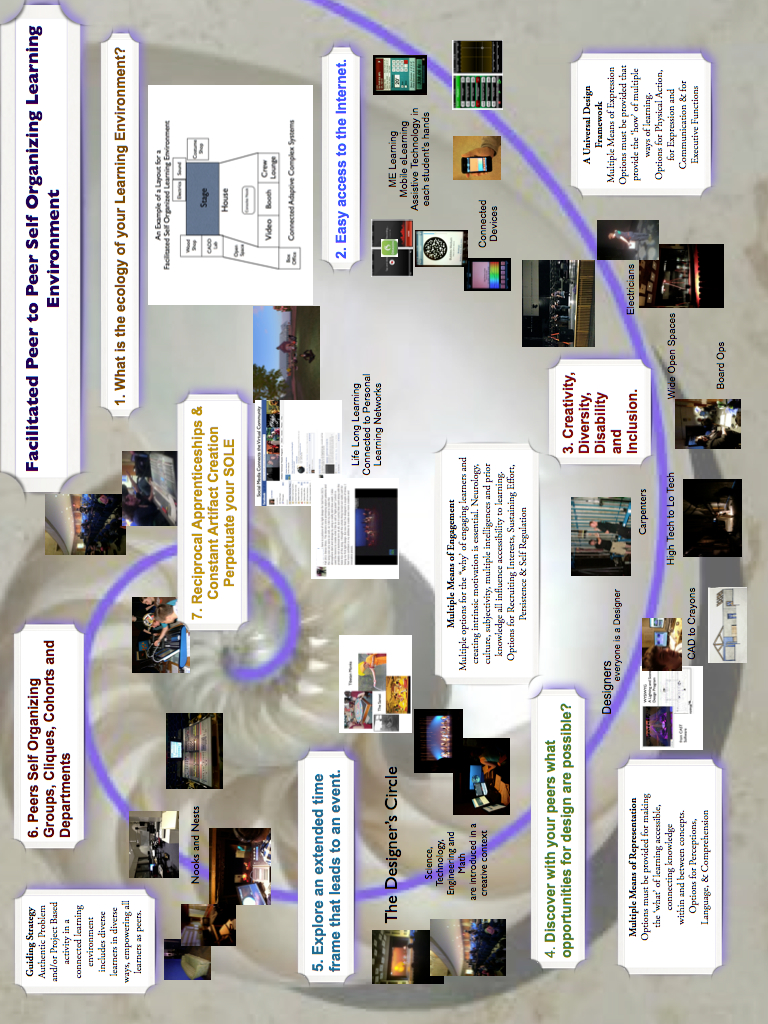
\includegraphics[width=\textwidth]{../pictures/sole-l.jpg}
A visualization of the facilitated peer to peer SOLE, full-size
at \url{http://goo.gl/7StkJK}
\end{vplace}
\clearpage

\noindent or each other. The spaces around people conversing is also an
environment, though not explicitly a learning one. While we are always
self-organizing to learn or accomplish things, one place that SOLEs do
not always exist are in learning institutions. In many educational
institutions, our learning environments are predominately organized by
the teacher, curriculum, or society. How can we nurture peer to peer
learning environments to organize? How does the role of the teacher
differ in a SOLE? In what ways can we unite that fundamental, passionate
human characteristic of curiosity and self-organizing back into our
Learning Environments? 

The model that
\href{http://sugatam.wikispaces.com/}{Sugata Mitra} {[}2{]} is
experimenting with gives us some scaffolding to create one ourselves.
This is the goal of his
\href{http://www.ted.com/pages/sole\_toolkit}{SOLE Tool Kit} (3).
Sugata's kit is directed towards children between 8 and 12 years old. I
was wondering if there is a way to make it more universal in its
application. How can I apply it to my situation? How is a SOLE different
in the context of peer to peer learning? This chapter of the Handbook
uses Sugata's model as a doorway into our understanding a SOLE approach
to peer to peer learning. Its three key components are: learners,
context and project. I find the discussion needs to integrate what we
are learning about diverse learners into a
\href{http://www.udlcenter.org/aboutudl/udlguidelines}{Universal Design
for Learning} {[}4{]} context. After all, we cannot take for granted who
the peers are in the SOLE. Equally, the context, the learning
environment (LE) must be as deeply considered as the learners
participating. As a learning designer, I am also seeking more clues
about the living structure of a well crafted SOLE.

\subsection{Centers within the Center}

SOLEs exist in a particular context. Take Sugata's
\href{http://www.ted.com/talks/sugata\_mitra\_shows\_how\_kids\_teach\_themselves.html}{hole
in the wall} {[}5{]} experiment. The parameters of the environment of a
computer embedded in a wall in India are very specific. Sugata's act was
to design a project in order to facilitate a process within that
environment. The elements he introduced were a touch screen computer
embedded in a wall with specific software. Sugata has abstracted this
design into a Tool Kit. He speaks of `Child Driven Learning',
intrinsically motivated learning with the curiosity to learn something
in particular. As a learner-centric peeragogy, SOLEs are emergent,
bottom up, seeking to answer: How do we design a project (or
phrase a problem) that ignites a learner's passion?

A SOLE is a
facilitated learning environment (LE) that can nurture learner driven
activity. For instance, in the Hole in the Wall example, the design is
the context of the wall, the street, the neighborhood --and the
facilitation is the touch screen monitor in the wall. They are
brilliantly united. In this sense it is an intentional, self-aware
learning environment. It is a strange foreign object that anyone would
have to figure out how it works to take advantage of. But this is not in
the classroom, or in the `school.' It is an informal LE. Just
like
\href{http://www.academia.edu/1137269/Game-based\_Learning\_and\_Intrinsic\_Motivation}{learning
a game} {[}6{]}, there is an entire ecology that surrounds you. This is
very much a systemic approach. The context is facilitated explicitly
(your design of the SOLE), but also implicitly in the
\href{http://en.wikipedia.org/wiki/Hidden\_curriculum}{hidden
curriculum} {[}7{]} that defines your LE. Above is the layout of the
\href{http://www.scribd.com/doc/181089012/Transformed-Learning-Environment-Analysis}{transformed
learning environment} {[}8{]} I explored to work around the hidden
curriculum of the traditional classroom. The LE has a tremendous, if not
\href{http://scholar.lib.vt.edu/theses/available/etd-09232007-220306/unrestricted/SElmasryETDbodytext.pdf}{overwhelming
influence, on learning} {[}9{]}. The first step in connected learning is
to reconnect to the environment around us. For me, the primary context
of my LE is a performing arts center at a small rural liberal arts
college. The Performing Arts Center is a Center within the context of
the college and community. A diversity of spaces within the facility are
inhabited: small and cozy, large and public, technology embedded
everywhere, all focused on the project based learning that emerges
producing a performance. I stay away from a formal classroom as much as
possible. These spaces are Centers within the Center,
`\href{http://nourdiab.wordpress.com/2011/02/23/the-theories-of-christopher-alexander/}{loosely
connected adaptive complex systems}' {[}10{]} within themselves, just
like people. I believe that the possibility of a SOLE emerging as a
living structure seems to depend on the correct types of complex systems
engaged in the LE.

What is the role of the internet in your design? Mitigating inequalities
and accommodating diverse learners are somewhat assisted by access to
the internet. But it is the immediate,
\href{http://www.wordstream.com/blog/ws/2013/10/02/just-in-time-information-hacks}{just-in-time
learning} {[}11{]} that makes free and open access to the world wide web
so important in a SOLE. Wireless is available throughout this LE. Nooks
and lounges, interconnected, but separate rooms, provide lots of places
for collaboration or solitary work, for staying connected or hiding out.
In a UDL vision of a facilitated peer to peer SOLE, technology is
integral to the design. In the case of my LE, with the use of digital
audio, multi-media, database management, robotic lighting and
\href{http://en.wikipedia.org/wiki/Dichroic\_filter}{dichroic} {[}12{]}
colors, learners are accustomed to accessing and augmenting reality with
technology: allowing learners to access their social media is part of
their content creation.

Do we start our SOLE as peers? Peer to peer assumes your participants
are peers--especially you, the facilitator. There needs to be enough
diversity and complexity to include all learners, engendering a
\href{http://www.cast.org/library/UDLguidelines/}{Universally Designed
Context} {[}13{]}. What is the role of diversity in peer to peer SOLE
building? How are diverse learners peers? In my LE, I discovered 70\% of
my learners have learning challenges. I know my LE is not unique in this
regard. I have to facilitate a SOLE design that is inclusive. This is in
contradistinction to commonality, yet this diversity is what we crave,
for creativity and innovation, for deep learning to occur. Crafting your
SOLE using multiple means of representation, expression and engagement
empowers learners to be peers. A diverse learning environment,
supporting diverse learning styles and diverse learners, supports a
complex project based SOLE. But there are many SOLEs within the SOLE
since learning is occurring on many levels with each student and within
each group. We do not all get the same thing at the same time. Learning
outcomes are diverse, emergent, serendipitous.

What type of project, problem or event will focus your efforts? Either a
\href{http://www.theatreprof.com/2011/active-learning-student-generated-syllabus/}{learner
generated syllabus {[}}14{]} may emerge from the SOLE, or a
\href{http://usergeneratededucation.wordpress.com/}{user generated
education} {[}15{]} within a specific context may answer this question.
Ownership and leadership emerge when learners can apply their creativity
and/or authentically assist each other in a common goal. Opportunities
to design and modify even small things will draw learners into a
project. The more they must rely on each other, collaborate and share
their creativity, their designs and actualization--the more they work
together as peers. The spaces in your LE are most likely already
designed and built to accommodate the purpose of the facility in the
context of the college or school. We cannot really redesign the actual
space, but we can redesign many aspects. We can look for designs within
it. Being able to design your own space, or project, is critical to
taking ownership of your learning and experiencing the consequences. As
learners mature and look for ways to be more involved, I suggest they
redesign the shop, the repertory lighting plot, or the procedures of
their department and/or SOLE overall. Exchanging roles as designer also
stimulates peer interaction. Why not integrate design and design
thinking? In my context, lighting, scene, costume and sound design are
interconnected opportunities. Along with accompanying technology, every
opportunity is used to nurture empathy, creativity, rationality and
systems thinking. Integral to the learner generated syllabus or project
design should be continuous artifact creation. A great place to start
the design process and to begin to generate content is by using a
virtual world.

Constant content creation can integrate assessment into your SOLE. It is
the quality of the artifacts created along the way that reveals the
success of your SOLE. Media that chronicles a journey through time,
created by each learner, reveals the depth of participation. It is
nearly impossible to cheat. The learner expresses their comprehension in
the types and extent of artifact creation.

As the facilitator, I look for opportunities to introduce the
unexpected, bigger questions, deeper considerations, along the way. For
example, in the context of my LE, one of the events feature Tibetan
Monks. They bring a counterpoint to the inflated egos and cult of
personality which is prevalent in our context. The SOLE Plan is
extended. It can happen over a much longer amount of time than one class
or one day. The actors rehearse for weeks, as the design team designs,
giving time for: research, absorption, misleads, mistakes, correction
and reflection. A SOLE needs time and persistence to generate artifacts,
documentation and experiences of the project and virtual worlds are an
excellent way to extend time and space synchronously and asynchronously.

Sugata emphasizes the Big questions. We do not always know what they
are. A focus? A goal? A product? And the event? That should be decided
with the group. The learners intuit the direction that leads to deep
engagement and the bigger questions. I try and leave it ambiguous,
suggesting some of the things they might encounter. Facilitating the
SOLE in this context, we face endless questions connected to the
specific LE, to all the imaginary scenarios, Herculean tasks and
questions-- like building castles, programming a digital sound console,
troubleshooting robotic lighting instruments, how to make the illusion
of fire or, even, who killed Charlemagne? The Box Office is an example
of an informal SOLE that has emerged recurrently over time. I have
noticed that its vitality depends on the characters and the ebb and flow
of learners entering the group or graduating. The physical space is a
small, windowless and often damp room with a couple of couches and a
desk with a computer squeezed in. My very own `Hole in the Wall'
experiment. The bottom of the door can remain closed, while the top is
open, like a stable. Primarily the students are paid to be there,
answering the phone, reserving tickets, greeting patrons and managing
the Box Office and the Front of the House. In the SOLE, this subtle
inversion of the institutional value proposition turns `work study' into
studying work. This is an informal LE nested within the context of the
formal institution and the wider LE: a center within a center. Some
semesters there are business majors working their way up the job ladder:
Usher to Assistant Front of House Manager, to Assistant Box Office
Manager, to Box Office Manager. Sometimes this takes 4 years, sometimes
it happens in a semester or two. It is a recursive SOLE that differs as
the interests and skills of the students who inhabit the space change.
As the current manager puts it, the Box Office is a `constantly evolving
puzzle.'

This example of a SOLE in an informal LE is similar to the other types
of SOLE's that occur within a facilitated LE. The learner's interact as
reciprocal apprentices, leaning on one another to solve challenges and
problems. Groups are self-selective, this type of work suits their
temperament and interests, or time. This cohort is almost a clique,
attracting their boyfriends and girlfriends. They begin initiatives,
re-design the lobby for crowd control, redecorate and rearrange the
space constantly, decide their schedules and split up responsibility.
Everyone is always training everyone, because the environment turns over
each semester. It is explicitly an informal LE. The workers are
students. This inverts the usual state of affairs, where essentially
they are being paid to learn, though they may not even be aware of it.
Occasionally, the learning experience resonates deeply with them. A
number of them have used the experience to leverage jobs that parallel
their interests, or get them started on their careers. 

Job
titles, roles of responsibility, are often problematic in a SOLE. The
bottom line is that as peers we are all equal and at certain times
everyone is expected to do everything regardless of their roles. Titles
go to people's heads. But this is part of the experience. Keep the
titles moving, change it up when things get bottlenecked over
personalities. Sometimes I create duplicate positions, Assistants of
Assistants. and Department Heads. The Apprenticeship model is at play
but in a new way in a SOLE. There are peers and there are peers. As
power struggles emerge, some like-to-like grouping occurs. The role of
the facilitator becomes mediator. The emergent epistemology of abundance
and connected learning asks for a multitude of `experts.' In the same
way, leadership can be distributed, flowing as varying needs arise.

The experience of practicing leadership skills and encountering all the
variables of working with diverse folks quickly gives feedback to us if
this is a helpful role for this person. It is messy sometimes, and there
are conflicts. After a few events, they learn how to manage a Box
Office, dealing with patrons, emergencies, complaints and bag check.
They confront the larger peer group, the student body, with authority
and empathy. They are very proud of their jobs and make their own name
tags with titles. A hierarchy gives them rewards that they have been
trained to expect from years in school. It is another way of developing
intrinsic motivation and challenges them to interact with their peers
authentically. 

As facilitator, I try to leave them alone as much
as possible. The context has been created, the computer in the wall is
on a desk. Extending the design of your SOLE contributes to its living
structure. I have used
\href{http://community.telecentre.org/profiles/blogs/facebook-as-a-supplemental-lms}{Facebook
as a Supplemental LMS} {[}16{]} since 2007 because this is where my
students are and it allows them to control the structures of groups
emergently. The learners create the groups as they are relevant. The
facilitator does not. Usually they invite me in! For now, Facebook
aggregates the learning community that the SOLE inspires as learners
become leaders, establish connections with each other and mentor
newbies. This activity is integrated into artifact creation, `comments'
and documentation of their personal learning journey. Facebook becomes a
precursor for their portfolios, and in some cases, it is their
portfolio.
\href{http://starwars.wikia.com/wiki/Reciprocal\_apprenticeship}{Reciprocal
Apprenticeships} {[}17{]} occur in the dynamic of collaboration among
peers. Continuity in time beyond the event horizon is accomplished by
these relationships. Peers nurture one another along the shared learning
journey that the SOLE provides. As facilitator and designer, you are,
most of all, in a reciprocal relationship with the other learners. This
is the essence of being a peer, an interaction that respects what each
of us brings to the experience.

\subsection{A review}

\begin{quote}
\textbf{Sugata Mitra}: It is great to see the thinking that has gone into taking the idea of a SOLE forward. To my mind, SOLEs are quite experimental at this time and efforts such as these will provide invaluable data. I look forward to this. I notice that most of the important design features of a SOLE are incorporated into the article. I repeat them anyway, just to emphasise:
\begin{enumerate}
\item Large, publicly visible displays are very important, this is what resulted in the surprising results in the hole in the wall experiments and subsequent SOLEs for children in England and elsewhere.
\item The absence of unnecessary people in the learning space, no matter who they are; parents, teachers, principals, curious adults etc.
\item Free, undirected activity, conversation and movement.
\item A certain lack of order: I must emphasise that ‘Self Organised’, the way I use it does not mean ‘organising of the self’. Instead it has a special meaning from the subject, Self Organising Systems, a part of Chaos Theory. The SOLE should be a space at the ‘edge of chaos’, thereby increasing the probability of the appearance of ‘emergent order’.
\end{enumerate}
\end{quote}

\subsection{References}

\begin{enumerate}
\item
  Preston, David (2014). \href{http://peeragogy.org/case-study-5ph1nx/}{Case Study:
  5PH1NX} (pp. \pageref{sphinx-beginning}--\pageref{sphinx-end}, this volume).
\item
  \href{http://sugatam.wikispaces.com/}{About Sugata Mitra}, on Wikispaces.
\item
  \href{http://www.ted.com/pages/sole\_toolkit}{The SOLE Toolkit}, on TED.com.
\item National Center for Universal Design for Learning,
  \href{http://www.udlcenter.org/aboutudl/udlguidelines}{Universal Design for
  Learning Guidelines}.
\item Sugata Mitra (2010).
  \href{http://www.ted.com/talks/sugata\_mitra\_the\_child\_driven\_education.html}{The child-driven education}, TED.
\item
  \href{http://www.academia.edu/1137269/Game-based\_Learning\_and\_Intrinsic\_Motivation}{Game-based
  Learning and Intrinsic Motivation by Kristi Mead}.
\item
  \href{http://en.wikipedia.org/wiki/Hidden\_curriculum}{Hidden Curriculum}, on Wikipedia.
\item
  \href{http://www.scribd.com/doc/181089012/Transformed-Learning-Environment-Analysis}{Transformed
  Learning Environment Analysis}, by Jan Herder (on ScribD).
\item
  Elmasry, Sarah Khalil (2007). \href{http://scholar.lib.vt.edu/theses/available/etd-09232007-220306/unrestricted/SElmasryETDbodytext.pdf}{Integration
  Patterns of Learning Technologies}. IRB\# 05-295-06.
\item
  Curious: \href{http://nourdiab.wordpress.com/2011/02/23/the-theories-of-christopher-alexander/}{In-Forming
  singular/plural design, The Theories of Christopher Alexander}.
\item
  \href{http://www.wordstream.com/blog/ws/2013/10/02/just-in-time-information-hacks}{Overwhelmed
  with Blog Tips? Hack Learning with Just In Time Information}, on Wordstream.com.
\item
  \href{http://en.wikipedia.org/wiki/Dichroic\_filter}{Dichroic Filter}, on Wikipedia.
\item \href{http://www.cast.org/library/UDLguidelines/}{UDL Guidelines} on cast.org.
\item
  \href{http://www.theatreprof.com/2011/active-learning-student-generated-syllabus/}{Active
  Learning Student Generated Syllabus}, on theatreprof.com.
\item
  \href{http://usergeneratededucation.wordpress.com/}{User Generated
  Education Blog} on wordpress.com.
\item
  \href{http://community.telecentre.org/profiles/blogs/facebook-as-a-supplemental-lms}{Facebook
  as a Supplemental LMS}, on telecentre.org.
\item
  \href{http://starwars.wikia.com/wiki/Reciprocal\_apprenticeship}{Reciprocal
  Apprenticeship}, on Star Wars Wikia.
\end{enumerate}

%
\chapter[\textbf{A story about new beginnings}]{A story about new beginnings}
%
Once he gets to the Whispering Gallery, Jorge realizes that the girl was
right. This \emph{is} the center of the universe. There are murmurs to
be heard there -- it seems they come from everywhere. He hears about
guilds and the craftsmen who built the cathedral. He learns about how
proud they were and how they formed communities of practice, educating
the uninitiated, teaching each other to create. He returns to ground
level. The girl is gone, but he feels happy and inspired.~ He can do
much more then repackage social media streams; there is more going on
here than Twitter as a new broadcast medium.~ He starts a new journey:
finding a guild, a community of practice, but restyled in a 21st century
fashion.~ It will be more open, more connected to others then the old
guilds. He will still use Twitter, a social dashboard, and curating
tools, but also he uses wikis, and synchronous communication.~ And most
importantly, he starts building, together with others -- in particular,
together with the people formerly known as his readers. They will
co-create the analysis, the search for solutions and sense-making,
rather than helplessly listening to ``experts'', passively consuming
pre-processed knowledge and information. Instead, they'll start building
their own destiny, and the newsroom will be part of the platform.
{[}caption id=``'' align=``aligncenter''
width=``520''{]}\href{http://peeragogy.org/a-story-of-beginnings/section/}{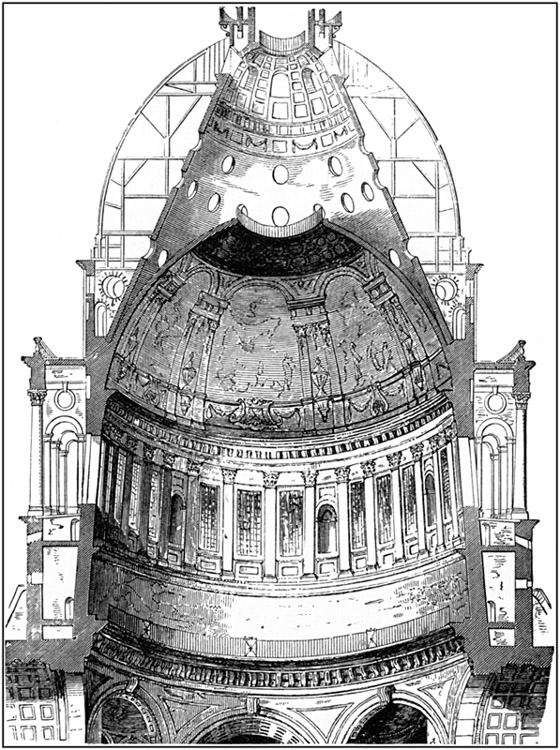
\includegraphics{http://peeragogy.org/wp-content/uploads/2013/12/section.jpg}}
Section of the Dome at St Paul's Cathedral{[}/caption{]}




\part{Organizing a Learning Context} \label{organizing-part} %%%%%%%%%%%%%%%%%%%%
%
\chapter[\textbf{Organizing Co-Learning}]{Introduction to Organizing Co-Learning}
This section about organizing Co-Learning rests on the assumption that
learning always happens in a context, whether this context is a
structured ``course'' or a (potentially) less structured ``learning
space''. For the moment we consider the following division:

\begin{itemize}
\item
  \emph{Organizing Co-learning Contexts}

  \begin{itemize}
  \item
    Courses (= ``learning linked to a timeline or syllabus'')
  \item
    Spaces (= ``learning not necessarily linked to a timeline or
    syllabus'')
  \end{itemize}
\end{itemize}

This section focuses on existing learning contexts and examines in
detail how they have been ``organized'' by their (co-)creators. (See
also:
\href{http://socialmediaclassroom.com/host/peeragogy/wiki/structural-dimensions-the-what-we-are-learning-vs-time-and-types-structures}{the
structural dimensions of group formation}.)

At a ``meta-level'' of media, we can talk about this parallel structure:

\begin{itemize}
\item
  \emph{Building Co-learning Platforms}

  \begin{itemize}
  \item
    Development trajectories (e.g. ``design, implement, test, repeat'')
  \item
    Platform features (e.g. forums, wikis, ownership models, etc.)
  \end{itemize}
\end{itemize}

A given learning environment with have both time-like and space-like
features as well as both designed-for and un-planned features. A given
learning platform will encourage certain types of engagement and impose
certain constraints. The question for both ``teachers'' and ``system
designers'' -- as well as for learners -- should be: \emph{what features
best support learning?}

The answer will depend on the learning task and available resources.

For example, nearly everyone agrees that the best way to learn a foreign
language is through immersion. But not everyone who wants to learn, say,
French, can afford to drop everything to go live in a French-speaking
country. Thus, the space-like full immersion ``treatment'' is frequently
sacrificed for course-like treatments (either via books, CDs, videos, or
ongoing participation in semi-immersive discussion groups).

System designers are also faced with scarce resources: programmer time,
software licensing concerns, availability of peer support, and so forth.
While the ideal platform would (magically) come with solutions
pre-built, a more realistic approach recognizes that problem solving
always takes time and energy. The problem solving approach and
associated ``learning orientation'' will also depend on the task and
resources at hand. The following sections will develop this issue
further through some specific case studies.

\subsection{\emph{Case study 1 (pilot, completed)}: ``Paragogy'' and the
After Action Review.}

In our analysis of our experiences as course organizers at P2PU, we (Joe
Corneli and Charlie Danoff) used the US Army's technique of After Action
Review (AAR). To quote from
\href{http://paragogy.net/ParagogyPaper2}{our paper} {[}2{]}:

\begin{quote}
As the name indicates, the AAR is used to review training exercises. It
is important to note that while one person typically plays the role of
evaluator in such a review {[}\ldots{}{]} the review itself happens
among peers, and examines the operations of the unit as a whole.

The four steps in an AAR are:

\begin{enumerate}
\item
  Review what was supposed to happen (training plans).
\item
  Establish what happened.
\item
  Determine what was right or wrong with what happened.
\item
  Determine how the task should be done differently the next time.
\end{enumerate}

The stated purpose of the AAR is to ``identify strengths and
shortcomings in unit planning, preparation, and execution, and guide
leaders to accept responsibility for shortcomings and produce a fix.''
\end{quote}

We combined the AAR with several principles (see Discussion section
below), which we felt described effective peer learning, and went
through steps 1-4 for each principle to look at how well it was
implemented at P2PU. This process helped generate a range of advice that
could be applied at P2PU or similar institutions. By presenteding our
paper at the \href{http://okfn.org/okcon/}{Open Knowledge Conference
(OKCon)}, we were able to meet~P2PU's executive director, Philipp
Schmidt, as well as other highly-involved P2PU participants; our
feedback may have contributed to shaping the development trajectory for
P2PU.

In addition, we developed a strong prototype for constructive engagement
with peer learning that we and others could deploy again. In other
words, variants on the AAR and the paragogical principles could be
incorporated into future learning contexts as platform features {[}3{]}
or re-used in a design/administration/moderation approach {[}4{]}.~ For
example, we also used the AAR to help structure our writing and
subsequent work on \href{http://paragogy.net}{paragogy.net}.

\subsection{\emph{Case Study 2 (in progress)}: ``Peeragogy''.}

Our particular focus in the interviews was on drawing out and
emphasizing the relational dimension of students, learning experiences
within their environment and, consequently, on inferring from their
accounts a sense of how they perceived and indeed constituted their
environment. We asked them who they learned with and from and how. A
further question specifically focused on whom they regarded as their
peers and how they understood their peers as a source and a site for
learning." {[}1{]}

In this section, we will interview and/or survey members of the
Peeragogy community with questions similar to those used by Boud and Lee
{[}1{]} and then identify strengths and shortcomings as we did with the
AAR above. These questions are derived from the AAR.

\textbf{Questions} (discussed on an
\href{https://peeragogy.etherpad.mozilla.org/7}{etherpad}; revisions to
the original set of questions are marked in italics):

\begin{enumerate}
\item
  Who have you learned with \emph{or} from in the Peeragogy project?
  \emph{What are you doing to contribute to your peers' learning?}
\item
  How have you been learning during the project?
\item
  Who are your peers in this community, and why?
\item
  What were your expectations of participation in this project?
  \emph{And, specifically, what did you (or do you) hope to learn
  through participation in this project?}
\item
  What actually happened during your participation in this project (so
  far)? \emph{Have you been making progress on your learning goals (if
  any; see prev. question) -- or learned anything unexpected, but
  interesting?}
\item
  What is right or wrong with what happened (Alternatively: how would
  you assess the project to date?)
\item
  How might the task be done differently next time? (What's ``missing''
  here that would create a ``next time''\emph{, ``sequel'', or
  ``continuation''?})
\item
  \emph{How would you like to use the Peeragogy handbook?}
\item
  \emph{Finally, how might we change the questions, above, if we wanted
  to apply them in your peeragogical context?}
\end{enumerate}

\subsubsection{\textbf{Reflections on participants' answers}}

The questions were intended to help participants reflect on, and change,
their practice (i.e. their style of participation). There is a tension,
however, between changing midstream and learning what we might do
differently next time. There is a related tension between initial
structure and figuring things out as we go. Arguably, if we knew, 100\%,
how to do peeragogy, then we would not learn very much in writing this
handbook. Difficulties and tensions would be resolved ``in advance''
(see earlier comments about ``magical'' technologies for peer
production).

And yet, despite our considerable collected expertise on collaboration,
learning, and teaching, there have been a variety of tensions here!
Perhaps we should judge our ``success'' partly on how well we deal with
those. Some of the tensions highlighted in the answers are as follows:

\begin{enumerate}
\item
  \emph{Slow formation of ``peer'' relationships.} There is a certain
  irony here: we are studying ``peeragogy'' and yet many respondents did
  not feel they were really getting to know one another ``as peers'', at
  least not yet. Those who did have a ``team'' or who knew one another
  from previous experiences, felt more peer-like in those relationships.
  Several remarked that they learned less from other individual
  participants and more from ``the collective'' or ``from everyone''. At
  the same time, some respondents had ambiguous feelings about naming
  individuals in the first question: ``I felt like I was going to leave
  people out and that that means they would get a bad grade - ha!'' One
  criterion for being a peer was to have built something together, so by
  this criterion, it stands to reason that we would only slowly become
  peers through this project.
\item
  \emph{``Co-learning'', ``co-teaching'', ``co-producing''?} One
  respondent wrote: ``I am learning about peeragogy, but I think I'm
  failing {[}to be{]} a good peeragog. I remember that Howard {[}once{]}
  told us that the most important thing is that you should be
  responsible not only for your own learning but for your peers'
  learning. {[}\ldots{}{]} So the question is, are we learning from
  others by ourselves or are we {[}\ldots{}{]} helping others to
  learn?'' Another wrote: ``To my surprise I realized I could contribute
  organizationally with reviews, etc. And that I could provide some
  content around PLNs and group process. Trying to be a catalyst to a
  sense of forward movement and esprit de corps.''
\item
  \emph{Weak structure at the outset, versus a more ``flexible''
  approach.} One respondent wrote: ``I definitely think I do better when
  presented with a framework or scaffold to use for participation or
  content development. {[}\ldots{}{]} (But perhaps it is just that I'm
  used to the old way of doing things).'' Yet, the same person wrote:
  ``I am interested in {[}the{]} applicability {[}of pæragogy{]} to new
  models for entrepreneurship enabling less structured aggregation of
  participants in new undertakings, freed of the requirement or need for
  an entrepreneurial visionary/source/point person/proprietor.'' There
  is a sense that some confusion, particularly at the beginning, may be
  typical for peeragogy. With hindsight, one proposed ``solution'' would
  be to ``have had a small group of people as a cadre that had met and
  brainstormed before the first live session {[}\ldots{}{]} tasked
  {[}with{]} roles {[}and{]} on the same page''.
\item
  \emph{Technological concerns.} There were quite a variety, perhaps
  mainly to do with the question: how might a (different) platform
  handle the tension between ``conversations'' and ``content
  production''? For example, will Wordpress help us ``bring in'' new
  contributors, or would it be better to use an open wiki? Another
  respondent noted the utility for many readers of a take-away PDF
  version. The site (peeragogy.org) should be ``{[}a{]} place for people
  to share, comment, mentor and co-learn together in an ongoing
  fashion.''
\item
  \emph{Sample size.} Note that answers are still trickling in. How
  should we interpret the response rate? Perhaps what matters is that we
  are getting ``enough'' responses to make an analysis. One respondent
  proposed asking questions in a more ongoing fashion, e.g., asking
  people who are leaving: ``What made you want to quit the project?''
\end{enumerate}

With regard to Points 1 and 2, we might use some ``icebreaking''
techniques or a ``buddy system'' to pair people up to work on specific
projects. The project's ``teams'' may have been intended to do this, but
commitment or buy-in at the team level was not always high (and in many
cases, a ``team'' ended up being comprised of just one person). It does
seem that as the progress has progressed, we have begun to build tools
that could address Point 3: for example, the Concept Map could be
developed into a process diagram that would used to ``triage'' a project
at its outset, help project participants decide about their roles and
goals. Point 4 seems to devolve to the traditional tension between the
``good enough'' and the ``best'': we have used an existing platform to
move forward in an ``adequate'' way. And yet, some technological
improvements may be needed for future projects in pæragogy.
(Furthermore, note that our choice to use a CC0 license means that if
other people find the content useful, they are welcome to deploy it on
their own platform, if they prefer.) Finally, Point 5 is still up in the
air (more answers more be coming in shortly - I think I have sent around
enough reminders). Hopefully the questionnaire will be useful to the
group even with a not-100\% response rate! Points 4 and 5 are related,
in that an ongoing questionnaire for people leaving (or joining) the
project could be implemented as a fairly simple technology, which would
provide feedback for site maintainers. Gathering a little information as
a condition of subscribing or unsubscribing seems like a safe,
light-weight, way to learn about the users (tho there is always the
possibility that rather than unsubscribing, non-participating users will
just filter messages from the site).

An underlying tension (or synergy?) -- between learning and producing --
was highlighted in our earlier work on paragogy. If we learn by
producing, that is good. However, I have argued in {[}4{]} that
paragogical praxis is based less on producing and more on reusing. If
downstream users of this handbook find it to, indeed, be useful, we may
have done enough. \emph{For all we know, we are the ``cadre'' (see
above) charged with determining how best to do things in ``subsequent
rounds''!}And, with this, we turn to a third case study, where our work
so far is reapplied in an offline educational context.

\subsection{Discussion}

We reconsider the appropriateness of the AAR and the paragogy principles
in contexts beyond P2PU, using Lisewski and Joyce as a guide to our
(meta-)critique and analysis.

\begin{quote}
\emph{In recent years, the tools, knowledge base and discourse of the
learning technology profession has been bolstered by the appearance of
conceptual paradigms such as the `five stage e-moderating model'
(Salmon, 2000) and the new mantra of `communities of practice' (Wenger,
1998). This paper will argue that, although these frameworks are useful
in informing and guiding learning technology practice, there are
inherent dangers in them becoming too dominant a discourse. The main
focus will be on the `five stage e-moderating model' as providing an
exemplar of a discourse which is in danger of forming a `grand
narrative' (Lyotard, 1984) or totalizing explanation of how to design
and deliver online training programmes.} -- Lisewski and Joyce
\end{quote}

In a sense, the more reified a pattern, the less we learn by deploying
it
(\href{http://socialmediaclassroom.com/host/peeragogy/forum/anti-patterns-concerns-complaints-and-critiques\#comment-2355}{see
these comments}).~If we were trying to validate the paragogy model
simply by fitting feedback to it (Case Study 2), that would be an act of
intellectual dishonesty. Nevertheless, the act of fitting data to this
model, as a constructive and creative act, is in fact useful -- and a
sign that we are still learning about what makes paragogy work. Not only
on a theoretical level (summed up below), but also on a technological
level (see
\href{http://socialmediaclassroom.com/host/peeragogy/wiki/researching-p\%C3\%A6ragogy}{this
page}).

{\footnotesize
\ctable[pos = H, center, botcap]{p{.5\textwidth}p{.5\textwidth}}
{% notes
}
{% rows
\FL
\textbf{Paragogical Principles\ldots{}} & \textbf{Reflections on
practice and experience suggest\ldots{}}
\\\noalign{\medskip}
1. \emph{Changing context as a decentered center.} We interact by
changing the space. & 1. \textbf{Develop empirical studies and a
critical apparatus.}\textbf{}\emph{It seems we begin with \emph{w}eak
ties, and then experience a slow formation of ``peer'' relationships, as
we form and re-form our social context, and come to better understand
our goals.}
\\\noalign{\medskip}
2. \emph{Meta-learning as a font of knowledge.} We interact by changing
what we know about ourselves. & 2. \textbf{Find companions for the
journey}. \emph{We learn a lot about ourselves by interacting with
others. But participants struggle to find the right way to engage:}
\emph{``co-learning'', ``co-teaching'', or ``co-producing''? Moreover,
``People come--they stay for a while, they flourish, they build--and
they go.''}
\\\noalign{\medskip}
3. \emph{Peers provide feedback that wouldn't be there otherwise.} We
interact by changing our perspective on things. & 3. \textbf{Work with
real users}. \emph{We begin with a weak structure at the outset but this
may afford a more ``flexible'' approach as time goes on (see also this
\href{http://peeragogy.org/adding-structure-with-activities/}{handbook
section} which offers advice on designing activities that help create a
``flexible structure'').}
\\\noalign{\medskip}
4. \emph{Learning is distributed and nonlinear.} We interact by changing
the way things connect. & 4. \textbf{Study and build nonlinear
interfaces}. \emph{There are a number of technological concerns, which
in a large part have to do with tensions between ``content production''
and ``conversation'', and to a lesser extent critique the platforms
we're using.}
\\\noalign{\medskip}
5. \emph{Realize the dream if you can, then wake up!} We interact by
changing our objectives. & 5. \textbf{Limit philosophizing}. E\emph{ven
with a small group, we can extract meaningful ideas about peer learning
and form a strong collective effort, which moves things forward for
those involved: this means work. We would not get the same results
through ``pure contemplation''.}
\LL
}}

This table seems to suggests that paragogy is less of a grand narrative
and more of a patchwork collection of tricks or heuristics for group
work. Rather than narrativizing peer learning, paragogy itself provides
a non-linear interface that we can plug into and adapt where appropriate
(like we adapted our questionnaire's questions in Case Study 2). Instead
of one grand narrative, we see a growing collection of
"\href{http://socialmediaclassroom.com/host/peeragogy/wiki/patterns-and-use-cases}{use
cases}``. The more we share our practice and experience having to do
with co-organizing learning or building platforms for the same, the more
robust and useful paragogy will become. It may never become a''rigorous
discipline"! But if not, that is OK.

\subsection{References}

\begin{enumerate}
\item
  Boud, D. and Lee, A. (2005).
  \href{http://manainkblog.typepad.com/faultlines/files/BoudLee2005.pdf}{`Peer
  learning' as pedagogic discourse for research education}.
  \emph{Studies in Higher Education}, 30(5):501--516.
\item
  Joseph Corneli and Charles Jeffrey Danoff,
  \href{http://ceur-ws.org/Vol-739/paper\_5.pdf}{Paragogy}, in Sebastian
  Hellmann, Philipp Frischmuth, Sören Auer, and Daniel Dietrich (eds.),
  \emph{Proceedings of the 6th Open Knowledge Conference, Berlin,
  Germany, June 30 \& July 1, 2011},
\item
  Joseph Corneli and Alexander Mikroyannidis (2011).
  \href{http://greav.ub.edu/der/index.php/der/article/view/188/330}{Personalised
  and Peer-Supported Learning: The Peer-to-Peer Learning Environment
  (P2PLE)}, \emph{Digital Education Review}, 20.
\item
  Joseph Corneli,
  \href{http://paragogy.net/ParagogicalPraxisPaper}{Paragogical Praxis},
  to appear in \emph{E-Learning and Digital Media} (ISSN 2042-7530),
  Volume 9, Number 3, 2012
\item
  Lisewski, B., and P. Joyce (2003). Examining the Five Stage
  e-Moderating Model: Designed and Emergent Practice in the Learning
  Technology Profession, \emph{Association for Learning Technology
  Journal}, 11, 55-66.
\end{enumerate}

%
\chapter[\textbf{Adding structure}]{Adding structure with activities}
%
In the introduction to ``Organizing a Learning Context'', we remarked
that a ``learning space'' is~\emph{only potentially}~less structured
than a ``course''. ~For example, a library tends to be highly
structured, with quiet rooms for reading, protocols for checking out
books, a cataloging and shelving system that allows people to find what
they are looking for, as well as rules that deter vandalism and theft.
(Digital libraries don't need to play by all the same rules, but are
still structured.)

But more structure does not always lead to better learning. In a 2010
Forbes article titled, ``The Classroom in 2020,'' George Kembel
describes a future in which ``Tidy lectures will be supplanted by messy
real-world challenges.'' The Stanford School of Design, (or ``d.school''
-- which Kemble co-founded and currently directs) is already well-known
for its open collaborative spaces, abundant supply of Post-It notes and
markers, and improvisational brainstorm activities -- almost the
opposite of traditional lecture-based learning.

One ``unexpected benefit'' of dealing with real-world challenges is that
we can change our approach as we go. ~This is how it works in peer
learning: peers can decide on different structures not just once (say,
at the beginning of a course), but throughout the duration of their time
together. This way, they are never ``stuck'' with existing structures,
whether they be messy or clean. At least\ldots{} that's the ideal.

In practice, ``bottlenecks'' frequently arise. ~For example, in a
digital library context, there may be bottlenecks having to do with
software development, organizational resources, community good will, or
access to funding -- and probably all of the above. ~In a didactic
context, it may be as simple as one person knowing something that others
do not.

While we can't eliminate scarcity in one stroke, we can design
activities for peer learning that are ``scarcity aware'' and that help
us move in the direction of adaptive learning structures.

\subsection{Planning Peer Learning Activities}

We begin with two simple questions:

\begin{itemize}
\itemsep1pt\parskip0pt\parsep0pt
\item
  How do we select an appropriate learning activity?
\item
  How do we go about creating a learning activity if we don't find an
  existing one?
\end{itemize}

``Planning a learning activity'' should mean planning
an~\emph{effective}~learning activity, and in particular that means
something that people can and will engage with. ~In short, an
appropriate learning activity may be one that you already do! ~At the
very least, current activities can provide a ``seed'' for even more
effective ones.

But when entering unfamiliar territory, it can be difficult to know
where to begin.~ And remember the bottlenecks mentioned above?~ When you
run into difficulty, ask yourself:
\href{http://peeragogy.org/patterns-and-heuristics/}{why is this hard?}~
You might try adapting
\href{http://learnpythonthehardway.org/book/intro.html\#comment-409972596}{Zed
Shaw's task-management trick}, and make a list of limiting factors,
obstacles, etc., then cross off those which you can find a strategy to
deal with (add an annotation as to why). ~For example, you might decide
to overcome your lack of knowledge in some area by hiring a tutor or
expert consultant, or by putting in the hours learning things the hard
way (Zed would particularly approve of this choice).~ If you can't find
a strategy to deal with some issue, presumably you can table it, at
least for a while.

Strategic thinking like this works well for one person. What about
when you're planning activities for someone else? ~Here you have to be
careful: remember, this is peer learning, not traditional ``teaching''
or ``curriculum design''. ~The first rule of thumb for \emph{peer
learning} is: don't plan activities for others unless you plan to to
take part as a fully engaged participant.~ Otherwise, you might be
more interested in the literature on \emph{collaborative learning},
which has often been deployed to good effect within a standard
pedagogical context (see e.g.~Bruffee {[}1{]}).~ In a peer learning
setting, everyone will have something to say about~ ``what do you need
to do'' and ``why is it hard,'' and everyone is likely to be
interested in everyone else's answer as well as their own.

%% For example, in a mathematics learning context, you would be likely to
%% find people
%%   solving textbook-style problems,
%% %
%%   finding and sharing new research problems,
%% %
%%   asking questions when something seems too difficult,
%% %
%%   fixing expository material to respond to critique,
%% %
%%   offering critique and review of proposed solutions,
%% %
%%   offering constructive feedback to questions (e.g.~hints),
%% %
%%   organizing material into structured collections,
%% %
%%   working on applications to real-world problems,
%% %
%%   doing ``meta'' research activities that analyse ``what works'' for any
%%   and all of the above.

Furthermore, different participants will be doing different things,
and these will ``hard'' for different reasons.  Part of \emph{your}
job is to try to make sure all of the relevant roles are covered by
someone and to try to make sure that they're getting enough
support.

\subsection{One scenario: building activities for the Peeragogy
Handbook}

Adding a bunch of activities to the handbook won't solve all of our
usability issues, but more activities would help.~ We can think about
each article or section from this perspective:

\begin{enumerate}
\itemsep1pt\parskip0pt\parsep0pt
\item
  When looking at this piece of text, what type of knowledge are we (and
  the reader) trying to gain? ~ Technical skills, or abstract skills?~
  What's the point?
\item
  What's difficult here? ~What might be difficult for someone else?
\item
  What learning activity recipes or models might be appropriate? (See
  e.g.~{[}2{]}, {[}3{]}.)
\item
  What customizations do we need for this particular application?
\end{enumerate}

\noindent\textbf{\emph{~}As a quick example: designing a learning activity for
the current page}

\begin{enumerate}
\item
  \emph{We want to be able to come up with effective learning
  activities to accompany a ``how to'' article for peer
  learners}
\item
  \emph{It might be difficult to ``unplug'' from all the reading and
  writing that we're habituated to doing.}
\item \emph{But there are lots and lots of ways to learn.}
\item
  \emph{Therefore, the proposed handbook activity is to simply step away from the
  handbook for a while.}
\item[] \textbf{Look for some examples of peer learning in
  everyday life.~ When you've gained an insight about peer learning
  from your own experience, come back and create a related activity to
  accompany another handbook page!}
\end{enumerate}

\subsection{References}

\begin{enumerate}
\itemsep1pt\parskip0pt\parsep0pt
\item
  Bruffee, Kenneth A. (1984). ``Collaborative learning and the
  conversation of mankind.'' \emph{College English} 46.7, 635-652
\item
  \href{http://www.kstoolkit.org/KS+Methods}{KS ToolKit} from kstoolkit.org.
\item
  \href{http://serc.carleton.edu/NAGTWorkshops/coursedesign/tutorial/strategies.html}{Designing
  Effective and Innovative Sources}~(particularly the section on
  ``Teaching Strategies for Actively Engaging Students in the
  Classroom'')
\end{enumerate}

%
\chapter[\textbf{The student authored syllabus}]{ The student authored syllabus } 
%
In either formal learning, informal learning or models which transition
between the two, there are many opportunities for learners to co-create
the syllabus and/or outline their own course of action. The \emph{sage
on the stage} of formal instruction must become at the most \emph{a
guide on the side} who acts as a coach appearing only when needed rather
than as a lecturer who determines the content that the learners need to
master. In the following inspirational but certainly not prescriptive
examples, we will focus on co-learning methods drawn from a Social
Constructivist perspective, which fits nicely here.

We offer a few examples below to show a range of learner centered
approaches. They all are based on co-learners hosting each other for one
of a number of digestible topics in the larger subject area or domain
that the group formed in order to explore. This can take place across a
number of media and timelines.

The following methods will result in each co-learner gaining deep
knowledge in a specific topic and moderate knowledge across several
topics. The unique joy of this approach is that no two cohorts will ever
be the same. The content will always be fresh, relevant, and changing. A
group can even reconvene with slightly or dramatically different topics
over and over using the same underlying process.

The appropriateness of the learner-created syllabus technique depends on
two factors: 1) the involvement of experts in the group and 2) the level
of proficiency of the group. In general, novices who may or may not have
a deep interest in the subject matter benefit from more structure and
experts who point to key concepts and texts. An example of this is the
university survey course for first or second year students who, we
assume, need more guidance as they enter the subject matter. Graduate
seminars are generally much more fluid, open dialogues between motivated
experts require little structure or guidance.

We also need effective methods for groups which contain novices,
experts, and everyone in between. In groups with a wide range of
expertise, it is important that each co-learner chooses to focus their
deep inquiry on a topic that they are less familiar with. This will
\emph{even out} the expertise level across the cohort as well as ensure
that a co-learner is neither bored nor dominating the dialogue.

\subsection{3 example designs to structure the
learning}\label{example-designs-to-structure-the-learning}

\subsubsection{Weekly topics structure}\label{weekly-topics-structure}

One way to structure the course is to have each co-learner host a topic
each week. Perhaps multiple students host their topics in the same week.
This progression provides a rotation of presentations and activities to
support the entire group in engaging with the topics and challenges to
the thinking of the presenters in a constructive and respectful manner.

\begin{quote}
\emph{Pro:} co-learners have discrete timelines and manageable chunks of
responsibility.

\emph{Con:} the format may become disjointed, and the depth of inquiry
will likely be somewhat shallow.
\end{quote}

\subsubsection{Milestone based
structure}\label{milestone-based-structure}

In this structure, each co-learner hosts their topics in parallel with
similar activities and milestones that the whole group moves through
together. Milestones can be set for a certain date, or the group can
\emph{unlock} their next milestone whenever all participants have
completed the previous milestone. This second milestone timeline can be
great for informal groups in which participation levels vary from week
to week due to external factors, and the sense of responsibility and
game-like levels can be motivating for many co-learners.

Each co-learner may start with a post of less than 500 words introducing
the topic on a superficial level. When everyone has done this, the group
might move on to posting questions to the post authors. Then, there may
be a summary post of the activity so far with critical recommendations
or insights.

\begin{quote}
\emph{Pro:} co- learners have more time to digest a topic, formulate a
complex schema, and generate deeper questions.

\emph{Con:} it will be a few weeks before the topic level schema can
form into a broader understanding of the subject matter or domain
(seeing the big picture takes longer).
\end{quote}

\subsubsection{Relay learning
structure.}\label{relay-learning-structure.}

This is similar to the milestone structure. However, co-learners rotate
topics. If one learner posts an introductory write-up on a topic the
first cycle, they may be researching questions on another topic in the
next cycle, posting a summary in a third, and then posting a summary on
their original topic in the fourth.

\begin{quote}
\emph{Pro:} co-learners can experience responsibility for several
topics.

\emph{Con:} co-learners may receive a topic that is poorly researched or
otherwise neglected.
\end{quote}

\subsection{Content}\label{content}

\subsubsection{A vast number of topics}\label{a-vast-number-of-topics}

Within a subject of mutual interest to a group, there are a considerable
number of topics or questions. What is important is that each co-learner
can take responsibility for a reasonably narrow area given the duration
of the course or the timeline of the group. Areas that are too broad
will result in a very superficial understanding, and areas that are too
narrow will result in a dull experience. For example, in marine biology,
topics such as ``the inter-tidal zone'' may be too broad for a course
cycle of a few weeks. Narrowing to one species may be too specific for a
course over a few months.

\subsubsection{Learner generated topics}\label{learner-generated-topics}

Most cohorts will have some knowledge of the shared area of interest or
an adjacent area. It is a good idea to respect the knowledge and
experience that each member of the group brings to the table. A
facilitator or coordinator may generate a list of potential topic areas,
setting an example of the scale of a topic. We suggest that the
participants in the group are also polled for additions to the list. In
large courses, sending out a Google Form via email can be an effective
way to get a quick list with a high response rate.

\subsubsection{Expert informed topics}\label{expert-informed-topics}

If there is no expert facilitator in the group, we suggest that the
cohort begin their journey with a few interviews of experts to uncover
what the main buzz words and areas of focus might be. One way to locate
this type of expert help is through contacting authors in the subject
matter on social networks, reviewing their posts for relevance, and
reaching out with the request.

We recommend two people interview the expert over video chat, for
example in a Hangout. One person conducts the interview, and one person
takes notes and watches the time. We strongly suggest that the interview
be outlined ahead of time:

\begin{quote}
\emph{Warm up}: Who are you, what are your goals, and why do you think
this interview will help?

\emph{Foundational questions}: Ask a few questions that might elicit
short answers to build rapport and get your interviewee talking.

\emph{Inquiry}: What people say and what they do can often be very
different. Ask about topics required for mastery of the subject matter
(e.g.~What are the areas someone would need to know about to be
considered proficient in this subject?). Also, ask
\href{http://en.wikipedia.org/wiki/Critical_Incident_Technique}{questions
that require storytelling}. Avoid
\href{http://en.wikipedia.org/wiki/Superlative}{superlative} or
\href{http://en.wikipedia.org/wiki/Closed-ended_question}{close-ended
questions}.

\emph{Wrap up}: Thank the interviewee for~his or her~time, and be sure
to follow up by~sharing both what you learned and what you accomplished
because~he or she~helped you.
\end{quote}

\subsection{Shared goals and group
norms}\label{shared-goals-and-group-norms}

\subsubsection{Choosing useful outputs}\label{choosing-useful-outputs}

Getting together for the sake of sharing what you know in an informal
way can be fairly straightforward and somewhat useful. Most groups find
that a common purpose and output that are explicitly defined and
documented help to engage, motivate, and drive the group. For the
examples above, the group may decide to create a blog with posts on the
various topics or create a wiki where they can share their insights.
Other outputs can include community service projects, business
proposals, recommendations to senior management or administration, new
products, and more. The key is to go beyond sharing for sharing sake and
move toward an output that will be of use beyond the co-learning group.
This activity is best described in
\href{http://www.elearnspace.org/Articles/connectivism.htm}{Connectivist}
theory as the special case of networked learning where we find evidence
of learning in collective action and/or behavioral change in groups
rather than a psychological or neurological process in individuals.

\subsubsection{Group cohesion (a.k.a. the rules of the
road)}\label{group-cohesion-a.k.a.-the-rules-of-the-road}

One challenge of this kind of collaboration is that each group will need
to decide on norms, acceptable practices and behaviors. Culturally
diverse groups in particular may run into communication or other issues
unless there is a way to create shared expectations and communicate
preferences.

One way to do this is with a team charter. This is a living document
where the initial rules of engagement can live for reference. The group
may add or edit this document over time based on experience, and that is
a welcome thing! This documentation is a huge asset for new members
joining the group who want to contribute quickly and effectively. Any
co-editing word processing program will work, but we strongly recommend
something that can be edited simultaneously and that lives in the cloud.
(Google Docs is convenient because you can also embed your Charter into
another site.)

Try starting with the following three sections, and allow some time for
the group to co-edit and negotiate the document between icebreakers and
kicking off the official learning process.

\begin{quote}
\emph{Mission:} Why are you forming the group? What do you want to
accomplish together?

\emph{Norms:} Use
\href{http://en.wikipedia.org/wiki/Netiquette\#Netiquette}{netiquette}?
No
\href{http://en.wikipedia.org/wiki/Flaming_\%28Internet\%29}{flaming}?
Post your vacation days to a
\href{http://support.google.com/calendar/bin/answer.py?hl=en\&answer=36598}{shared
calendar}? Cultural norms?

\emph{Members:} It is useful to include a photo and a link to a public
profile such as Twitter, Google+ or Facebook.
\end{quote}

\subsection{Assessments and feedback
loops}\label{assessments-and-feedback-loops}

\subsubsection{Co-authored assessment
rubrics}\label{co-authored-assessment-rubrics}

Tests. Quizzes. Exams. How can the co-learning group assess their
performance?

These types of courses benefit from an approach similar to coaching. Set
goals as individuals and a group in the beginning, define what success
looks like, outline steps that are needed to achieve the goal, check in
on the goal progress periodically, and assess the results at the end of
the course against the goal criteria. Goals may include domain
expertise, a business outcome, a paper demonstrating mastery, a
co-created resource, or even the quality of collaboration and adherence
to shared group norms.

\subsubsection{Learner created
assessments}\label{learner-created-assessments}

Another effective way to create an assessment is to decide on an
individual or group output and create a peer assessment rubric based on
the goals of the individual or group.

One way to create a rubric is to spend some time defining the qualities
you want your output to have based on positive examples. Perhaps a group
wants to create a blog. Each person on the team may identify the
qualities of a great blog post based on examples that they admire. They
can use that example to create a criteria for assessment of co-learner
authored blog posts. We recommend that the criteria have a 0 to 5 point
scale with 0 being non-existent and 5 being superb. Writing a few
indicators in the 1, 3, and 5 columns helps to calibrate reviewers.

Create a
\href{https://support.google.com/drive/bin/answer.py?hl=en\&answer=143213\&topic=21010\&ctx=topic}{shared
document}, perhaps starting with a list of criteria. Collapse similar
criteria into one item, and create the indicators or definitions of 1,
3, and 5 point performance. Agree on the rubric, and decide on how the
co-learners will be assigned assessment duties. WIll everyone review at
least two others? Will each co-learner product need at least 3 reviewers
before it goes live? Will you use a
\href{https://support.google.com/drive/bin/answer.py?hl=en\&answer=141195\&topic=20329\&ctx=topic}{spreadsheet}
or a
\href{http://support.google.com/drive/bin/answer.py?hl=en\&answer=87809}{form}
to collect the assessments?

In a university setting, the instructor of record may wish to approve a
peer assessment rubric, and it is sometimes a good idea to have a few
outside experts give feedback on criteria that the group may have
missed.

\subsubsection{Outside assessments}\label{outside-assessments}

It is possible that an instructor of record or similar authority will
create the assessment for performance. In these cases, it is crucial
that the co-learners have access to the grading rubric ahead of time so
that they can ensure their activities and timeline will meet any
requirements. In this case, it may be possible to require that the
co-learners self-organize entirely, or there may be intermediary
assignments such as the charter, project plan or literary review.

\subsection{Cyclical use of these
models}\label{cyclical-use-of-these-models}

\subsubsection{So much more to learn}\label{so-much-more-to-learn}

As mentioned above, the joy of this type of learning is that no two
groups will ever do it the same. Their process, goals, and outcomes can
all be unique. As designers and facilitators of this type of learning
environment, we can say it is a wild ride! Each class is exciting,
refreshing, and on trend. The co-learners become our teachers.

If a group generates more topics than it is possible to cover at one
time given the number of group members or if a group has plans to
continue indefinitely, it is always possible to set up a system where
potential topics are collected at all times. These unexplored topics can
be harvested for use in another learning cycle, continuing until the
group achieves comprehensive mastery.

\subsection{Risks}\label{risks}

This format is not without its own unique pitfalls: some challenges are
learner disorientation or frustration in a new learning structure with
ambiguous expectations and uneven participation. Some groups simply
never gel, and we do not know why they have failed to achieve the
cohesion required to move forward. Other groups are the exact opposite.
Here are a few risks to consider if you would like to try the methods
suggested here and how to mitigate them.

\begin{quote}
\emph{Uneven expertise:} Ask co-learners to be responsible for topics
that are new to them.

\emph{Uneven participation and cohesion:} Ask co-learners what they want
to do to motivate the group rather than imposing your own ideas.

\emph{Experts/facilitators that kill the conversation:} In the charter
or other documentation, explicitly state that the purpose of the
discussion is to further the conversation, and encourage experts to
allow others to explore their own thinking by asking probing (not
leading) questions.

\emph{Ambiguous goals:} Encourage the group to document their mission
and what they will do as a team. This can change over time, but it is
best to start out with a clear purpose.
\end{quote}

\subsubsection{Conclusion}\label{conclusion}

Make mistakes. Correct course. Invite new perspectives. Create a
structure that everyone can work with. Change it when it breaks. Most of
all, have fun!

%
\chapter[\textbf{How to Organize a MOOC}]{ Connectivism in Practice ---  How to Organize a cMOOC}
%
\attrib{Roland Legrand}
%
Massive Open Online Courses (MOOCs) are online learning events that can
take place synchronously and asynchronously for months. Participants
assemble to hear, see, and participate in backchannel communication
during live lectures. They read the same texts at the same time,
according to a calendar. Learning takes place through self-organized
networks of participants, and is almost completely decentralized:
individuals and groups create blogs or wikis around their own
interpretations of the texts and lectures, and comment on each other's
work; each individual and group publicises their RSS feed, which are
automatically aggregated by a special (freely available) tool,
gRSShopper. Every day, an email goes out to all participants,
aggregating activity streams from all the blogs and wikis that engage
that week's material. MOOCs are a practical application of a learning
theory known as ``connectivism'' that situates learning in the networks
of connections made between individuals and between texts.

Not all MOOCs are Connectivist MOOCs (or \emph{cMOOCs}). ~Platforms such
as \href{https://www.coursera.org/}{Coursera},
\href{https://www.edx.org/}{edX} and
\href{http://www.udacity.com/}{Udacity} offering MOOCs which follow a
more traditional, centralized approach (these are sometimes called
\emph{xMOOCs}). In this type of MOOC, a professor is taking the lead and
the learning-experience is organized top-down. However, some xMOOCs seem
to adopt a more blended approach. For instance, the course
\emph{\href{https://www.coursera.org/course/edc}{E-learning and Digital
Cultures}} makes use of online spaces beyond the Coursera environment,
and the course organizers want some aspects of participation in this
course to involve the wider social web.

In this chapter we'll focus on cMOOCs.~ One might wonder why a course
would want to be `massive' and what `\emph{massive}' means.
cMOOC-pioneer Stephen Downes explains that his~focus is on the
development of a \emph{network structure}, as opposed to a \emph{group
structure}, to manage the course. In a network structure there isn't any
central focus, for example, a central discussion. That's also the reason
why he considers~the figure of 150 active participants -- \emph{Dunbar's
Number} -- to be the lower cut-off in order to talk about `massive':

\begin{quote}
\textbf{Stephen Downes}: Why Dunbar's number? The reason is that it
represents the maximum (theoretical) number of people a person can
reasonably interact with. How many blogs can a person read, follow and
respond to? Maybe around 150, if Dunbar is correct. Which means that if
we have 170 blogs, then the blogs don't constitute a `core' - people
begin to be selective about which blogs they're reading, and different
(and interacting) subcommunities can form.
\end{quote}

\subsection{A learning theory for the digital age}

Traditionally, scholars distinguish between three
main~\href{http://ryan2point0.wordpress.com/2010/01/12/taxonomy-of-learning-theories/}{categories
of learning theories}: \emph{behaviorism}, \emph{cognitivism} and
\emph{constructivism}. Stephen Downes and others would add a fourth
one:~\href{http://en.wikipedia.org/wiki/Connectivism}{connectivism}, but
this
is~\href{http://en.wikipedia.org/wiki/Talk:Connectivism}{disputed}.~ The
central application of connectivism to date is as a theory of what
happens in Massive Open Online Courses.

The connectivist theory describes learning as a~process of creating
connections and developing networks.~It is based on the premise that
knowledge exists out in the world, rather than inside an individual's
mind. Connectivism sees the network as a central metaphor for learning,
with a node in the network being a concept (data, feelings, images,
etc.) that can be meaningfully related to other nodes. Not all
connections are of equal strength in this metaphor; in fact, many
connections may be quite weak.

On a~practical level, this approach recommends that learning should
focus on where to find information (streams), and how to evaluate and
mash up those streams, rather than trying to enter lots of (perishable)
information into one's skull. Knowing the pipes is more important than
knowing what exactly each pipe contains at a given moment.~ This is the
theory.~ The practice takes place in Connectivist MOOCs (cMOOCs), like
\href{http://change.mooc.ca/about.htm}{Change11}.~ Here, people are free
to participate at will.~ Each week a subject is discussed during
synchronous sessions, which are recorded and uploaded for reference on
the Change11 website. The site also includes an archive of daily
newsletters and RSS-feeds of blog posts and tweets from participants.

cMOOCs tend to be learner-centered. People are encouraged to pursue
their own interests and link up with others who might help them. But the
distributed and free nature of the projects also leads to complaints;
participants often find it confusing when they attempt to follow up on
all the discussions (the facilitators say one should not try to follow
up on \emph{all} the content).

\begin{quote}
\textbf{Stephen Downes}: This implies a pedagogy that (a) seeks to
describe `successful' networks (as identified by their properties, which
I have characterized as diversity, autonomy, openness, and
connectivity); and (b) seeks to describe the practices that lead to such
networks, both in the individual and in society (which I have
characterized as modeling and demonstration (on the part of a teacher)
and practice and reflection (on the part of a learner).
\end{quote}

\subsection{Anatomy of a cMOOC}

One example of a MOOC that claims to embody the connectivist theory is
\href{http://change.mooc.ca/index.html}{change.mooc.ca}. The
``\href{http://change.mooc.ca/how.htm}{how it works}'' section of the
site explains what connectivism means in practice.~ The MOOC organizers
developed a number of ways to combine the distributed nature of the
discussions with the need for a constantly updated overview and for a
federated structure. So, if your team wants to organize an open online
course, these are five points to take into consideration:

There is no body of content the participants have to memorize, but the
learning results from activities they undertake.~The activities are
different for each person. A course schedule with suggested reading,
assignments for synchronous or asynchronous sessions~is~provided (e.g.
using Google Docs spreadsheets internally, Google Calendar externally;
one could also use a wiki), but participants are free to pick and choose
what they work on. Normally there is a topic, activities, reading
resources and often a guest speaker for each week. One should even
reflect upon the question whether a start- and end date are actually
needed. It is crucial~to explain the particular philosophy of this kind
of MOOC, and this right from the outset, because chances are learners
will come with expectations informed by their more traditional learning
experiences.

\begin{enumerate}
\itemsep1pt\parskip0pt\parsep0pt
\item
  It is important to discuss the ``internal'' aspects, such as
  self-motivation: what do the participants want to achieve, what is
  their~larger goal? And what are~their intentions~when they select
  certain activities (rather than other possibilities)? Everyone has her
  own intended outcome. Suggest that participants meditate on all this
  and jot down their objectives. And how can they avoid becoming
  stressed out and getting depressed because they feel they cannot
  ``keep up with all this?'' The facilitators should have a good look at
  these motivations, even if it's impossible to assist every participant
  individually (for large-scale MOOCs).
\item
  Ideally, participants should prepare for this course by acquiring the
  necessary digital skills. ~Which skills are ``necessary'' can be
  decided by the group itself in advance. It's all about selecting,
  choosing, remixing - also called ``curating''. There are lots of tools
  which you can use for this: blogs, social bookmarks, wikis, mindmaps,
  forums, social dashboards, networks such as Twitter with their
  possibilities such as hashtags and lists. Maybe these tools are
  self-evident for some, but not necessarily for all the participants.
\item
  The course is not located in one place but is distributed across the
  web: on various blogs and blogging platforms, on various groups and
  online networks, on photo- and video-sharing platforms, on mindmaps
  and other visualization platforms, on various tools for synchronous
  sessions. This wide variety is in itself an important learning
  element.
\item
  There are weekly~synchronous sessions~(using Blackboard collaborate,
  or similar group chatting tool). During these sessions, experts and
  participants give presentations and enter into discussions. Groups of
  participants also have synchronous meetings at other venues (such as
  Second Life). Try to plan this well in advance!
\item
  Many participants highly appreciate efforts to give~an overview~of the
  proceedings.~Specifically,
  the~\href{http://change.mooc.ca/newsletter.htm}{Daily Newsletter}~is a
  kind of hub, a community newspaper. In that Daily there is also a list
  of the blog posts mentioning the course-specific tag (e.g.
  ``Change11''), also the tweets with hashtag \#change11 are listed in
  the Daily. Of course, the MOOC has~a
  \href{http://change.mooc.ca/index.html}{site}~where sessions,
  newsletters and other resources are archived and discussion threads
  can be read.
\end{enumerate}

From the very beginning of the course, it's necessary to explain
the~importance of tagging~the various contributions, to suggest
a~hashtag.

For harvesting all this distributed content, Stephen Downes advocates
the use of~\href{http://grsshopper.downes.ca/index.html}{gRSShopper},
which is a personal web environment that combines resource aggregation,
a personal dataspace, and personal publishing (Downes developed it and
would like to build a hosted version - eventually financed via
Kickstarter). The gRSShopper can be found on a~registration page, which
is useful primarily for sending the newsletter. It allows you to
organize your online content any way you want, to import content - your
own or others' - from remote sites, to remix and repurpose it, and to
distribute it as RSS, web pages, JSON data, or RSS feeds.

\begin{quote}
\textbf{Stephen Downes}: For example, the gRSShopper harvester will
harvest a link from a given feed. A person, if he or she has admin
privileges, can transform this link into a post, adding his or her own
comments. The post will contain information about the original link's
author and journal. Content in gRSShopper is created and manipulated
through the use of system code that allows administrators to harvest,
map, and display data, as well as to link to and create their own
content. gRSShopper is also intended to act as a fully-fledged
publishing tool.
\end{quote}

Alternatives for registrations: Google Groups for instance. But specific
rules about privacy should be dealt with: what will be the status of the
contributions? In this MOOC the status is public and open by default,
for Downes this is an important element of the course.

\subsection{Technologies}

Some MOOCs use Moodle, but Downes dislikes the centralization aspect and
it's not as open as it could be, saying ``people feel better writing in
their own space.'' Other possibilities: Google Groups, Wordpress, Diigo,
Twitter, Facebook page, Second Life; but each course uses different
mixtures of the many tools out there. People choose their environment -
whether it is WoW or Minecraft. Students use Blogger, WordPress, Tumblr,
Posterous as blogging tools.

\subsection{RSS harvesting is a key element}

Give participants a means to contribute their blogfeed. In
``\href{http://change.mooc.ca/new_feed.htm}{Add a New Feed},'' Downes
explains how to get this structure and additional explanations (via
videos) in order to contribute their blog feed. The administrator in
this case uses gRSShopper to process the content and put it in a
database, process it and send it to other people. Alternatively one can
use Google Reader (the list of feeds is available as an OPML file -
which can be imported to other platforms). There is also a plug-in for
Wordpress that lets you use a Google Doc spreadsheet for the feeds, then
~Wordpress for the aggregation). Many other content management systems
have RSS harvesting features.

Each individual could run her own aggregator, but Downes offers it as a
service.~But aggregators are needed, whether individual, centralized or
both.

\subsubsection{Specialized harvesting}

Using Twitter, Diigo, Delicious, Google Groups, If This Then That
(\href{http://ifttt.com}{IFTTT}) and \href{http://feed43.com}{Feed43}
(take ordinary web page and turn it into an RSS feed).

\subsubsection{Synchronous environments}

Synchronous platforms include Blackboard Collaborate (used now for
Change11); Adobe Connect; Big Blue Button; WizIQ; Fuze; WebX;
webcasting; web radio; videoconferencing with Skype or Google Hangout in
conjunction with Livestream or ustream.tv. Or take the Skype/Hangout
audiostream and broadcast is as webradio.~Set up and test ahead of time,
but don't hesitate to experiment.~ Note also, there is a more extensive
discussion of \href{http://peeragogy.org/real-time-meetings/}{real-time
tools} in another section of the handbook.

\subsubsection{Newsletter or Feeds}

Feeds are very important (see earlier remarks about the Daily
newsletter). You can use Twitter or a Facebook page, Downes uses email,
also creates an RSS version through gRSShopper and sends it through
Ifttt.com back to Facebook and Twitter. For the rest of us there is
Wordpress, which you can use to
\href{http://www.wpbeginner.com/wp-tutorials/create-a-free-email-newsletter-service-using-wordpress/\%20}{create
an email news letter}.~ Downs also suggests this handy guide on
\href{http://www.smashingmagazine.com/2010/01/19/design-and-build-an-email-newsletter-without-losing-your-mind/}{how
to design and build an email newsletter without loosing your mind}!

Consider using a content management system and databases to put out
specialized pages and the newsletter in an elegant way, but it requires
a learning curve. Otherwise, use blogs / wikis.

\subsubsection{The Use of Comments}

Participants are strongly encouraged to comment on each others' blogs
and to launch discussion threads. By doing so they practice a
fundamental social media skill - developing networks by commenting on
various places and engaging in conversations. It is important to have
activities and get people to be involved rather than sit back. For an
in-depth presentation, have a look
at~\href{http://www.downes.ca/presentation/290}{Facilitating a Massive
Open Online Course}~by Stephen Downes, in which he focuses on research
and survey issues, preparing events, and other essentials.

\subsection{Resources}

\begin{itemize}
\itemsep1pt\parskip0pt\parsep0pt
\item
  Change MOOC: \href{http://change.mooc.ca/how.htm}{How this Course
  Works}
\item
  \href{http://www.youtube.com/watch?v=eW3gMGqcZQc}{What is a MOOC}
  (video)
\item
  \href{http://www.youtube.com/watch?v=r8avYQ5ZqM0}{Success in a MOOC}
  (video)
\item
  \href{http://www.youtube.com/watch?v=bWKdhzSAAG0}{Knowledge in a MOOC}
  (video)
\item
  \href{http://www.youtube.com/watch?v=mqnyhLfNH3I}{Introduction and
  invitation} (video)
\end{itemize}

%
\chapter[\textbf{Case Study: Collaborative Explorations}]{ Case Study: Collaborative Explorations}
%
\section*{Part I (by Peter Taylor).}

Collaborative Exploration invites participants to shape their own
directions of inquiry and develop their skills as investigators and
teachers (in the broadest sense of the word). The basic mode of a
Collaborative Exploration centers on interactions over a delimited
period of time in small groups. Engagement takes place either online,
for instance via Google+, or face-to-face. The aim is to create an
experience of re-engagement with oneself as an avid learner and
inquirer. This section combines practical information about how to run
Collaborative Explorations as well as ideas and questions about how to
make sense of what happens in them. A companion entry conveys one
participant's experience with several Collaborative Explorations
(hereafter, ``CE'').

\subsection{Overview and contrast to cMOOCs}

The tangible goal of any CE is to develop contributions to the topic
defined by the ``case'', which is written by the host or originator of
the CE in advance, and which is intended to be broad and
thought-provoking (some examples are given below). We aim for a parallel
experiential goal, which is that we hope participants will be impressed
at how much can be learned with a small commitment of time using this
structure. The standard model for an online CE is to have four sessions
spaced one week apart, in which the same small group interacts in real
time via the internet, for an hour per session. Participants are asked
to spend at least 90 minutes between sessions on self-directed inquiry
into the case, and to share their inquiries-in-progress with their small
group and a wider community. Reflection typically involves shifts in
participants' definition of what they want to find out and how. Any
participants wondering how to define a meaningful and useful line of
inquiry are encouraged to review the scenario for the CE, any associated
materials, posts from other participants, and think about what they
would like to learn more about or dig deeper into. Everyone is left, in
the end, to judge for themselves whether what interests them is
meaningful and useful. During the live sessions, participants can expect
to do a lot of listening, starting off in the first session with
autobiographical stories that make it easier to trust and take risks
with whoever has joined that CE, and a lot of writing to gather their
thoughts, sometimes privately, sometimes shared. There is no assumption
that participants will pursue the case beyond the limited duration of
the CE. This said, the tools and processes that the CE employs for
purposes of inquiry, dialogue, reflection, and collaboration are
designed to be readily learned by participants, and to translate well
into other settings -- for instance, where they can be used to support
the inquiries of others. In short, online CEs are moderate-sized open
online collaborative learning. It remains to be seen whether the CE
``movement'' will attract enough participants to scale up to multiple
learning communities around any given scenario, each hosted by a
different person and running independently. A MOOC (massive open online
course) seeks to get masses of people registered, knowing that a tiny
fraction will complete it, while CE best practices focus on establishing
effective learning in small online communities, and then potentially
scale up from there by multiplying out. CEs aim to address the needs of
online learners who want to:

\begin{itemize}
\item
  dig deeper, make ``thicker'' connections with other learners
\item
  connect topics with their own interests
\item
  participate for short periods of time
\item
  learn without needing credits or badges
\end{itemize}
Currently, even the most high-profile MOOCs do not appear to be
conducive to deep or thick inquiry. For example, while link-sharing is
typical in ``connectivist'' or ``cMOOCs'', annotation and discussion of
the contents is less common. By contrast, CEs are structured to elicit
participants' thoughtful reflections and syntheses. The use of the
internet for CEs, in contrast, is guided by two principles of online
education (Taylor 2007).

\begin{itemize}
\item
  Use computers first and foremost to teach or learn things that are
  difficult to teach or learn with pedagogical approaches that are not
  based on computers
\item
  Model computer use, at least initially, on known best practices for
  teaching/learning without computers.
\end{itemize}
Thus, CEs bring in participants from a distance, make rapid connections
with informants or discussants outside the course, and contribute to
evolving guides to materials and resources. At the same time,
participants benefit from the support of instructors/facilitators and
peers who they can trust, and integrate what they learn with their own
personal, pedagogical, and professional development.

\subsection{Example scenarios or ``cases''}

\subsubsection{Connectivist MOOCs: Learning and collaboration,
possibilities and limitations}

The core faculty member of a graduate program at a public urban
university wants help as they decide how to contribute to efforts at the
university program to promote open digital education. It is clear that
the emphasis will not be on xMOOCs, i.e., those designed for
transmission of established knowledge, but on cMOOCs. In other words,
the plan is to emphasize connectivist learning and community development
emerges around, but may extend well beyond, the materials provided by
the MOOC hosts (Morrison 2013; Taylor 2013). What is not yet clear about
is just how learning works in cMOOCs. What are the possibilities and
limitations of this educational strategy? How do they bear on themes
like creativity, community, collaboration, and openness? The program is
especially interested in anticipating any undesirable
consequences\ldots{}

\subsubsection{Science and policy that would improve responses to
extreme climatic events}

Recent and historical climate-related events shed light on the social
impact of emergency plans, investment in and maintenance of
infrastructure, as well as investment in reconstruction. Policy makers,
from the local level up, can learn from the experiences of others and
prepare for future crises. The question for this case is how to get
political authorities and political groups---which might be anywhere
from the town level to the international, from the elected to the
voluntary---interested in learning about how best to respond to extreme
climatic events. Changes might take place at the level of policy,
budget, organization, and so on. It should even be possible to engage
people who do not buy into the idea of human-induced climate
change---after all, whatever the cause, extreme climatic events have to
be dealt with\ldots{}.

\subsection{The structure}

Independent of the topic, we've found the following common structure
useful for our online CEs. \emph{Before the first live session}:
Participants review the scenario, the expectations and mechanics, join a
special-purpose Google+ community and get set up technically for the
hangouts.

\textbf{Session 1}: \emph{Participants getting to know each
other}. After freewriting to clarify thoughts and hopes, followed by a
quick check-in, participants take 5 minutes each to tell the story of
how they came to be a person who would be interested to participate in a
Collaborative Exploration on the scenario. Other participants note
connections with the speaker and possible ways to extend their
interests, sharing these using an online form.

\emph{Between-session
work}: Spend at least 90 minutes on inquiries related to the case,
posting about this to google+ community for the CE, and reviewing the
posts of others.

\textbf{Session 2}: \emph{Clarify thinking and
inquiries}. Freewriting on one's thoughts about the case, followed by a
check-in, then turn-taking ``dialogue process'' to clarify what
participants are thinking about their inquiries into the case. Session
finishes with gathering and sharing thoughts using an online form.

\emph{Between-session work}: Spend at least 90 minutes (a) on inquiries
related to the case and (b) preparing a work-in-progress presentation.

\textbf{Session 3}: \emph{Work-in-progress presentations}. 5 minutes for
each participant, with ``plus-delta'' feedback given by everyone on each
presentation. \emph{Between-session work}: Digest the feedback on one's
presentation and revise it into a self-standing product (i.e., one
understandable without spoken narration). 

\textbf{Session 4}: \emph{Taking Stock}. Use same format as for session 2 to explore
participants' thinking about (a) how the Collaborative Exploration
contributed to the topic (the tangible goal) and to the experiential
goal, as well as (b) how to extend what has emerged during the CE.

\emph{After session 4 (optional)}: Participants share on a public
Google+ community not only the products they have prepared, but also
reflections on the Collaborative Exploration process.

\subsection{How to make sense of what happens in CEs}

(Re-)engagement with oneself as an avid learner and inquirer in CEs is
made possible by the combination of:

\begin{itemize}
\item
  Processes and tools used for inquiry, dialogue, reflection, and
  collaboration;
\item
  Connections made among the diverse participants who bring to bear
  diverse interests, skills, knowledge, experience, and aspirations; and
\end{itemize}
Contributions from the participants to the topics laid out in scenarios

\begin{figure}[htbp]
\centering

\includegraphics{../pictures/ce.jpg}
\caption*{Figure 1.  Triad of aspects of Collaborative Exploration}
\end{figure}

The hope is that through experiencing a (re-)engagement with learning,
participants will subsequently transfer experience with this triad
(Figure 1) into their own inquiries and teaching-learning
interactions, the ways that they support inquiries of others; other
practices of critical intellectual exchange and cooperation; and that
they will be more prepared to challenge the barriers to learning that
are often associated with expertise, location, time, gender, race,
class, or age.

\subsection{Acknowledgements}

The comments of Jeremy Szteiter and the contributions of the
participants of the 2013 Collaborative Explorations have helped in the
preparation of this article.

\section*{Part II (by Teryl Cartwright).}

As a May graduate of the Master's program in
Critical and Creative Thinking (CCT) at UMass Boston, I owe my gratitude
to Professors Peter Taylor and Jeremy Szteiter for inviting me to
informally continue my education less than a month later. It is a
tribute to them that I would then take four consecutive CEs without
stopping. They can best share how to run a CE, but as a ``student,'' it
is how to creatively take a CE that inspires what I'd like to share.

\subsection{June 2013 CE: Scaffolding Creative Learning}

I was grateful participants took the time to post links and ideas to
support my inquiries, yet something else intrigued me about the
potential of Collaborative Exploration. Luanne Witkowski, an artist and
one of the CCT instructors, took our ideas and made a diagram
incorporating our scaffolding concepts together; she changed her own
original drawing to include all of ours. I wanted to pay forward and
back my learning too, so I combined the ideas of all the participants,
adapted and taught a lesson outside the CE and then shared the results.
From this jumping into someone else's scaffolding, I went into even more
experimental learning in the next CE.

\subsection{July 2013 CE: Design in Critical Thinking}

In a second CE, I took the title literally and developed a design IN
critical thinking. To try out my triangle tangent thinking model, during
a lesson on leadership in church, I suddenly stopped teaching a
classroom of older professional adults halfway in and asked them to
participate in ``design as you go'' curriculum---by taking over the
class. 

Since I wanted to be fair, along with my lesson outline I had
already given them a supposed ``icebreaker'' activity that they could
teach from, although they also had the option of my continued teaching.
Results? My triangle drawing works as a lesson plan; the class took the
tangent, but surprisingly, I wasn't just relegated to moderator, it
became a true co-facilitation,a model of change at the midpoint for both
the individual and community in the choices and direction.

\subsection{September 2013 CE: Everyone Can Think Creatively}

This CE had to be commended for its participants humoring my project and
allowing the exploration of testing a CE itself. Was it possible to be a
Creative Failure in a Creativity CE? To evaluate ``Creative Failure in a
Creativity CE,''

I used a simple test. If creative success (unknowingly given by my CE
community) was a product both ``novel AND useful,'' any post without a
comment was a failure (``not useful'') to my readers. Any post that a
reader commented was similar to something else already done was
``useful,'' but not novel. Failure had me posting again. Did I mention
what nice people these were when they didn't know what I was doing?

It would have been easy for them to ignore my continued posting,
yet the community of a CE cannot be praised enough. They were supportive
of me and finding academic colleagues who have a sense of humor is
mercifully not novel, but extremely useful in this experience.

\subsection{October 2013 CE: Stories to Scaffold Creative Learning}

In this CE I gave myself the challenge of indirect teaching. Could I be
a story ``shower'', not teller? I took concepts important to me about
teaching with story, yet also tried to leave space for others'
interpretations. Ironically, in some ways creative failure
continued---again I was not as helpful as I had wished. 

This CE also had
a twist---no hero stories allowed, so my creative and personal stories
had to be ambiguous or use other connecting structures based on the
participants' preferences. It was interesting which stories worked
best---fiction worked more with humor, real experience worked if I
shared about someone other than myself and other kinds worked with
visuals.Collaborative Explorations provide a safe space for the joint
learning and teaching to occur. 

The diversity blends well into a
community that is curious, courageous and creative. Although I have my
M.A. as the first completely online CCT student, I found almost a
face-to-face learning ``feel'' in their deeply connected CE community as
well. It does require time, openness and commitment to each other during
the intense focus together on a topic. Yet seeing where the
participant-directed `design as you go' curriculum ends up is worth
investing in and sharing with others. After all, there are many other
ways still out there to try out CEs.

\subsection{Postscript}

I also ran a CE for the Susquehanna Conference of the UMC for 10 days,
working with a group of professionals exploring a call into ordained
ministry. Going in cold, I had to work harder to do community building
without the Google hangout meetings and recommend their inclusion to
increase the comfort level and participation of the group members.

\subsection{Resources}

Further examples of CE scenarios can be viewed at
\href{http://cct.wikispaces.com/CEt}{http://cct.wikispaces.com/CEt}.
Recommended readings listed at the end of the book convey some of the
sources for the CE processes. Ideas about possible extensions of CEs
can be viewed in the full prospectus at
\href{http://cct.wikispaces.com/CEp}{http://cct.wikispaces.com/CEp}.

\subsection{References}

\begin{enumerate}
\item
  Morrison, D. (2013). ``A tale of two MOOCs @ Coursera: Divided by
  pedagogy,'' \href{http://bit.ly/164uqkJ}{http://bit.ly/164uqkJ}
  (viewed 17 Nov. 2103).
\item
  Taylor, P. J. (2007) ``Guidelines for ensuring that educational
  technologies are used only when there is significant pedagogical
  benefit,'' International Journal of Arts and Sciences, 2 (1): 26-29,
  2007 (adapted from
  \href{http://bit.ly/etguide}{http://bit.ly/etguide}).
\item
  ------ (2013). ``Supporting change in creative learning,''
  \href{http://wp.me/p1gwfa-vv}{http://wp.me/p1gwfa-vv} (viewed 17 Nov.
  2103).
\end{enumerate}



\part{~~Cooperation} \label{cooperation-part} %%%%%%%%%%%%%%%%%%%%
%
\chapter[\textbf{Co-facilitation}]{Introduction to cooperation: Co-facilitation}
\emph{Author:}
\href{http://peeragogy.org/resources/meet-the-team/}{Maria Arenas}, with
contributions by
\href{http://peeragogy.org/resources/meet-the-team/}{Charlie Danoff}

Facilitation is a process of helping groups work cooperatively and
effectively. Facilitation can be particularly helpful for individuals
who, based on a certain level of insecurity or inexperience, tend to
lurk rather than participate. At the same time, it in peeragogy, a
facilitator isn't necessarily an ``authority'': rather, facilitation
work is done in service to the group and the group dialogue and process.
For example, a facilitator may simply ``hold space'' for the group, by
setting up a meeting or a regular series of discussions.

\subsection{}

\subsection{Co-facilitating in peer-to-peer learning}

Co-facilitation can be found in collaborations between two or more
people who need each other to complete a task, for example, learn about
a given subject, author a technical report, solve a problem, or conduct
research Dr. Fink writes in \emph{Creating Significant Learning
Experiences}(Jossey Bass, 2003) that ``in this process, there has to be
some kind of change in the learner. No change, no learning''.
Significant learning requires that there be some kind of lasting change
that is important in terms of the learner's life; therefore a way to
measure the effectiveness of co-facilitation is if there's been a change
in the peer group.

\newpage
\begin{quote}
The board of a housing association needs to set a strategy that takes
account of major changes in legislation, the UK benefits system and the
availability of long term construction loans. Julian, eager to make use
of his new-found peeragogical insights suggests an approach where
individuals research specific factors and the team work together to draw
out themes and strategic options. As a start he proposes that each board
member researches an area of specific knowledge or interest. Jim, the
Chairman, identifies questions he wants to ask the Chairs of other
Housing Associations. Pamela (a lawyer) agrees to do an analysis of the
relevant legislation. Clare, the CEO, plans out a series of meetings
with the local councils in the boroughs of interest to understand their
reactions to the changes from central government. Jenny, the operations
director, starts modelling the impact on occupancy from new benefits
rules. Colin, the development director, re-purposes existing work on
options for development sites to reflect different housing mixes on each
site. Malcolm, the finance director, prepares a briefing on the new
treasury landscape and the changing positions of major lenders. Each
member of the board documents their research in a private wiki. Julian
facilitates some synchronous and asynchronous discussion to draw out
themes in each area and map across the areas of interest. Malcolm, the
FD, adapts his financial models to take different options as parameters.
Clare refines the themes into a set of strategic options for the
association, with associated financial modelling provided by Malcolm.
Individual board members explore the options asynchronously before
convening for an all-day meeting to confirm the strategy.
\end{quote}
\subsection{Which roles, competences and skills do we need to
co-facilitate?}

Co-facilitation roles can be found in groups/teams like basketball,
health, Alcoholics Anonymous, spiritual groups, etc. For example,
self-help groups are composed of people who gather to share common
problems and experiences associated with a particular problem,
condition, illness, or personal circumstance.

``Freedom to Learn'' is among the learning theories for which
\href{http://peeragogy.org/resources/literature-review-peeragogy/}{Carl
Rogers} was known. Commenting on Rogers' related work, Barrett-Lennard
remarked: ``\ldots{}he offered several hypothesized general principles.
These included: We cannot teach another person directly; we can only
facilitate his learning. The structure and organization of the self
appears to become more rigid under threat; to relax its boundaries when
completely free from threat\ldots{}. The educational situation which
most effectively promotes significant learning is one in which 1) threat
to the self of the learner is reduced a minimum, and 2) differentiated
perception of the field of experience is facilitated.''

Part of the facilitator's role is to create a safe place for learning to
take place; but they should also challenge the participants. As John
Wooden said of coaching: ``Be quick, but don't hurry.''
\href{http://en.wikipedia.org/wiki/John\_Heron}{John Heron} articulated
this aspect of facilitation well:

\begin{quote}
``Too much hierarchical control, and participants become passive and
dependent or hostile and resistant. They wane in self-direction, which
is the core of all learning. Too much cooperative guidance may
degenerate into a subtle kind of nurturing oppression, and may deny the
group the benefits of totally autonomous learning. Too much autonomy for
participants and laissez-faire on your part, and they may wallow in
ignorance, misconception, and chaos.''
\end{quote}
\subsection{Co-facilitating discussion forums}

If peers are preparing a forum discussion, here are some ideas from
``The tool box'', that can be helpful as guidelines for running this
type of meetings:

\begin{itemize}
\item
  Explain the importance of collaborative group work and make it a
  requirement.
\item
  Establish how you will communicate in the forum
\item
  Be aware of mutual blind spots in facilitating and observing others
\item
  Watch out for different rhythms of intervention''.
\end{itemize}
\subsection{Co-facilitating wiki workflows}

A good place to begin for any co-facilitators working with a wiki is
Wikipedia's famous ``5 Pillars.''

\begin{itemize}
\item
  Wikipedia is an encyclopedia
\item
  Wikipedia writes articles from a neutral point-of-view
\item
  Wikipedia is free content that anyone can edit, use, modify, and
  distribute.
\item
  Editors should interact with each other in a respectful and civil
  manner.
\item
  Wikipedia does not have firm rules.
\end{itemize}
\subsection{Co-facilitating live sessions}

Learning experiences in Live Sessions which include Social Media and co
facilitating exercise is described in the article'' Learning
Re-imagined: Participatory, Peer, Global, Online`` by Howard Rheingold,
we have taken inspiration from his points and re-mixed them slightly.

\begin{itemize}
\item
  Establish roles for co facilitators and participants (moderator,
  technical recorder, writer to take notes, etc..).
\item
  Provide a reading list -- indicating what is really important and what
  is more ``nice to know''.
\item
  Ideally before, or when the session begins, take some time to allow
  participants to familiarize themselves with the tools.
\item
  Introduce yourself and your peers (co-facilitators) and ask the
  members to make a brief introduction of themselves.
\item
  Review the agenda for the session, both to make sure there \emph{is}
  an agenda (at the start) and to make sure everything was covered (at
  the end).
\item
  Online tools like: Mumble, Diigo, Etherpad and chat can be used to
  communicate and interact in the session. However, consider whether
  participants are interested in experimenting with lots of tools. Often
  more tools (and some content) can end up making tasks harder.
\item
  Keep it Simple Stupid, or KISS: Remember you came together with your
  peers to accomplish something not to discuss an agenda or play with
  online tools; keep everything as easily accessible as possible to
  ensure you realize your peer goals.
\end{itemize}
\subsection{Paragogical Action Review}

Following any co-facilitating session it is essential that the
co-facilitators come together and review what happened. A useful
framework is the Paragogical Action Review (PAR), based on the U.S.
Army's
\href{http://www.africom.mil/WO-NCO/DownloadCenter/\%5C40Publications/Training\%20the\%20Force\%20Manual.pdf}{After
Action Review}, which has four components, to which we have added a
fifth. A further difference in the Paragogical Action Review is that it
need not take place ``after'' the action, but can be integrated into the
action (accordingly, we use a present tense phrasing).

\begin{itemize}
\item
  Review what was supposed to happen (training plans)
\item
  Establish what is happening
\item
  Determine what's right or wrong with what's happening
\item
  Determine how the task should be done differently in the future
\item
  Share your notes with your other peers for feedback and to improve
  things going forward
\end{itemize}
Here we can make use of an obvious pun: in golf, the \emph{par} is
related to the difficulty of play. If we understand the difficulties in
advance, we can help participants prepare to meet them. Additionally if
we reassess the difficulties and challenges as we go, we can adapt our
technique to suit current needs. The key to using the PAR to effectively
facilitate co-learning is replacing the ``blind spot'' at the center of
every defensive formation with a horizon, allowing our thought process a
vigorous confrontation with mystery. Instead of finding the `unknown' at
the end of a long upriver journey amidst dubious colonial and racial
politics, we find it right in the heart of our mediated communications,
in the form of silence.

\subsubsection{Resources}

\begin{enumerate}
\item
  \href{http://www.scribd.com/doc/54544925/51/TRAINING-TOPIC-Co-facilitation-skills}{Peer
  Education: Training of Trainers Manual}; UN Interagency Group on Young
  Peoples Health
\item
  \href{http://www.breakoutofthebox.com/Co-FacilitatingPfeifferJones.pdf}{Co
  Facilitating}: Advantages \& Potential Disadvantages. J. Willam
  Pfeifer and John E Johnes
\item
  A
  \href{http://reviewing.co.uk/archives/art/13\_1\_what\_do\_facilitators\_do.htm\#8\_WAYS\_OF\_FACILITATING\_ACTIVE\_LEARNING}{summary}
  of John Heron's model on role of facilitators
\item
  \href{http://www.infed.org/thinkers/et-rogers.htm}{C}\href{http://www.infed.org/thinkers/et-rogers.htm}{arl
  Rogers, Core Conditions and Education}, Encyclopedia of Informal
  Education
\item
  \href{http://www.studygs.net/peermed.htm}{Peer Mediation}, Study
  Guides and Strategies
\item
  \href{http://sk.cupe.ca/updir/cofacilitation-handouts.doc}{Co-Facilitation:
  The Advantages and Challenges}, Canadian Union of Public Employees
\item
  \href{http://community.bistudio.com/wiki/Bohemia\_Interactive\_Community:Guidelines}{Bohemia
  Interactive Community Wiki Guidelines}
\item
  Barrett-Lennard, G. T. (1998)
  \href{http://openlibrary.org/works/OL2014352W/Carl\_Rogers'\_Helping\_System}{\emph{Carl
  Roger's Helping System. Journey and Substance}}, London: Sage
\item
  \href{http://en.wikipedia.org/w/index.php?title=Wikipedia:Five\_pillars\&oldid=501472166}{5
  Pillars of Wikipedia}, from Wikipedia
\item
  \emph{\href{http://www.africom.mil/WO-NCO/DownloadCenter/\%5C40Publications/Training\%20the\%20Force\%20Manual.pdf}{Training
  the Force}, (2002)}US Army Field Manual \#FM 7-0 (FM 25-100)
\item
  \href{http://dmlcentral.net/blog/howard-rheingold/learning-reimagined-participatory-peer-global-online}{Learning
  Reimagined: Participatory, Peer, Global, Online}, by Howard Rheingold
\item
  \href{http://www.researchgate.net/}{Research Gate} is a network
  dedicated to science and research, in which members connect,
  collaborate and discover scientific publications, jobs and
  conferences.
\item
  \href{http://ctb.ku.edu/en/tablecontents/section\_1180.aspx}{Creating
  and Facilitating Peer Support Groups}, by The Community Tool Box
\item
  \href{http://www1.villanova.edu/content/villanova/artsci/vcle/resources/toolkit/\_jcr\_content/pagecontent/download\_8/file.res/FacilitationTips.doc}{Facilitation
  Tips}, by Villanova University
\item
  \href{http://pippabuchanan.com/2011/09/04/herding-passionate-cats-the-role-of-facilitator-in-a-peer-learning-process/}{Herding
  Passionate Cats: The Role of Facilitator in a Peer Learning}, by Pippa
  Buchanan
\item
  \href{http://webpages.sou.edu/~vidmar/SOARS2008/vidmar.ppt}{Reflective
  Peer Facilitation: Crafting Collaborative Self-Assessment}, by Dale
  Vidmar, Southern Oregon University Library
\item
  \href{http://www.umass.edu/ewc/ea/Facilitation\%20Skills/important\%20tips.doc}{Effective
  Co-Facilitation}, by Everywoman´s Center, University of Massachussetts
\item
  "T\href{www.ncsu.edu/park\_scholarships/pdf/chris\_argyris\_learning.pdf?}{eaching
  smart people how to learn}" by Chris Argyris, Harvard Business Review
  69.3, 1991; also published in expanded form as a
  \href{http://www.amazon.com/Teaching-People-Harvard-Business-Classics/dp/1422126005}{book}
  with the same name.
\end{enumerate}

%
\chapter[\textbf{The Workscape}]{ The Workscape, a learning platform for corporations }
%
Cultivating a results-oriented peer-learning program in a corporate
learning ecosystem involves a few tweaks of the approach and tools we
discussed in relation to more open, diverse networks.

\subsection{The Workscape, a platform for learning}

Formal learning takes place in classrooms; informal learning happens in
\emph{workscapes.} A workscape is a learning ecology. As the environment
of learning, a workscape includes the workplace. In fact, a workscape
has no boundaries. No two workscapes are alike. Your workscape may
include being coached on giving effective presentations, calling the
help desk for an explanation, and researching an industry on the Net. My
workscape could include participating in a community of field
technicians, looking things up on a search engine, and living in France
for three months. Developing a platform to support informal learning is
analogous to landscaping a garden. A major component of informal
learning is natural learning, the notion of treating people as organisms
in nature. The people are free-range learners. Our role is to protect
their environment, provide nutrients for growth, and let nature take its
course. A landscape designer's goal is to conceptualize a harmonious,
unified, pleasing garden that makes the most of the site at hand. A
workscape designer's goal is to create a learning environment that
increases the organization's longevity and health and the individual's
happiness and well-being. Gardeners don't control plants; managers don't
control people. Gardeners and managers have influence but not absolute
authority. They can't make a plant fit into the landscape or a person fit
into a team. In an ideal Workscape, workers can easily find the people
and information they need, learning is fluid and new ideas flow freely,
corporate citizens live and work by the organization's values, people
know the best way to get things done, workers spend more time creating
value than handling exceptions, and everyone finds their work
challenging and fulfilling.

\subsection{The technical infrastructure of the Workscape}

When an organization is improving its Workscape, looking at consumer
applications is a good way to think about what's required. Ask net-savvy
younger workers how they would like to learn new skills, and they bring
up the features they enjoy in other services:

\begin{itemize}
\item
  Personalize my experience and make recommendations, like Amazon.
\item
  Make it easy for me to connect with friends, like Facebook.
\item
  Keep me in touch with colleagues and associates in other companies, as
  on LinkedIn.
\item
  Persistent reputations, as at eBay, so you can trust who you're
  collaborating with.
\item
  Multiple access options, like a bank that offers access by ATM, the
  Web, phone, or human tellers.
\item
  Don't overload me. Let me learn from YouTube, an FAQ, or linking to an
  expert.
\item
  Show me what's hot, like Reddit, Digg, MetaFilter, or Fark do.
\item
  Give me single sign-on, like using my Facebook profile to access
  multiple applications.
\item
  Let me choose and subscribe to streams of information I'm interested
  in, like BoingBoing, LifeHacker or Huffpost.
\item
  Provide a single, simple, all-in-one interface, like that provided by
  Google for search.
\item
  Help me learn from a community of kindred spirits, like SlashDot,
  Reddit, and MetaFilter.
\item
  Give me a way to voice my opinions and show my personality, as on my
  blog.
\item
  Show me what others are interested in, as with social bookmarks like
  Diigo and Delicious.
\item
  Make it easy to share photos and video, as on Flickr and YouTube.
\item
  Leverage ``the wisdom of crowds,'' as when I pose a question to my
  followers on Twitter or Facebook.
\item
  Enable users to rate content, like ``Favoriting'' an item on Facebook
  or +!ing is on Google or YouTube.
\end{itemize}
Some of those consumer applications are simple to replicate in-house.
Others are not. You can't afford to replicate Facebook or Google behind
your firewall. That said, there are lots of applications you can
implement at reasonable cost. Be skeptical if your collaborative
infrastructure that doesn't include these minimal functions:

\textbf{Profiles} - for locating and contacting people with the right
skills and background. Profile should contain photo, position, location,
email address, expertise (tagged so it's searchable). IBM's Blue Pages
profiles include how to reach you (noting whether you're online now),
reporting chain (boss, boss's boss, etc.), link to your blog and
bookmarks, people in your network, links to documents you frequently
share, members of your network.

\textbf{Activity stream} - for monitoring the organization pulse in real
time, sharing what you're doing, being referred to useful information,
asking for help, accelerating the flow of news and information, and
keeping up with change

\textbf{Wikis} - for writing collaboratively, eliminating multiple
versions of documents, keeping information out in the open, eliminating
unnecessary email, and sharing responsibility for updates and error
correction

\textbf{Virtual meetings} - to make it easy to meet online. Minimum
feature set: shared screen, shared white board, text chat, video of
participants. Bonus features: persistent meeting room (your office
online), avatars.

\textbf{Blogs} - for narrating your work, maintaining your digital
reputation, recording accomplishments, documenting expert knowledge,
showing people what you're up to so they can help out

\textbf{Bookmarks} - to facilitate searching for links to information,
discover what sources other people are following, locate experts

\textbf{Mobile access} - Half of America's workforce sometimes works
away from the office. Smart phones are surpassing PCs for connecting to
networks for access and participation. Phones post most Tweets than
computers. Google designs its apps for mobile before porting them to
PCs.

\textbf{Social network} - for online conversation, connecting with
people, and all of the above functions.

\subsection{Conclusion}

Learning used to focus on what was in an individual's head. The
individual took the test, got the degree, or earned the certificate. The
new learning focuses on what it takes to do the job right. The workplace
is an open-book exam. What worker doesn't have a cell phone and an
Internet connection? Using personal information pipelines to get help
from colleagues and the Internet to access the world's information is
encouraged. Besides, it's probably the team that must perform, not a
single individual. Thirty years ago, three-quarters of what a worker
need to do the job was stored in her head; now it's less than 10\%.

\chapter[\textbf{Participation}]{ Participation }
%
\subsection{Summary}

All collaborative work is managed in some way. Methods of managing
projects, including learning projects, are ranking from the more formal
and structured to the less formal and unstructured.

\subsection{Participation in business-oriented projects}

When we think about project management in an organization, we often
relate to well-established tools and processes. For example, we will use
the \href{http://www.pmi.org/PMBOK-Guide-and-Standards.aspx}{Project
Management Body of Knowledge}~(PMBOK)~as a standard. For the Project
Management Institute (PMI) and most workers, those standards are the key
to project success. In classical project management, tasks and deadlines
are clearly defined. We will, for example, use
\href{http://en.wikipedia.org/wiki/PERT}{Program Evaluation and Review
Technic} (PERT)~to analyze and represent tasks. We often represent the
project schedule using
a~\href{http://en.wikipedia.org/wiki/Gantt\_chart}{Gantt chart}. Those
are just two of the project management tools that illustrate how project
management rests firmly on its engineering background. In those very
structured projects, each actor is expected to work exactly as planned
and to deliver his part of the work on time; every individual delay
potentially leading to a collective delay.

\subsection{Participation in educational projects}

If we look for analogies between project management and education, we
can find some similarities in models pedagogy of. In a paper called
"\href{http://www-distance.syr.edu/andraggy.html}{Moving from Pedagogy
to Andragogy}"~by Hiemstra and Sisco, we see how students hold a passive
role (on a cognitive level) in the pedagogy model. They are following a
plan or syllabus that has been designed by the instructor and that won't
change during the session. Students will have to complete all their
tasks on time; in other words, return their exercices to the teacher
before the due date. In a peeragogy project, whose roots lie closer to
andragogy than in pedagogy, participation to the project is less
regulated (see \href{http://peeragogy.org/to-peeragogy/}{From peer
learning to peeragogy})

As peeragogy projects members expect to break
the~\href{http://en.wikipedia.org/wiki/1\%25\_rule\_\%28Internet\_culture\%29}{90/9/1
rule}~and bring on board more than 1\% of creators and 9\% of editors,
they also keep in mind
the~\href{http://en.wikipedia.org/wiki/Long\_Tail}{Long Tail}~rule.
``The term Long Tail has gained popularity in recent times as describing
the retailing strategy of selling a large number of unique items with
relatively small quantities sold of each.'' In other words, people
working in peeragogy should accept that some participants only
contribute few ideas (or may be even just one!). Going further, people
may even be allowed to just watch a peeragogy project going on without
creating or editing, in order to understand its culture before feeling
ready to jump in and contribute more actively.

In general, a peeragogy community will constantly adjust as it seeks an
equilibrium between order and chaos, allowing everyone to collaborate at
their own pace without loosing focus, and in such a manner that the
collective can deliver - whether that's a product or a learning
experience!.

\subsection{How to deal with participation in a peeragogy project}

\begin{itemize}
\item
  Accept that some people want to watch what is going on before jumping
  in. This doesn't mean you have to keep them forever. After a while you
  may un-enroll people who don't add any value to the community.~ In our
  Peeragogy project, we've asked people to re-sign up several times (at
  any given juncture, some proprotion prefer to leave).
\item
  Accept that people may only contribute a little: if this contribution
  is good it will add value to the whole
\item
  Understand that you can not impose strict deadlines to volunteers
\item
  Let your work be ``open'' in a sense inspired by
  Wikipedia's~\href{http://en.wikipedia.org/wiki/Wikipedia:Neutral\_point\_of\_view}{Neutral
  Point of View}~policy
\item
  Give roles to participants and define some ``energy centers'' who will
  take the lead on specific items in the project
\item
  Organize regular face to face or online meetings to talk about
  progress and what's needed in upcoming days/weeks
\item
  Ask participants to be clear about when they will be ready to deliver
  their contributions
\item
  Have clear deadlines, but allow contributions that come in after the
  deadline -- in general, be flexible
\item
  Add a~newcomer section~on your online platform to help newbies to get
  started
\end{itemize}

%
\chapter[\textbf{Designs for co-working}]{New designs for co-working and co-learning}
%
\attrib{Joseph Corneli}

\begin{quote}
 Interpersonal exchange and
collaboration to develop and pursue common goals goes further than
``learning'' or ``working'' in their mainstream definitions. ~This
article will look at examples drawn from Linux, Wikipedia, and my own
work on PlanetMath, with a few surprises along the way, leading us to
new ways of thinking about how to do co-design when build systems for
peer learning and peer production.
\end{quote}

\subsection{Co-working as the flip side of convening}

\begin{quote}
\textbf{Linus Torvalds}: The first mistake is thinking that you can
throw things out there and ask people to help. That's not how it works.
You make it public, and then you assume that you'll have to do all the
work, and ask people to come up with suggestions of what you should do,
not what they should do. Maybe they'll start helping eventually, but you
should start off with the assumption that you're going to be the one
maintaining it and ready to do all the work. The other thing--and it's
kind of related--that people seem to get wrong is to think that the code
they write is what matters. No, even if you wrote 100\% of the code, and
even if you are the best programmer in the world and will never need any
help with the project at all, the thing that really matters is the users
of the code. The code itself is unimportant; the project is only as
useful as people actually find it.
\end{quote}

In fact, we can think of contributors as a special class of ``user''
with a real time investment in the way the project works. We typically
cannot ``Tom Sawyer'' ourselves into leisure or ease just because we
manage to work collaboratively, or just because we have found people
with some common interests.~ And yet, in the right setting, many people
do want to contribute! For example, on ``Wikipedia, the encyclopedia
anyone can edit'' (as of
2011)~\href{http://\%20http://www.readwriteweb.com/archives/wikipedias_goal_1_billion_monthly_visitors_by_2015.php}{as
many as}~80,000 visitors make 5 or more edits per month. This is interesting to compare with the
\href{http://www.aaronsw.com/weblog/whowriteswikipedia}{empirical fact}
that (as of 2006) ``over 50\% of all the edits are done by just~\textbf{.7\%} of
the users\ldots{} \textbf{24 people}\ldots{} and in fact the most active 2\%,
which is 1400 people, have done 73.4\% of all the edits.''~ Similar
numbers apply to other peer production communities.

\subsection{A little theory}

In many natural systems, things are not distributed equally, and it is
not atypical for e.g. 20\% of the population to control 80\% of the
wealth (or, as we saw, for 2\% of the users to do nearly 80\% of the
edits). Many, many systems work like this, so maybe there's a good
reason for it.
Let's think about it in terms of ``coordination'' as understood by the
late Elinor Ostrom. She talked about ``local solutions for local
problems''. By definition, such geographically-based coordination
requires close proximity. What does ``close'' mean? If we think about
homogeneous space, it just means that we draw a circle (or sphere)
around where we are, and the radius of this circle (resp. sphere) is
small.

An interesting
\href{http://en.wikipedia.org/wiki/N-sphere\#Volume_and_surface_area}{mathematical
fact} is that as the dimension grows, the volume of the sphere gets
``thinner'', so the radius must increase to capture the same
\emph{d}-dimensional volume when \emph{d} grows! ~In other words, the
more different factors impact on a given issue, the less likely there
are to be small scale, self-contained, ``local problems'' or ``local
solutions'' in the first place.

As a network or service provider grows~ (like a
\href{http://peeragogy.org/organize/connectivism-in-practice-how-to-organize-a-mooc/}{MOOC}
as opposed to a
\href{http://peeragogy.org/case-study-collaborative-explorations/}{Collaborative
Exploration}, for example), they typically build many weak ties, with a
few strong ties that hold it all together.~ Google is happy to serve
everyone's web requests -- but they can't have just anyone walking in
off the street and connecting devices their network in Mountain View.

By the way, the 2006 article about Wikipedia quoted above was written
by Aaron Swartz (``over 50\% of all the edits are done by\ldots{} 24
people'', etc.), who achieved considerable
\href{http://www.wired.com/threatlevel/2011/07/swartz-arrest/}{notoriety}
for downloading lots and lots of academic papers with a device plugged
into MIT's network.  His suicide while under federal prosecution for
this activity caused considerable shock, grief, and dismay among online
activists.  One thing we could potentially take away from the experience is that
there is a tremendous difference between a solo effort and the
distributed peer-to-peer infrastructures like the ones that underly
the PirateBay, which, despite raids, fines, jail sentences,
nation-wide bans, and server downtime, has proved decidedly hard to
extinguish.  According to a recent press release: ``If they cut off
one head, two more shall take its place.''

\subsection{Co-working: what is an institution?}

As idealists, we would love to be able to create systems that are both
powerful and humane.~ Some may reflect with a type of sentimental
fondness on completely mythical economic systems in which a ``dedicated
individual could rise to the top through dint of effort.''~
But well-articulated systems like this \emph{do} exist: natural
languages, for example,~are so expressive and adaptive that most
sentences have never been said before.~ A well-articulated system lends
itself to ``local solutions to local problems'' -- but in the
linguistics case, this is only because all words are not created equal.

\begin{quote}
\textbf{Dr Seuss}: My brothers read a little bit. Little words like `If'
and `It.' My father can read big words, too, Like CONSTANTINOPLE and
TIMBUKTU.
\end{quote}

We could go on here to talk about Coase's theory of the firm, and
Benkler's theory of
``\href{http://www.yale.edu/yalelj/112/BenklerWEB.pdf}{Coase's
Penguin}''. We might continue
\href{http://www.aaronsw.com/weblog/perfectinstitutions}{quoting} from
Aaron Swartz. But we will not get so deeply into that here: you can
explore it on your own!~ For now, it is enough to say that an
institution is a bit like a language.~ This will help us a lot in the
next section.

\subsection{Designing a platform for peer learning\emph{}}

\begin{quote}
\href{planetmath.org}{PlanetMath} \emph{is a virtual community which
aims to help make mathematical knowledge more accessible.}
\end{quote}

In my PhD thesis {[}1{]}, I talk about my work to turn this
long-running website, which since 2001 had focused on building a
mathematics encyclopedia, into a peer produced peer learning
environment.~ The picture below shows the basic idea.~ We would retain
all of the old activities related to authoring, reviewing, and
discussing encyclopedia articles, but we would also add a bunch of new
features having to do with mathmatical problem solving, an activity
that is suitable for mathematical beginners.

My first translation of that sketch into a basic interaction design
was as follows.~ People can continue to add articles to PlanetMath's
encyclopedia: they can connect one article to another
(A$\rightarrow$A) either by making one article the ``parent'' of
another, or, more typically, via an inline link, $\ell$. Like in the
old system, users can discuss any object (X$\rightarrow$T), but now
there is more structure: \emph{problems} can be connected to articles
(A$\rightarrow$P) and \emph{solutions} can be connected to problems (P
$\rightarrow$S).~ Instead of explicitly modeling ``goals,'' the idea I
came up with was that problems and articles could be organized into
``collections,'' the same way that videos are organized into playlists
on YouTube, and that the user would get encouraging feedback as they
work their way through the problems in a given collection.~ I
described a few other types of objects and interactions that were not
present in the above sketch, like questions and answers, groups, and
the ability to change the ``type'' of certain contributed objects.~

The next step was to do a complete overhaul of PlanetMath's software
system, to build something that could actually~\emph{do} all of that.~
After deploying the system and doing some studies with PlanetMath
users (described in the handbook section on Researching Peeragogy), I
realized the design summarized above was not complete.~ Note that this
is very much along the lines of what Linus Torvalds said above: I did
the design, and me and a small group of collaborators with their own
vested interests built the system, then we put it out there to get
more ideas from users. 

The main thing that was missing from the earlier design was the idea
of a \emph{project}.~ From interviewing users, it became clear to me
that it would be helpful to think of every object as being part of at
least one project: everything should have someone looking after it!~~
Importantly, getting back to the very beginning of this article, each
project can define its own purpose for existing.~ Here's how I put it
in my thesis:

\begin{quote}
\emph{Actions and artifacts are embedded with projects, which can be
modeled in terms of informal user experience and formal system features.
Project updates can be modeled with a language of fundamental actions.
Projects themselves model their outcomes, and are made ``viable'' by
features that connect to the motivations and ambitions of potential
participants.}
\end{quote}

The key point to make about these tables is that they describe a
``grammar'' for the kinds of things that can be done on PlanetMath.~ In
the updated grammar, projects are like sentences.~ The language can be
extended further, and I hope this will happen in further study.~ In
particular, we need to understand more about how the ``sub-language'' of
project updates (which connects to
our~\href{http://peeragogy.org/practice/roadmap/}{Roadmap} pattern).

\subsection{Another way to think about things}

We can compare the 5 paragogy
principles with
\href{http://isites.harvard.edu/fs/docs/icb.topic426436.files/five_rules.pdf}{5
rules for the evolution of cooperation} that were developed by~Martin
Nowak {[}2{]}.

\begin{quote}
In a ``kin selection'' regime, we cooperate with whomever (or
whatever) is ``related''.
\end{quote}

\begin{quote}
In a ``direct reciprocity'' regime, we help those who help us.
\end{quote}

\begin{quote}
In an ``indirect reciprocity'' regime, we are building something that
may be useful later on -- like a good reputation.
\end{quote}

\begin{quote}
In a ``spatial selection'' regime, we are again defining an ``inside''
and ``outside,'' and we help those those inside.
\end{quote}

\begin{quote}
In a ``group selection'' regime, we are building ``sets'' of
activities and patterns (milestones, roles) which can then act as
selectors for behavior, and we collaborate around these.
\end{quote}

\subsection{The discussion continues: Reliving the history of
mathematics as a peeragogical game?}

These notes have shown one approach to the design of spaces for learning
and knowledge building. Although the article has focused on mathematics
learning, similar reflections would apply to designing other sorts of
learning spaces, for instance, to the continued development of the
Peeragogy project itself! -- and perhaps to the development of a new
kind of institutions.

\begin{quote}
\textbf{Doug Breitbart}: It occurred to me that you could add a learning
dimension to the site that sets up the history of math as a series of
problems, proofs and theorems that, although already solved, could be
re-cast as if not yet solved, and framed as current challenges which
visitors could take on (clearly with links to the actual solutions, and
deconstruction of how they were arrived at, when the visitor decides to
throw in the towel).
\end{quote}

\subsection{References}

\begin{enumerate}
\itemsep1pt\parskip0pt\parsep0pt
\item
  Corneli, J. (2014).~
  \href{http://metameso.org/~joe/thesis-outline.html}{Peer Produced Peer
  Learning: A Mathematics Case Study}.~ Ph. D. thesis.~~ The
  Open University.
\item
  Nowak, M. (2006).~
  \href{http://www.sciencemag.org/content/314/5805/1560.full}{Five rules
  for the evolution of cooperation}, \emph{Science}.
\end{enumerate}

%
\chapter[\textbf{A co-working story}]{A co-working story}
%
The board of a housing association needs to set a strategy that takes
account of major changes in legislation, the UK benefits system and the
availability of long term construction loans. Julian, eager to make use
of his new-found peeragogical insights suggests an approach where
individuals research specific factors and the team work together to draw
out themes and strategic options. In the beginning, he proposes that
each board member researches an area of specific knowledge or interest.

Jim, the Chairman, identifies questions he wants to ask the Chairs of
other Housing Associations. Pamela (a lawyer) agrees to do an analysis
of the relevant legislation. Clare, the CEO, plans out a series of
meetings with the local councils in the boroughs of interest to
understand their reactions to the changes from central government.
Jenny, the operations director, starts modelling the impact on occupancy
from new benefits rules. Colin, the development director, re-purposes
existing work on options for development sites to reflect different
housing mixes on each site. Malcolm, the finance director, prepares a
briefing on the new treasury landscape and the changing positions of
major lenders.

Each member of the board documents their research in a private wiki.
Julian facilitates some synchronous and asynchronous discussion to draw
out themes in each area and map across the areas of interest. Malcolm,
the FD, adapts his financial models to take different options as
parameters. Clare refines the themes into a set of strategic options for
the association, with associated financial modelling provided by
Malcolm. Individual board members explore the options asynchronously
before convening for an all-day meeting to confirm the strategy.






\part{~~~~Assessment} \label{assessment-part} %%%%%%%%%%%%%%%%%%%%
%
\chapter[\textbf{Peeragogical Assessment}]{Introduction to Peeragogical Assessment}
Authors: Joe Corneli and David Preston

\begin{quote}
This article is about both assessment in peer learning and an exercise
in assessment, as we put our strategy for assessment into practice by
evaluating the \href{http://peeragogy.org}{Peeragogy Handbook} itself.
\end{quote}
%% \subsubsection{Thinking about ``contribution''}

%% It is intuitive to say: ``learning is adaptation.'' What else would it
%% be? Further, since adaptation happens not just on the individual level,
%% but also on the socio-cultural level -- anthropologists use the phrase
%% ``adaptive strategy'' as a synonym for ``culture'' -- we can say that
%% contributions to social adaptation are ``paragogical.''

\subsection{Adapting strategies for learning assessment to the
peer-learning context}

In
``\href{http://books.google.com/books?id=EJxy06yX\_NoC\&printsec=frontcover\&source=gbs\_atb\#v=onepage\&q\&f=false}{Effective
Grading: A Tool for Learning and Assessment},'' Barbara E. Walvoord and
Virginia Johnson Anderson have outlined an approach to grading. They
address three questions:

\begin{enumerate}
\item
  Who needs to know, and why?
\item
  Which data are collected?
\item
  How does the assessment body analyze data and present findings?
\end{enumerate}
The authors suggest that institutions, departments, and assessment
committees should begin with these simple questions and work from them
towards anything more complex. These simple questions provide a way to
understand - and assess - any strategy for assessment! For example,
consider ``formative assessment'' (in other words, keeping track of how
things are going). In this context, the answers to the questions above
would be:

\begin{enumerate}
\item
  Teachers need to know about the way students are thinking about their
  work, so they can deliver better teaching.
\item
  Teachers gather a lot of these details on learning activities by
  ``listening over the shoulders'' of students.
\item
  Teachers apply analysis techniques that come from their training or
  experience -- and they do not necessarily present their assessments to
  students directly, but rather, feed it back in the form of improved
  teaching.
\end{enumerate}
This is very much a ``teacher knows best'' model! In order to do
something like formative assessment among peers, we would have to make
quite a few adjustments.

\begin{enumerate}
\item
  At least some of the project participants would have to know how other
  participants are thinking about their work as well as analyzing their
  own progress. We are then able to ``deliver better teaching'' and work
  together to problem-solve when difficulties arise.
\item
  It may be most convenient for each participant to take on a share of
  the work (e.g. by maintaining a ``learning journal'' which might be
  shared with other participants). This imposes a certain overhead, but
  as we remarked elsewhere, ``meta-learning is a font of knowledge!''
  Outside of persistent self-reflection, details about others' learning
  can sometimes be abstracted from their contributions to the project
  (``learning analytics'' is a whole topic unto itself).
\item
  If a participant in a ``learning project'' is bored, frustrated,
  feeling closed-minded, or for whatever other reason ``not learning,''
  then there is definitely a question. But for whom? For the person who
  isn't learning? For the collective as a whole? We may not have to
  ponder this conundrum for long: if we go back to the idea that
  ``learning is adaptation,'' someone who is not learning in a given
  context will likely leave and find another context where they can
  learn more.
\end{enumerate}
This is but one example of an assessment strategy: in addition to
``formative assessment'', ``diagnostic'' and ``summative'' strategies
are also quite popular in mainstream education. The main purpose of this
section has been to show that when the familiar roles from formal
education devolve ``to the people,'' the way assessment looks can change
a lot. In the following section, we offer and begin to implement an
assessment strategy for evaluating the peeragogy project as a whole.

\subsection{Case study in peeragogical evaluation: the Peeragogy project
itself}

We can evaluate this project partly in terms of its main
``deliverable,'' the Peeragogy Handbook (which you are now reading). In
particular, we can ask: Is this handbook useful for its intended
audience? If so, in what ways? If not, how can we adapt? The ``intended
audience'' could potentially include anyone who is participating in a
peer learning project, or who is thinking about starting one. We can
also evaluate the learning experience that the co-creators of this
handbook have had. Has working on this book been a useful experience for
those involved? These are two very different questions, with two
different targets for analysis -- though the book's co-creators are also
part of the ``intended audience''. Indeed, we might start by asking
``how has working on this book been useful for us?''

\subsubsection{A methodological interlude: ``Follow the money''}

The metrics for learning in corporations are business metrics based on
financial data. Managers want to know: "Has the learning experience
enhanced the workers' productivity? When people ask about the ROI of
informal learning, ask them how they measure the ROI of formal learning.
Test scores, grades, self-evaluations, attendance, and certifications
prove nothing. The ROI of any form of learning is the value of changes
in behavior divided by the cost of inducing the change. Like the tree
falling over in the forest with no one to hear it, if there's no change
in behavior over the long haul, no learning took place. ROI is in the
mind of the beholder, in this case, the sponsor of the learning who is
going to decide whether or not to continue investing. Because the figure
involves judgment, it's never going to be accurate to the first decimal
place. Fortunately, it doesn't have to be. Ballpark numbers are solid
enough for making decisions.

%% \begin{description}
%% \item[\href{http://peeragogy.org/assessment/jay-cross/}{\includegraphics{http://peeragogy.org/wp-content/uploads/2012/04/jay-cross-300x169.jpg}}]
%% Are we serving the customer better?
%% \href{http://vimeo.com/45989089}{Assessing Workplace Learning} from
%% \href{http://vimeo.com/user7021511}{Jay Cross} on Vimeo
%% \end{description}
The process begins before the investment is made. What degree of change
will the sponsor accept as worthy of reinvestment? How are we going to
measure that? What's an adequate level of change? What's so low we'll
have to adopt a different approach? How much of the change can we
attribute to learning? You need to gain agreement on these things
beforehand. Monday morning quarterbacking is not credible. It's
counterproductive to assess learning immediately after it occurs. You
can see if people are engaged or if they're complaining about getting
lost, but you cannot assess what sticks until the forgetting curve has
ravaged the learners' memories for a few months. 

Interest also doesn't
guarantee results in learning, though it helps. Without reinforcement,
people forget most of what they learn in short order. It's beguiling to
try to correlate the impact of learning with existing financial metrics
like increased revenues or better customer service scores. Done on its
own, this approach rarely works because learning is but one of many
factors that influence results, even in the business world. Was today's
success due to learning or the ad campaign or weak competition or the
sales contest or something else? 

The best way to assess how people learn is to ask them. How did you
figure out how to do this? Who did you learn this from? How did that
change your behavior? How can we make it better?  How will you?
Self-evaluation through reflective practice can build both
metacognition and self-efficacy in individuals and groups. 

Too time consuming? Not if you interview a representative sample. For
example, interviewing less than 100 people out of 2000 yields an
answer within 10\% nineteen times out of twenty, a higher confidence
level than most estimates in business. Interviewing 150 people will
give you the right estimate 99\% of the time.

\subsubsection{Roadmaps in Peer Learning}

\begin{wrapfigure}[]{r}{.5\textwidth}
\vspace{-13pt}
\includegraphics[width=.5\textwidth]{../pictures/snark.jpg}
\vspace{-28pt}
\end{wrapfigure}
We have identified several basic and more elaborated patterns that
describe ``the Peeragogy effect''. These have shaped the way we think
about things since. We think the central pattern is the Roadmap, which
can apply at the individual level, as a personal learning plan, or at a
project level. As we've indicated, sometimes people simply plan to see
what happens: alternative versions of the Roadmap might be a compass, or
even the ocean chart from the \emph{Hunting of the Snark}. The roadmap
may just be a North Star -- or it may include detailed reasons ``why,''
further exposition about the goal, indicators of progress, a section for
future work, and so forth. Our initial roadmap for the project was the
preliminaly outline of the handbook; as the handbook approached
completion at the ``2.0'' level, we spun off additional goals into a new
roadmap for a Peeragogy Accelerator. Additional patterns flesh out the
project's properties in an open ``agora'' of possibilities. Unlike the
ocean, our map retains traces of where we've been, and what we've
learned. In an effort to document these ''paths in the grass,'' we
prepared a short survey for Peeragogy project participants. We asked
people how they had participated (e.g., by signing up for access to the
Social Media Classroom and mailing list, joining the Google+ Community,
authoring articles, etc.) and what goals or interests motivated their
participation. We asked them to describe the Peeragogy project itself in
terms of its aims and to evaluate its progress over the first year of
its existence. As another measure of ``investment'' in the project, we
asked, with no strings attached, whether the respondent would consider
donating to the Peeragogy project. This survey was circulated to 223
members of the Peeragogy Google+ community, as well as to the currently
active members of the Peeragogy mailing list. The responses outlining
the project's purpose ranged from the general: ``How to make sense of
learning in our complex times'' - to much more specific:

\begin{quote}
\textbf{Anonymous Survey Respondent 1}: Push education further,
providing a toolbox and {[}techniques{]} to self-learners. In the
peeragogy.org introduction page we assume that self-learners are
self-motivated, that may be right but the Handbook can also help them to
stay motivated, to motivate others and to face obstacles that may erode
motivation.
\end{quote}
Considering motivation as a key factor, it is interesting to observe how
various understandings of the project's aims and its flaws intersected
with personal motivations. For example, one respondent (who had only
participated by joining the Google+ community) was: ``{[}Seeking{]}
{[}i{]}nformation on how to create and engage communities of interest
with a shared aim of learning.'' More active participants justified
their participation in terms of what they get out of taking an active
role, for instance:

\begin{quote}
\textbf{Anonymous Survey Respondent 2}: ``Contributing to the project
allows me to co-learn, share and co-write ideas with a colourful mix of
great minds. Those ideas can be related to many fields, from
communication, to technology, to psychology, to sociology, and more.''
\end{quote}
The most active participants justified their participation in terms of
beliefs or a sense of mission:

\begin{quote}
\textbf{Anonymous Survey Respondent 3}: ``Currently we are witnessing
many efforts to incorporate technology as an important tool for the
learning process. However, most of the initiatives are reduced to the
technical aspect (apps, tools, social networks) without any theoretical
or epistemological framework. Peeragogy is rooted in many theories of
cooperation and leads to a deeper level of understanding about the role
of technology in the learning process. I am convinced of the social
nature of learning, so I participate in the project to learn and find
new strategies to learn better with my students.''
\end{quote}
Or again:

\begin{quote}
\textbf{Anonymous Survey Respondent 4}: ``I wanted to understand
how''peer production'' really works. Could we create a well-articulated
system that helps people interested in peer production get their own
goals accomplished, and that itself grows and learns? Peer production
seems linked to learning and sharing - so I wanted to understand how
that works.''
\end{quote}
They also expressed criticism of the project, implying that they may
feel rather powerless to make the changes that would correct course:

\begin{quote}
\textbf{Anonymous Survey Respondent 5}: ``Sometimes I wonder whether the
project is not too much `by education specialists for education
specialists.' I have the feeling peer learning is happening anyway, and
that teens are often amazingly good at it. Do they need `learning
experts' or `books by learning experts' at all? Maybe they are the
experts. Or at least, quite a few of them are.''
\end{quote}
Another respondent was more blunt:

\begin{quote}
\textbf{Anonymous Survey Respondent 6}: ``What problems do you feel we
are aiming to solve in the Peeragogy project? We seem to not be sure.
How much progress did we make in the first year? Some\ldots{} got stuck
in theory.''
\end{quote}
But, again, it is not entirely clear how the project provides clear
pathways for contributors to turn their frustrations into changed
behavior or results. Additionally we need to be entirely clear that we
are indeed paving new ground with our work. If there are proven peer
learning methods out there we have not examined and included in our
efforts, we need to find and address them. Peeragogy is not about
reinventing the wheel. It is also not entirely clear whether excited new
peers will find pathways to turn their excitement into shared products
or process. For example, one respondent (who had only joined the Google+
community) had not yet introduced current, fascinating projects
publicly:

\begin{quote}
\textbf{Anonymous Survey Respondent 7}: ``I joined the Google+ community
because I am interested in developing peer to peer environments for my
students to learn in. We are moving towards a community-based,
place-based program where we partner with community orgs like our
history museum for microhistory work, our local watershed community and
farmer's markets for local environmental and food issues, etc. I would
love for those local efforts working with adult mentors to combine with
a peer network of other HS students in some kind of cMOOC or social
media network.''
\end{quote}
Responses such as this highlight our need to make ourselves available to
hear about exciting new projects from interested peers, simultaneously
giving them easier avenues to share. Our work on developing a peeragogy
accelerator in the next section is an attempt to address this situation.

\subsubsection{Summary}

We can reflect back on how this feedback bears on the main sections of
this book with a few more selected quotes. These motivate further
refinement to our strategies for working on this project, and help build
a constructively-critical jumping off point for future projects that put
peeragogy into action.


\paragraph{Cooperate} \emph{How can we build strong
collaboration?} ``A team is not a group of people who work together. A
team is not a group of people who work together. A team is a group of
people who trust each other.'' 

\paragraph{Convene} \emph{How can we build a
more practical focus?} ``The insight that the project will thrive if
people are working hard on their individual problems and sharing
feedback on the process seems like the key thing going forward. This
feels valuable and important.'' 

\paragraph{Organize} \emph{How connect with
newcomers and oldcomers?} ``I just came on board a month ago. I am
designing a self-organizing learning environment (SOLE) or PLE/PLN that
I hope will help enable communities of life long learners to practice
digital literacies.'' 

\paragraph{Assess} \emph{How can we be effective and
relevant?} ``I am game to also explore ways attach peeragogy to spaces
where funding can flow based on real need in communities.''

\subsection{Conclusion}

We can estimate individual learning by examining the real problems
solved by the individual. It makes sense to assess the way groups solve
problems in a similar way. Solving real problems often happens very
slowly, with lots of practice along the way. We've learned a lot about
peer learning in this project, and the assessment above gives a serious
look at what we've accomplished, and at how much is left. 


%
\chapter[\textbf{Researching Peeragogy}]{Researching Peeragogy}
%
If you have a research bent, by this point, you may be asking yourself
questions like these: \emph{How can we understand peer learning better?}
\emph{How can we do research ``the peeragogical way''?} \emph{How do we
combine research and peer learning?}You may also be asking more
technical methodological and instrumentation-level questions: \emph{Do
we have a good way to measure learning?} \emph{Which activities and
interventions have the biggest payoff?} This chapter summarizes
socio-technical research I did on PlanetMath, using the pattern catalog,
as part of my work for my PhD. In the course of the study, I developed 3
new patterns. The first point to make is that although this research was
informal, it is nevertheless (at least in my view) highly rigorous. This
is because the pattern catalog is a relatively stable, socially agreed
upon objct, though it is not fixed for all time. We can use it to help
identify ``known'' patterns, but we can also extend it, as needed, with
new patterns - assuming that we can make an argument to explain why the
new patterns are needed. The notion of pattern-finding as a process
related to, but distinct from abstraction is described by Richard
Gabriel, who emphasizes that the ``patterns and the social process for
applying them are designed to produce organic order through piecemeal
growth'' {[}1{]}, p. 31. We can use the rigorous-but-informal notion of
an expanding pattern catalog to help address the high-level questions
about peeragogical research mentioned above. The three new patterns I
present here are: Frontend and Backend, Spanning Set, and Minimum Viable
Project. These patterns are both an ``outcome'' of research in a real
peer learning context - and also a reflection on peeragogical research
methods. Like the other peeragogy patterns, they are tools you can use
in your own work. In particular, I hope this short essay will help you
use the peeragogy pattern catalog to constructively evaluate your own
peeragogy projects.

\subsection{Study design}

The study was based on interviews with users of a new software system
that we deployed on PlanetMath.org. In the interviews, we covered a wide
range issues, ranging from basic issues of usability all the way to
``deep'' issues about how people think about mathematics. In this
project, I was interested not only in how people collaborate to solve
mathematical problems, but how they think about ``system level'' issues.
The design I had in mind is depicted in the figures below. The key idea
is that patterns emerge as ``paths in the grass'', or ``desire lines''.
The idea that learning design has emergent features is not itself new
(see e.g. {[}2{]}): what's new here is a characterization of the key
patterns for \emph{doing} emergent design in a peer learning context.

\begin{figure}
\begin{center}
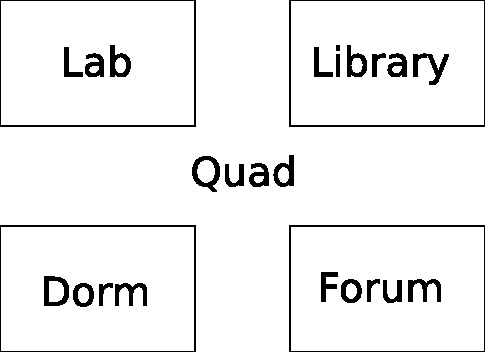
\includegraphics[width=.7\textwidth]{../pictures/PeeragogyEDU.jpg}
\end{center}
\caption*{Map of a virtual campus}
\end{figure}

\begin{figure}
\begin{center}
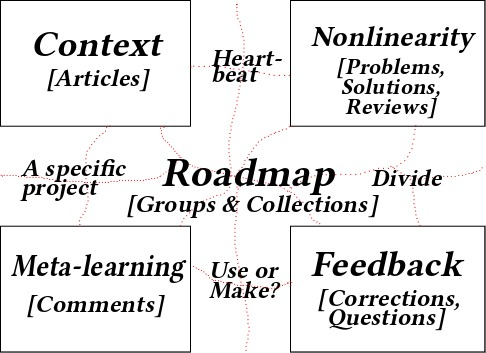
\includegraphics[width=.7\textwidth]{../pictures/PeeragogyEDU-paths.jpg}
\end{center}
\caption*{Peeragogy patterns as loci for ``paths in the grass''}
\end{figure}

\subsection{Initial thematic analysis}

Before describing the new patterns, I will briefly summarize the themes
I identified in the interviews. This can serve as an overview of the
current features and shortcomings of PlanetMath system for people who
are not familiar with it.

\begin{itemize}
\item
  \textbf{``Necessary but not sufficient''.} Users identified a range of
  essential features, like a critical mass of other users to talk to.
\item
  \textbf{``Nice to have''.} It was also easy to identify a bunch of
  cool new ``dream'' features.
\item
  \textbf{Challenges with writing mathematics.} PlanetMath uses LaTeX,
  which isn't entirely easy to learn (however, we could adapt the
  software to help new users get started).
\item
  \textbf{Progressive problem solving.} The new PlanetMath contains
  problems and solutions, but no easy way to talk about conjectures.
  Users would like a better way to share and discuss work-in-progress.
\item
  \textbf{Personal history, social constructivism.} Better features for
  tracking and, where appropriate, sharing, personal history would help
  users make sense of what's happening in the site.
\item
  \textbf{Regulating learning in a social/mediated context.} Different
  users would look for different things to keep them on track (e.g.
  expert guidance, or a due ``sense of urgency'' in feedback from
  peers).
\item
  \textbf{Comparison with roles in other contexts.} Many users expect a
  ``service delivery'' style that is not entirely consistent with the
  ``open'' production model used in a free/open, volunteer-driven
  project. We need to work more on responsiveness in every aspect of the
  project (keeping in mind that most participants are volunteers).
\item
  \textbf{Concreteness as a criterion of quality.} ``Knowing what you
  can do,'' both with the software and with the content, is important.
  On the content level, pictures help.
\item
  \textbf{Personalization and localization.} The system has a
  practically unlimited potential for personalization, although many
  basic personalized interaction modes have not been built yet.
\end{itemize}
\subsection{Pattern analysis}

At the next level of analysis, the themes extracted above were further
analysed in relationship to the peeragogy pattern catalog.

\subsubsection{Frontend and Backend}

Although mathematics is a relatively formal domain, many of the
motivations for using PlanetMath map onto what Zimmerman and Campillo
call informal problem solving {[}3{]}. Informal problems are are
personally defined and possess openended boundary conditions, i.e., are
situated within an ``open world.'' ``Formal'' motivations are are more
likely to be addressed by some variant of a ``look-up'' approach - for
instance, many such problems can be solved by reading the manual. They
do not require the complex, discursive, process of peer supported
problem solving. Acquaintance with the more basic formal features of
mathematical problem solving are typically seen to be a prerequisite for
the more informal activities of mathematics research. This points to the
continued importance of a coherent body of mathematical knowledge in the
form of a well-structured reference resource. This dichotomy suggest a
new and important pattern. This pattern could be called Frontend and
Backend. The ``frontend'' of a system is typically associated with the
formal structural features, while the backend is often associated with
``informal features.'' The Frontend and Backend pattern is related to
the pattern of the ``Newcomer'' pattern, since typically one will not
expect the user of a system to know how to, or to be motivated to, work
with backend features of a system until they have mastered at least some
of the frontend features. It would be rare to find an auto mechanic who
did not know how to drive. David Cavallo wrote about an ``engine
culture'' in rural Thailand, in which structurally open systems made
some of the ``backend'' features of internal combustion engines a part
of daily life {[}4{]}. In PlanetMath, we have an ``open engine'', but
not necessarily an open engine culture (users expect a level of service
provision). The Frontend and Backend pattern clearly lends itself to
standard service provision, but it can also be part of paragogical
activity. For example, sophisticated and committed users of the
PlanetMath website could focus energy on supporting individual
newcomers, by helping them develop a high-quality sub-site on their
topic of interest ({[}RSP8{]}, {[}RSP10{]}). Such effort would
simultaneously inform the development of backend features, and help
raise the profile of the site as a whole. The pattern is in this way
associated with A Specific Project and with the Divide pattern.

\subsubsection{Spanning Set}

You may be able to get what you need without digging - but if you do
need to dig, it would be very good to get some indication about which
direction to dig in. At the content level, this might be achieved by
using high-level ``topic articles'' as a map to the content. But there
is another broader interpretation of this pattern that related to but
distinct from Frontend and Backend - we call this the Spanning Set. In
general, the Spanning Set might be made up of people, or media objects.
In a standard course model, there is one central node, the teacher, who
is responsible for all teaching and course communication. In large
online courses, this model can be is scaled up:

\begin{quote}
\textbf{Anonymous study participant}: {[}E{]}veryone's allocated a
course tutor, who might take on just a half-dozen students - so, they're
not the overall person in charge of the course, by any means.
\end{quote}
Another version is the classical master/apprentice system, in which
every apprentice is supervised by a certified master. In the typical
online Q\&A context, these roles are made distributed, and are better
modeled by power laws than by formal gradations. A ``spanning set'' of
peer tutors could help shift the exponent attached to the power law in
massive courses. We can imagine a given discussion group of 100 persons
that is divided according to the so-called
\href{http://www.wikipatterns.com/display/wikipatterns/90-9-1+Theory}{90/9/1
rule}, so that 90 lurk, 9 contribute a little, and 1 creates the
content. This is what one might observe, for example, in a classroom
with a lecture format. We could potentially shift the system by breaking
the group up, so that each of the 9 contributors leads a small group of
10 persons, at which point, chances are good that some of the former
lurkers would be converted into contributors. At a more semantic level,
we can advance the five paragogical principles and their various
analogues as a candidate description of the fundamental categories and
relationships relevant to peer learning. In practice, principles can
only provide the most visible ``frontend'', and an actual spanning set
is comprised of emergent patterns. In PlanetMath, this would arise from
combining several different features, like a ``start menu'' that shows
what can be done with the site, a Heartbeat built of recurring meetings,
and topic-level guides to content. (Note: as a project with an
encyclopedic component, PlanetMath itself can be used to span and
organize a significantly larger body of existing material.)

\subsubsection{Minimum Viable Project}

The Minimum Viable Product approach to software development is about
putting something out there to see if the customer bites {[}5{]}.
Another approach, related to the pattern we just discussed, is to make
it clear what people can do with what's there and see if they engage. We
might call this the Minimum Viable Project, an adjunct to the
``Roadmap'' pattern, and a new interpretation of the earlier pattern A
Specific Project. One way to strengthen the PlanetMath project as a
whole would be to focus on support for individual projects. The front
page of the website could be redesigned so that the top-level view of
the site is project focused. Thus, instead of collecting all of the
posts from across the site - or even all of the threads from across the
site - the front page could collect succinct summary information on
recently active projects, and list the number of active posts in each,
after the model of Slashdot stories or StackExchange questions. For
instance, each Mathematics Subject Classification could be designated as
a ``sub-project'', but there could be many other cross-cutting or
smaller-scale projects.

\begin{figure}[h]
\begin{center}
\textbf{Frontend and Backend} (\emph{pragma}) \\ Principles and features

\medskip
\textbf{Minimum Viable Project} (\emph{praxis}) \\ A Specific Project,
Roadmap, Heartbeat, Divide, Use or Make

\medskip
\textbf{Spanning Set} (\emph{pratto}) \\ Paths in the grass
\end{center}
\caption*{Paragogical emergent design: a tool for conviviality}
\end{figure}

\subsection{Summary}

This chapter has used the approach suggested by Figure 2 to expand the
peeragogy pattern language. It shows that the peeragogy pattern language
provides a ``meta-model'' that can be used to develop emergent order
relative to given boundary conditions. As new structure forms, this
becomes part of the boundary conditions for future iterations. This
method is a suitable form for a theory of peer learning and peer
production in project-based and cross-project collaborations - a tool
for conviviality in the sense of Ivan Illich. Although this model is
informal, it does suggest one direction for answering the technical
questions posed at the outset of the chapter: in peeragogy, we can
measure learning as a feature of the growth and refinement of the
pattern catalog.


\subsection{References}

\begin{enumerate}
\item
  Gabriel, R. (1996). Patterns of Software. Oxford University Press New
  York.
\item
  Luckin, R. (2010). Re-designing learning contexts: technology-rich,
  learner-centred ecologies. Routledge.
\item
  Zimmerman, B. J. \& Campillo, M. (2003). Motivating self-regulated
  problem solvers. In J. Davidson \& R. Sternberg (Eds.), The psychology
  of problem solving (pp. 233-262). Cambridge University Press New York,
  NY.
\item
  Cavallo, D. P. (2000). Technological Fluency and the Art of Motorcycle
  Maintenance: Emergent design of learning environments (Doctoral
  dissertation, Massachusetts Institute of Technology).
\item
  Ries, E. (2011). The Lean Startup: How today's entrepreneurs use
  continuous innovation to create radically successful businesses. Crown
  Pub.
\end{enumerate}



\part{~Technologies, Services, and Platforms } \label{technologies-part} %%%%%%%%%%%%%%%%%%%%
%
\chapter[\textbf{Peeragogy Technology}]{Introduction to Technologies for Peeragogy}
\attrib{Gigi Johnson}

\textbf{It is tempting to bring a list of technologies out as a glorious
cookbook.} We need a 1/2 cup of group writing tools, 2 tsp. of social
network elements, a thick slice of social bookmarking, and some sugar,
then put it in the oven for 1 hour for 350 degrees.

We have created a broad features/functions list for Handbook readers to
reflect upon and consider. The joy of this list is that you can consider
alternatives for the way you communicate and work while you are planning
the project, or can add in new elements to solve communications gaps or
create new tools.

However, too many tools spoil the broth. In the writing of this
Handbook, we found that out firsthand. We spent a lot of marvelous
energy exploring different tools to collaborate, curate information, do
research, tag resources, and adjudicate among all of our points of view.
In looking at groups working with the various MOOCs, as another example,
different groups of students often camp in different social media
technologies to work.

In large courses, students often have to be pushed into various social
media tools to ``co-create'' with great protest and lots of inertia. And
finally, co-learning groups often come from very different backgrounds,
ages, and stages of life, with very different tools embedded in their
current lives. Do we have time for three more tools in our busy days? Do
more tools help -- or do they interfere with our work?

In this section, we'll share with you a few issues:

\begin{itemize}
\itemsep1pt\parskip0pt\parsep0pt
\item
  What technologies are most useful in peer learning? What do we use
  them for? What features or functions help our co-learning process?
\end{itemize}

\begin{itemize}
\itemsep1pt\parskip0pt\parsep0pt
\item
  How do we decide (a) as a group and (b) for the group on what tools we
  can use? Do we decide upfront, or grow as we go?
\end{itemize}

\begin{itemize}
\itemsep1pt\parskip0pt\parsep0pt
\item
  How do we coach and scaffold each other on use of tools?
\end{itemize}

\begin{itemize}
\itemsep1pt\parskip0pt\parsep0pt
\item
  How much do the tool choices impact the actual outcome of our learning
  project?
\end{itemize}

\begin{itemize}
\itemsep1pt\parskip0pt\parsep0pt
\item
  What are the different roles that co-learners can take in co-teaching
  and co-coaching the technology affordances/assumptions in the project
  to make others' lives easier?
\end{itemize}

Keep in mind -- your needs for tools, plus how the way the group uses
them, will change as the co-learning project moves along.~ Technologies
themselves tend to change rapidly.~ Are you willing to change tools
during the project as your needs and users change, or do you plan to use
a given tool set from the beginning to the end of your project?

\subsection{Features and Considerations}

We will begin below with a discussions of ``features'' and initial
considerations, and then move to a broader ``Choose Your Own
Adventure''-style matrix of features leading to a wide variety of
collaboration-based technology tools online.

\subsubsection{Technologies and Features}

As we will share in the extensive list below, there are abundant tools
now available -- both for free and for pay -- to bring great features to
our co-learning endeavors. It is tempting to grab a group of fancy tools
and bring the group into a fairly complex tool environment to find the
perfect combination of resources. The challenge: adult learners seek
both comfort and context in our lives {[}1{]}, {[}2{]}. In choosing tool
``brands'', we can ignore the features themselves and what we need as
parts of the puzzle for learning. We also can have anxiety about our
self-beliefs around computers and technology, which in turn can limit
our abilities {[}3{]}.

Before we get to brands and choices, it helps to ask a few questions
about the learning goals and environments:

\begin{itemize}
\itemsep1pt\parskip0pt\parsep0pt
\item
  What do we need as features, and at what stage of the learning
  process?
\item
  What are we already comfortable with, individually and as a group?
\item
  Do we want to stay with comfortable existing tools, or do we want to
  stretch, or both?
\item
  What types of learners do we have in this group? Technologically
  advanced? Comfortable with basics?
\item
  Do we want to invest the time to bring the whole group up to speed on
  tools? Do all the group members agree on this? Do we want to risk
  alienating members by making them invest time in new resources?
\item
  We know that our use will migrate and adapt. Do we want to plan for
  adaptation? Observe it? Learn from it? Make that change intentional as
  we go?
\end{itemize}

Researchers over the years have heavily examined these questions of
human, technology, and task fit in many arenas.
\href{http://en.wikipedia.org/wiki/Human-Computer_Interaction}{Human-Computer
Interaction} researchers have looked at ``fit'' and ``adaptive
behavior,'' as well as how the tools can affect how the problem is
presented by Te'eni {[}4{]}. Creativity support tools {[}5{]} have a
whole line of design research, as has the field of
\href{http://en.wikipedia.org/wiki/Computer-supported_cooperative_work}{Computer-Supported
Collaborative Work Systems (CSCW)}. For co-learners and designers
interested in the abundance in this space, we've added some additional
links below. We here will make this a bit easier. For your co-learning
environment, you may want to do one or two exercises in your decision
planning:

What \emph{features do you need}?~ Do you need collaboration? Graphic
models? Places to work at the same time (synchronous)? Between meetings
(asynchronous)? What are the group members \emph{already using} as their
personal learning platforms? It also makes sense to do an inventory
about what the group already has as their learning platforms. I'm doing
that with another learning group right now. People are much more
comfortable -- as we also have found in our co-creation of this Handbook
-- creating and co-learning in tools with which they already are
comfortable. Members can be co-teachers to each other -- as we have have
-- in new platforms. What \emph{type of tools}, based on the features
that we need, shall we start out with?~ Resnick \emph{at al.} {[}6{]}
looked at tools having:

\begin{itemize}
\itemsep1pt\parskip0pt\parsep0pt
\item
  Low thresholds (easy to get people started)
\item
  Wide walls (able to bring in lots of different situations and uses)
  and
\item
  High ceilings (able to do complex tasks as the users and uses adapt
  and grow).
\end{itemize}

What are important features needed for co-creation and \emph{working
together}? In other pages above, we talk abundantly about roles and
co-learning challenges. These issues also are not new; Dourish \&
Bellottii {[}7{]} for example, shared long-standing issues in
computer-supportive collaborative work online about how we are aware of
the information from others, passive vs. active generation of
information about collaborators, etc. These challenges used to be
``solved'' by software designers in individual tools. Now that tools are
open, abundant, and diverse, groups embrace these same challenges when
choosing between online resources for co-learning.

\subsubsection{Useful Uses and fancy Features of Technological Tools}

From here, we will help you think about what might be possible, linking
to features and solution ideas.

We start with ways to ask the key questions: What do you want to do and
why? We will start with features organized around several different
axes:

\begin{enumerate}
\itemsep1pt\parskip0pt\parsep0pt
\item
  Time/Place
\item
  Stages of Activities and Tasks
\item
  Skill Building/Bloom's Taxonomy
\item
  Use Cases, and
\item
  Learning Functions.
\end{enumerate}

Each will link to pages that will prompt you with features,
functionality, and technology tool ideas.

\subsubsection{Time/Place}

We can further break down tools into whether they create or distribute,
or whether we can work simultaneously (synchronous) or at our own times
(ascynchronous). To make elements of time and place more visual, Baecker
{[}8{]} created a CSCW Matrix, bringing together time and place
functions and needs. Some tools are synchronous, such as Google+
Hangouts, Blackboard Collaborate, and Adobe Connect, while others let us
work asynchronously, such as wikis and forums.~ Google Docs can work be
used both ways.~ We seem to be considering here mostly tools good for
group work, but not for solo, while many others are much easier solo or
in smaller groups.

%% \begin{longtable}[c]{@{}lll@{}}
%% \toprule\addlinespace
%% & \textbf{\textbf{Same Time (Synchronous)}} & \textbf{Different Time
%% (Asyncronous)}
%% \\\addlinespace
%% \textbf{Same Place (Co-located)} & \textbf{Face-to Face}:
%% Display-focused (e.g., Smartboards) & \textbf{Continuous Task}:
%% Groupware, project management
%% \\\addlinespace
%% \textbf{Different Place (Remote)} & \textbf{Remote Interaction}:
%% Videoconference, IM, Chat, Virtual Worlds & \textbf{Communication \&
%% Coordination}: Email, bulletin boards, Wikis, blog, workflow tools
%% \\\addlinespace
%% \bottomrule
%% \end{longtable}

Some tools are synchronous, such as Google+ Hangouts, Blackboard
Collaborate, and Adobe Connect, while others let us work asynchronously,
such as wikis, forums, and Google Docs. We seem to be considering here
mostly tools good for group work, but not for solo, while many others
are much easier solo or in smaller groups.

\subsubsection{Stages of Activities and Tasks}

Ben Shneiderman {[}5{]} has simplified the abundant models in this area
(e.g., Couger and Cave) with a clear model of 4 general activities and 8
tasks in creation for individuals, which we can lean on as another
framework for co-creation in co-learning.

%% \begin{longtable}[c]{@{}llll@{}}
%% \toprule\addlinespace
%% \begin{minipage}[t]{0.22\columnwidth}\raggedright
%% \subsection{Collect}
%% \end{minipage} & \begin{minipage}[t]{0.22\columnwidth}\raggedright
%% \subsection{Relate}
%% \end{minipage} & \begin{minipage}[t]{0.22\columnwidth}\raggedright
%% \subsection{Create}
%% \end{minipage} & \begin{minipage}[t]{0.22\columnwidth}\raggedright
%% \subsection{Distribute}
%% \end{minipage}
%% \\\addlinespace
%% \begin{minipage}[t]{0.22\columnwidth}\raggedright
%% Searching Visualizing
%% \end{minipage} & \begin{minipage}[t]{0.22\columnwidth}\raggedright
%% Consulting Others
%% \end{minipage} & \begin{minipage}[t]{0.22\columnwidth}\raggedright
%% Thinking Exploring Composing Reviewing
%% \end{minipage} & \begin{minipage}[t]{0.22\columnwidth}\raggedright
%% Disseminating
%% \end{minipage}
%% \\\addlinespace
%% \bottomrule
%% \end{longtable}

Tools and functions won't be clear cut between areas. For example, some
tools are more focused on being generative, or for creating content.
Wikis, Etherpad, Google docs, and others usually have a commenting/talk
page element, yet generating content is the primary goal and
discursive/consultative functions are in service of that. Some tools are
discursive, or focused on working together for the creative element of
``relating'' above -- Blackboard Collaborate, the social media class
room forums, etc.

\subsubsection{Skill Building (Cognitive, a la Bloom's Taxonomy, see
below)}

Given that we are exploring learning, we can look to Bloom's Taxonomy
(revised, see {[}9{]}) for guidance as to how we can look at knowledge
support. Starting at the bottom, we have:

\begin{itemize}
\itemsep1pt\parskip0pt\parsep0pt
\item
  Remembering, as a base;
\end{itemize}

\begin{itemize}
\itemsep1pt\parskip0pt\parsep0pt
\item
  Understanding,
\end{itemize}

\begin{itemize}
\itemsep1pt\parskip0pt\parsep0pt
\item
  Applying,
\end{itemize}

\begin{itemize}
\itemsep1pt\parskip0pt\parsep0pt
\item
  Analyzing,
\end{itemize}

\begin{itemize}
\itemsep1pt\parskip0pt\parsep0pt
\item
  Evaluating, and then, at the top,
\end{itemize}

\begin{itemize}
\itemsep1pt\parskip0pt\parsep0pt
\item
  Creating.
\end{itemize}

We could put ``search'' in the Remembering category above. Others
contest that Search, done well, embraces most of the Bloom's elements
above. Samantha Penney has created a
\href{http://www.usi.edu/distance/bdt.htm}{Bloom's Digital Taxonomy
Pyramid} infographic, describing tools for learning, which you may want
to check out.

\subsubsection{Use Cases (I want to\ldots{}.)}

Technologies can be outlined according to the need they serve or use
case they fulfill. Examples: If we need to `curate', Pearl Trees is an
option. To `publish' or `create', we can look to a wiki or wordpress.
Other choices might be great in order to `collaborate', etc.

One challenge is that tools are not that simple. As we look more closely
at the technologies today, we need to reach more broadly to add multiple
tags to them. For example Twitter can be used for ``Convening a group,''
for ``micro-blogging,'' for ``research,'' etc.

\begin{itemize}
\itemsep1pt\parskip0pt\parsep0pt
\item
  Collaborate with a Group
\item
  Create Community
\item
  Curate Information 
\item
  Research
\item
  Publish Information
\item
  Create Learning Activities
\item
  Make Something
\end{itemize}

These plans get more complex, as you are making a group of decisions
about tool functionality in order to choose what combination works for
use cases. It may be most useful to use a concept map (a tech tool) to
think about the needs and combinations that you would bring together to
achieve each Use Case or Learning Module.

\subsubsection{Technology Features/Functions}

We have not made this easy! There are lots of moving elements and
options here, none of them right for everything, and some of them
fabulous for specific functions and needs. Some have the low thresholds
but may not be broad in scope. Some are broad for many uses; others are
specific task-oriented tools. That is some of the charm and frustration.

Weaving all of the above together, we have brought together a shared
taxonomy for us to discuss and think about co-learning technology
features and functions, which we present as an appendix below. This
connects various technology features within an expanded version of Ben
Shneiderman's creativity support tools framework. We've created this
linked toolset with multiple tags, hopefully making it easier for you to
evaluate which tool suits best the necessities of the group. Please
consider this a starting point for your own connected exploration.

\subsection{Appendix: Features and Functions}

Weaving all of these frameworks together, we have brought together a
shared taxonomy for us to discuss and think about co-learning technology
features and functions. We have connected various technology features
with an expanded version of Ben Shneiderman's creativity support tools
framework for the linked resource guide.~ For convenience and to help
keep it up to date, we're publishing this resource
\href{http://goo.gl/H02fMA}{on Google Docs}.~~ We present an overview
below.

%% \begin{longtable}[c]{@{}ll@{}}
%% \toprule\addlinespace
%% \begin{minipage}[t]{0.47\columnwidth}\raggedright
%% \subsection{Activities \& Tasks}
%% \end{minipage} & \begin{minipage}[t]{0.47\columnwidth}\raggedright
%% \subsection{Features/Functions}
%% \end{minipage}
%% \\\addlinespace
%% \begin{minipage}[t]{0.47\columnwidth}\raggedright
%% \textbf{Planning/Designing}

%% \begin{itemize}
%% \itemsep1pt\parskip0pt\parsep0pt
%% \item
%%   Communicating
%% \item
%%   Deciding and Creating Alternatives
%% \end{itemize}
%% \end{minipage} & \begin{minipage}[t]{0.47\columnwidth}\raggedright
%% \begin{itemize}
%% \itemsep1pt\parskip0pt\parsep0pt
%% \item
%%   Convening a group
%% \item
%%   Planning a course/structure (assembling a syllabus, designing a
%%   learning activity)
%% \item
%%   Designing self-assessment (group and individual)
%% \item
%%   Setting individual and group goals
%% \item
%%   Brainstorming
%% \item
%%   Visualizing
%% \end{itemize}
%% \end{minipage}
%% \\\addlinespace
%% \begin{minipage}[t]{0.47\columnwidth}\raggedright
%% \textbf{Collect/Share}

%% \begin{itemize}
%% \itemsep1pt\parskip0pt\parsep0pt
%% \item
%%   Searching
%% \item
%%   Visualizing
%% \end{itemize}
%% \end{minipage} & \begin{minipage}[t]{0.47\columnwidth}\raggedright
%% \begin{itemize}
%% \itemsep1pt\parskip0pt\parsep0pt
%% \item
%%   Search
%% \item
%%   Social Bookmarking
%% \item
%%   Creating/Finding Taxonomies (shared keywords, domain-based keywords)
%% \item
%%   Programming Toolsets
%% \item
%%   Collaborative reading
%% \item
%%   Collaborative note-taking
%% \item
%%   Curation Tools
%% \item
%%   Gathering information (e.g., capturing audio, video, text)
%% \item
%%   Surveys and Questionnaires
%% \end{itemize}
%% \end{minipage}
%% \\\addlinespace
%% \begin{minipage}[t]{0.47\columnwidth}\raggedright
%% \textbf{Relate}

%% \begin{itemize}
%% \itemsep1pt\parskip0pt\parsep0pt
%% \item
%%   Consulting Others from the Outside
%% \end{itemize}
%% \end{minipage} & \begin{minipage}[t]{0.47\columnwidth}\raggedright
%% \begin{itemize}
%% \itemsep1pt\parskip0pt\parsep0pt
%% \item
%%   Qualitative research
%% \item
%%   Quantitative research
%% \end{itemize}
%% \end{minipage}
%% \\\addlinespace
%% \begin{minipage}[t]{0.47\columnwidth}\raggedright
%% \textbf{Communication}

%% \begin{itemize}
%% \itemsep1pt\parskip0pt\parsep0pt
%% \item
%%   Connecting with Others in the Group
%% \end{itemize}
%% \end{minipage} & \begin{minipage}[t]{0.47\columnwidth}\raggedright
%% \begin{itemize}
%% \itemsep1pt\parskip0pt\parsep0pt
%% \item
%%   Project Planning - Scheduling
%% \item
%%   Voice/Video Conferencing Services
%% \item
%%   Group Email / Forum Messaging Services
%% \item
%%   File Sharing Service (cloud based)
%% \item
%%   Screen Capturing and Screen Casting
%% \item
%%   Presentation and Document Sharing
%% \end{itemize}
%% \end{minipage}
%% \\\addlinespace
%% \begin{minipage}[t]{0.47\columnwidth}\raggedright
%% \textbf{Co-Create}

%% \begin{itemize}
%% \itemsep1pt\parskip0pt\parsep0pt
%% \item
%%   Thinking (Free Association)
%% \item
%%   Exploring
%% \item
%%   Composing
%% \item
%%   Reviewing
%% \end{itemize}
%% \end{minipage} & \begin{minipage}[t]{0.47\columnwidth}\raggedright
%% \begin{itemize}
%% \itemsep1pt\parskip0pt\parsep0pt
%% \item
%%   Learning Management Systems
%% \item
%%   Document Collaboration and Editing
%% \item
%%   Visualizing Information for analysis and synthesis (concept maps, data
%%   visualization)
%% \end{itemize}
%% \end{minipage}
%% \\\addlinespace
%% \begin{minipage}[t]{0.47\columnwidth}\raggedright
%% \textbf{Distribute/Action}

%% \begin{itemize}
%% \itemsep1pt\parskip0pt\parsep0pt
%% \item
%%   Disseminating
%% \end{itemize}
%% \end{minipage} & \begin{minipage}[t]{0.47\columnwidth}\raggedright
%% \begin{itemize}
%% \itemsep1pt\parskip0pt\parsep0pt
%% \item
%%   Publishing Platforms (traditional publishing, social media/sharing
%%   distribution)
%% \item
%%   Visualization (for presentation)
%% \end{itemize}
%% \end{minipage}
%% \\\addlinespace
%% \begin{minipage}[t]{0.47\columnwidth}\raggedright
%% \textbf{Feedback}

%% \begin{itemize}
%% \itemsep1pt\parskip0pt\parsep0pt
%% \item
%%   Listening
%% \end{itemize}
%% \end{minipage} & \begin{minipage}[t]{0.47\columnwidth}\raggedright
%% \begin{itemize}
%% \itemsep1pt\parskip0pt\parsep0pt
%% \item
%%   Social Monitoring
%% \end{itemize}
%% \end{minipage}
%% \\\addlinespace
%% \bottomrule
%% \end{longtable}

\subsubsection{References}

\begin{enumerate}
\itemsep1pt\parskip0pt\parsep0pt
\item
  Schein, E. H. (1997). \emph{Organizational learning as cognitive
  re-definition: Coercive persuasion revisited}. Cambridge, MA: Society
  for Organizational Learning.
\item
  Schein, E. H. (2004). \emph{Organizational culture and leadership.}
  San Francisco, CA: Jossey-Bass.
\item
  Compeau, D.R., \& Higgins, C.A. (1995, June). Computer Self-Efficacy:
  Development of a Measure and Initial Test. \emph{MIS Quarterly, 19},
  (2), 189-211.
\item
  Te'eni, D. (2006). Designs that fit: An overview of fit
  conceptualizations in HCI. In \emph{Human-Computer Interaction and
  Management Information Systems: Foundations}, edited by P. Zhang and
  D. Galletta, pp. 205-221, Armonk, NY: M.E. Sharpe.
\item
  Shneiderman, B. (2002). Creativity support tools. \emph{Commun. ACM}
  45, 10 (October 2002), 116-120.
\item
  Resnick, M, Myers, B, Nakakoji, K, Shneiderman, B, Pausch, R, Selker,
  T. \& Eisenberg, M (2005).
  \href{http://repository.cmu.edu/isr/816}{Design principles for tools
  to support creative thinking}. \emph{Institute for Software Research.}
  Paper 816.
\item
  Dourish, P. \& Bellotti, V. (1992). Awareness and coordination in
  shared workspaces. In \emph{Proceedings of the 1992 ACM conference on
  Computer-supported cooperative work} (CSCW '92). ACM, New York, NY,
  USA, 107-114.
\item
  Baecker, R., \href{http://www.interaction-design.org/references/authors/jonathan_grudin.html}{Grudin},
  J.,
\href{http://www.interaction-design.org/references/authors/william_buxton.html}{Buxton},
  W., \&
\href{http://www.interaction-design.org/references/authors/saul_greenberg.html}{Greenberg}, \& (eds.) (1995): \emph{Readings in Human-Computer Interaction: Toward
  the Year 2000.} New York, NY: Morgan Kaufmann Publishers
\item
  Anderson, L. W., \& Krathwohl, D. R. (Eds.). (2001). \emph{A taxonomy
  for learning, teaching and assessing: A revision of Bloom's Taxonomy
  of educational objectives: Complete edition}. New York, NY: Longman.
\end{enumerate}

%
\chapter[\textbf{Forums}]{ Forums } 
%
\attrib{Howard Rheingold}

\begin{quote}
Forums are web-based communication media that enable groups of people to
conduct organized multimedia discussions about multiple topics over a
period of time. Selecting the right kind of platform for forum
conversations is important, as is know-how about facilitating ongoing
conversations online. Forums can be a powerful co-learning tool for
people who may have never met face-to-face and could be located in
different time zones, but who share an interest in co-learning.
Asynchronous media such as forums (or simple email distribution lists or
\href{http://www.youtube.com/watch?v=VVFbqHhkb-k}{Google Docs}) can be
an important part of a co-learning toolkit that also include synchronous
media from face-to-face meetups to
\href{http://www.google.com/+/learnmore/hangouts/}{Google+ Hangouts} or
webinars via
\href{http://www.blackboard.com/Platforms/Collaborate/Products/Blackboard-Collaborate.aspx}{Blackboard
Collaborate},
\href{http://www.adobe.com/products/adobeconnect.html}{Adobe Connect},
or the open source webconferencing tool,
\href{http://www.bigbluebutton.org/}{Big Blue Button}).
\end{quote}

\subsubsection{What is a forum and why should a group use it?}

A forum, also known as a message board,
\href{http://en.wikipedia.org/wiki/Bulletin_board_system}{bbs}, threaded
discussion, or conferencing system, affords asynchronous, many-to-many,
multimedia discussions for large groups of people over a period of time.
That means that people can read and write their parts of the discussion
on their own schedule, that everyone in a group can communicate with
everyone else, and that graphics, sounds, and videos can accompany text.
The best forums index discussion threads by topic, title, tag,
date,and/or author and also keep track of which threads and entries
(also known as posts) each logged-in participant has already read,
making it possible to click on a ``show me all the new posts and
threads'' link each time a participant logs in. This particular form of
conversational medium meets the need for organizing conversations after
they reach a certain level of complexity. For example, if twenty people
want to discuss five subjects over ten days, and each person makes one
comment on each subject every day, that makes for one thousand messages
in each participant's mailbox. On email lists, when the conversation
drifts from the original topic, the subject line usually does not
change, so it makes it difficult to find particular discussions later.

Forums make possible a new kind of group discussion that unfolds over
days, weeks, and months, in a variety of media. While blogs are
primarily about individual voice, forms can be seen as the voice of a
group. The best forum threads are not serial collections of individual
essays, but constitute a kind of discourse where the discussion becomes
more than the sum of its individual posts. Each participant takes into
account what others have said, builds on previous posts, poses and
answers questions of others, summarize, distill, and concludes.

This short piece on
\href{http://www.lehigh.edu/~indiscus/doc_guidelines.html}{guidelines
for discussion board writing}is useful, as is this short piece on
\href{http://academiccommons.org/commons/essay/shaping-culture-conversation}{shaping
a culture of conversation}. Lively forums with substantial conversation
can glue together the disparate parts of a peeragogy group -- the
sometimes geographically dispersed participants, texts, synchronous
chats, blogs, wikis and other co-learning tools and elements. Forum
conversations are an art in themselves and forums for learning
communities are a specific genre. Reading the resources linked here --
and communicating about them -- can help any peeragogy group get its
forums off to a good start

\subsubsection{How to start fruitful forum discussions:}

In most contexts, starting a forum with a topic thread for introductions
tends to foster the sense of community needed for valuable
conversations.
\href{http://www.rheingold.com/texts/artonlinehost.html}{This short
piece on how to host good conversations online}offers general advice. In
addition to introductions, it is often helpful to start a topic thread
about which new topic threads to create -- when everybody has the power
to start a new thread and not everybody knows how forums work, a
confusing duplication of conversations can result, so it can be most
useful to make the selection of new topic threads a group exercise. A
topic thread to ask questions about how to use the forum can prevent a
proliferation of duplicate questions. It helps to begin a forum with a
few topic threads that invite participation in the context of the
group's shared interest ``Who is your favorite photographer'' for a
group of photographers, for example, or ``evolution of human
intelligence'' for a group interested in evolution and/or human
intelligence. Ask questions, invite candidate responses to a challenge,
make a provocative statement and ask for reactions.

Whether or not you use a rubric for assessing individual participants'
forum posts, this guide to
\href{http://www.wpi.edu/Academics/ATC/Collaboratory/Idea/boards.html}{how
forum posts are evaluated} by one professor can help convey the
difference between a good and a poor forum conversation:

\emph{4 Points -}The posting(s) integrates multiple viewpoints and
weaves both class readings and other participants' postings into their
discussion of the subject.

\emph{3 Points -}The posting(s) builds upon the ideas of another
participant or two, and digs deeper into the question(s) posed by the
instructor.

\emph{2 Points -}A single posting that does not interact with or
incorporate the ideas of other participants' comments.

\emph{1 Point -}A simple ``me too'' comment that neither expands the
conversation nor demonstrates any degree of reflection by the student.

\emph{0 Points -}No comment.

\subsubsection{Selecting a forum platform}

\begin{itemize}
\itemsep1pt\parskip0pt\parsep0pt
\item
  You don't want a forum for discussions among two or three people; you
  do want a forum for discussions among half a dozen or five thousand
  people.
\item
  You don't want a forum for exchanges of short duration (an hour, a day
  or two) among any number of people; you do want a forum for ongoing
  conversations that can continue for months.
\item
  You don't want a forum if blogs with comment threads will do -- blogs
  with comments afford group discourse, but is not easily indexed and
  discourse gets complicated with more than a dozen or so bloggers and
  commenters.
\end{itemize}

If you do want to select a platform for forum discourse, you will want
to decide whether you have the technical expertise available to install
the software on your own server or whether you want to look for a hosted
solution. Cost is an issue.

Fortunately, an online forum maven by the name of
\href{http://thinkofit.com/whoweare.htm}{David Wooley} has been keeping
an up-to-date list of available software and services for more than a
decade:

\begin{itemize}
\itemsep1pt\parskip0pt\parsep0pt
\item
  \href{http://thinkofit.com/webconf/forumsoft.htm}{Forum Software for
  the Web}
\item
  \href{http://thinkofit.com/webconf/hostsites.htm}{Forum and Message
  Board Hosting Services}
\end{itemize}

These
\href{https://docs.google.com/document/d/1D606u7SfVD3p7xH0lbf2mOO1hIdX97r7kVe753hSYeE/edit}{2003
suggestions on how to choose a forum} by Howard Rheingold can be
helpful. If blogs with comments afford a kind of networked
individualistic discourse, and video conferencing emulates face-to-face
meeting, forums can be seen as a channel for expression of the group
voice. When people react to and build on each other's comments, they can
learn to act as a collective intelligence as well as a collection of
individuals who are communicating in order to learn.

~

%
\chapter[\textbf{Wiki}]{ Wiki } 
%
\emph{Author:} Régis Barondeau \\

In the context of P2P-learning, a wiki platform can be a useful and
powerful collaboration tool. This section will help you understand what
a wiki is and what it is not, why you should use it, how to choose a
wiki engine and finally how you could use it in a P2P context. Some
examples of P2P-learning projects run on wikis will help you see the
potential of the tool.

\subsection{What is a wiki?}

For \href{http://en.wikipedia.org/wiki/Ward\_cunningham}{Ward
Cunningham} father of the wiki, ``a wiki is a freely expandable
collection of interlinked Web `pages', a hypertext system for storing
and modifying information - a database, where each page is easily
editable by any user with a forms-capable Web browser client'' {[}1{]}.

According to Wikipedia : ``a wiki is a website whose users can add,
modify, or delete its content via a web browser using a simplified
markup language or a rich-text editor'' {[}2{]}.

You can watch this CommonCraft video
\href{http://www.youtube.com/watch?v=-dnL00TdmLY}{wiki in plain english}
to better understand what a wiki is.

\subsection{What differentiates the wiki from other co-editing tools?}

The previous definitions show that a wiki is a ``website,'' in other
words it is composed of pages that are connected together by
hyperlinks.In additiont every authorized person (not all wikis are
totally open like Wikipedia) can edit the pages from a web browser,
reducing time and space constrains. In case one saves a mistake or for
any other reason would like to go back to a previous version, a feature
called ``history'' allows users to see previous versions and to roll
back any of them. This version history allows also to compare versions
avoiding the cluttered of the ``commentaries rainbow'' we are used too
in popular Word processors. For example if you work on a wiki page, and
come back later on, you will be able to catch up by comparing your last
version with the lastest version of someone else.

Tools like \href{https://docs.google.com/}{Google Docs} or
\href{http://en.wikipedia.org/wiki/Etherpad}{Etherpad} are design to
enable co-editing on a single document. This can be seen as a ``wiki
way'' of working on a document as it is web based and includes
versioning. But it is not a wiki because a single document is not a
website. Those tools offer realtime collaboration which wikis do not and
are so far easier to use for beginners as they work in
\href{http://en.wikipedia.org/wiki/WYSIWYG}{WYSIWYG} mode, which many
wikis do not support. However, the advanced features
\href{http://en.wikipedia.org/wiki/Wiki\_syntax}{wiki markup language}
make it a more powerful tool. In summary, tools like Googles Docs or
Etherpad are a great way to quickly collaborate (synchronously,
asynchronously, or a mixture of both) on a single document for free,
with a low barrier to entry and no technical support. (Note that
Etherpad does have a ``wiki-links'' plugin that can allow it to be used
in a more wiki-like way; \href{https://hackpad.com/}{Hackpad} is another
real-time editing tool that prominently features linking -- and it
claims to be ``the best wiki ever''.)

Using a real wiki engine is more interesting for bigger projects and
allows a huge number of users to collaborate on the same platform. A
wiki reduces the coordination complication as e-mails exchanges are no
more needed to coordinate a project. On the other hand it can help us
deal with complexity ({[}3{]}, {[}4{]}) especially if you put basic simple
rules in place like the Wikipedia's
\href{http://en.wikipedia.org/wiki/NPOV}{neutral point of view} to allow
every participant to share her or his ideas.

Going back to the continuum we talked about before, some tools like
Moodle, SharePoint, WordPress, Drupal or others have build in wiki
features. Those features can be good but will typically not be as good
for wiki-building purposes as a well-developed special-purpose wiki
engine. In other words, those tools main focus is not the wiki, which is
only a secondary feature. When you choose a real wiki engine like
\href{http://www.mediawiki.org/}{Mediawiki},
\href{http://www.tiki.org/}{Tiki}, \href{http://foswiki.org/}{Foswiki},
etc., the wiki will be your platform, not a feature of it. For example
if you start a wiki activity in a Moodle course, this wiki will be only
visible to a specific group of students and searchable only to those
students. On the other hand if your learning platform is a wiki, the
whole platform will be searchable to all members regarding their
permissions. We are not saying here that a wiki is better than other
tools but if you need a wiki engine to address your needs you may
consider going with a strong wiki engine rather than a ``micro-wiki''
engine embedded in an other tool.

\subsection{Why use a wiki?}

Those are the main reasons you should consider a wiki for your peer
learning projects :

\begin{itemize}
\item
  To reduce coordination complication by having a central and always up
  to date place to store your content. You will reduce e-mail usage
  drasticly, and have access to your content from everywhere using any
  operating system.
\item
  To keep track of the evolution of your project and be able to view or
  roll back any previous version of a wiki page using the history
  feature.
\item
  To make links between wiki pages to connect ideas and people but also
  make links to external URL's. This last possibility is very handy to
  cite your sources.
\item
  To deal with complexity. As a wiki allows anyone to contribute, if you
  set some easy rules like Wikipedia's NPOV (Neutral Point of View), you
  will be able to catch more complexity as you will allow everyone to
  express his or her opinion. Wikis also integrate a forum or comment
  feature that will help you solve editing conflicts.
\item
  To deal with work in progress. A wiki is a great tool to capture an on
  going work.
\item
  To support transparency by letting every members of the community see
  what others are doing.
\item
  To support a network structure as a wiki is by essence an horizontal
  tool. 
\end{itemize}

Using hyperlinks, you can\ldots{}

\begin{quote}
\textbf{Gérard Ayache}: ``\ldots{}jump by a single
  click from one network node to another, from a computer to another,
  from one piece of information to another, from one universe to
  another, from one brain to another.'' (Translated from {[}5{]}.)
\end{quote}

\subsection{How to choose a wiki engine?}

You will find more than a hundred different wiki engines. 

The first main
distinction is between open source ones that are free to download and
commercial ones you will have to pay for. You will find powerful engines
on both sides open source and commercial. Sometimes the open source ones
look less polished at first sight but are backed by a strong community
and offer a lot of customization possibilities. The commercial are sold
like a package, they are nicely presented but often they offer less
customization on the user side and additional feature or custom made
tools will cost you an extra fee. 

The second distinction that we can
make is between wiki farms and self-hosted wikis. The
\href{http://en.wikipedia.org/wiki/Wiki\_hosting\_service}{wiki farm} is
a hosting service you can find for both open source or commercial wikis.
The goal of those farms is to simplify the hosting of individual wikis.
If you don't want to choose a wiki farm hosting, you will have to host
the wiki on your own server. This will give you more latitude and data
privacy but will require more technical skills and cost you maintenance
fees.

The \href{http://www.wikimatrix.org/}{Wikimatrix} web site will help you
choose the best wiki for your needs. It allows you to compare the
features of more than a hundred wiki engines.
\href{http://c2.com/cgi/wiki?TopTenWikiEngines}{Here} is the top ten
list of the best wiki engines by Ward Cunningham.

\subsection{How can a wiki be useful in a peeragogy project?}

A wiki is a good tool collaborative projects and a specially suited for
work in progress as you can easily track changes using the history,
compare those version and if necessary roll back a previous versions. In
other words, nothing gets lost.

Here are some ideas about how to use a wiki in a peeragogy project :

\begin{itemize}
\item
  \textbf{Use a wiki as your learning platform}. It can also support
  \href{http://socialmediaclassroom.com/host/peeragogy/wiki/connectivism-practice-how-organize-a-mooc}{Massive
  Open Online Courses (MOOCs)}. A wiki will help you organize your
  \href{http://socialmediaclassroom.com/host/peeragogy/wiki/organizing-a-learning-context}{learning
  context}. You can choose to give access to your wiki only to the
  project participants or open it to the public like
  \href{http://www.wikipedia.org/}{Wikipedia}. Using hyperlinking, you
  will operationalize the theory of
  \href{http://en.wikipedia.org/wiki/Connectivism}{connectivism} by
  connecting nodes together. As a learning platform wikis are powerful
  because you can easily see what others are doing, share with them, get
  inspired, merge ideas or link to ideas. In other words, it creates
  emulation between learners. For additional ressources about wiki in
  education follow this Diigo
  \href{http://www.diigo.com/user/regisb/wiki\%20education}{link}.
\end{itemize}
\begin{itemize}
\item
  \textbf{Manage your peeragogy project}. A wiki is an excellent tool
  for project collaboration. Above all, the wiki can be a central place
  for peer learners to write or link to content. Even if you use several
  technologies to run your project as we did to write this handbook, at
  the end of the day, all the content can be centralized on a wiki using
  direct writing on wiki pages or hyperlinks. This way members can
  access the content from anywhere and from any device connected to the
  internet using any platform or application and they will always see
  the most recent version while being able to browse through the
  versions history to understand what has changed since their last
  visit.
\end{itemize}
\begin{itemize}
\item
  \textbf{Publish your project}. As a wiki is a website you can easily
  use it to show your work to the world. Regarding web design, don't
  forget that a wiki can look way better than a Wikipedia page if you
  customize it
\end{itemize}
\subsection{Examples of peeragogy projects run on wikis}

\href{http://www.appropedia.org/Welcome\_to\_Appropedia}{Appropedia} is
a wiki site for collaborative solutions in
\href{http://www.appropedia.org/Sustainability}{sustainability},
\href{http://www.appropedia.org/Poverty}{poverty} reduction and
\href{http://www.appropedia.org/International\_development}{international
development} through the use of sound
\href{http://www.appropedia.org/Principles}{principles} and
\href{http://www.appropedia.org/Appropriate\_technology}{appropriate
technology} and the sharing of wisdom and
\href{http://www.appropedia.org/Project}{project} information. The site
is open to stakeholders to find, create and improve scalable and
adaptable solutions.

\href{http://en.wikipedia.org/wiki/Wikipedia:Teahouse}{Teahouse} is a
peeragogy project run on a wiki that gives newcomers a place to learn
about Wikipedia culture and get feedback from experienced Wikipedians.

\subsection{What are the best practices when using a wiki?}

\begin{itemize}
\item
  \textbf{Cofacilitation} -- help each other learn, help each other
  administer
\item
  \textbf{Self-election} -- enable people to choose what they want to
  work on, at their own pace, in their own way
\item
  \textbf{Communication} -- use comment threads and talk pages to
  discuss wiki changes
\item
  \textbf{Documenting changes} -- most wikis enable editors to write
  very brief descriptions of their edits
\item
  \textbf{Rules} -- keep rules at a minimum level to avoid chaos without
  constraining creativity
\item
  \textbf{Fun} -- make it fun for people to contribute
\end{itemize}
\subsection{References}

\begin{enumerate}
\item
  Leuf, Bo, et Ward, Cunningham. 2001. The Wiki way : quick
  collaboration on the Web. Boston: Addison-Wesley, xxiii, 435 p. p.14
\item
  \href{http://en.wikipedia.org/wiki/Wiki}{Wiki} on Wikipedia
\item
  Andrus, Calvin D. 2005. \href{http://ssrn.com/abstract=755904}{Toward
  a complex adaptative intelligence community - The wiki and the blog}.
  Studies in Intelligence. vol. 49, no 3. Online :
\item
  Barondeau, Régis. 2010.
  \href{http://www.regisbarondeau.com/Chapitre+4\%3A+Analyse+du+cas\#Synth\_se}{La
  gestion de projet croise le wiki}. École des Sciences de la Gestion,
  Université du Québec à Montréal, 180 pp.
\item
  Ayache, Gérard. 2008. Homo sapiens 2.0 : introduction à une histoire
  naturelle de l'hyperinformation. Paris: Milo, 284 p. p.179
\end{enumerate}

%
\chapter[\textbf{Real-time Meetings}]{ Real-time Meetings } 
%
\attrib{Howard Rheingold}
%
\begin{quote}
Web services that enable broadband-connected learners to communicate
in real time via audio, video, slides, whiteboards, chat, and
screen-sharing enable learning groups to add some of the audio-visual
dimensions familiar from synchronous face-to-face communication to
otherwise asynchronous platforms such as forums, blogs, and
wikis. This article includes resources for finding and evaluating
appropriate for-free or for-fee platforms, tips on participative
activities for real-time meetings, and suggestions for blending
real-time and asynchronous media.
\end{quote}

\subsection{Real-time meeting media}

The \emph{Peeragogy Handbook} was conceived and constructed by a group
of people on four continents who had not met and had not known about
each other before we began meeting online. The process involves
asynchronous media, including forums, wikis, social bookmarking groups,
and Wordpress, but it probably would never have cohered into a group
capable of collective action if it had not been for the real-time
meetings where we were able to see each other's faces, hear each other's
voices, use a whiteboard as an anonymous agenda-generator, exchange
links in chat, show each other examples through screen-sharing.
Together, the asynchronous and real-time media enabled us to begin to
see ourselves as an effective group. We used both real-time and
asynchronous tools to work out processes for creating, refining, and
publishing the Handbook, to divide labor, decide on platforms and
processes, to collaboratively compose and edit articles, and to design
and add graphical and video elements. In particular, we used the
\href{http://www.blackboard.com/platforms/collaborate/overview.aspx}{Blackboard
Collaborate} platform, a web-service that enables up to 50 people at a
time to meet in a multimedia, recordable, meeting room for around
\$500/year. We've experimented with other paid platforms, such as
\href{http://success.adobe.com/en/na/sem/products/connect/1109_6011_connect_webinars.html}{Adobe
Connect} (about the same price as Collaborate), and when we meet in
groups of ten or less, we often use the free and recordable
\href{http://www.google.com/+/learnmore/hangouts/}{Google+ Hangout}
service. Smaller groups also use \href{http://www.skype.com}{Skype} or
free telephone conferencing
services.~~\href{http://mumble.sourceforge.net/}{Mumble} is an open
source audio-only tool that is popular with gamers. We're watching the
development of \href{http://www.bigbluebutton.org/}{Big Blue Button}, a
free and open-source real-time meeting platform, as it develops the full
suite of tools that are currently only available for a fee. Dozens of
other free, ad-supported and/or freemium webconferencing systems such as
\href{http://www.bigmarker.com/about}{Big Marker} and
\href{http://www.dimdim.com}{Dim-Dim} can be found in lists like
\href{http://delicious.com/hrheingold/webconferencing}{Howard
Rheingold's} and~\href{http://www.mindmeister.com/12213323/best-online-collaboration-tools-2012-robin-good-s-collaborative-map}{Robin
Good's} (see links at the end of this chapter). Free phone conferencing services provide another technological
``lowest common denominator'': some provide a few extras like
downloadable recordings.

{\centering
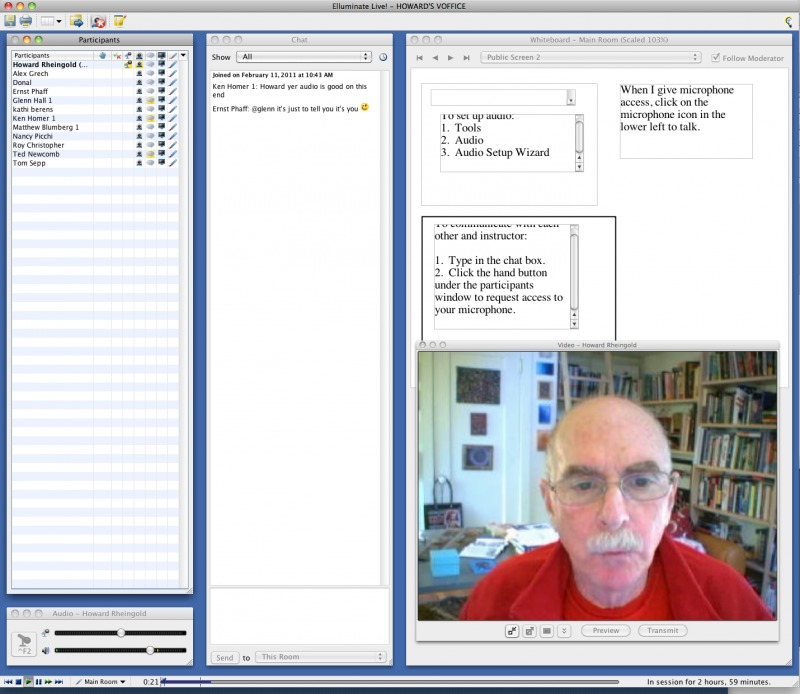
\includegraphics[width=.9\textwidth]{../pictures/elluminate.jpg}
\par}

\subsection{Features of real-time meeting platforms}

There are many free services for chat, screen-sharing, whiteboards, and
video conferencing, but combining all these components in separate panes
of the same screen (preferably) or as separate tabs of a browser can
have a powerful synchronizing and harmonizing effect on the group. The
features to look for in meeting platforms include:

\textbf{Audio and video}: Choose platforms that enable
voice-over-internet-protocol (VOIP) and easy ways for participants to
configure their microphones and speakers. Today's webcams, together with
adequate lighting and a broadband connection, enable a number of people
to be visible at the same time. In Blackboard Collaborate, the person
who is speaking at a given moment is visible in the largest video pane,
while other participants are available in smaller video windows. Audio
and video convey much more of a human dimension than text communications
alone. A group of people who have seen and heard each other online are
able to work together via asynchronous media such as forums and wikis
more effectively. Online face-to-face meetings are often the best way
for a group to argue constructively and decide on critical issues.
Forums and email are comparatively bad choices for distributed
decison-making.

\textbf{Slide pushing:} The best platforms will convert .ppt or .pdf
files for sequential display. With the addition of text chat,
annotations to slides, and the ability to ``raise your hand'' or
interrupt with your voice, an online lecture can be a more
multidimensional experience than even a highly discursive in-person
lecture.

\textbf{Text chat:} As a backchannel, a means of quickly exchanging
links to relevant resources, a channel for collaborative note-taking, a
way of communicating with the lecturer and with other participants, text
chat adds a particularly useful dimension to real-time peeragogical
meetings -- especially when the division of labor is explicitly agreed
upon in advance. We've found that even in meetings that use the
real-time collaborative editor \href{http://etherpad.org}{Etherpad} for
collaborative note taking, participants may gravitate toward the
built-in chat box for discussion.

\textbf{Screen sharing:} The ability of participants to show each other
what is on their screens becomes especially important in peer learning,
where we all have some things to show each other.

\textbf{Web tours:} An alternative to screen-sharing is the ability to
display the same web page(s) to all participants by entering URLs.

\textbf{Interactive whiteboards}: A shared space that enables
participants to enter text, drawings, shapes, colors, to move and resize
media, and to import graphic content -- especially if it allows
anonymous actions -- can foster the feeling of participating in a
collective intelligence. Collaborative anonymous mind-mapping of the
discussion is one technique to try with whiteboards. The whiteboard can
also be used to generate an emergent agenda for an ``un-meeting''.

\subsection{Configuring Google+ Hangout - a free alternative for up to
10 people}

For up to 10 people, each equipped with a webcam, microphone, and
broadband connection,
\href{http://lifehacker.com/5842191/google\%252B-hangouts-adds-screen-sharing-google-docs-collaboration-and-more}{Google+
Hangout} can provide high-quality audio-video conferencing. By enabling
the text-chat feature and adding Google Docs (text documents,
presentations, or spreadsheets), screensharing, and SketchUp
(whiteboard), it is possible to emulate most of what the commercial
services offer.~ Adobe Connect and Blackboard Collaborate currently have
the user-interface advantage of displaying chat, video,
whiteboard/slides as resizable panes on one screen; at present, the free
Google services can provide a powerful extension of the basic
audio-video platform, but participants have to shift between different
tabs or windows in the browser. Note that it is possible to
\href{http://www.google.com/+/learnmore/hangouts/onair.html}{stream a
Hangout and record it to YouTube}, again at no cost to the user.~ We've
used this tool extensively in the Peeragogy project.

\subsection{Suggestions for real-time meetings}

In the nine online courses I have facilitated, the emphasis on
co-learning encouraged participants to suggest and shape active roles
during real-time meetings. By creating and taking on roles, and shifting
from role to role, participants engage in a kind of collective learning
about collective learning which can be as pleasurable as well as useful.
Typically we first brainstorm, then analyze, then organize and present
the knowledge that we discover, construct, and ultimately convey
together.

\subsection{Roles for participants in real-time meetings}

\begin{itemize}
\itemsep1pt\parskip0pt\parsep0pt
\item
  \textbf{Searchers:}~search the web for references mentioned during the
  session and other resources relevant to the discussion, and publish
  the URLs in the text chat
\item
  \textbf{Contextualizers:} add two or three sentences of contextual
  description for each URL
\item
  \textbf{Summarizers:}~note main points made through text chat.
\item
  \textbf{Lexicographers:}~identify and collaboratively define words and
  phrases on a wiki page.
\item
  \textbf{Mappers:}~keep track of top level and secondary level
  categories and help the group mindmapping exercise at the end of the
  session.
\item
  \textbf{Curators:}~compile the summaries, links to the lexicon and
  mindmaps, contextualized resources, on a single wiki page.
\item
  \textbf{Emergent Agendas:} using the whiteboard for anonymous
  nomination and preference polling for agenda items, with voice, video,
  and text-chat channels for discussing nominations, a group can quickly
  set its own agenda for the real-time session.
\end{itemize}

\subsection{The Paragogical Action Review}

Charlie Danoff and Joe Corneli slightly modified the US Army's ``After
Action Review'' into a technique for evaluating peer learning as it
happens.~ The five steps in the ``PAR'' are:

\begin{enumerate}
\itemsep1pt\parskip0pt\parsep0pt
\item
  Review what was supposed to happen
\item
  Establish what is happening
\item
  Determine what's right and wrong with what we are doing
\item
  What did we learn or change?
\item
  What else should we change going forward?
\end{enumerate}

Participants can run through these steps during live meetings to
reassess the medium, the readings, the group dynamics, or any other
choices that have learning relevance. The focus in the PAR is on change:
as such, it provides a simple way to help implement the ``double loop
learning'' described Chris Argris {[}1{]}.

\subsubsection{Reference}

\begin{enumerate}
\itemsep1pt\parskip0pt\parsep0pt
\item
  Argyris, Chris.
  ``\href{http://pds8.egloos.com/pds/200805/20/87/chris_argyris_learning.pdf}{Teaching
  smart people how to learn}.'' Harvard Business Review, 69.3, 1991.
\end{enumerate}

\subsubsection{Resources}

\begin{enumerate}
\itemsep1pt\parskip0pt\parsep0pt
\item {\small \url{http://delicious.com/hrheingold/webconferencing}}
\item {\small \url{http://www.mindmeister.com/12213323/best-online-collaboration-tools-2012-robin-good-s-collaborative-map}}
\end{enumerate}




\part{Resources} \label{resources-part} %%%%%%%%%%%%%%%%%%%%
%
\chapter[\textbf{How to get involved}]{ How to Get Involved In the Peeragogy Project } 
%
\emph{This page is for people who want to help develop/improve this
handbook.}

\emph{If you want to get involved, write to
\href{http://en.wikipedia.org/wiki/Howard\_Rheingold}{Howard Rheingold}
at \href{mailto:howard@rheingold.com}{howard@rheingold.com}.}

\emph{Illustrations by \href{http://www.visualsforchange.com/}{Amanda
Lyons}.}

\begin{center}
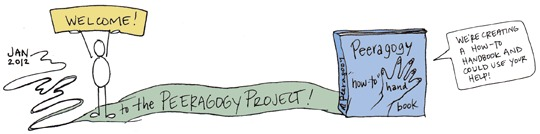
\includegraphics[width=.9\textwidth]{../pictures/welcome_color.jpg}
\end{center}

\subsection{Hello and welcome!}

The peeragogy project was kicked off around the time of
\href{http://rheingold.com/}{Howard Rheingold's} January 23, 2012
\href{http://vimeo.com/35685124}{Regents Lecture} at UC Berkeley on
\emph{Social Media and Peer Learning: From Mediated Pedagogy to
Peeragogy}. We have put together a handbook about peer learning: you're
reading it -- maybe on \href{peeragogy.org}{our website}, or in your
hammock with the beverage of your choice and our
\href{http://www.lulu.com/shop/howard-rheingold-and-peeragogyorg-editors/the-peeragogy-handbook/paperback/product-20607425.html}{print
on demand} paperback. Or maybe you grabbed our
\href{http://peeragogy.net/peeragogy-handbook-v1-1.pdf}{free PDF} or
some other remixed version in some other format or flavor from some
other place (which would be
\href{http://peeragogy.org/resources/license/}{cool}!).

But: there's still
\href{http://peeragogy.org/peeragogy-org-roadmap/}{more work to be
done}. We created this page because you might be interested in getting
involved in improving the book or furthering the project in other ways.
If so, we're happy to have you aboard!

What you do here is largely up to you. Asking questions is actually
extremely helpful: there's almost always someone in our
\href{https://plus.google.com/u/0/communities/107386162349686249470}{Google+
community} who would be happy to try to answer them, or refer you to
someone else who can.  Or just poke around the public pages on peeragogy.org and
leave a comment or two. Better still, find an area where you feel
knowledgeable -- or are willing to learn -- and start writing (or
filming, dancing, drawing, building, etc.).

\begin{center}
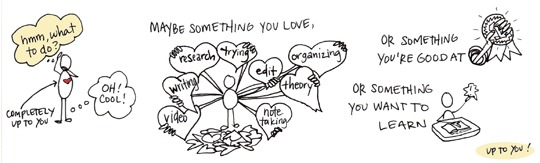
\includegraphics[width=.9\textwidth]{../pictures/what_to_do_color.jpg}
\end{center}

The goal we have in mind for our book is for it be a useful guide to
peer learning! To achieve that goal we have in mind multiple
opportunities for peers to contribute:

\begin{itemize}
\item
  Once we get to know you a little bit we'll be happy to give you a
  login on peeragogy.org and you can start editing and improving this.
\item
  You can go right ahead and post some links to relevant resources,
  either in comments here, or in the G+ or SMC.
\item
  Write the text for a new sub-section (this page was once ``new'' --
  but it's been revised many times by now!).
\item
  We're particularly interested in case studies about
  \href{http://peeragogy.org/peeragogy-in-action/}{Peeragogy in Action}!
\item
  Organize a team to tackle a larger section or topic.
\item
  Make a video (like these on our
  \href{http://www.youtube.com/channel/UCIQY4ja8e4Br-i9U5KnmyZQ}{YouTube
  Channel}),
\item
  Take notes of live meetings, or
  \href{http://cmapspublic3.ihmc.us/rid=1K81VLSK7-1RL0RQ4-WZK/Peeragogy\%20Cmap.cmap}{grow
  concept maps,}
\item
  Organize a newsletter for your group or the whole team,
\item
  Add general purpose bookmarks to
  \href{http://groups.diigo.com/group/peeragogy-handbook}{this Diigo
  group}, or post comments and editorial notes about peeragogy.org in
  \href{http://groups.diigo.com/group/peering-into-peeragogy\%20}{this
  one}; and
\item
  Discuss peer learning matters and this handbook informally with us and
  with others!
\end{itemize}
It's up to you. Instead of worrying too much about
\href{http://peeragogy.org/co-working/}{the rules}, join our
conversations, take advantage of the digital memory of the forum to
rewind the conversation all the way to the beginning (if you want to go
that far), listen in for a little bit if you want to, and jump in
whenever you're ready. We won't know what you're up to until you speak
up. You can have a look at the outstanding tasks and teams that are
listed on
\href{https://docs.google.com/document/d/1\_2I-z-Pt5NUKk-fpy4jsqxFeXbWS4ao4sIhkxCcRVeI/edit\#}{this
Google Doc}: our
\href{http://peeragogy.org/peeragogy-org-roadmap/}{roadmap} is a useful
shared resource too. You can add to these at any time.

We regularly use Google+, Google Hangouts, forums, and email to
communicate asynchronously and pretty much continuously. We also meet
irregularly as a group for synchronous audio-video sessions. Further
details about all these methods of communication can be found below.

In short: here's how it works:


\begin{center}

\includegraphics{../pictures/questions.jpg} \\
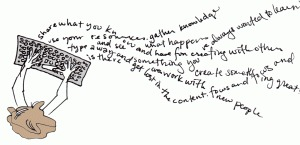
\includegraphics{../pictures/create_content.jpg} \\

\includegraphics{../pictures/communicate.jpg} \\
\end{center}

\subsection{Questions?}

If you have questions, that's good! Use Google+ or the forums, post a
comment on peeragogy.org, email the team energy center if you know who that
is, or email \href{mailto:howard@rheingold.com}{howard@rheingold.com}.

%
\chapter[\textbf{Peeragogy in Action}]{Peeragogy in Action}
%
We have been writing the missing manual for peer-produced peer
learning -- the ``Peeragogy Handbook''
(\href{http://peeragogy.org/}{peeragogy.org}).  While building this
book, we,~ourselves peer learners in this quest,~have been mindful of
these four questions:

\begin{enumerate}
\itemsep1pt\parskip0pt\parsep0pt
\item
  \emph{How does a motivated group of self-learners choose a subject or
  skill to learn?~}
\item
  \emph{How can this group identify and select the best learning
  resources about that topic?~}
\item
  \emph{How will these learners identify and select the appropriate
  technology and communications tools and platforms to accomplish their
  learning goal?}
\item
  \emph{What does the group need to know about learning theory and
  practice to put together a successful peer-learning program?}
\end{enumerate}

It is clear to us that the techniques of peer production that have built
and continue to improve \emph{Wikipedia} and GNU/Linux have yet to fully
demonstrate their power in education. We believe that the
\emph{Peeragogy Handbook} can help change that by building a distributed
community of peer learners/educators, and a strongly vetted collection
of best practices. Our project complements others' work on sites like
Wikiversity and P2PU, and builds upon understandings that have
developed informally in distributed communities of hobbyists and
professionals, as well as in (and beyond) the classrooms of
generations of passionate educators. Here, we present Peeragogy in
Action, a project guide in four parts. Each part relates to one or
more sections of our handbook, and suggests activities to try while
you explore peer learning. These activities are designed for flexible
use by widely distributed groups, collaborating via a light-weight
infrastructure. Participants may be educators, community organizers,
designers, hackers, dancers, students, seasoned peeragogues, or
first-timers. The guide should be useful for groups who want to build
a strong collaboration, as well as to facilitators or theorists who
want to hone their practice or approach.  Together, we will use our
various talents to build effective methods and models for peer
produced peer learning. Let's get started!


\noindent\raisebox{-2.7in}{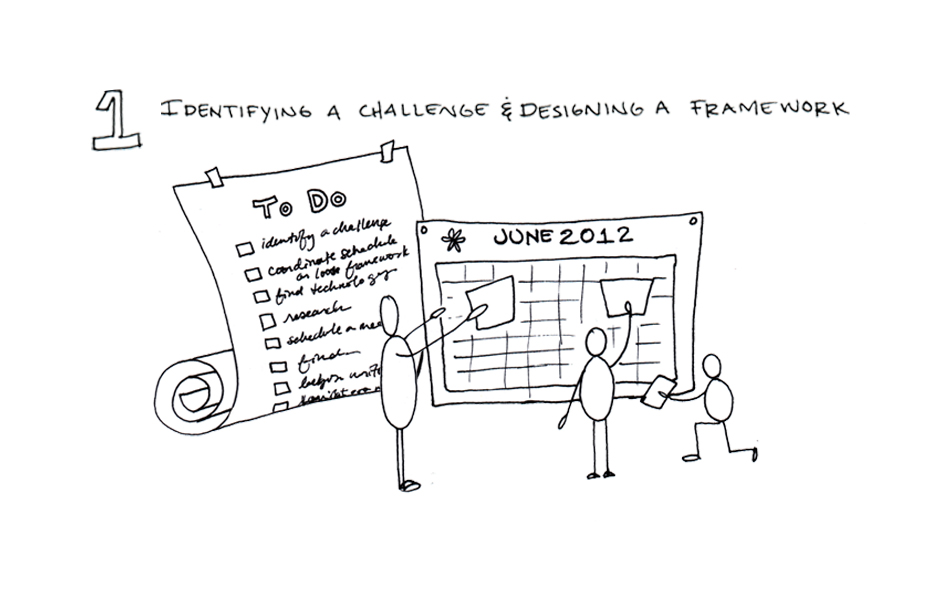
\includegraphics[width=.25\textwidth]{../pictures/OpenBook-2-1.jpg}}

\textbf{Setting the initial challenge and building a framework for
accountability among participants is an important starting point.}

\emph{Activity} -- Come up with a plan for your work and an agreement,
or informal contract, for your group. You can use the suggestions in
this guide as a starting point, but your first task is to revise the
plan to suit your needs. It might be helpful to ask: What are you
interested in learning? What is your primary intended outcome? What
problem do you hope to solve? ~How collaborative does your project need
to be? How will the participants' expertise in the topic vary? What sort
of support will you and other participants require? What problems won't
you solve?

\emph{Technology} -- Familiarize yourself with the collaboration tools
you intend to use (e.g. WordPress, Git and LaTeX, YouTube, GIMP, a
public wiki, a private forum, or something else) and create a first
post, edit, or video introducing yourself and your project(s) to others
in the worldwide peeragogy community.

\emph{Suggested Resources} -- The Peeragogy Handbook, parts I
(`\href{http://peeragogy.org/}{Introduction}') and II
(`\href{http://peeragogy.org/motivation/}{Motivation}'). You may
also want to work through a short lesson called
\href{https://en.wikiversity.org/wiki/User:Arided/ImplementingParagogy}{Implementing
Paragogy},~from the early days before the Peeragogy project was
convened. For a succinct theoretical treatment, please refer to our
literature review, which we have adapted into a
\href{http://en.wikipedia.org/wiki/Peer_learning}{Wikipedia page}.

\emph{Further Reading} -- Boud, D. and Lee, A. (2005). \emph{`Peer
learning' as pedagogic discourse for research education}. Studies in
Higher Education, 30(5):501--516.

\emph{Observations from the Peeragogy project} -- We had a fairly weak
project structure at the outset, which yielded mixed results. One
participant said: ``I definitely think I do better when presented with a
framework or scaffold to use for participation or content development.''
Yet the same person wrote with enthusiasm about models of
entrepreneurship, saying she was ``freed of the requirement or need for
an entrepreneurial visionary.'' 

\noindent\raisebox{-2.7in}{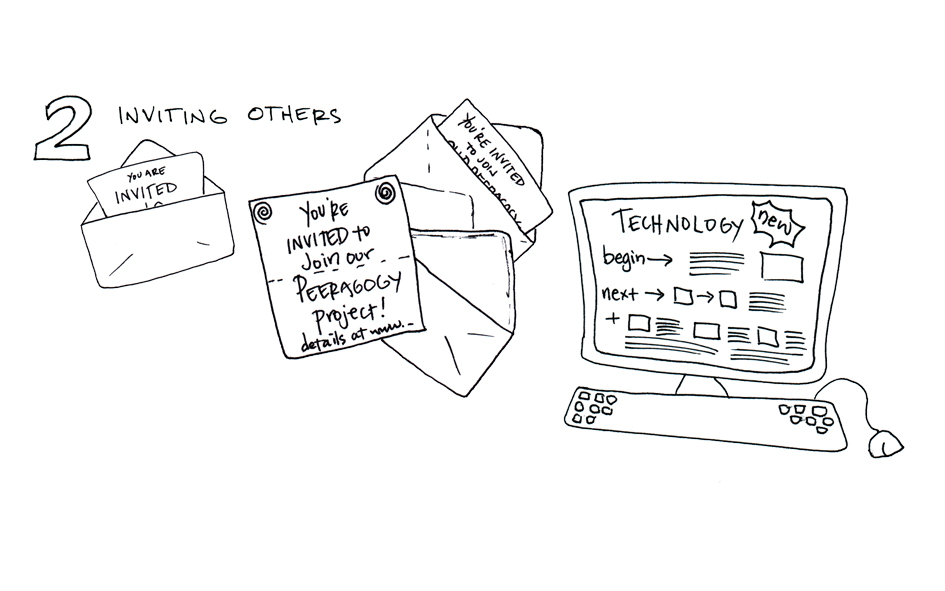
\includegraphics[width=.25\textwidth]{../pictures/OpenBook-2-2.jpg}}

\textbf{Other people can support you in achieving your goal and make the
work more fun too.}

\emph{Activity} -- Write an invitation to someone who can help as a
co-facilitator on your project. Clarify what you hope to learn from them
and what your project has to offer. Helpful questions to consider as you
think about who to invite: What resources are available or missing? What
do you already have that you can build on? How will you find the
necessary resources? Who else is interested in these kinds of
challenges? Go through the these questions again when you have a small
group, and come up with a list of more people you'd like to invite or
consult with as the project progresses.

\emph{Technology} -- Identify tools that could potentially be useful
during the project, even if it's new to you. Start learning how to use
them. Connect with people in other locales who share similar interests
or know the tools.

\emph{Suggested resources} -- The Peeragogy Handbook, parts IV
(`\href{http://peeragogy.org/convening-a-group/}{Convening a Group}')
and V
(`\href{http://peeragogy.org/organizing-a-learning-context/}{Organizing
a Learning Context}').

\emph{Recommended Reading} -- Schmidt, J. Philipp. (2009). Commons-Based
Peer Production and education. Free Culture Research Workshop Harvard
University, 23 October 2009.

\emph{Observations from the Peeragogy project} -- We used a strategy of
``open enrollment.'' New people were welcome to join the project at any
time. We also encouraged people to either stay involved or withdraw;
several times over the first year, we required participants to
explicitly reaffirm interest in order to stay registered in the forum
and mailing list.

\noindent\raisebox{-2.7in}{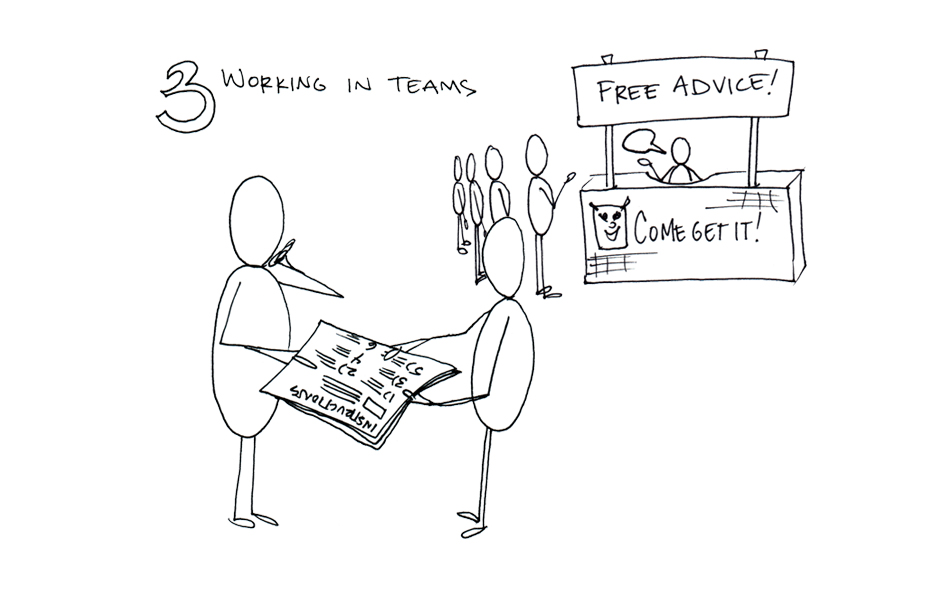
\includegraphics[width=.25\textwidth]{../pictures/OpenBook-2-3.jpg}}

\textbf{Solidifying your work plan and learning strategy together with
concrete measures for `success' can move the project forward
significantly.}

\emph{Activity} -- Distill your ideas by writing an essay, making visual
sketches, or creating a short video to communicate the unique plans for
organization and evaluation that your group will use. By this time, you
should have identified which aspects of the project need to be refined
or expanded. Dive in!

\emph{Technology} -- Take time to mentor others or be mentored by
someone, meeting up in person or online. Pair up with someone else and
share knowledge together about one or more tools. You can discuss some
of the difficulties that you've encountered, or teach a beginner some
tricks.

\emph{Suggested resources} -- The Peeragogy Handbook, parts VI
(`\href{http://peeragogy.org/co-facilitation/}{Cooperation}'), VII
(`\href{http://peeragogy.org/assessment/}{Assessment}'), and at least some of part II
(`\href{http://peeragogy.org/patterns-usecases/}{Peeragogy in Practice}').

\emph{Recommended reading} -- Argyris, Chris. ``Teaching smart people
how to learn.'' Harvard Business Review 69.3 (1991); and, Gersick,
Connie J.G. ``Time and transition in work teams: Toward a new model of
group development.'' Academy of Management Journal 31.1 (1988): 9-41.

\emph{Observations from the Peeragogy project} -- Perhaps one of the
most important roles in the Peeragogy project was the role of the
`Wrapper', who prepared and circulated weekly summaries of forum
activity. This helped people stay informed about what was happening in
the project even if they didn't have time to read the forums. We've also
found that small groups of people who arrange their own meetings are
often the most productive.

\noindent\raisebox{-2.7in}{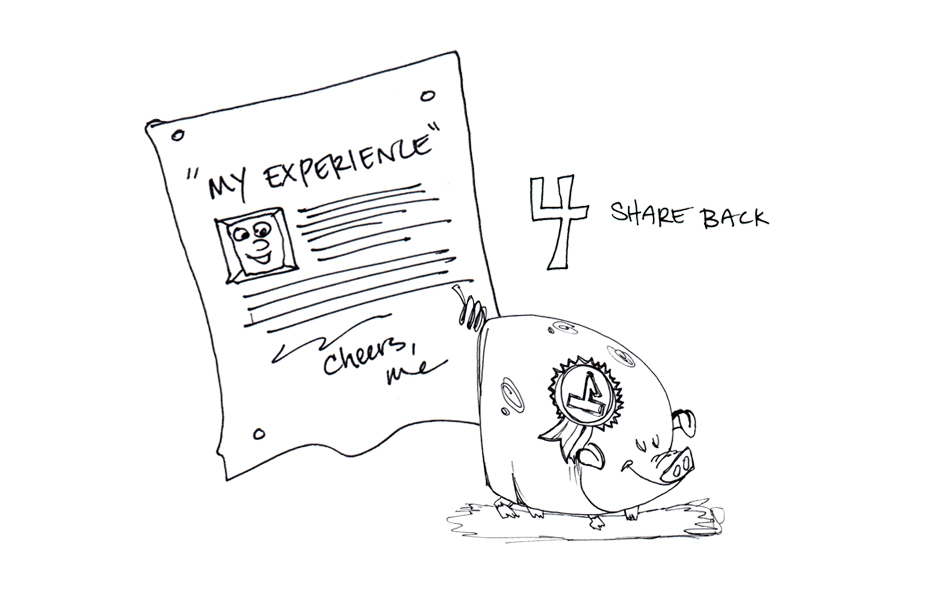
\includegraphics[width=.3\textwidth]{../pictures/OpenBook-2-4.jpg}}

\textbf{Wrap up the project with a critical assessment of progress and
directions for future work. Share any changes to this syllabus that you
think would be useful for future peeragogues!}

\emph{Activity} -- Identify the main obstacles you encountered. What are
some goals you were not able to accomplish yet? Did you foresee these
challenges at the outset? How did this project resemble or differ from
others you've worked on? How would you do things differently in future
projects? What would you like to tackle next?

\emph{Writing} -- Communicate your reflection case. Prepare a short
written or multimedia essay, dealing with your experiences in this
course. Share the results by posting it where others in the broader
Peeragogy project can find it.

\emph{`Extra credit'} -- Contribute back to one of the other
organisations or projects that helped you on this peeragogical journey.
Think about what you have to offer. Is it a bug fix, a constructive
critique, pictures, translation help, PR, wiki-gnoming or making a cake?
Make it something special, and people will remember you and thank you
for it.

\emph{Suggested resources} -- The Peeragogy Handbook, parts VIII
(`\href{http://peeragogy.org/resources/technologies/}{Technologies,
Services, and Platforms}') and IX
(`\href{http://peeragogy.org/resources/}{Resources}').

\emph{Recommended reading} -- Stallman, Richard.
``\href{http://www.gnu.org/philosophy/shouldbefree.html}{Why software
should be free}'' (1992).

\emph{Observations from the Peeragogy project} -- When we were deciding
how to license our work,~ we decided to use CC0, emphasizing~
`re-usability' and hoping that other people would come and remix the
handbook.~ At the moment, we're still waiting to see the first remix
edition, but we're confident that it will come along in due course.~
Maybe you'll be the one who makes it!

\subsection{{\tiny Micro-}Case Study: The Peeragogy Project, Year 1}

Since its conception in early 2012, the Peeragogy Project has collected
over 3700 comments in our discussion forum, and over 200 pages of
expository text in the handbook. It has given contributors a new way of
thinking about things together. However, the project has not had the
levels of engagement that should be possible, given the technology
available, the global interest in improving education, and the number of
thoughful participants who expressed interest. We hope that the handbook
and this accompanying syllabus will provide a seed for a new phase of
learning, with many new contributors and new ideas drawn from real-life
applications.

\subsection{{\tiny Micro-}Case Study: The Peeragogy Project, Year 2}

10 new handbook contributors joined in the project's second year. We've
begun a series of weekly Hangouts on Air that have brought in many
additional discussants, all key people who can help to fulfil
peeragogy's promise.~ The handbook has been considerably improved
through edits and discussion.~ The next step for us is putting this work
into action in the \emph{Peeragogy Accelerator}.

\subsection{{\tiny Micro-}Case Study: The Peeragogy Project, Year 3}

We published our plans as ``Building the Peeragogy Accelerator'',
presenting it at OER14 and inviting feedback.  However, we failed to
recruit any newcomers for the trial run.  Piloting the Accelerator
with some of our own projects worked reasonably well,\footnote{For an
overview, see \url{http://is.gd/up_peeragogy_accelerator}.} but we
decided to focus on the handbook in the second half of the year.  As
the project's line-up shifted, participants reaffirmed the importance
of having ``no camp counsellors.''  In the last quarter of 2015,
we created the workbook that is now presented in Part I, as a
quickstart guide to peeragogy.

% 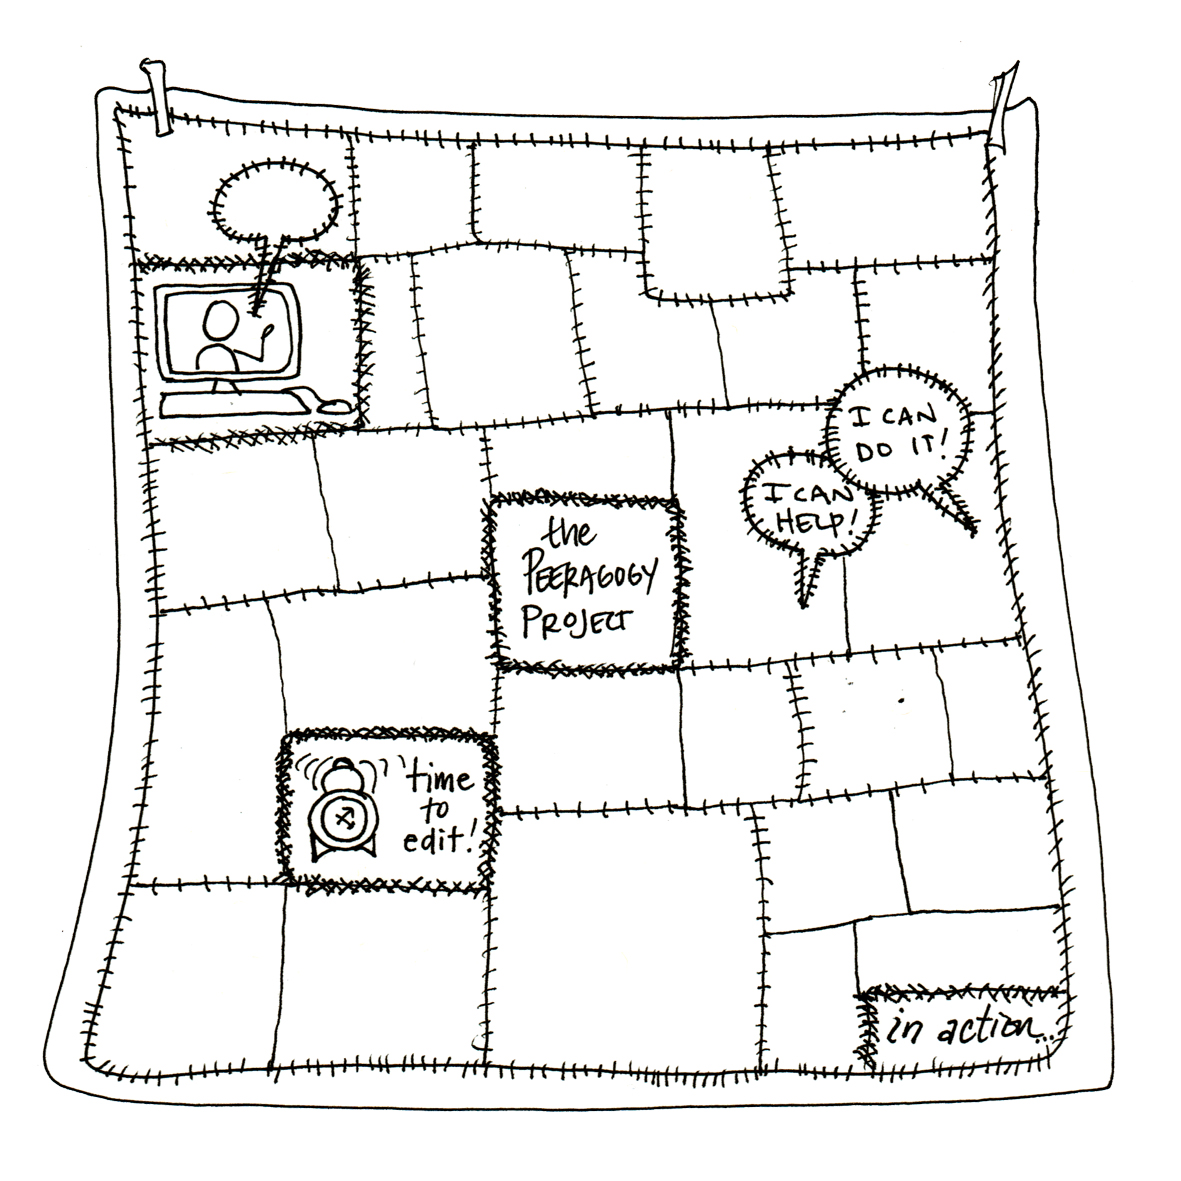
\includegraphics[width=.3\textwidth]{../pictures/OpenBook-3.jpg}

%
\chapter[\textbf{Recommended Reading}]{Recommended Reading}
%
\subsection{``Good faith
collaboration''}\label{rec:good-faith-collaboration}

\begin{enumerate}
\def\labelenumi{\arabic{enumi}.}
\itemsep1pt\parskip0pt\parsep0pt
\item
  Reagle, J.~M. (2010). Good faith collaboration: The culture of
  Wikipedia, MIT Press.
\end{enumerate}

\subsection{Writings about fun and
boredom}\label{rec:writings-about-fun-and-boredom}

\begin{enumerate}
\def\labelenumi{\arabic{enumi}.}
\item
  Kano, J. (1995/2013). \href{http://judoinfo.com/kano.htm}{The
  Contribution of Judo to Education}.
\item
  Pale King, unfinished novel, by David Foster Wallace
\item
  On the Poverty of Student Life, by Mustapha Khayati
\end{enumerate}

\subsection{The structure of learning}\label{rec:the-structure-of-learning}

Check out work by Bruce Tuckman, Gilly Salmon, Ken Wilber, Martin
Oliver, Gráinne Conole, Ruth Deakin-Crick, Howard Gardner, and Mihaly
Csíkszentmihályi.

\subsection{Motivation}\label{rec:motivation}

\begin{enumerate}
\def\labelenumi{\arabic{enumi}.}
\itemsep1pt\parskip0pt\parsep0pt
\item
  Simon Sinek, Start With Why: How Great Leaders Inspire Everyone To
  Take Action, Penguin Books, 2011
\end{enumerate}

\subsection{Case Study: 5PH1NX}\label{rec:case-study-5ph1nx}

\begin{enumerate}
\def\labelenumi{\arabic{enumi}.}
\itemsep1pt\parskip0pt\parsep0pt
\item
  Senge, Peter. ``The fifth discipline: The art and science of the
  learning organization.'' \emph{New York: Currency Doubleday} (1990).
\end{enumerate}

\subsection{Alexandrian Design
Patterns}\label{rec:alexandrian-design-patterns}

\begin{enumerate}
\def\labelenumi{\arabic{enumi}.}
\item
  Article, ``Manifesto 1991'' by Christopher Alexander, Progressive
  Architecture, July 1991, pp.~108--112, provides a brief summary of
  Alexander's ideas in the form of a critique of mainstream
  architecture. Many of the same sorts of critical points would carry
  over to mainstream education. Some highlights are excerpted
  \href{https://plus.google.com/u/0/108598104736826154120/posts/agWYcqPhqSN}{here}.
\item
  \href{http://www.patternlanguage.com/archive/ieee/ieeetext.htm}{The
  Origins of Pattern Theory, the Future of the Theory, And The
  Generation of a Living World}, Christopher Alexander's talk at the
  1996 ACM Conference on Object-Oriented Programs, Systems, Languages
  and Applications (OOPSLA)
\end{enumerate}

\subsection{On Newcomers}\label{rec:on-newcomers}

\begin{enumerate}
\def\labelenumi{\arabic{enumi}.}
\item
  OpenHatch.org, ``an open source community aiming to help newcomers
  find their way into free software projects.''
\item
  \href{http://lapessc.ime.usp.br/public/papers/13872/CHASE13_present.pdf}{Why
  do newcomers abandon open source software projects?} (sildes by Igor
  Steinmacher and coauthors)
\end{enumerate}

\subsection{Antipatterns}\label{rec:antipatterns}

\begin{enumerate}
\def\labelenumi{\arabic{enumi}.}
\item
  The
  \href{http://en.wikipedia.org/wiki/Linguistic_relativity}{Sapir-Whorf
  Hypothesis}
\item
  Bourdieu's notion of
  ``\href{http://en.wikipedia.org/wiki/Symbolic_violence}{symbolic
  violence}''.
\end{enumerate}

\subsection{SWATs}\label{rec:swats}

\begin{enumerate}
\def\labelenumi{\arabic{enumi}.}
\itemsep1pt\parskip0pt\parsep0pt
\item
  Cavallo, David. ``Emergent design and learning environments: Building
  on indigenous knowledge.'' IBM Systems Journal 39.3.4 (2000): 768-781.
\end{enumerate}

\subsection{Convening a Group}\label{rec:convening-a-group}

\begin{enumerate}
\def\labelenumi{\arabic{enumi}.}
\item
  Engeström, Y. (1999). Innovative learning in work teams: Analyzing
  cycles of knowledge creation in practice. In Y. Engeström, R.
  Miettinen \& R.-L-. Punamäki (Eds.), \emph{Perspectives on activity
  theory}, (pp.~377-404). Cambridge, UK: Cambridge University Press
\item
  Gersick, C. (1988). Time and transition in work teams: Toward a new
  model of group development. \emph{Academy of Management Journal} 31
  (Oct.): 9-41.
\item
  Mimi Ito's observations about
  \href{http://mitpress.mit.edu/books/full_pdfs/hanging_out.pdf}{manga
  fan groups co-learning Japanese}
\item
  Rheingold U,
  \href{http://socialmediaclassroom.com/host/mindamp5/lockedwiki/main-page}{MindAmp
  groups}
\item
  Shneiderman, B. (2007).
  \href{http://doi.acm.org/10.1145/1323688.1323689}{Creativity support
  tools: accelerating discovery and innovation}. \emph{Commun. ACM} 50,
  12 (December 2007), 20-32.
\item
  David de Ugarte, Phyles.
  (\href{http://david.lasindias.com/phyles/}{Summary})
  (\href{http://deugarte.com/gomi/phyles.pdf}{Book})
\item
  Scheidel, T. M., \& Crowell, L. (1964). Idea development in small
  discussion groups. \emph{Quarterly Journal of Speech}, 50, 140-145.
\item
  Scheidel, T. M., \& Crowell, L. (1979), \emph{Discussing and Deciding
  - A Desk Book for Group Leaders and Members}, Macmillan Publishing
\item
  Ozturk and Simsek, ``Of Conflict in Virtual Learning Communiities in
  the Context of a Democratic Pedagogy: A paradox or sophism?,'' in
  \emph{Proceedings of the Networked Learning Conference, 2012,
  Maastricht.}
  \href{http://www.google.com/search?client=chrome-mobile\&sourceid=chrome-mobile\&ie=UTF-8\&q=Of+Conflict+in+Virtual+Learning+Communiities+in+the+Context+of+a+Democratic+Pedagogy}{Video}
  or
  \href{http://networkedlearningconference.org.uk/abstracts/pdf/ozturk.pdf}{text}.
\item
  Paragogy Handbook,
  \href{http://peeragogy.org/organizing-a-learning-context/connectivism-in-practice-how-to-organize-a-mooc/}{How
  to Organize a MOOC}
\item
  Cathy Davidson et al.,
  \href{http://news.rapgenius.com/Cathy-davidson-how-a-class-becomes-a-community-theory-method-examples-chapter-one-lyrics}{How
  a Class Becomes a Community}
\end{enumerate}

\subsection{K-12 Peeragogy}\label{rec:k-12-peeragogy}

\subsubsection{For pointers to tools for your classroom, check
out:}\label{rec:for-pointers-to-tools-for-your-classroom-check-out}

\begin{itemize}
\itemsep1pt\parskip0pt\parsep0pt
\item
  \href{http://www.freetech4teachers.com/}{Richard Byrne}
\item
  \href{http://langwitches.org/blog/}{Sylvia Tolisano}
\item
  \href{http://catlintucker.com/2011/11/12-tech-tools-that-will-transform-your-classroom/}{Caitlin
  Tucker}
\item
  \href{http://coolcatteacher.blogspot.ca/}{Vicki Davis}
\end{itemize}

\subsubsection{How to develop your PLN:}\label{rec:how-to-develop-your-pln}

\begin{itemize}
\itemsep1pt\parskip0pt\parsep0pt
\item
  \href{\%20http://thecleversheep.blogspot.ca/2012/06/seven-degrees-of-connectedness_06.html}{Degrees
  of Connected Teaching} by Rodd Lucier
\item
  \href{\%20http://thecleversheep.blogspot.ca/2012/06/seven-degrees-of-connectedness_06.html}{TeachThought}
\end{itemize}

\subsubsection{Theory \& philosophy of connnected learning for classroom
transformation:}\label{rec:theory-philosophy-of-connnected-learning-for-classroom-transformation}

\begin{itemize}
\itemsep1pt\parskip0pt\parsep0pt
\item
  \href{http://pairadimes.davidtruss.com/}{David Truss}
\item
  \href{http://www.downes.ca/presentation/264}{Steven Downes}
\item
  \href{http://willrichardson.com/}{Will Richardson}
\end{itemize}

\subsection{Adding Structure with
Activities}\label{rec:adding-structure-with-activities}

\begin{enumerate}
\def\labelenumi{\arabic{enumi}.}
\item
  \href{http://dschool.stanford.edu/wp-content/uploads/2011/03/BootcampBootleg2010v2SLIM.pdf}{The
  d.school Bootcamp Bootleg} (CC-By-NC-SA) includes lots of fun
  activities to try. Can you crack the code and define new ones that are
  equally cool?
\item
  Puzio, R. S. (2005). ``On free math and copyright bottlenecks.''
  \emph{Free Culture and the Digital Library Symposium Proceedings}.
\end{enumerate}

\subsection{Co-Facilitation}\label{rec:co-facilitation}

\begin{enumerate}
\def\labelenumi{\arabic{enumi}.}
\item
  \href{http://www.scribd.com/doc/54544925/51/TRAINING-TOPIC-Co-facilitation-skills}{Peer
  Education: Training of Trainers Manual}; UN Interagency Group on Young
  Peoples Health
\item
  \href{http://www.breakoutofthebox.com/Co-FacilitatingPfeifferJones.pdf}{Co
  Facilitating}: Advantages \& Potential Disadvantages. J. Willam
  Pfeifer and John E Johnes
\item
  \href{http://reviewing.co.uk/archives/art/13_1_what_do_facilitators_do.htm\#8_WAYS_OF_FACILITATING_ACTIVE_LEARNING}{Summary}
  of John Heron's model of the role of facilitators
\item
  \href{http://www.infed.org/thinkers/et-rogers.htm}{Carl Rogers, Core
  Conditions and Education}, Encyclopedia of Informal Education
\item
  \href{http://www.studygs.net/peermed.htm}{Peer Mediation}, Study
  Guides and Strategies
\item
  \href{http://sk.cupe.ca/updir/cofacilitation-handouts.doc}{Co-Facilitation:
  The Advantages and Challenges}, Canadian Union of Public Employees
\item
  \href{http://community.bistudio.com/wiki/Bohemia_Interactive_Community:Guidelines}{Bohemia
  Interactive Community Wiki Guidelines}
\item
  Barrett-Lennard, G. T. (1998) Carl Roger's Helping System.  Journey
  and Substance.  London: Sage
\item
  \href{http://en.wikipedia.org/w/index.php?title=Wikipedia:Five_pillars\&oldid=501472166}{5
  Pillars of Wikipedia}, from Wikipedia
\item \emph{\href{http://www.africom.mil/WO-NCO/DownloadCenter/\%5C40Publications/Training\%20the\%20Force\%20Manual.pdf}{Training
  the Force}}, US Army Field Manual \#FM 7-0 (FM 25-100)
\item
  \href{http://dmlcentral.net/blog/howard-rheingold/learning-reimagined-participatory-peer-global-online}{Learning
  Reimagined: Participatory, Peer, Global, Online}, by Howard Rheingold
\item
  \href{http://www.researchgate.net/}{Research Gate} is a network
  dedicated to science and research, in which members connect,
  collaborate and discover scientific publications, jobs and
  conferences.
\item
  \href{http://ctb.ku.edu/en/tablecontents/section_1180.aspx}{Creating
  and Facilitating Peer Support Groups}, by The Community Tool Box
\item
  \href{http://www1.villanova.edu/content/villanova/artsci/vcle/resources/toolkit/_jcr_content/pagecontent/download_8/file.res/FacilitationTips.doc}{Facilitation
  Tips}, by Villanova University
\item
  \href{http://pippabuchanan.com/2011/09/04/herding-passionate-cats-the-role-of-facilitator-in-a-peer-learning-process/}{Herding
  Passionate Cats: The Role of Facilitator in a Peer Learning Process},
  by Pippa Buchanan
\item
  \href{http://webpages.sou.edu/~vidmar/SOARS2008/vidmar.ppt}{Reflective
  Peer Facilitation: Crafting Collaborative Self-Assessment}, by Dale
  Vidmar, Southern Oregon University Library
\item
  \href{http://www.umass.edu/ewc/ea/Facilitation\%20Skills/important\%20tips.doc}{Effective
  Co-Facilitation}, by Everywoman's Center, University of Massachussetts
\item
  ``\href{www.ncsu.edu/park_scholarships/pdf/chris_argyris_learning.pdf?}{Teaching
  smart people how to learn}'' by Chris Argyris, Harvard Business Review
  69.3, 1991; also published in expanded form as a
  \href{http://www.amazon.com/Teaching-People-Harvard-Business-Classics/dp/1422126005}{book}
  with the same name.
\end{enumerate}

\subsection{Assessment}\label{rec:assessment}

\begin{enumerate}
\def\labelenumi{\arabic{enumi}.}
\item
  Morgan, C. and M. O'Reilly. (1999).
  \href{http://www.amazon.com/Assessing-Distance-Learners-Flexible-Learning/dp/0749428783/ref=tmm_pap_title_0?ie=UTF8\&qid=1388199564\&sr=1-1}{Assessing
  Open and distance learners.} London: Kogan Page Limited.
\item
  Schmidt, J. P., Geith, C., Håklev, S. and J. Thierstein. (2009).
  \href{http://www.irrodl.org/index.php/irrodl/article/view/641/1389}{Peer-To-Peer
  Recognition of Learning in Open Education}. \emph{International Review
  of Research in Open and Distance Learning}. Volume 10, Number 5.
\item
  L.S. Vygotsky:
  \href{http://books.google.com/books?id=RxjjUefze_oC\&printsec=frontcover\&source=gbs_atb\#v=onepage\&q\&f=false}{Mind
  in Society: Development of Higher Psychological Processes}
\item
  \href{http://org.sagepub.com/search?author1=Reijo+Miettinen\&sortspec=date\&submit=Submit}{Reijo
  Miettinen} and
  \href{http://org.sagepub.com/search?author1=Jaakko+Virkkunen\&sortspec=date\&submit=Submit}{Jaakko
  Virkkunen},
  \href{http://org.sagepub.com/content/12/3/437.abstract}{Epistemic
  Objects, Artifacts and Organizational Change}, \emph{Organization,}
  May 2005, 12: 437-456.
\end{enumerate}

\subsection{Technologies, Services, and
Platforms}\label{rec:technologies-services-and-platforms}

\begin{enumerate}
\def\labelenumi{\arabic{enumi}.}
\item
  Irene Greif and Sunil Sarin (1987): Data Sharing in Group Work, ACM
  Transactions on Office Information Systems, vol.~5, no. 2, April 1987,
  pp.~187-211.
\item
  Irene Greif (ed.) (1988): Computer-Supported Cooperative Work: A Book
  of Readings, San Mateo, CA: Morgan Kaufman.
\item
  Irene Greif (1988): Remarks in panel discussion on ``CSCW: What does
  it mean?'', CSCW `88. Proceedings of the Conference on
  Computer-Supported Cooperative Work, September 26-28, 1988, Portland,
  Oregon, ACM, New York, NY.
\item
  Kammersgaard, J., Four Different Perspectives on Human-Computer
  Interaction. International Journal of Man-Machine Studies 28(4):
  343-362 (1988)
\item
  DeSanctis, G. and Poole, M. S. 1994, `Capturing the complexity in
  advanced technology use: Adaptive structuration theory', Organisation
  Science, vol.~5, no. 2, p.~121-47.
\item
  Norman, D. A. 1986, `Cognitive engineering', in Norman, D. A. and
  Draper, S. W., (eds) User Centered System Design: New Perspectives on
  Human-Computer Interaction, pp.~31-61. Hillsdale, NJ: Lawrence Erlbaum
  and Associates.
\item
  Vessey, I. and Galletta, D. 1991, `Cognitive fit: An empirical study
  of information acquisition', Information Systems Research, vol.~2, no.
  1, pp.~63-84.
\end{enumerate}

\subsubsection{Real-Time Meetings}\label{rec:real-time-meetings}

\begin{enumerate}
\def\labelenumi{\arabic{enumi}.}
\itemsep1pt\parskip0pt\parsep0pt
\item
  Howard Rheingold's webconferencing
  \href{http://delicious.com/hrheingold/webconferencing}{bookmarks} on
  Delicious.
\end{enumerate}

\subsubsection{Additional Tips from an open source
perspective}\label{rec:additional-tips-from-an-open-source-perspective}

Care of User:Neophyte on the Teaching Open Source wiki.

\begin{enumerate}
\def\labelenumi{\arabic{enumi}.}
\item
  The Art of Community
\item
  Open Advice
\item
  The Open Source Way
\end{enumerate}

\subsection{Forums}\label{rec:forums}

\begin{enumerate}
\def\labelenumi{\arabic{enumi}.}
\item
  Rheingold, H. \href{http://blip.tv/file/1123048}{Why use forums?}
  \emph{Social Media Classroom}.
\item
  Rheingold, H. (1998).
  \href{http://www.rheingold.com/texts/artonlinehost.html}{The Art of
  Hosting Good Conversations Online}.
\item
  Gallagher, E. J. (2006).
  \href{http://www.lehigh.edu/~indiscus/doc_guidelines.html}{Guidelines
  for Discussion Board Writing}. Lehigh University.
\item
  Gallagher, E.J. (2009).
  \href{http://www.academiccommons.org/2009/01/shaping-a-culture-of-conversation-the-discussion-board-and-beyond/}{Shaping
  a culture of conversation. The discussion board and beyond}. The
  Academic Commons.
\item
  Academic Technology Center. (2010).
  \href{http://www.wpi.edu/Academics/ATC/Collaboratory/Idea/boards.html}{Improving
  the Use of Discussion Boards}. Worcester Polytechnic Institute.
\end{enumerate}

\subsection{Paragogy}\label{rec:paragogy}

\begin{enumerate}
\def\labelenumi{\arabic{enumi}.}
\item
  Corneli, J. (2010).
  \href{http://metameso.org/~joe/docs/paragogy-lesson.pdf}{Implementing
  Paragogy}, on \emph{Wikiversity}.
\item
  Corneli, J. and C. Danoff. (2010/2013). \emph{Paragogy.net}.
\end{enumerate}

\subsection{Learning vs Training}\label{rec:learning-vs-training}

\begin{enumerate}
\def\labelenumi{\arabic{enumi}.}
\itemsep1pt\parskip0pt\parsep0pt
\item
  Hart, J. (April 20th, 2012).
  \href{http://www.c4lpt.co.uk/blog/2012/04/20/is-it-time-for-a-byol-bring-your-own-learning-strategy-in-your-organization-byol/}{Is
  it time for a BYOL (Bring Your Own Learning) strategy for your
  organization?} \emph{Learning in the Social Space. Jane Hart's Blog.}
\end{enumerate}

\subsection{PLNs}\label{rec:plns}

\begin{enumerate}
\def\labelenumi{\arabic{enumi}.}
\item
  Rheingold, H. (2010).
  \href{http://dmlcentral.net/blog/howard-rheingold/shelly-terrell-global-netweaver-curator-pln-builder}{Shelly
  Terrell: Global Netweaver, Curator, PLN Builder.} \emph{DML Central}.
\item
  Richardson, W. and R. Mancabelli. (2011).
  \href{http://www.amazon.com/Personal-Learning-Networks-Connections-Transform/dp/193554327X}{Personal
  Learning Networks: Using the Power of Connection to Transform
  Education}. Bloomington, IN: Solution Tree Press.
\item
  Howard Rheingold's PLN links on Delicious
\end{enumerate}

\subsection{Connectivism in Practice --- How to Organize a MOOC (Massive
Open Online
Class)}\label{rec:connectivism-in-practice-how-to-organize-a-mooc-massive-open-online-class}

\begin{enumerate}
\def\labelenumi{\arabic{enumi}.}
\item
  Downes \& Siemens \href{http://change.mooc.ca}{MOOC site}
\item
  \href{http://halfanhour.blogspot.com/2007/02/what-connectivism-is.html}{What
  Connectivism Is} by Stephen Downes
\item
  \href{http://www.downes.ca/post/33034}{An Introduction to Connective
  Knowledge} by Stephen Downes
\item
  \href{http://www.downes.ca/presentation/290}{Facilitating a Massive
  Open Online Course}, by Stephen Downes
\item
  \href{http://grsshopper.downes.ca/index.html}{gRSShopper}
\item
  \href{\%20http://www.elearnspace.org/Articles/connectivism.htm}{Connectivism:
  A Learning Theory for the Digital Age} by George Siemens
\item
  \href{http://en.wikiversity.org/wiki/Connectivism_glossary}{A
  Connectivism Glossary}
\item
  \href{http://www.connectivism.ca/?p=329}{Rhizomes and Networks} by
  George Siemens
\item
  \href{http://innovateonline.info/pdf/vol4_issue5/Rhizomatic_Education-__Community_as_Curriculum.pdf}{Rhizomatic
  Education: Community as Curriculum} by Dave Cormier
\item
  \href{http://www.amazon.ca/Knowing-Knowledge-George-Siemens/dp/1430302305}{Knowing
  Knowledge}, a book by George Siemens
\item
  \href{http://www.amazon.com/Net-Smart-ebook/dp/B007D5UP9G}{Net Smart,}
  Howard Rheingold (about internal and external literacies for coping
  with the `always on' digital era)
\item
  \href{http://www.learningsolutionsmag.com/articles/886/}{Massive Open
  Online Courses}: Setting Up (StartToMOOC, Part 1)
\item
  \href{https://sites.google.com/site/themoocguide/}{The MOOC guide}
\end{enumerate}

\subsubsection{And, a word list for your inner
edu-geek}\label{rec:and-a-word-list-for-your-inner-edu-geek}

You can read about all of these things on Wikipedia.

\begin{enumerate}
\def\labelenumi{\arabic{enumi}.}
\item
  \href{http://en.wikipedia.org/wiki/Constructivism_(philosophy_of_education)}{Constructivism}
\item
  \href{http://en.wikipedia.org/wiki/Social_constructivism}{Social
  constructivism}
\item
  \href{http://www.english.iup.edu/mmwimson/Syllabi/803/721/Radical\%20Constructivism\%20\%20\%20721.htm}{Radical
  constructivism}
\item
  \href{http://en.wikipedia.org/wiki/Enactivism_(psychology)}{Enactivism}
\item
  \href{http://en.wikipedia.org/wiki/Constructionism_(learning_theory)}{Constructionism}
\item
  \href{http://en.wikipedia.org/wiki/Connectivism}{Connectivism}
\end{enumerate}

%
\chapter[\textbf{Style Guide}]{Style Guide}
%
{\centering\emph{This is a How-To Handbook.}\par}

\subsection{Keep it short}

The easiest sections to read are those that are shorter and include some
kind of visual (video or image) and have some personal connection (i.e.
they tell a story). For anything longer, break it up into sub-pages, add
visuals, make sure each sub-page is accessible to someone (who is it?).
Think clearly of this reader, talk to them.

\subsection{Make it clear}

We'll illustrate this point by example. The original full title of the
book was ``The Peeragogy Handbook: A resource for self-organizing
self-learners''. But
``\href{http://en.wikipedia.org/wiki/Self-organization}{self-organizing}''
is a technical term, and ``self-learner'' is a confusing neologism. We
shouldn't use technical terms unless we explain them. So we really
shouldn't use it in the first sentence or paragraph, or title, of the
book because we'll scare people off or confuse them. If we want to
explain what ``self-organization'' means and why it is relevant for
peeragogy, then we can take a chapter to do that much later on in the
book. At the same time, we shouldn't try to ``say the same thing in a
simpler way.'' We should try to get rid of the technical concept
completely and see what's left. The easiest thing to do in such cases is
to delete the sentence completely and start over: when in doubt, speak
plainly.

\subsection{Don't overdo it with bullet points}

Text can be very hard to read when there are more than a few bullet
points included. Numbered lists should also be used sparingly. It also
seems that when many disjointed bullet points appear, sometimes the
author is really just indexing the main points that are presented better
in someone else's narrative. Therefor, consider replacing an entire
bulleted list with a reference to someone else's book/webpage/chapter.
In today's hyperlinked world, it's easy enough for the reader to go
elsewhere to get good content (and indeed, we should make it easy for
them to find the best treatments around!). It is not very pleasant to
have to \emph{read} a taxonomy.

\subsection{Include activities}

When reading, editing or otherwise working your way through the book,
please make note of any activities or exercises that come to mind, and
share them.~ We're always striving to be more practical and applicable.

\subsection{Don't be overly chatty}

In our efforts to escape from academia-speak and simplify the text in
the handbook, it's important to make sure we are not heading towards the
other extreme -- being too conversational. When we're having a
conversation with someone, we tend to pepper our ideas with transitional
or pivotal phrases (``In any event,'' ``With that said,'' ``As I
mentioned elsewhere,'' etc.) that help to keep the talk flowing. We also
go off on brief tangents before making our way back to the main topic,
and sometimes express ourselves in run-on sentences. While this is
perfectly natural in speech, it can be confusing and complex in written
text. Let's strive for the perfect balance of simple yet professional
writing.

\subsection{Bonus points}

Capitalize the first word of each item in a bulleted list, especially
if items include a verb form.~ Punctuate
uniformly.
Capitalize the first word of headings and subheadings; lower case all
others.

%% \subsection{Format your HTML nicely}

%% We need to be able to process the content from this Wordpress site and
%% turn it into various formats like LaTeX and EPUB. Our automated tools
%% work much better if pages are formatted with simple and uniform HTML
%% markup. Some key points:

%% \begin{itemize}
%% \itemsep1pt\parskip0pt\parsep0pt
%% \item
%%   Mark up your links: use~\href{http://peeragogy.org}{The Peeragogy
%%   Handbook}~instead
%%   of~\href{http://peeragogy.org}{http://peeragogy.org}.~ It's best if
%%   the link text is somewhat descriptive.
%% \item
%%   Use a numbered list to format your references
%%   (see~\href{http://peeragogy.org/convening-a-group/}{Convening a
%%   Group}~for one example of an article that gets this right!)
%% \item
%%   Use Heading 2 and Heading 3 tags to mark up sections,
%%   not~\textbf{bold}~text.~ If you use bold or italics in your
%%   paragraphs, you should~\textbf{check}~that the markup~\emph{is
%%   actually correct}. It should exactly surround the words that you're
%%   marking up
%%   --~\texttt{\textless{}em\textgreater{}like this\textless{}/em\textgreater{}}~--
%%   and it should not include extra spaces around marked up words
%%   --~\texttt{\textless{}em\textgreater{} NOT like this \textless{}/em\textgreater{}.}
%% \item
%%   Be aware that Wordpress does not always add paragraph tags to your
%%   paragraphs.
%% \item
%%   Wordpress also tries to replace straight quote marks with ``smart
%%   quotes'', but it sometimes doesn't achieve the aim. If you notice
%%   weird quotemarks (especially in the PDF version), you can add smart
%%   quote marks by hand.
%% \end{itemize}

~

%
\chapter[\textbf{Meet the Authors}]{Meet the Authors}
%
\begin{tabular}{lp{2.5in}}
\raisebox{.3in}{
\href{http://peeragogy.org/wp-content/uploads/2012/04/Bryan.jpg}{

\includegraphics{../pictures/Bryan.jpg}}
} &
\raisebox{1in}{\parbox{2.4in}{\textbf{Bryan Alexander --- USA, VT (Author)} I research the ways new
technologies change education, teaching, learning, and scholarship. I'm
passionate about storytelling, gaming, pedagogy, and understanding the
future. My family homesteads on top of a little mountain, raising
food. \href{https://twitter.com/\#!/BryanAlexander}{Bryan on
Twitter} \textbar{} \href{http://bryanalexander.org/}{Bryan's personal
website}}}
\end{tabular}

\marktransitionempty

\begin{tabular}{lp{2.5in}}
\raisebox{.3in}{
\href{http://peeragogy.org/wp-content/uploads/2012/04/Paul.jpg}{

\includegraphics{../pictures/Paul.jpg}}
} &
\raisebox{1in}{\parbox{2.4in}{\textbf{Paul Allison --- USA, NY (Author)} Currently,
I teach English at the \href{http://bronxbash.com}{Bronx Academy Senior
High}. Another community that I'm a part of is the
\href{http://nycwritingproject.org}{New York City Writing Project}. I'm
the NYC Technology Liaison for the \href{http://nwp.org}{National
Writing Project}. I help to manage
\href{http://youthvoices.net\%20}{Youth Voices} and I co-produce
\href{http://teachersteachingteachers.org}{Teachers Teaching
Teachers}.
\href{https://plus.google.com/u/0/113993022447291199374/about}{Paul on
Google+} \textbar{} \href{http://teachersteachingteachers.org}{Paul's
personal website}\href{http://teachersteachingteachers.org}{}}}
\end{tabular}

\newpage
\marktransitionempty

\begin{tabular}{lp{2.5in}}
\raisebox{.3in}{
\href{http://peeragogy.org/wp-content/uploads/2012/04/Maria.jpg}{
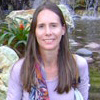
\includegraphics{../pictures/Maria.jpg}}
} &
\raisebox{1in}{\parbox{2.4in}{\textbf{Mar\'ia F. Arenas --- República Argentina} \textbf{(Author, Editor)} Independent consultant researcher on TICS applied to
Learning, Digital Communication, Institutional, Corporate. On line
facilitator tutorship. Professor on Semiotics, Social Communication,
Networking. \href{https://plus.google.com/u/0/stream/circles/p2e54657d0d6fc86d}{Mar\'ia
on Google+} \textbar{} \textbf{
}\href{http://arenastudies.wordpress.com/}{Mar\'ia's personal website}}}
\end{tabular}

\marktransitionempty

\begin{tabular}{lp{2.5in}}
\raisebox{.3in}{
\href{http://peeragogy.org/wp-content/uploads/2012/04/Regis.jpg}{

\includegraphics{../pictures/Regis.jpg}}
} &
\raisebox{1in}{\parbox{2.4in}{\textbf{R\'egis Barondeau --- Canada} \textbf{(Author)} I build bridges between
research, praxeology and technology and I become creative ``by finding a
likeness between things which were not thought alike before''
(Bronowski, 1958). I'm interested in complexity, culture, social media
especially wikis, education, open government and more.
Reach \href{https://twitter.com/regisbarondeau}{R\'egis on Twitter}
\textbar{} \href{http://www.regisbarondeau.com}{Regis' personal website}}}
\end{tabular}

\marktransitionempty

\begin{tabular}{lp{2.5in}}
\raisebox{.3in}{
\href{http://peeragogy.org/wp-content/uploads/2012/04/Doug.jpg}{

\includegraphics{../pictures/Doug.jpg}}
} &
\raisebox{1in}{\parbox{2.4in}{\textbf{Doug Breitbart --- USA, NJ (Author, Meeting Support)} I a
catalyst and provocateur who has worn the hats of attorney, consultant,
facilitator, coach, entrepreneur, father, husband, student, teacher.
\href{http://www.linkedin.com/profile/view?id=791427\&trk=tab\_pro}{Doug
on LinkedIn} \textbar{} \href{www.ontologique.com}{Doug's personal
website}}}
\end{tabular}

\newpage
\marktransitionempty

\begin{tabular}{lp{2.5in}}
\raisebox{.3in}{
\includegraphics{../pictures/Suz.jpg}}
&
\raisebox{1in}{\parbox{2.4in}{\textbf{Suz Burroughs - USA, CA} \textbf{(Author, Designer)} I enable the connections between the teacher and learner in all of us by designing robust, measurable learning environments where people share their knowledge and experience with each other. Learning Designer, Design Thinking facilitator, Visiting Professor of Innovation.
\href{http://susanburroughs.squarespace.com/}{Suz' personal website} }}\\
\end{tabular}

\marktransitionempty

\begin{tabular}{lp{2.5in}}
\raisebox{.3in}{
\href{http://peeragogy.org/wp-content/uploads/2012/04/Joe.jpg}{

\includegraphics{../pictures/Joe.jpg}}
} &
\raisebox{1in}{\parbox{2.4in}{\textbf{Joe Corneli --- U.K.} \textbf{(Author, Editor)} Joe Corneli does research on the anthropology of modern mathematics. He is a member
of the board of directors of the US-based nonprofit, PlanetMath.org,
and a research student at the Knowledge Media Institute of The Open
University, UK.  Reach \href{http://identi.ca/arided}{Joe on Identi.ca}
\textbar{} \href{http://metameso.org/\ensuremath{\sim}joe\%20}{Joe's
personal website}}}
\end{tabular}


\marktransitionempty

\begin{tabular}{lp{2.5in}}
\raisebox{.3in}{
\href{http://peeragogy.org/wp-content/uploads/2012/04/Jay.jpg}{

\includegraphics{../pictures/Jay.jpg}}
} &
\raisebox{1in}{\parbox{2.4in}{\textbf{Jay Cross --- USA, CA} \textbf{(Author)} Jay is the Johnny Appleseed of informal learning. The \href{http://internettimealliance.com/}{Internet Time Alliance}, which he chairs, helps corporations and governments use networks to accelerate performance.
\href{mailto:jaycross@internettime.com}{Jay by email} \textbar{}
\href{http://jaycross.com/}{Jay's personal website}}}
\end{tabular}

\newpage
\marktransitionempty

\begin{tabular}{lp{2.5in}}
\raisebox{.3in}{
\href{http://peeragogy.org/wp-content/uploads/2012/04/Charlie.jpg}{
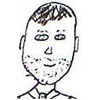
\includegraphics{../pictures/Charlie.jpg}}
} &
\raisebox{1in}{\parbox{2.4in}{\textbf{Charles Jeffrey Danoff --- USA, IL} \textbf{(Author)} Charles is the Owner of Mr.
Danoff's Teaching Laboratory, an Educational Publishing and Services
firm he established in 2009.  He started co-publishing
research on Paragogy, Peeragogy's inspiration, in late 2010.
\href{http://identi.ca/mrd}{Charles on Identi.ca} \textbar{}
\href{http://mr.danoff.org}{Charles' personal website}}}
\end{tabular}

\marktransitionempty

\begin{tabular}{lp{2.5in}}
\raisebox{.3in}{
\includegraphics{../pictures/James.jpg}}
&
\raisebox{1in}{\parbox{2.4in}{\textbf{James Folkestad - USA, CO (Author, Editor, Designer, Developer)} My approach to
education has shifted from an emphasis on my teaching, to a more central
focus on student learning, and finally to an activity-systems approach
as I have come to realize that the two (teacher and learner) are
inseparable parts of the learning ecosystem. Reach
\href{https://plus.google.com/u/0/114552232610071440407/about}{James on
Google+} \textbar{} \href{http://edgility.net}{James' personal
website} }}\\
\end{tabular}


\marktransitionempty

\begin{tabular}{lp{2.5in}}
\raisebox{.3in}{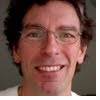
\includegraphics{../pictures/John.jpg}}
&
\raisebox{.8in}{\parbox{2.4in}{\textbf{John Graves - Australia (Editor)} 

Founder of SlideSpeech. Graduate of Singularity University. \medskip

Reach \href{http://twitter.com/slidespeech}{John on Twitter} \textbar{} \href{http://slidespeech.tumblr.com/}{John's personal website} }}\\
\end{tabular}

\marktransitionempty

\begin{tabular}{lp{2.5in}}
\raisebox{.3in}{
\href{http://peeragogy.org/wp-content/uploads/2012/04/Gigi.jpg}{
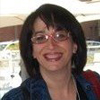
\includegraphics{../pictures/Gigi.jpg}}
} &
\raisebox{1in}{\parbox{2.4in}{\textbf{Gigi Johnson, EdD --- USA, CA (Author, Developer)} I mix formal learning
programs with programs to help learners begin to work, live, and create
everywhere. My own adventures include writing, singing, video, teaching,
and parenting 3 teens. \href{http://twitter.com/maremel}{Gigi on
Twitter} \textbar{} \href{http://maremel.com}{Gigi's personal
page}}}
\end{tabular}

\marktransitionempty

\begin{tabular}{lp{2.5in}}
\raisebox{.3in}{
\href{http://peeragogy.org/wp-content/uploads/2012/04/Anna.jpg}{
\includegraphics{../pictures/Anna.jpg}}
} &
\raisebox{1in}{\parbox{2.4in}{\textbf{Anna Keune --- Germany/Finland} \textbf{(Co-author, Designer)} I design technology for learning and I like it.  I'm affiliated with the Media Lab Helsinki, Aalto University School of Arts, Design and Architecture.
\href{https://twitter.com/\#!/akeune}{Anna on Twitter} \textbar{}
\href{http://www.annakeune.com}{Anna's personal website}}}
\end{tabular}

\marktransitionempty

\begin{tabular}{lp{2.5in}}
\raisebox{.3in}{
\href{http://peeragogy.org/wp-content/uploads/2012/04/kyle.jpg}{
\includegraphics{../pictures/Kyle.jpg}}
} &
\raisebox{1in}{\parbox{2.4in}{\textbf{Kyle Larson --- FL, USA (Editor)} 
Kyle Larson is an undergraduate thesis student at New College of Florida. His research interests include composition theory, rhetorical theory, computers and composition, and pedagogy.
\href{https://plus.google.com/110988036495982155492/posts}{Kyle on Google+}}}
\end{tabular}

\marktransitionempty

\begin{tabular}{lp{2.5in}}
\raisebox{.3in}{
\href{http://peeragogy.org/wp-content/uploads/2012/04/Roland.jpg}{
\includegraphics{../pictures/Roland.jpg}}
} &
\raisebox{1in}{\parbox{2.4in}{\textbf{Roland Legrand --- Belgium (Author)} I'm a financial journalist, heavily
involved in experimenting with social media and new forms for reporting
and community conversation.
\href{http://www.twitter.com/rolandlegrand}{Roland on Twitter}
\textbar{} \href{http://www.mixedrealities.com}{Roland's personal
website}}}
\end{tabular}

\marktransitionempty

\begin{tabular}{lp{2.5in}}
\raisebox{.3in}{
\href{http://peeragogy.org/wp-content/uploads/2012/04/Amanda.jpg}{
\includegraphics{../pictures/Amanda.jpg}}
} &
\raisebox{1in}{\parbox{2.4in}{\textbf{Amanda Lyons --- \textbf{USA}, NY} \textbf{Designer}\textbf{}I am a Visual
Practitioner, Organization Development Consultant \& Experiential
Educator. I love helping people communicate via visual tools that
generally include markers and paper. I think our education system could benefit from using visual communication tools as well as
text based methods. Reach
\href{https://twitter.com/\#!/amanda\_lyons}{Amanda on Twitter}
\textbar{} \href{http://www.visualsforchange.com/blog\%20\%20}{Amanda's personal website}}}
\end{tabular}

\marktransitionempty

\begin{tabular}{lp{2.5in}}
\raisebox{.3in}{
\href{http://peeragogy.org/wp-content/uploads/2012/04/Christopher.jpg}{
\includegraphics{../pictures/Christopher.jpg}}
} &
\raisebox{1in}{\parbox{2.4in}{\textbf{Christopher Neal --- USA, WA} \textbf{(Communications and Media)} I am driven by
technology and its ability to modify virtual communities and social
media, and a passion for Social:Learn, Social:iA, Situated
Cognition, Social Learning Theory, Connectivism, etc. 
\href{https://plus.google.com/u/0/106960445015668581969/posts}{Christopher
on Google+} \textbar{}
\href{http://beyondcredentials.com/index.php?option=com\_bc\_profile\_pages\&uname=berkeleyalum}{Christopher's
personal
website}}}
\end{tabular}


\marktransitionempty

\begin{tabular}{lp{2.5in}}
\raisebox{.3in}{
\vspace{-1em}
\href{http://peeragogy.org/wp-content/uploads/2012/04/Ted.jpg}{
\includegraphics{../pictures/Ted.jpg}}
\vspace{-2em}
} &
\raisebox{1in}{\parbox{2.4in}{\textbf{Ted Newcomb --- USA, AZ} \textbf{(Author, Project Management)} Happily retired grandpa, curating on digital culture,
sociology of the web; interested in collaboration and cooperation in
digital networks that result in positive change.
\href{http://about.me/tcnewcomb}{Ted on About.me} \textbar{}
\href{http://www.tcnewcomb.com}{Ted's personal website}}}
\end{tabular}

\marktransitionempty

\begin{tabular}{lp{2.5in}}
\raisebox{.3in}{
\vspace{-1em}
\href{http://peeragogy.org/wp-content/uploads/2012/04/Howard.jpg}{
\includegraphics{../pictures/Howard.jpg}}
\vspace{-1em}
} &
\raisebox{1in}{\parbox{2.4in}{\textbf{Howard Rheingold --- USA, CA} \textbf{(Author, Editor)} Inspired by
Charles Danoff and Joe Corneli's work on paragogy, I instigated the
Peeragogy project in order to provide a resource for self-organizing
self-learners. Learning is my passion. Reach
\href{https://twitter.com/\#!/hrheingold}{Howard on Twitter} \textbar{}
\href{http://www.rheingold.com}{Howard's personal
website}}}
\end{tabular}

\marktransitionempty

\begin{tabular}{lp{2.5in}}
\raisebox{.3in}{
\vspace{-1em}
\href{http://peeragogy.org/wp-content/uploads/2012/04/Paola.jpg}{
\includegraphics{../pictures/Paola.jpg}}
} &
\raisebox{1in}{\parbox{2.4in}{\textbf{Paola Ricaurte --- Mexico} \textbf{(Author)} My believe: education and
technology are essential tools for social change. My challenges:
activist, teacher, mother, immigrant. My philosophy: I am what I am
because of who we all are.
\href{https://twitter.com/paolaricaurte}{Paola on Twitter} \textbar{}
\href{http://blogs.eluniversal.com.mx/virtualis/}{Paola's personal
website}}}
\end{tabular}

\begin{tabular}{lp{2.5in}}
\raisebox{.3in}{
%\vspace{-1em}
\href{http://peeragogy.org/wp-content/uploads/2012/04/Paola.jpg}{
\includegraphics[width=1.4in]{../pictures/fabrizio.jpg}}
} &
\raisebox{1in}{\parbox{2.4in}{\textbf{Fabrizio Terzi --- Italy} \textbf{(Inventor, Designer, Translator)} 
I am involved in social and educational projects related to public access to knowledge and cultural diversity. I am an active member of FSF and the FTG -- working on Free Culture.
\href{http://identi.ca/siar}{Fabrizio on Identica} \textbar{}
\href{http://theftgacademy.org/}{Fabrizio's personal website}}}
\end{tabular}

\marktransitionempty

\begin{minipage}{3in}
\textbf{Geoff Walker --- U.K. (Author)} A Further and Higher Education Lecturer
and Tutor, social networker, e-learning advocate. \href{https://twitter.com/\#!/geoffreyawalker}{Geoff on
Twitter} \textbar{} \href{http://geoffreyawalker.blog.co.uk}{Geoff's
personal website}  
\begin{center}
\href{http://peeragogy.org/wp-content/uploads/2012/04/Geoff.jpg}{
\includegraphics{../pictures/Geoff.jpg}}
\end{center}
\end{minipage}

%
%\chapter[\textbf{License}]{License}
%
%\endnumbering
%\cleardoublepage
%\chapter[\textbf{Web pages referenced in this book}]{}
%\doendnotes{A}

\cleardoublepage
%\let\oldtwocolumn\twocolumn
%\renewcommand{\twocolumn}[1][]{#1}
\begingroup
\renewcommand{\cleardoublepage}{}
\renewcommand{\clearpage}{}
\chapter{Web Pages Cited in This Book}
\renewcommand{\indexname}{}
\vspace{-1in}
\onecolindex
\begingroup
%\let\oldurl\url
%\renewcommand*{\UrlFont}{\ttfamily\smaller\relax}
\smaller
\printindex
\endgroup
\endgroup
%\renewcommand{\twocolumn}[1][]{\oldtwocolumn}

\newpage
\chapter[\textbf{License/Waiver}]{License/Waiver}
These materials are made available under the terms of
\href{http://creativecommons.org/publicdomain/zero/1.0/}{Creative
Commons 0 copyright waiver} instead of a ``traditional'' copyleft
license. We the undersigned agree to the following, wherein ``this
work'' refers to ``The Peeragogy Handbook'' and all other content posted
on peeragogy.org or the original
collaboratory site, socialmediaclassroom.com/host/peeragogy.

\bigskip
\textbf{I hereby waive all copyright and related or neighboring rights
together with all associated claims and causes of action with respect to
this work to the extent possible under the law.}

\bigskip
Signed:

\begin{itemize}
\item
  Bryan Alexander
\item
  Paul Allison
\item
  Régis Barondeau
\item
  Doug Breitbart
\item
  George Brett
\item
  Suz Burroughs
\item
  Teryl Cartwright
\item
  Joseph Corneli
\item
  Jay Cross
\item
  Charles Jeffrey Danoff
\item
  Julian Elve
\item
  María Fernanda
\item
  James Folkestad
\item
  John Glass
\item
  Kathy Gill
\item
  John Graves
\item
  Gigi Johnson
\item
  Anna Keune
\item
  Kyle Larson
\item
  Roland Legrand
\item
  Amanda Lyons
\item
  Christopher Tillman Neal
\item
  Ted Newcomb
\item
  Stephanie Parker
\item
  Charlotte Pierce
\item
  David Preston
\item
  Howard Rheingold
\item
  Paola Ricaurte
\item
  Verena Roberts
\item
  Stephanie Schipper
\item
  Peter Taylor
\item
  Fabrizio Terzi
\item
  Geoff Walker
\end{itemize}
Note that this waiver does not apply to other works by the above
authors, including works linked to from
\href{http://peeragogy.org}{peeragogy.org}. It also does not apply to
embedded content drawn from other sites and included for the reader's
convenience.

Future contributors: Note also that we will require a similar
copyright waiver agreement from you.  That said, the waiver also means
that you are free to do essentially whatever you like with the content
in your own work!  Have fun!

\subsubsection{How we came to this decision}

These Creative Commons license options were proposed by various members
of the community:

\begin{itemize}
\item
  \emph{CC Zero} - public domain; no restrictions for downstream users
\item
  \emph{CC By-SA} - requires downstream users to include attribution and
  to license their work in the same way
\item
  \emph{CC By-SA-NC} - requires downstream users to include attribution,
  to license their work in the same way and disallows any commercial use
  of the content
\end{itemize}
After a brief discussion, no one was in favor of restricting downstream
users, so we decided to go with CC0. We agreed that we would get enough
``credit'' by having our names on
\href{http://peeragogy.org/}{peeragogy.org}. In connection with this
discussion, we agreed that we would work on ways to explicitly build
``reusability'' into the handbook content.

%
\pagestyle{empty} \thispagestyle{empty}
\clearpage\mbox{}\clearpage\mbox{}\clearpage\mbox{}\clearpage    %% blank pages

\end{document} %%%%%%%%%%%%%%%%%%%%%%%%%%%%%%%%%%%%%%%%%%%%%%%%%%%%%%%%%%%%%%%%%%%%%%%%%%%%%%%%%%%%%%%%%%%%%%%%%%%%

%% \chapter[\textbf{Use Cases}]{ Use Cases }
%% \section*{From peer production to peer learning}
%% \subsubsection{Main actor}

Julian, an enthusiastic convert to the power of peer-learning.

\subsubsection{Main success scenario}

\begin{enumerate}
\item
  Reflecting on the success
  of~\href{http://socialmediaclassroom.com/host/peeragogy/forum/patterns-and-use-cases\#comment-1749}{Strategy
  as Learning}, Julian notes that other housing associations might
  benefit from this process. He also notes that as most
  housing~association boards are made up of volunteers like himself,
  there is a very wide variation in background, knowledge and skills,
  and therefore not only a need for low cost~(free) learning
  opportunities, but a range of skills available to enable them.
\item
  Julian sets up a peer learning resource on the web, drawing on the
  experiences in
  implementing~\href{http://socialmediaclassroom.com/host/peeragogy/forum/patterns-and-use-cases\#comment-1749}{Strategy
  as Learning}, and promotes it through industry-specific web forums. He
  draws attention from an online journalist writing in the~housing field
  who writes a positive article, and as a result a growing number of
  collaborators come forward.
\item
  Over a period of a year or so, the core team of active users
  collaborate to create standards and exemplars in relation to different
  aspects of housing association governance that become a de facto
  standard in the sector.
\end{enumerate}

\subsubsection{Thoughts}

\begin{enumerate}
\item
  Obviously a very specific use case that could easily be generalised
\item
  Possible patterns to extract? Seeding Peer Communities, Emergent
  Standards, Emergent Assessment ???
\end{enumerate}

%% \section*{C’est la vie}
%% \subsubsection{Main Actors}

Pierre and Marie - recently married.

\subsubsection{Main Success Scenario}

\begin{enumerate}
\item
  They furnished off an apartment from a Sears \& Roebuck sale. Their
  coolerator was crammed with TV dinners and ginger ale. (She couldn't
  cook.)
\item
  But when Pierre found work, the little money coming in worked out
  well. They got a hi-fi phono, and boy, did they let it blast -- Seven
  hundred little EPs, all rock, rhythm and jazz.
\item
  When the sun went down, the rapid tempo of the music sort of fell (for
  various reasons).
\item
  They bought a souped up Mercedes -- a cherry red '53 -- and drove it
  down to New Orleans to celebrate their anniversary.
\item
  ``C'est la vie,'' say the old folks, ``It goes to show you never can
  tell!''
\end{enumerate}
(Après Chuck Berry.)

\subsubsection{Thoughts}

I tried to use the familiar song to suggest that pæragogy works in
personal relationships, too. Compare the above story with this quote
from Leopold von Sacher-Massoch\ldots{}:

\begin{quote}
``That woman, as nature has created her and as man is at present
educating her, is his enemy. She can only be his slave or his despot,
but \emph{never his companion}. This she can become only when she has
the same rights as he, and is his equal in education and work.''

\end{quote}
I don't know if Sacher-Massoch is particularly reliable as a feminist.
But it \emph{is} interesting to look at ``companionship'' (along with
membership in the same age cohort) as a criterion for a peer-like and
working relationship in the story. It's unclear as to whether Pierre \&
Marie have ``equal'' roles (he found work, but it's not in any way
implied that she was working\ldots{} so how did she spend her time?
Etc.).

%% \section*{Distributed Project Management}
%% \subsubsection{Main Actor}

Kim, a Ph. D. student in Geography.

\subsubsection{Main success scenario}

\begin{enumerate}
\item
  Kim has 5 different people on her supervision team: some in her field,
  others from geology. They all have somewhat different ideas about what
  she should be doing with her thesis work. None of them are co-located.
  This situation can be quite frustrating.
\item
  Kim decides to go spend a few weeks working in close proximity to the
  one member of the team who she has the most rapport with. This will
  also give her a chance to be in touch with other students in her
  field.
\item
  In the mean time, she establishes contact with yet another researcher
  whose work is quite closely related to hers. Although he does not have
  any formal responsibilities or ties to her project, they are already
  colleagues in an academic sense, and they have more congruent views on
  what her project is about. After she visits her favorite supervisor,
  she may plan to spend a month or so visiting this other researcher in
  his home country.
\end{enumerate}
\subsubsection{Note}

I think this sort of networking to create an informal supervision team
happens fairly frequently for postgrad students in the UK system.
Certainly there are other examples of distributed project management -
e.g.~W3C working groups come to mind.

%% \section*{Improved adaptivity}
%% \subsubsection{Main Actor}

Madeleine, a student who is trying to learn real analysis.

\subsubsection{Main success scenario}

\begin{enumerate}
\item
  Madeleine has been using a peer-learning website for mathematics for a
  while now. When she gets stuck, she asks for help in context, and her
  request is brought to the attention of the appropriate community
  member, who improves the pedagogic quality of the material. This help
  enables her to solve math problems very effectively.
\item
  Now, however, the system's software is being updated. Instead of being
  solely a ``Web 2.0'' system for communicating about the subject, the
  system can keep track of new concepts that Madeleine is using in the
  problems she solves and the questions she asks. It can suggest
  heuristics that have been used by other students solving similar
  problems. (It knows about these things through a combination of
  textual analysis and ``tagging'' of text by Madeleine and other users,
  e.g. Natalie, who sometimes gives comments on problems that Madeleine
  solves.)
\item
  As the system grows and improves (through efforts of students and
  mentors), learning mathematics becomes increasingly easy. The material
  has been gone over by 100s of students and learning pathways are
  optimized. Madeleine sometimes can get a quick tutoring gig helping
  out another younger student, and make some money, but mostly she's
  thinking about what other subjects she will need to add to her
  portfolio in order to become an architect\ldots{} by the time she's
  23!
\end{enumerate}

%% \section*{Improving the efficacy of research funding}
%% \subsubsection{Main actor}

Javier, who works for the European Commission.

\subsubsection{Main success scenario}

\begin{enumerate}
\item
  Javier is interested in research topics like ``data analytics'' and
  ``emerging topics in ICT'' -- things that will influence learning
  technology in the next 5 years. He is also concerned about how best to
  fund work on new learning and teaching environments.
\item
  He wonders what the barriers and incentives are in this niche. ~For
  example, why does research work frequently not have the broad-scale
  societal impact that the EC hopes it might?
\item
  Javier is invited to a pæragogy event, in which some unexpected
  experts on ``broad scale impact'' help him understand that intensive
  funding for research is often not going to have the desired effect,
  since, for various reasons, even well-funded research projects are
  frequently not well connected to actual practice.
\item
  He starts to build pæragogy into funding calls: smaller pots of money
  going to projects that connect with what people actually do, working
  with partners like the Wikimedia Foundation and the Free Software
  Foundation to multiply effort by involving volunteers. ~It's time for
  him to take a well-earned vacation.
\end{enumerate}

%% \section*{Journalist enters the Whispering Gallery}
%% \subsubsection{Main actor}

Jorge Luis is a journalist for a London business paper.

\subsubsection{Main success scenario}

\begin{enumerate}
\item
  Jorge Luis writes on a daily and even hourly basis about the eurozone
  crisis. He uses social dashboards and curating tools and produces lots
  of curated stories about the causes of the problems, the stupidity of
  the continental europeans and how it will all end soon in complete and
  utter disaster. His sources are other journalists, well-known
  economists and famous bloggers.
\item
  On his way to the newsroom he usually passes St Pauls cathedral, where
  Occupy London people protest. He thinks they rather look like losers,
  except for one very interesting young lady. She tells him where he can
  find the center of the universe: at the Whispering Gallery of the
  cathedral. He thinks she is nuts, but also very beautiful and
  interesting, so he walks the 259 steps from ground level to the
  Gallery. Once he gets there, he realizes that the girl was right. It
  IS the center of the universe. There are murmurs to be heard there -
  it seems they come from everywhere. He hears about guilds and the
  craftsmen who built the cathedral. He learns about how proud they were
  and how they formed communities of practice, educating the
  uninitiated, teaching each other to create.
\item
  He returns to ground level. The girl is gone, but yet he feels happy.
  He realizes he can do more then repackage the social media streams,
  that there is more than Twitter-the-new broadcast medium. He starts a
  new journey: finding a guild, a community of practice, but restyled in
  a 21st century fashion. It will be more open, more connected to others
  then the old guilds. He will still use a social dashboard and curaring
  tools, but also he uses wikis, and synchronous communication. And most
  importantly, he starts building, together with others. For instance,
  together with the people formerly known as his readers. They will
  co-create the analysis, the search for solutions and sense-making,
  rather than helplessly listening to ``experts'', passively consuming
  the knowledge and information. Instead, they'll start building their
  own destiny as a community, and the newsroom will be part of the
  platform.
\end{enumerate}

%% \section*{Living the OER dream}
%% \subsubsection{Main Actor}

Charlie, who does tutoring and educational consulting, and who has been
doing research on paragogy.

\subsubsection{Main success scenario}

\begin{enumerate}
\item
  Charlie usually tutors one-on-one but has been putting work into
  understanding and exploring peer learning and peer production, putting
  it into practice on P2PU and in courses and projects with Howard
  Rheingold.
\item
  X-Y-Z peer learning theory (paragogy?) helps him design learning
  activities that work well for groups of students
\item
  He deploys the new model on \href{http://paragogy.net}{paragogy.net}
  as an educational startup, and realizes the ``OER dream''!
\end{enumerate}

%% \section*{Making our own tools}
%% \subsubsection{Main Actor}

Howard runs \href{http://www.rheingold.com/university/}{Rheingold
University} and teaches courses at UCB and Stanford.

\begin{enumerate}
\item
  Howard created the peeragogy project, as a place to experiment and
  learn: ``I want to experiment as much as possible with peeragogy, with
  the group of contributors here, with the co-learners in Rheingold U,
  and with other groups in the future. I want to personally use the
  tools we're building. I know something about how to do it, and can
  make substantial contributions. But I also am learning a lot about how
  to do it from others, and expect that to continue.''
\item
  Although ``bringing a volunteer project to completion {[}\ldots{}{]}
  isn't a guaranteed slam-dunk'', Howard learns by doing: ``If I had it
  to do over again, I would have thought out the work flow and
  delineated it before we started talking about how to do the project.''
\item
  With both frequent, and other less frequent, but thoughtful,
  contributors, the project continues to develop, and will indeed
  complete somehow (even if no one knew quite what to expect in
  advance). Howard and other contributors have learned a lot in the
  process - and this will be useful both for the duration of the
  peeragogy project, and in future projects. As hoped!
\end{enumerate}

%% \section*{Peer Learning on the Technical Edge}
%% \subsubsection{Main Actor}

Jess,~ a hacker and engineer who develops new libraries and programs
quickly and on the bleeding edge of new technologies.

\subsubsection{Main success scenario}

\begin{enumerate}
\item
  Jess develops something new and totally cool and drops the source code
  in GitHub.~ These tools are developed rapidly and are a much lighter
  ``learning lift'' than learning say an entirely new programming
  language.
\item
  She creates documentation for her new library and puts it up on a web
  site for other developers to read.
\item
  She is trying to find a better way for other developers to learn how
  to use the new tools and libraries she creates and starts thinking
  about peer learning.
\item
  How can she use what tools and processes or methods that are already
  out there to engage other developers to learn from and with each other
  digitally? (Jess has no background in learning theory and is not in
  the educational field.)~ She finds the peeragogy handbook and a lot of
  this stuff starts to click.
\end{enumerate}

%% \section*{Prolegomena to Any Future Math Learning Environment}
%% \subsubsection{Main Actor}

A student, Madeleine, who is trying to learn multivariable calculus.

\subsubsection{Main Success Scenario}

\begin{enumerate}
\item
  Madeleine is enrolled in an advanced calculus course at university.
  She learns about PlanetMath from her instructor who recommends it as a
  place for extra practice with homework problems. Madeleine creates an
  account, fills in basic profile information, and starts solving
  problems that the system supplies based on the information she
  supplied in her profile.
\item
  The problems that the system supplies are automatically linked to
  reference resources in PlanetMath's encyclopaedia. This expository
  material gives Madeleine easy access to the relevant mathematical
  concepts, examples, and hints needed for solving the increasingly
  difficult practice problems. However, she eventually runs into a
  problem where neither the automatically supplied information, nor her
  current knowledge of the subject, is sufficient. She's completely
  stuck on a problem having to do with water flow in a pipe! Madeleine
  attaches a help request to the problem: ``I understand that I have to
  use the two variables \emph{x} and \emph{y} to solve for water flow,
  but I don't understand what the boundary limits of the equations would
  be: do I have to convert it to polar coordinates?"
\item
  This request is noticed by Natalie, a mathematics graduate student who
  regularly looks at the feed showing ``recent requests for help with
  advanced calculus.'' She sees that the reference resources linked to
  Madeleine's problem are probably not sufficient, and that Madeleine's
  idea about using polar coordinates would work. Natalie makes some
  changes to the encyclopaedia indicating that converting to converting
  to polar coordinates can be necessary in pipe flow problems, and
  sketches an example. Natalie then checks that this information links
  to Madeleine's problem correctly, and alerts Madeleine to the changes.
  With this new information, Madeleine is not only able to solve her
  problem, but can proceed with confidence: she had the right idea after
  all!
\end{enumerate}

%% \section*{Peeragogy helps solve complex problems}
%% \subsubsection{Main Actor}

Neo, who is a hacker by night, and an office worker by day (and who
reads Baudrillard in his spare time).

\subsubsection{Main Success Scenario}

\begin{enumerate}
\item
  Neo lives in New York City, and works as a programmer in an office
  near Wall Street. ~His day-job involves finding patterns in market
  data (see Kevin Slavin's
  \href{http://www.ted.com/talks/kevin\_slavin\_how\_algorithms\_shape\_our\_world.html}{TED
  talk}).
\item
  He has been walking
  past~\href{http://en.wikipedia.org/wiki/Zuccotti\_Park}{Zucotti
  Park}~on his way home and more or less he finds this protest stuff
  annoying (he has other stuff on his mind). ~But one of these evenings,
  one of the protestors catches his attention (she's dressed rather
  strikingly\ldots{}). ~They talk a bit, and he comes away thinking
  about what she said:
  ``\href{http://www.nycga.net/files/2011/11/DeclarationFlowchart\_v2\_large.jpg}{All
  our grievances are interconnected.}''~ What if all the solutions are
  interconnected too?
\item
  Night time: Neo becomes increasingly obsessed with this idea. ~He's
  pulling down lots of web pages from OWS activists, from companies,
  from government websites -- again, looking for patterns. ~What would
  it take for OWS folks to solve the problems they worry so much about?
\item
  He eventually stumbles across the idea of~pæragogy~and it~works like
  the ``red pill'': it's possible to solve the problems but only by
  working together. ~It would be hard to engineer a social media
  platform that will actually help with this (OWS folks mostly use
  Tumblr and aren't necessarily all that technologically minded). ~But
  he starts working on
  a~\href{http://campus.ftacademy.org/wiki/index.php/Free\_Technology\_Guild}{tool}~that's
  geared towards learning and sharing skills, while working on real
  projects. ~At first, it's just hackers who are using the tool, but
  over time they adapt it for popular use. ~Then things start to get
  interesting\ldots{}
\end{enumerate}

%% \section*{Starting a Company}
%% \subsubsection{Introduction}

I think that Peeragogy has flavors -- learning for learning sake for
personal ends in a progression toward learning about the world to take
action as a group. The latter gets heavily into Action Research
(Stringer, 2007), which I love and work heavily in. It is research in
cycles, or loops with feedback to try something, measure it, see how it
worked with the real world, then plan the next question and set of
actions. In each cycle, the group is Learning. I look with that lens at
company start-ups as a perpectual action research cycle. I heard Eric
Reis at SXSW talk about the Lean Startup in this mode, including this
direction in how he even wrote the book. Hypothesis, experiment,
feedback, learn, pivot, next hypothesis\ldots{} Is the group in this
peeragogy learning set knowledge or creating new knowledge? Or through
new knowledge making a change in the world? A great spectrum of
alternatives! Here, my scenario about a company I was on the board on
early on:

\subsubsection{Main actors}

\begin{itemize}
\item
  Cycle 1: Nick, an MBA student, plus a Computer Science PhD, John, at a
  major university. John had created a unique technology for identifying
  video clips and had no idea what to do with it. Nick was an
  ex-engineer learning about how to launch new businesses.
\end{itemize}
\begin{itemize}
\item
  Cycle 2: Additional ``learners'' and co-teachers as board members,
  each adding new learning elements and expertise.
\end{itemize}
\begin{itemize}
\item
  Cycle 3+: New learners as investors and clients.
\end{itemize}
\subsubsection{Main success scenario}

\begin{enumerate}
\item
  Nick and John used a new business plan competition as the catalyst and
  structure to experiment with what ideas might be possible to grow this
  idea. They named it Findable (not the real name; the company did
  launch with some interesting success, but we'll come to that later).
  They brought three other MBAs into the initial group, and within the
  confines of a business plan structure, researched the stereotypical
  elements of a business plan -- addressable market, competition,
  expense and revenue projections, etc. They knew nothing of the area,
  and each person did independent research work to provide some primary
  (interview-based) and secondary (existing text) information about
  their hypothesis of what the technology could do for what audience in
  what environment. They worked hard up until the competition deadline,
  and won the business plan competition, gaining \$15,000 in the process
  plus the attention of some VCs on the judging panel. Each person had
  learned a lot about the technology, the creative process of writing
  the business plan, the rituals involved of asking for money, and the
  flaws in their own plan that they found on its creation. They used
  fairly traditional technology tools: email, shared Word and Excel
  files, telephone, search, and a shared file system to store everything
  that they worked on.
\item
  Nick and Fred wanted to move forward with this project. Their next
  hypothesis was that they could launch this in a specific market. They
  first came to the idea, from the learning from the business plan and
  lots of feedback from the VCs, that they could start with the
  advertising market, as they could now identify and ``tag'' any ad that
  they could find on cable or the internet. They got seed capital from
  three interested parties, who become part of their Action Research
  learning team. They realized to launch that they needed more voices on
  their learning team, so they added their first 3 employees to design
  and sell the product. They also added an advisory board, including
  yours truly, assuming they would be working in the advertising market.
  Technologies? Traditional, though they now included all sorts of tech
  development resources. New information into the mix? They had not put
  together great resources to optimize their time learning, and spent a
  lot of energy keeping up with things, information, and opportunities.
  Learning? Some initial users loved their product, but the market size
  was smaller than they thought\ldots{}plus was very entrenched. The
  companies did not see a real pain point that was being solved.
\item
  Cycle 3 -- what the heck do Nick and Fred do with this? This became
  the true learning phase. Different companies and advisors saw
  different needs for their intriguing product set. They spent 4 years
  (!!!) getting pulled this way and that, using the VC money and needing
  more. (This is VERY much the learning path I see in many small tech
  companies.) Technologies? Same stuff. Learning team? Ebbed and flowed
  with new opportunities and people's patience. My expertise was in the
  ``old'' model, so peaceably left the team (but got options!).
\item
  Cycle 4+ -- a major public company ``found'' them through their
  learning cycles, and found that they solved a pain point. They
  invested a sizeable sum into a chunk of the company, and launched
  their product into that solution. This opened a whole other set of
  learning doors.
\item
  Final cycle -- Happily, I cashed out my options. Two major media
  technology companies ended up buying two areas of key technologies in
  2011, much to my own pocketbook's happiness. Nick and Fred had moved
  on earlier, turning the company learning over to specialized managers.
  I need to see what Nick is up to next\ldots{}.
\end{enumerate}
\subsubsection{Thoughts}

\begin{enumerate}
\item
  Many great patterns were tucked into many cycles of this use case,
  often unspoken assumptions in a new business start-up, including
  environment scanning, codifying specialist knowledge, themes,
  modeling, etc. Consensus building -- an interesting element.
\item
  For me, the additional elements are (a) the scaffolding of the
  ``norms'' of cycles (e.g., business plan creation, a competition, a
  launch of a product) help provide ``norming'' frameworks that can help
  groups achieve as well as limit their looking at the structural norms
  as anything but ``required'' and (b) the lens of Action Research
  Cycles from my own POV. Are we setting a hard limit of providing a
  hypothesis in our co-creation, so we know when we are ``done'' and
  what we have to study? Then once that chunk is done (and CELEBRATED)
  that another hypothesis can be investigated, explored, proven, and
  co-created? I believe that having pre-structured points of learning
  achievement, reflection, and celebration can really help in moving
  forward.
\item
  My own brain is rethinking these issues around content creation after
  hearing Eric Reis speak on how he tested his content creation for his
  \emph{New York Times} best-selling book.
\item
  How are we testing this Handbook, other than living through it? :)
\end{enumerate}

%% \section*{Steal This Book}
%% "Obviously such a project as Steal This Book could not have been carried
out alone. Izak Haber shared the vision from the beginning. He did
months of valuable research and contributed many of the survival
techniques. Carole Ramer and Gus Reichbach of the New York Law Commune
guided the book through its many stages. Anna Kaufman Moon did almost
all the photographs. The cartoonists who have made contributions include
Ski Williamson and Gilbert Sheldon. Tom Forcade, of the UPS, patiently
did the editing. Bert Cohen of Concert Hall did the book's graphic
design. Amber and John Wilcox set the type. Anita Hoffman and Lynn
Borman helped me rewrite a number of sections. There are others who
participated in the testing of many of the techniques demonstrated in
the following pages and for obvious reasons have to remain anonymous.
There were perhaps over 50 brothers and sisters who played particularly
vital roles in the grand conspiracy. Some of the many others are listed
on the following page. We hope to keep the information up to date. If
you have comments, law suits, suggestions or death threats, please send
them to: Dear Abbie P.0. Box 213, Cooper Station, New York, NY 10003.
Many of the tips might not work in your area, some might be obsolete by
the time you get to try them out, and many addresses and phone numbers
might be changed.~\emph{If the reader becomes a participating researcher
then we will have achieved our purpose.}"~-- Abbie Hoffman (emphasis
added)

%% \section*{Strategy as learning}
%% \textbf{Main actors}

The non-executive (Jim, Pamela, Julian) and executive (Clare, Malcolm,
Colin \& Jenny) directors of a housing association (a not-for-profit
organisation building and letting ``social'' housing for families in
housing need) \textbf{Main success scenario}

\begin{enumerate}
\item
  The board of the housing association need to set a strategy that takes
  account of significant changes in legislation, the UK {[}welfare{]}
  benefits system and the availability of long term construction loans.
\item
  Julian, eager to make use of his new-found peeragogical insights
  suggests an approach where individuals research specific factors and
  the team work together to draw out themes and strategic options. As a
  start he proposes that each board member researches an area of
  specific knowledge or interest.
\item
  Jim, the Chairman, identifies questions he wants to ask the Chairs of
  other Housing Associations. Pamela (a lawyer) agrees to do an analysis
  of the relevant legislation. Clare, the CEO, plans out a series of
  meetings with the local councils in the boroughs of interest to
  understand their reactions to the changes from central government.
  Jenny, the operations director, starts modelling the impact on
  occupancy from new benefits rules. Colin, the development director,
  re-purposes existing work on options for development sites to reflect
  different housing mixes on each site. Malcolm, the finance director,
  prepares a briefing on the new treasury landscape and the changing
  positions of major lenders.
\item
  Each member of the board documents their research in a private wiki.
  Julian facilitates some synchronous and asynchronous discussion to
  draw out themes in each area and map across the areas of interest.
  Malcolm, the FD, adapts his financial models to take differet options
  as parameters.
\item
  Clare refines the themes into a set of strategic options for the
  association, with associated financial modelling provided by Malcolm.
\item
  Individual board members explore the options asynchronously before
  convening for an all-day meeting to confirm the strategy.
\end{enumerate}
\textbf{Thoughts}

\begin{enumerate}
\item
  This may be a little close to the ``peer production'' end of
  peeragogy, but on the other hand, where (if anywhere) do we draw the
  line?
\item
  This probably needs to be made a little more abstract to be a useful
  use case, and in doing so I suspect will start to overlap with
  \href{http://socialmediaclassroom.com/host/peeragogy/forum/patterns-and-use-cases\#comment-1509}{Pæragogy
  helps solve complex problems}
\item
  It looks to me as if there may be some candidate patterns buried in
  this use case, e.g.~Environment Scanning, Codifying Specialist
  Knowledge, Extracting Themes, Modelling Outcomes, Consensus Building
\end{enumerate}

%% \section*{We are the 1 percent}
%% \subsubsection{Main Actor}

Trinity, the daughter of a Texas oil magnate.

\subsubsection{Soundtrack}

\href{http://www.youtube.com/watch?v=NWsX9ggfL2Q}{You Make Me Like
Charity} by The Knife

\subsubsection{Main success scenario}

\begin{enumerate}
\item
  Trinity has spent the last year traveling around the world to join in
  various \#Occupy protests. Her aim is to get people in the movement
  thinking about how they can empower themselves.
\item
  It's tricky though, because as much as she knows she has an impact on
  individuals, she still sees a lot of problems in the world, which,
  given her manic-depressive tendencies, she tends to find very
  disturbing.
\item
  She reaches out to other folks who are privileged in one way or
  another -- and a bunch of ``normal folks'' -- trying not only to bring
  about political change, but trying to establish a degree of personal
  friendship and camaraderie, and a feeling of ``belonging in the
  world''. For her, this is a constant struggle. She finds that working
  with other people on concrete tasks keeps her from spiraling into a
  state of gloom. In the mean time, she's also building a tremendous
  amount of knowledge about the way social movements and political
  processes work.
\end{enumerate}
\subsubsection{Footnote}

``The Knife is now recording a new album to be released in 2012. Lately
we have read a lot about the ongoing discrimination of Romani people in
Europe which is totally unacceptable. The forced evictions must stop and
adequate alternative housing must be arranged. Now!'' --
\href{http://theknife.net/take-action-for-the-housing-rights-of-roma-in-rome}{The
Knife}

%% \section*{Young aspiring blogger wants to avoid starvation}
%% \subsubsection{Main actor: Simone}

Simone is a young media department graduate, who followed the adventures
of the journalist Jorge Luis. Jorge Luis was transforming the newspaper
operation into a kind of collective learning project, turning the
newsroom into a platform for discussion and learning, and inciting the
developers to provide an API for external coders. Simone wrote a paper
about all this in her last year at the media department.\textbf{~}She
also runs a blog about tools which empower people to participate in
politics (local, nation-wide and international).

\subsubsection{Main success scenario}

\begin{enumerate}
\item
  Simone loves her blog. She believes verticals and specialization are
  the future in blogging. However, she needs money to live, and to pay
  back the debts she made to finance her studies. Her media department
  was moderately interesting, but nobody ever thought of organizing a
  course ``entrepreneurial blogging/journalism''.
\item
  Posting every day about collaborative online tools such as wikis,
  forums, blogs, mindmaps, synchronous sessions, social bookmarks,
  visualization tools, Simone decides to reach out and look online for
  others who are experiencing the same challenges.
\item
  As she encounters various other people, they start curating stuff
  about blogging business models and best practices. They find lots of
  useful stuff for free at Robin Good's website, and they manage to get
  access to online resources at a strange group which seems to
  specialize in ``mind amplifying tools'' and ``literacies of
  cooperation''. They also discover that ``entrepreneurial journalism''
  is taught at various colleges, and invariably the professors and most
  of the students there indulge in blogging and publishing about their
  insights and experiments. All that material is being discussed on the
  collaborative platform Simone built.
\item
  Simone uses the discussions to blog about her experience. After all,
  issues about financing media who empower people in order to broaden
  and deepen the democracy is something which is rather on topic for her
  own blogging practice. Also, because of her reaching out, her contacts
  increased considerably. She works together with someone to share a
  virtual co-working space, and people start noticing her. Some ask her
  for customized expert advice about collaborative tools and
  collaboration methodologies. The city council expresses some vague
  interest and considers hiring her as a consultant.
\item
  Even though she gets several gigs, Simone realizes it's not easy to
  earn a living as a blogger. But it seems to open other doors\ldots{}
  however, she continues her investigation about business models for
  collaborative media. As yet we don't know whether Simone's blog will
  be profitable in itself, but we do see a network around her projects,
  exchanging insights but also valuable business information and opening
  more doors.
\end{enumerate}

\subsubsection{Thoughts}

I had the opportunity to give some seminars at media departments here in
Belgium. In my experience, the students were not familiar with curation
practices or infotention strategies. They also lack courses in
entrepreneurial journalism. In other words, they're still educated for
the big media companies, but they're not prepared to start the next
TechCrunch or Huffington Post. Often the students asked me, after the
seminar, ``how can we learn all this? they won't teach us these things
here''. I think there is a need for P2P learning about not only
curation, infotention, social dashboards, communities and governance of
common pool recourses, but also about publishing strategies, social
media workflows and business models.

